\chapter{\textcolor{azulescom}{Implementación}}

\section{Arquitectura del sistema}
La arquitectura final de implementación no difiere en gran medida de la arquitectura
discutida en el capítulo de diseño, sin embargo, se realizaron ajustes en función de
algunos retos encontrados durante la implementación. La arquitectura final del sistema
se muestra en la figura \ref{fig:arquitectura-final}.

\begin{figure}[H]
    \centering
    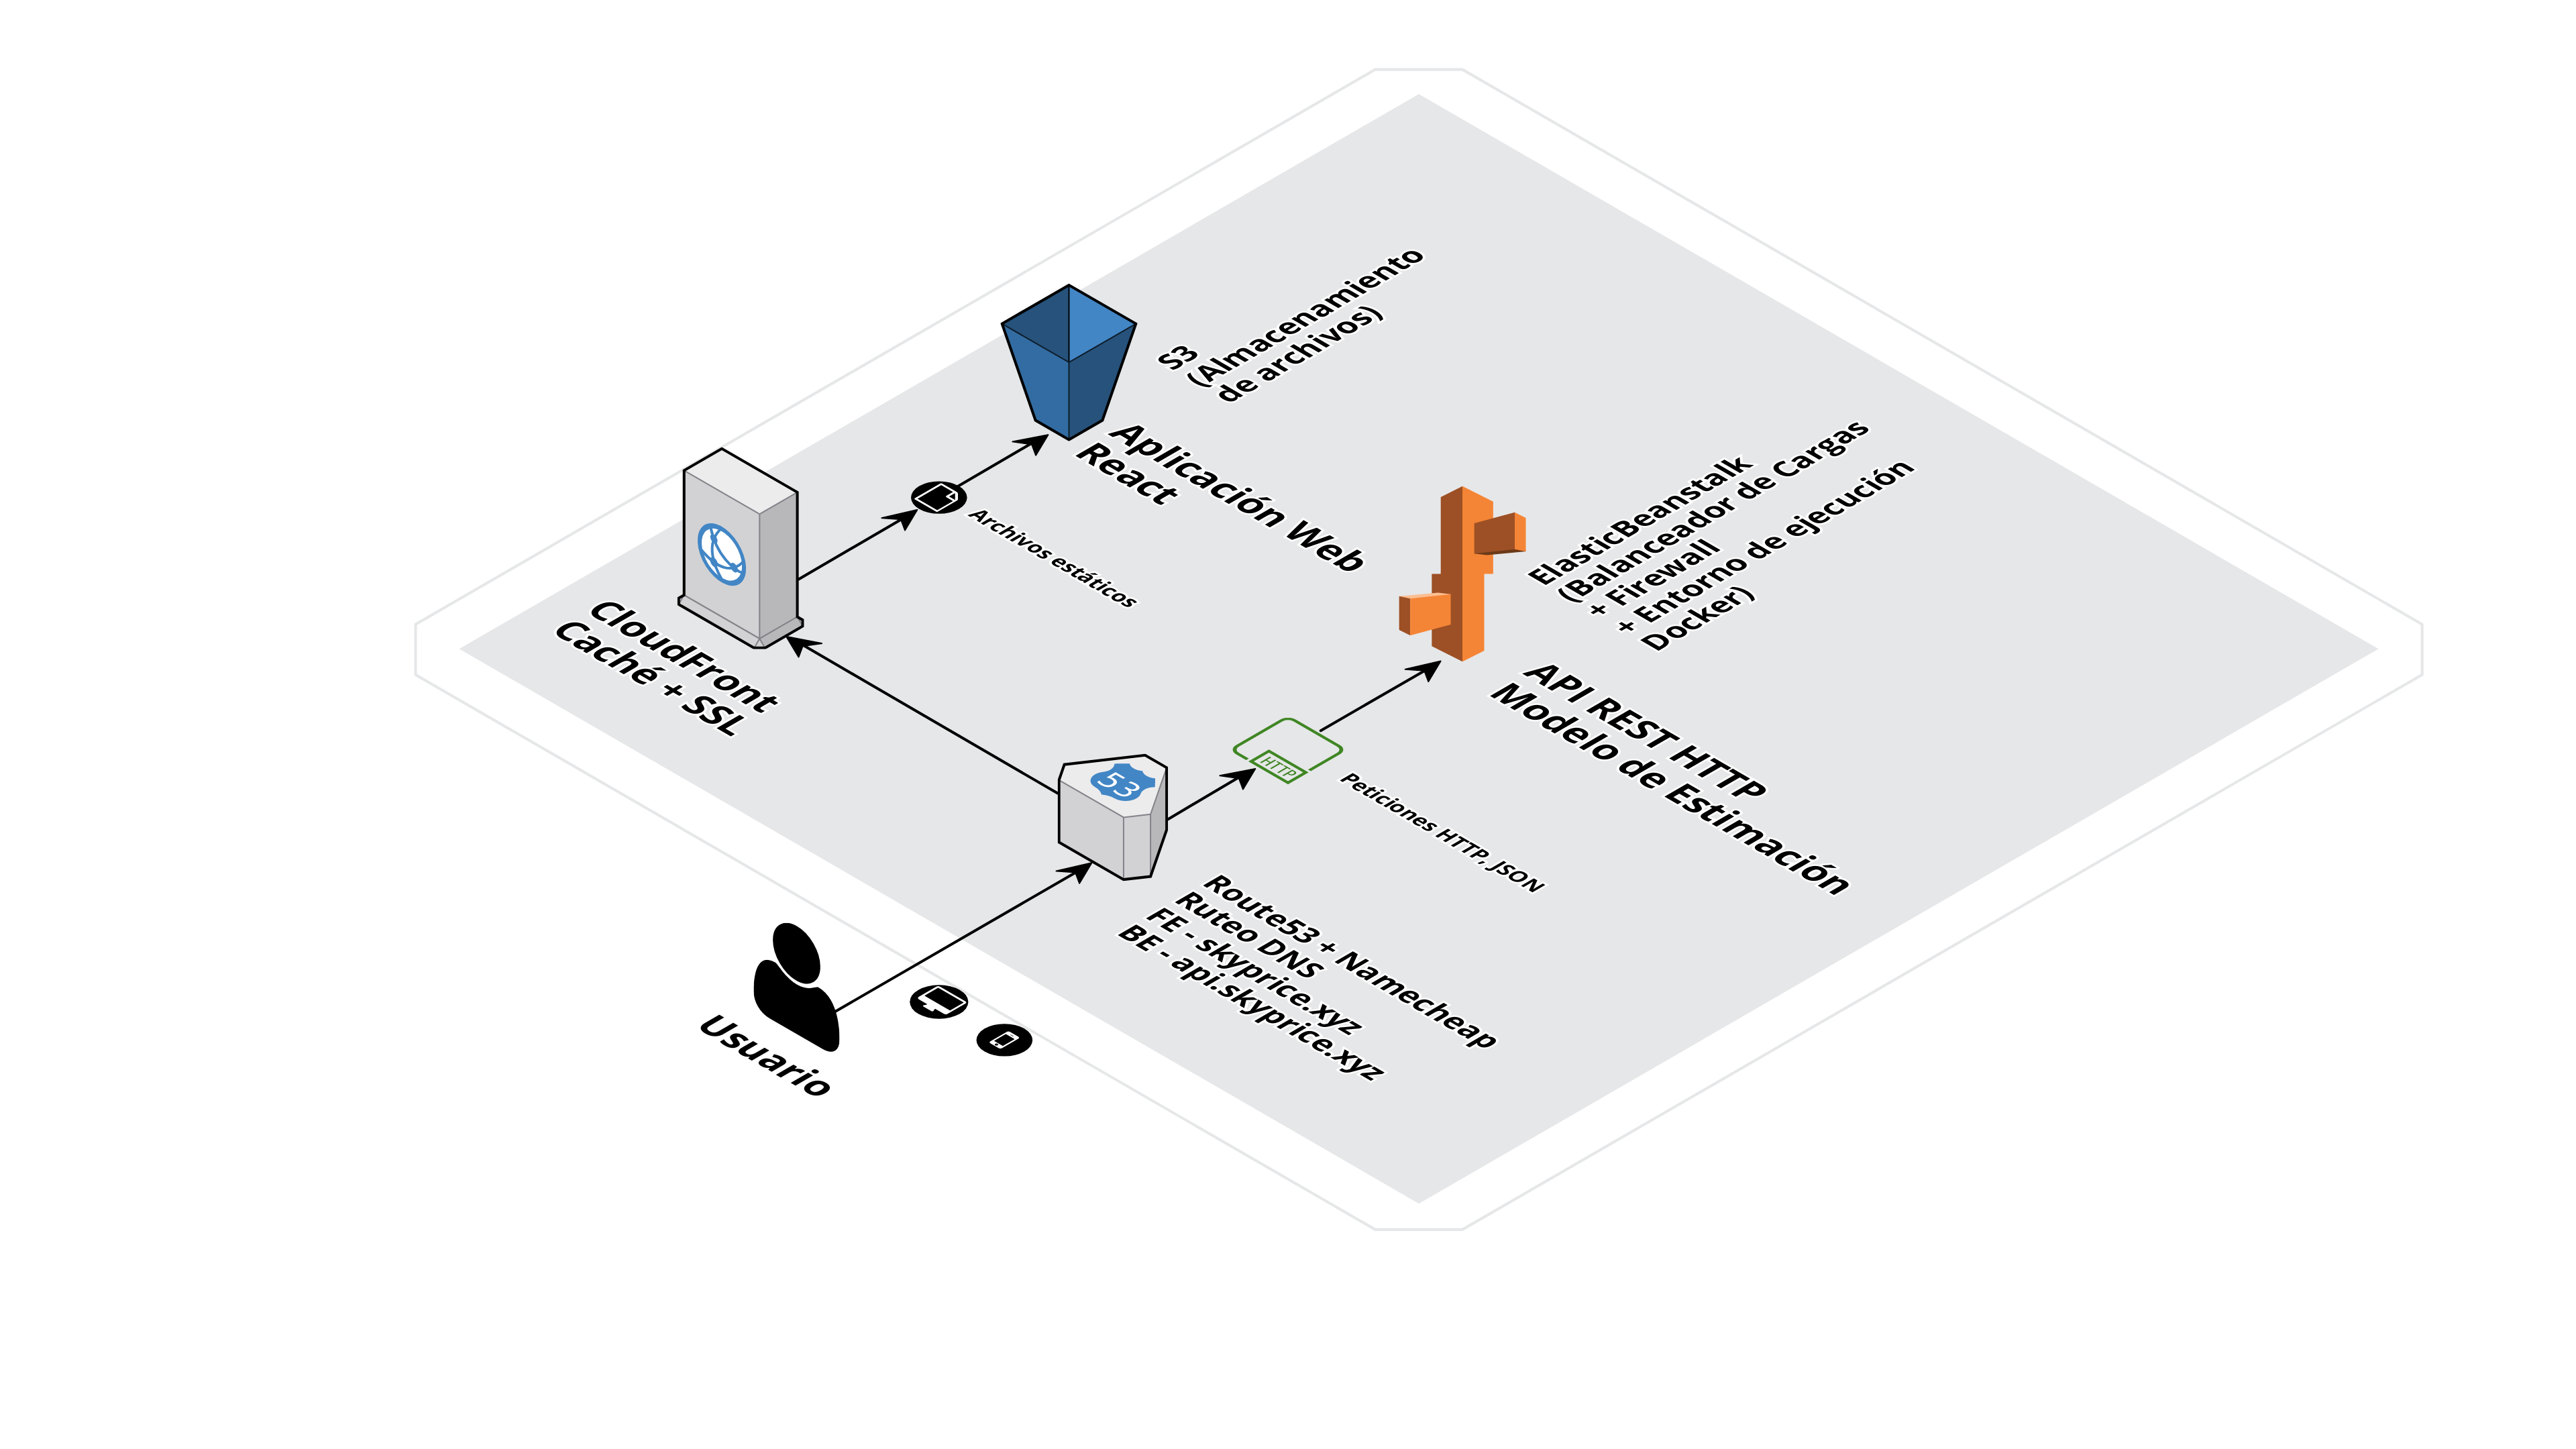
\includegraphics[width=1.0\textwidth]{imagenes/05-implementacion/arquitectura/arquitectura-final.png}
    \caption{Arquitectura final del sistema.}
    \label{fig:arquitectura-final}
\end{figure}

El único aspecto a destacar es la integración de Namecheap como proveedor de dominios
ya que Route53 de AWS no permite la compra de dominios con terminación \texttt{.xyz},
por lo que se optó por utilizar Namecheap para la compra del dominio \texttt{skyprice.xyz}.

\section{Desarrollo de los modelos}

En esta sección se abordarán todos los pasos empleados para concluir con el
desarrollo de los modelos de aprendizaje automático, empleando los datos descritos
previamente y afinando los hiperparámetros de los modelos.

\subsection{Conjunto de datos}
En la figura \ref{fig:conjunto-datos-finder} se muestra un vistazo de las características
del archivo CSV que se utilizó para el entrenamiento de los modelos. Este archivo
contiene la información sobre los departamentos en la Ciudad de México que será
utilizada para predecir el precio de las propiedades.

\begin{figure}[H]
    \centering
    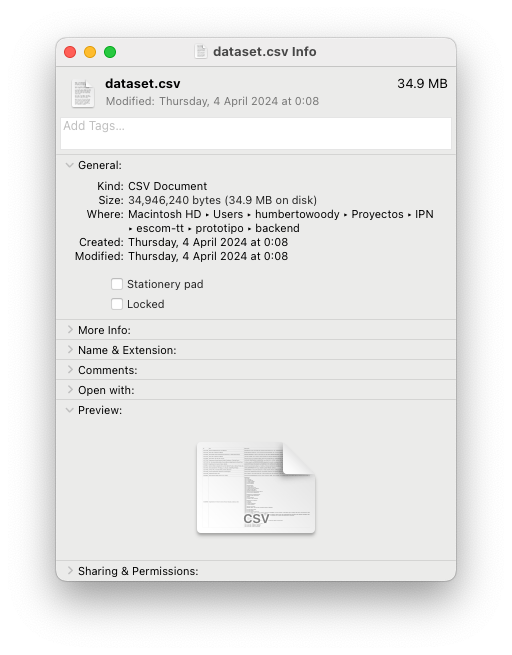
\includegraphics[width=0.5\textwidth]{imagenes/05-implementacion/desarrollo-modelos/conjunto-datos-finder.png}
    \caption{Vistazo al conjunto de datos utilizado para el entrenamiento de los modelos.}
    \label{fig:conjunto-datos-finder}
\end{figure}

\subsection{Preprocesamiento de los datos}
El preprocesamiento de los datos incluyó la limpieza de los mismos para eliminar
valores atípicos, ajustar los valores faltantes y normalizar las características.
Posteriormente, se comienza con la separación de los conjuntos de datos
de entrenamiento (75\% de los datos) y de prueba (25\% de los datos) y se crean
los escaladores para normalizar las características, utilizando un \texttt{StandardScaler}
para las características numéricas y un \texttt{OneHotEncoder} para las características categóricas.

En el listado \ref{lst:preprocesamiento} se muestra el código relevante para realizar
el preprocesamiento de los datos usando Python, con las librerías Pandas y Scikit-learn.

\begin{lstlisting}[language=python, caption={Preprocesamiento de los datos}, label={lst:preprocesamiento}]
# Dividir el dataset en conjuntos de entrenamiento y prueba
X = df[['Municipality','Size_Terrain', 'Size_Construction', 'Rooms', 'Bathrooms', 'Parking', 'Age', 'Lat', 'Lng']]
y = df['Price']
X_train, X_test, y_train, y_test = train_test_split(X, y, test_size=TEST_SIZE, random_state=RANDOM_STATE)
print(f'Dimensiones de los conjuntos de entrenamiento y prueba: {X_train.shape}, {X_test.shape}')

# Crear un preprocesador para las columnas numéricas
numeric_transformer = Pipeline(steps=[
    ('scaler', StandardScaler())
])

# Obtener las columnas numéricas
numeric_features=columnas_numericas[1:]

# Crear un preprocesador para las columnas categóricas
preprocessor = ColumnTransformer(
    transformers=[
        ('cat', OneHotEncoder(categories=[municipalities]), ['Municipality']),
        ('num', numeric_transformer,numeric_features),
    ])
\end{lstlisting}

\subsection{Entrenamiento de los modelos}
Cada algoritmo de aprendizaje automático se entrenó utilizando el conjunto de
datos de entrenamiento y se evaluó utilizando el conjunto de datos de prueba.
De esta manera, se pudo determinar la precisión de cada modelo y seleccionar
los hiperparámetros adecuados para cada uno.

Dado que las combinaciones de hiperparámetros son numerosas, se utilizó la
técnica de búsqueda en cuadrícula (\texttt{GridSearchCV}) para encontrar la
combinación óptima de hiperparámetros para cada modelo, el cual permite especificar
una cuadrícula de hiperparámetros y evaluar todas las combinaciones posibles \cite{sklearn_gridsearchcv}.

El tiempo de entrenamiento promedio para los tres modelos fue de aproximadamente
una hora con treinta minutos, esto debido a las permutaciones de hiperparámetros
resultantes de la búsqueda en cuadrícula, con el objetivo de realizar distintas
pruebas, se decidió por proveer de un modo reducido de hiperparámetros para
disminuir el tiempo de entrenamiento y poder realizar pruebas más rápidas, es
por esto que en varios fragmentos de código se puede observar la variable
\texttt{FAST\_TEST} que se encarga de seleccionar el modo reducido de hiperparámetros.

\subsubsection{Redes neuronales}
Las redes neuronales se implementaron usando TensorFlow y Keras, y se experimentó
con diferentes configuraciones de capas, neuronas y funciones de activación para
mejorar la precisión del modelo. A continuacón se muestran los hiperparámetros
utilizados en la búsqueda en cuadrícula para las redes neuronales.

\begin{itemize}
    \item Capas y neuronas por capa: [(10, 10), (10, 10, 10), (30, 30)]
    \item Dropout: [0.5, 0.7]
    \item Tamaño del conjunto de entrenamiento: [50, 100]
    \item Épocas: [50, 100, 200, 500]
    \item Tasa de aprendizaje: [0.1, 0.01, 0.001]
    \item Funciones de activación: ['relu', 'tanh', 'sigmoid']
\end{itemize}

Los parámetros cuyos valores no cambiaron son los siguientes:

\begin{itemize}
    \item Optimizador: Adam
    \item Función de pérdida: Mean Squared Error
\end{itemize}

Una vez finalizado el entrenamiento y selección del mejor modelo, se procedió
a exportar el modelo a un archivo \texttt{.h5} para su posterior importación en el
servicio web.

El código que se muestra en el listado \ref{lst:entrenamiento-redes-neuronales}
corresponde al entrenamiento de las redes neuronales, donde se utilizó la técnica
de búsqueda en cuadrícula para encontrar los mejores hiperparámetros.

\begin{lstlisting}[language=python, caption={Entrenamiento de redes neuronales}, label={lst:entrenamiento-redes-neuronales}]
# Preprocesar los datos para la red neuronal
X_train_preprocessed = preprocessor.fit_transform(X_train)

# Función para obtener el modelo de red neuronal
def get_reg(meta, hidden_layer_sizes, dropout):
    n_features_in_ = meta["n_features_in_"]
    model = keras.models.Sequential()
    model.add(keras.layers.Input(shape=(n_features_in_,)))
    for hidden_layer_size in hidden_layer_sizes:
        model.add(keras.layers.Dense(hidden_layer_size, activation="relu"))
        model.add(keras.layers.Dropout(dropout))
    model.add(keras.layers.Dense(1))
    return model

# Crear el modelo de red neuronal
reg = KerasRegressor(
    model=get_reg,
    loss=keras.losses.MeanSquaredError,
    optimizer=keras.optimizers.Adam,
    metrics=[keras.metrics.R2Score],
    hidden_layer_sizes=(100,),
    dropout=0.5,
)

# Parámetros a buscar
param_grid_nn_fast = {
    "hidden_layer_sizes": [(10, 10)],
    "dropout": [0.5],
    "batch_size": [50],
    "epochs": [50],
    "optimizer": [keras.optimizers.Adam],
    "optimizer__learning_rate": [0.1],
    "loss": [keras.losses.MeanSquaredError],
    "metrics": [keras.metrics.R2Score],
}
param_grid_nn_slow = {
    "hidden_layer_sizes": [(10, 10), (10, 10, 10), (30, 30)],
    "dropout": [0.5, 0.7],
    "batch_size": [50, 100],
    "epochs": [50, 100, 200, 500],
    "optimizer": [keras.optimizers.Adam],
    "optimizer__learning_rate": [0.1, 0.01, 0.001],
    "loss": [keras.losses.MeanSquaredError],
    "metrics": [keras.metrics.R2Score],
}
param_grid_nn = FAST_TEST and param_grid_nn_fast or param_grid_nn_slow

# Crear el objeto GridSearchCV
grid_search_nn = GridSearchCV(
    estimator=reg,
    param_grid=param_grid_nn,
    refit=False,
    cv=5,
    verbose=2,
    n_jobs=-1,
)

# Debido a que el preprocesamiento ya está hecho, podemos usar X_train_preprocessed directamente aquí
grid_search_nn.fit(X_train_preprocessed, y_train)

# Obtener los mejores parámetros
mejores_parametros = grid_search_nn.best_params_
\end{lstlisting}

\subsubsection{Random Forest}
El modelo de Random Forest se entrenó de igual manera que las redes neuronales,
utilizando la técnica de búsqueda en cuadrícula para encontrar los mejores hiperparámetros
como lo son el número de estimadores, la profundidad máxima y el mínimo de muestras
para bifurcar un nodo. A continuación se muestran los hiperparámetros utilizados
en la búsqueda en cuadrícula para el modelo de Random Forest:

\begin{itemize}
    \item Número de estimadores: [100, 500, 1000]
    \item Profundidad máxima: [None, 10, 20, 30]
    \item Mínimo de muestras para dividir: [2, 5, 10]
\end{itemize}

Una vez finalizado el entrenamiento y selección del mejor modelo, se procedió
a exportar el modelo a un archivo \texttt{.joblib} para su posterior importación en el
servicio web.

En el listado \ref{lst:entrenamiento-random-forest} se muestra el código relevante
para entrenar el modelo de Random Forest, utilizando la técnica de búsqueda en cuadrícula.

\begin{lstlisting}[language=python, caption={Entrenamiento de Random Forest}, label={lst:entrenamiento-random-forest}]
# Crear el pipeline
rf_pipeline = Pipeline(steps=[('preprocessor', preprocessor),
                              ('regressor', RandomForestRegressor(random_state=42, oob_score=True, n_jobs=-1))])

# Parámetros a buscar
param_grid_rf_fast = {
    'regressor__n_estimators': [100],
    'regressor__max_depth': [None],
    'regressor__min_samples_split': [2],
}
param_grid_rf_slow = {
    'regressor__n_estimators': [100, 500, 1000],
    'regressor__max_depth': [None, 10, 20, 30],
    'regressor__min_samples_split': [2, 5, 10]
}
param_grid_rf = FAST_TEST and param_grid_rf_fast or param_grid_rf_slow

# Crear el objeto GridSearchCV
grid_search_rf = GridSearchCV(rf_pipeline, param_grid=param_grid_rf, cv=5, verbose=2, n_jobs=-1)

# Ejecutar la búsqueda
grid_search_rf.fit(X_train, y_train)

# Obtener el mejor modelo
rf_pipeline = grid_search_rf.best_estimator_
\end{lstlisting}

\subsubsection{Máquinas de soporte vectorial}
El modelo de Máquinas de Soporte Vectorial (SVM) se entrenó utilizando la técnica
de búsqueda en cuadrícula para encontrar los mejores hiperparámetros, como lo son
el parámetro de regularización C, el parámetro gamma y el parámetro epsilon. A continuación
se muestran los hiperparámetros utilizados en la búsqueda en cuadrícula para el modelo
de SVM:

\begin{itemize}
    \item Parámetro de regularización C: [0.1, 1, 100, 1000]
    \item Parámetro gamma: ['scale', 'auto', 0.01, 0.001]
    \item Parámetro epsilon: [0.01, 0.1, 1, 10]
    \item Kernel: ['rbf', 'linear', 'poly', 'sigmoid']
\end{itemize}

Una vez finalizado el entrenamiento y selección del mejor modelo, se procedió
a exportar el modelo a un archivo \texttt{.joblib} para su posterior importación en el
servicio web.

En el listado \ref{lst:entrenamiento-svm} se muestra el código relevante para
entrenar el modelo de Máquinas de Soporte Vectorial, utilizando la técnica de búsqueda
en cuadrícula.

\begin{lstlisting}[language=python, caption={Entrenamiento de Máquinas de Soporte Vectorial}, label={lst:entrenamiento-svm}]
# Crear el pipeline
svm_pipeline = Pipeline(steps=[('preprocessor', preprocessor),
                               ('svr', SVR())])

# Parámetros a buscar
param_grid_svm_fast = {
    'svr__C': [0.1],
    'svr__gamma': ['scale'],
    'svr__epsilon': [0.01],
    'svr__kernel': ['rbf']
}
param_grid_svm_slow = {
    'svr__C': [0.1, 1, 100, 1000],
    'svr__gamma': ['scale', 'auto', 0.01, 0.001],
    'svr__epsilon': [0.01, 0.1, 1, 10],
    'svr__kernel': ['rbf', 'linear', 'poly', 'sigmoid'],
}
param_grid_svm = FAST_TEST and param_grid_svm_fast or param_grid_svm_slow

# Crear el objeto GridSearchCV
grid_search_svm = GridSearchCV(svm_pipeline, param_grid=param_grid_svm, cv=5, verbose=2, n_jobs=-1)

# Ejecutar la búsqueda
grid_search_svm.fit(X_train, y_train)

# Obtener el mejor modelo
svm_pipeline = grid_search_svm.best_estimator_
\end{lstlisting}

\section{Servicio web}
Una vez finalizado el entrenamiento de los modelos, se procedió a implementar
el servicio web con FastAPI, el cual se encargará de importar los modelos, evaluar
su desempeño, generar gráficas de evaluación y exponer una API REST para realizar
predicciones de precio y consultar información sobre los modelos.

\subsection{Importación de los modelos}
En el listado \ref{lst:importacion-modelos} se muestra el código relevante para
inicializar las librerías requeridas por el servicio, posteriormente se procede a
importar los modelos de los archivos \texttt{.h5} y \texttt{.joblib} generados en el
entrenamiento de las redes neuronales, Random Forest y Máquinas de Soporte Vectorial. Además,
se importan los conjuntos de datos de entrenamiento y prueba para evaluar el desempeño
de los modelos.

\begin{lstlisting}[language=python, caption={Importación de los modelos}, label={lst:importacion-modelos}]
from fastapi.middleware.cors import CORSMiddleware # Para configurar CORS
import datetime # Para obtener la fecha y hora actual
from joblib import load # Para cargar los modelos de aprendizaje automático
from sklearn.metrics import mean_absolute_error, mean_squared_error, root_mean_squared_error # Para calcular el error absoluto medio
from pydantic import BaseModel, Field # Para definir la clase de la propiedad y sus campos
import pandas as pd # Para trabajar con los datos de la propiedad
from fastapi import FastAPI # Para crear la aplicación de FastAPI
from fastapi.responses import FileResponse # Para servir archivos estáticos
import matplotlib # Para configurar el renderizador
import matplotlib.pyplot as plt # Para generar gráficas
import logging # Para mostrar mensajes de depuración
from constants import *

# Mensaje de depuración
logging.basicConfig(level=logging.INFO)
logging.info("Cargando modelos de aprendizaje automático...")

# Elegimos usar el renderizador "Agg" que no requiere usar el entorno gráfico
# de nuestro Sistema Operativo.
matplotlib.use('Agg')

# Carga de modelos
rf_model = load(ARCHIVO_MODELO_RF)
svm_model = load(ARCHIVO_MODELO_SVM)
nn_model = load(ARCHIVO_MODELO_RN)
nn_model_history = load(ARCHIVO_MODELO_RN_HISTORIA)
preprocessor = load(ARCHIVO_PREPROCESADOR)

logging.info("Modelos de aprendizaje automático cargados con éxito")
logging.info("Cargando datos de entrenamiento y prueba...")

# Carga de datos de entrenamiento y prueba
X_train = pd.read_csv(ARCHIVO_X_TRAIN)
X_test = pd.read_csv(ARCHIVO_X_TEST)
y_train = pd.read_csv(ARCHIVO_Y_TRAIN)
y_test = pd.read_csv(ARCHIVO_Y_TEST)

# Carga del dataset original
df = pd.read_csv(ARCHIVO_DATASET)
\end{lstlisting}

Cargar el conjunto de datos original es útil para obtener información adicional
del mismo y poder exponerla dinámicamente a través de la API REST y así permitir
a la interfaz gráfica mostrar información relevante sobre las propiedades de
entretenimiento.

Se puede observar el uso de constantes como \texttt{ARCHIVO\_MODELO\_RF},
las cuales se encuentran definidas en un archivo \texttt{constants.py} que se
encarga de almacenar todas las constantes utilizadas en el servicio web a manera
de facilitar su modificación y mantenimiento.

\subsection{Evaluación de los modelos}
Evaluar los modelos al iniciar el servicio web es una parte fundamental para
asegurar que el servicio sea independiente a los modelos en sí, y que estos
sean capaces de realizar predicciones de manera correcta. En el listado
\ref{lst:evaluacion-modelos} se muestra el código relevante para evaluar los
modelos de Random Forest, Máquinas de Soporte Vectorial y Redes Neuronales.

\begin{lstlisting}[language=python, caption={Evaluación de los modelos}, label={lst:evaluacion-modelos}]
# Predecir con cada modelo
rf_preds = rf_model.predict(X_test)
svm_preds = svm_model.predict(X_test)
nn_preds = nn_model.predict(preprocessor.transform(X_test)).flatten()

# Calcular el error cuadrático medio de cada modelo
rf_mse = mean_squared_error(y_test, rf_preds)
svm_mse = mean_squared_error(y_test, svm_preds)
nn_mse = mean_squared_error(y_test, nn_preds)

# Calcular el RMSE (raíz del error cuadrático medio) de cada modelo
rf_rmse = root_mean_squared_error(y_test, rf_preds)
svm_rmse = root_mean_squared_error(y_test, svm_preds)
nn_rmse = root_mean_squared_error(y_test, nn_preds)

# Calcular los intervalos de confianza de cada modelo
rf_ci = (rf_preds - y_test.squeeze()).mean() - 1.96 * (rf_preds - y_test.squeeze()).std(), (rf_preds - y_test.squeeze()).mean() + 1.96 * (rf_preds - y_test.squeeze()).std()
svm_ci = (svm_preds - y_test.squeeze()).mean() - 1.96 * (svm_preds - y_test.squeeze()).std(), (svm_preds - y_test.squeeze()).mean() + 1.96 * (svm_preds - y_test.squeeze()).std()
nn_ci = (nn_preds - y_test.squeeze()).mean() - 1.96 * (nn_preds - y_test.squeeze()).std(), (nn_preds - y_test.squeeze()).mean() + 1.96 * (nn_preds - y_test.squeeze()).std()

# Calculamos el error absoluto medio de cada modelo
rf_mae = mean_absolute_error(y_test, rf_preds)
svm_mae = mean_absolute_error(y_test, svm_preds)
nn_mae = mean_absolute_error(y_test, nn_preds)

# Calculamos el coeficiente de determinación de cada modelo
rf_r2 = rf_model.score(X_test, y_test)
svm_r2 = svm_model.score(X_test, y_test)
nn_r2 = nn_model_history.history['r2_score'][-1]
\end{lstlisting}

\subsubsection{Métricas de evaluación}
Las métricas de evaluación utilizadas para evaluar los modelos fueron el error
cuadrático medio (MSE), el error absoluto medio (MAE), el coeficiente de
determinación (R2) y el intervalo de confianza. Estas métricas permiten
comparar el rendimiento de los modelos y determinar el comportamiento de cada
uno en diferentes situaciones.

\subsubsection{Gráficas de evaluación}
Las gráficas de evaluación se generaron empleando la librería Matplotlib,
permitiendo visualizar el rendimiento de los modelos de manera gráfica. Un aspecto
a considerar cuando se generan gráficas dinámicamente en un servicio web es
configurar el renderizador de Matplotlib para que no requiera el entorno gráfico
del Sistema Operativo, esto se logra con la línea \texttt{matplotlib.use('Agg')}.

Por otro lado, no es óptimo generar gráficas en tiempo real cada vez que se
realiza una petición, por lo que se optó por generar las gráficas de evaluación
al iniciar el servicio web y servirlas estáticamente a través de una ruta
específica. En el listado \ref{lst:graficas-evaluacion} se muestra el código
relevante para generar las gráficas de evaluación.

\begin{lstlisting}[language=python, caption={Generación de gráficas de evaluación}, label={lst:graficas-evaluacion}]
# Generación de gráficas
models = {'Random Forest': rf_preds, 'SVM': svm_preds, 'Neural Network': nn_preds}
axs = plt.subplots(1, 3, figsize=(15, 5))[1]

# Graficar las predicciones vs valores reales
for ax, (model_name, preds) in zip(axs, models.items()):
    ax.scatter(y_test, preds, alpha=0.5)
    ax.plot([y_test.min(), y_test.max()], [y_test.min(), y_test.max()], 'k--', lw=2)
    ax.set_xlabel('Valores Reales')
    ax.set_ylabel('Predicciones')
    ax.set_title(model_name)

# Ajustar el espacio entre las gráficas
plt.tight_layout()

# Servimos la gráfica sin tocar el disco
plt.savefig('plots.png')

# Cerramos la gráfica
plt.close('all')
\end{lstlisting}

En la figura \ref{fig:graficas-evaluacion} se muestra una de las gráficas de
evaluación generadas al iniciar el servicio web, la cual permite visualizar las
predicciones de los modelos de Random Forest, Máquinas de Soporte Vectorial y
Redes Neuronales en comparación con los valores reales.

\begin{figure}[H]
    \centering
    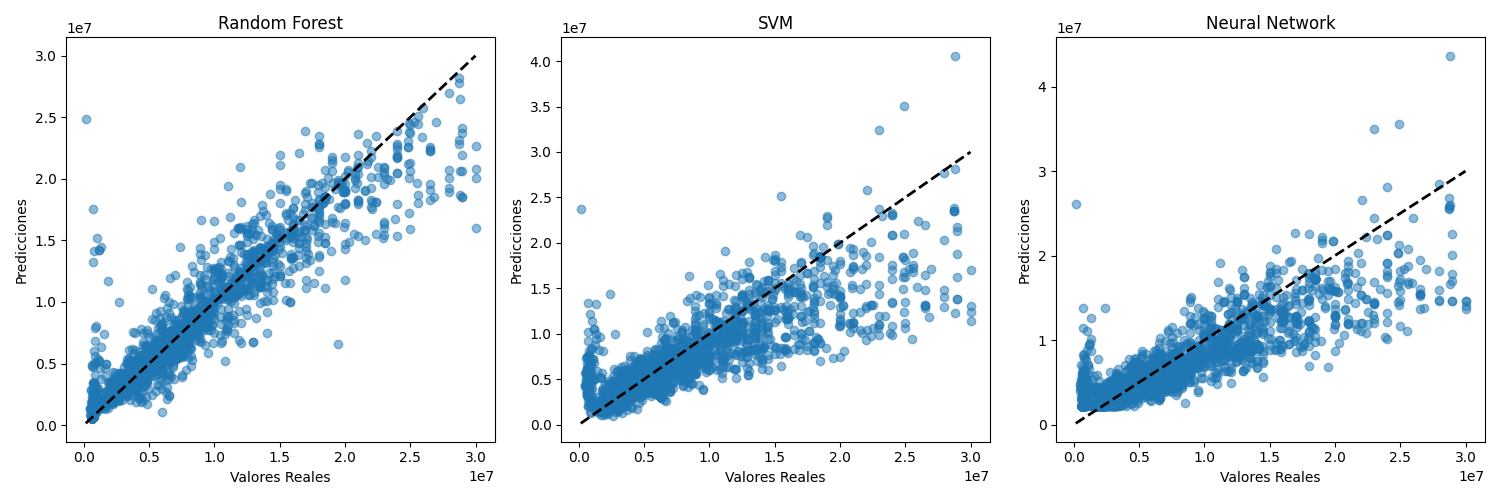
\includegraphics[width=0.8\textwidth]{imagenes/05-implementacion/servicio-web/plots.png}
    \caption{Gráfica de evaluación de los modelos de aprendizaje automático.}
    \label{fig:graficas-evaluacion}
\end{figure}

\subsection{API REST}
El servicio web exponer cuatro rutas principales, las cuales permiten a la
interfaz gráfica interactuar con los modelos de aprendizaje automático y obtener
información relevante sobre los mismos. Además, FastAPI permite documentar la API
de manera automática, lo que facilita la comprensión y el uso de la misma.

En el listado \ref{lst:api-rest} se muestra el código relevante para la
inicialización del servicio, la configuración de CORS y la definición de los modelos
que se utilizarán en la API para que FastAPI pueda generar la documentación de la
API de manera automática.

\begin{lstlisting}[language=python, caption={API REST}, label={lst:api-rest}]
# Inicialización de la aplicación
app = FastAPI(title="SkyPrice API",
                description="Hola, bienvenido a la API de **SkyPrice**. Aquí puedes predecir el precio de una propiedad utilizando tres modelos de aprendizaje automático: Random Forest, SVM y Redes Neuronales. Para predecir el precio de una propiedad, envía una solicitud POST a la ruta /predict con los datos de la propiedad. También puedes obtener información sobre los modelos y sus características en la ruta /models. ¡Diviértete!",
                version="1.0.0",
                docs_url="/openapi",
                openapi_url="/openapi.json",
                redoc_url="/redoc",
                summary="API para predecir el precio de un departamento en la CDMX",
                contact={
                    "name": "Humberto Alejandro Ortega Alcocer",
                    "email": "hortegaa1500@alumno.ipn.mx",
                    "url": "https://humbertowoody.xyz",
                },
                license_info={
                    "name": "MIT",
                    "url": "https://opensource.org/licenses/MIT",
                },
                terms_of_service="https://opensource.org/licenses/MIT",
                servers=[
                    {
                        "url": f"{HOSTNAME}",
                        "description": "URL de la API"
                    }
                ]
            )

# Configuración de CORS
app.add_middleware(
    CORSMiddleware,
    allow_credentials=True,
    allow_origins=["*"],
    allow_methods=["*"],
    allow_headers=["*"],
)

# Definición de una propiedad
class Property(BaseModel):
    Size_Terrain: float = Field(..., examples=[120.5], description="El tamaño del terreno en metros cuadrados")
    Size_Construction: float = Field(..., examples=[250.0], description="El tamaño de la construcción en metros cuadrados")
    Rooms: int = Field(..., examples=[3], description="El número de habitaciones")
    Bathrooms: float = Field(..., examples=[2.5], description="El número de baños")
    Parking: int = Field(..., examples=[1], description="El número de espacios de estacionamiento disponibles")
    Age: int = Field(..., examples=[5], description="La edad de la propiedad en años")
    Lat: float = Field(..., examples=[19.432608], description="La latitud de la propiedad")
    Lng: float = Field(..., examples=[-99.133209], description="La longitud de la propiedad")
    Municipality: str = Field(..., examples=["Benito Juárez"], description="El municipio donde se encuentra la propiedad")

# Definición de la respuesta del endpoint principal
class PrincipalResponse(BaseModel):
    message: str = Field(..., examples=["Bienvenido a la API de predicción inmobiliaria"], description="Mensaje de bienvenida")
    time: datetime.datetime = Field(..., examples=[datetime.datetime.now()], description="La hora actual del servidor")
    version: str = Field(..., examples=["0.1"], description="La versión de la API")
    description: str = Field(..., examples=["API para predecir el precio de una propiedad"], description="Descripción de la API")
    openapi: str = Field(..., examples=[f"{HOSTNAME}/openapi"], description="Enlace a la documentación de la API")
    redoc: str = Field(..., examples=[f"{HOSTNAME}/redoc"], description="Enlace a la documentación de la API en formato ReDoc")

# Definición de la respuesta del endpoint de predicciones
class PredictResponse(BaseModel):
    random_forest: float = Field(..., examples=[2500000.0], description="La predicción del precio de la propiedad con el modelo Random Forest")
    svm: float = Field(..., examples=[2700000.0], description="La predicción del precio de la propiedad con el modelo SVM")
    neural_network: float = Field(..., examples=[2600000.0], description="La predicción del precio de la propiedad con el modelo de Redes Neuronales")

# Definición de la respuesta del endpoint de modelos
class ModelsResponse(BaseModel):
    dataset: dict = Field(..., examples=[{"original": (1000,8),"training": {"X": (1000, 8), "y": (1000, 1)}, "testing": {"X": (250, 8), "y": (250, 1)}}], description="Información sobre los datos de entrenamiento y prueba")
    models: dict = Field(..., examples=[{"random_forest": {"mse": 1000000000.0, "ci": (900000000.0, 1100000000.0), "mae": 30000.0, "r2": 0.9, "feature_importances": [0.1, 0.2, 0.3, 0.4, 0.0, 0.0, 0.0, 0.0], "max_features": "auto", "max_depth": 10, "n_estimators": 100, "oob_score": True}, "svm": {"mse": 1500000000.0, "ci": (1400000000.0, 1600000000.0), "mae": 40000.0, "r2": 0.8, "kernel": "rbf", "C": 1.0, "epsilon": 0.1}, "neural_network": {"mse": 2000000000.0, "ci": (1900000000.0, 2100000000.0), "mae": 50000.0, "r2": 0.7, "learning_rate": 0.001, "beta_1": 0.9, "beta_2": 0.999, "epsilon": 1e-07}}], description="Información sobre los modelos y sus características")
\end{lstlisting}

\subsubsection{Ruta principal}
La ruta principal de la API REST proporciona información general sobre el servicio,
incluyendo la versión, la descripción, la hora actual del servidor y enlaces a
la documentación de la API en formato OpenAPI y ReDoc. En el listado \ref{lst:ruta-principal}
se muestra el código relevante para la ruta principal.

\begin{lstlisting}[language=python, caption={Ruta principal}, label={lst:ruta-principal}]
# Ruta principal
@app.get("/", summary="Ruta principal", description="Ruta principal de la API de predicción inmobiliaria.", tags=["Principal"], response_description="Mensaje de bienvenida", response_model=PrincipalResponse)
async def principal():
    # Regresamos un mensaje de bienvenida, la hora actual del servidor, la fecha, la versión del API, la descripción y un link a los docs de swagger.
    return {"message": "Bienvenido a la API de SkyPrice",
            "time": datetime.datetime.now(),
            "version": "1.0.0",
            "description": "API para predecir el precio de un departamento en la Ciudad de México, si deseas ver la documentación de la API, visita el enlace de OpenAPI (Swagger UI) o ReDoc:",
            "openapi": f"{HOSTNAME}/openapi",
            "redoc": f"{HOSTNAME}/redoc"}
\end{lstlisting}

En la figura \ref{fig:api-principal} se muestra la documentación de la API generada
para la ruta principal utilizando Swagger UI:

\begin{figure}[H]
    \centering
    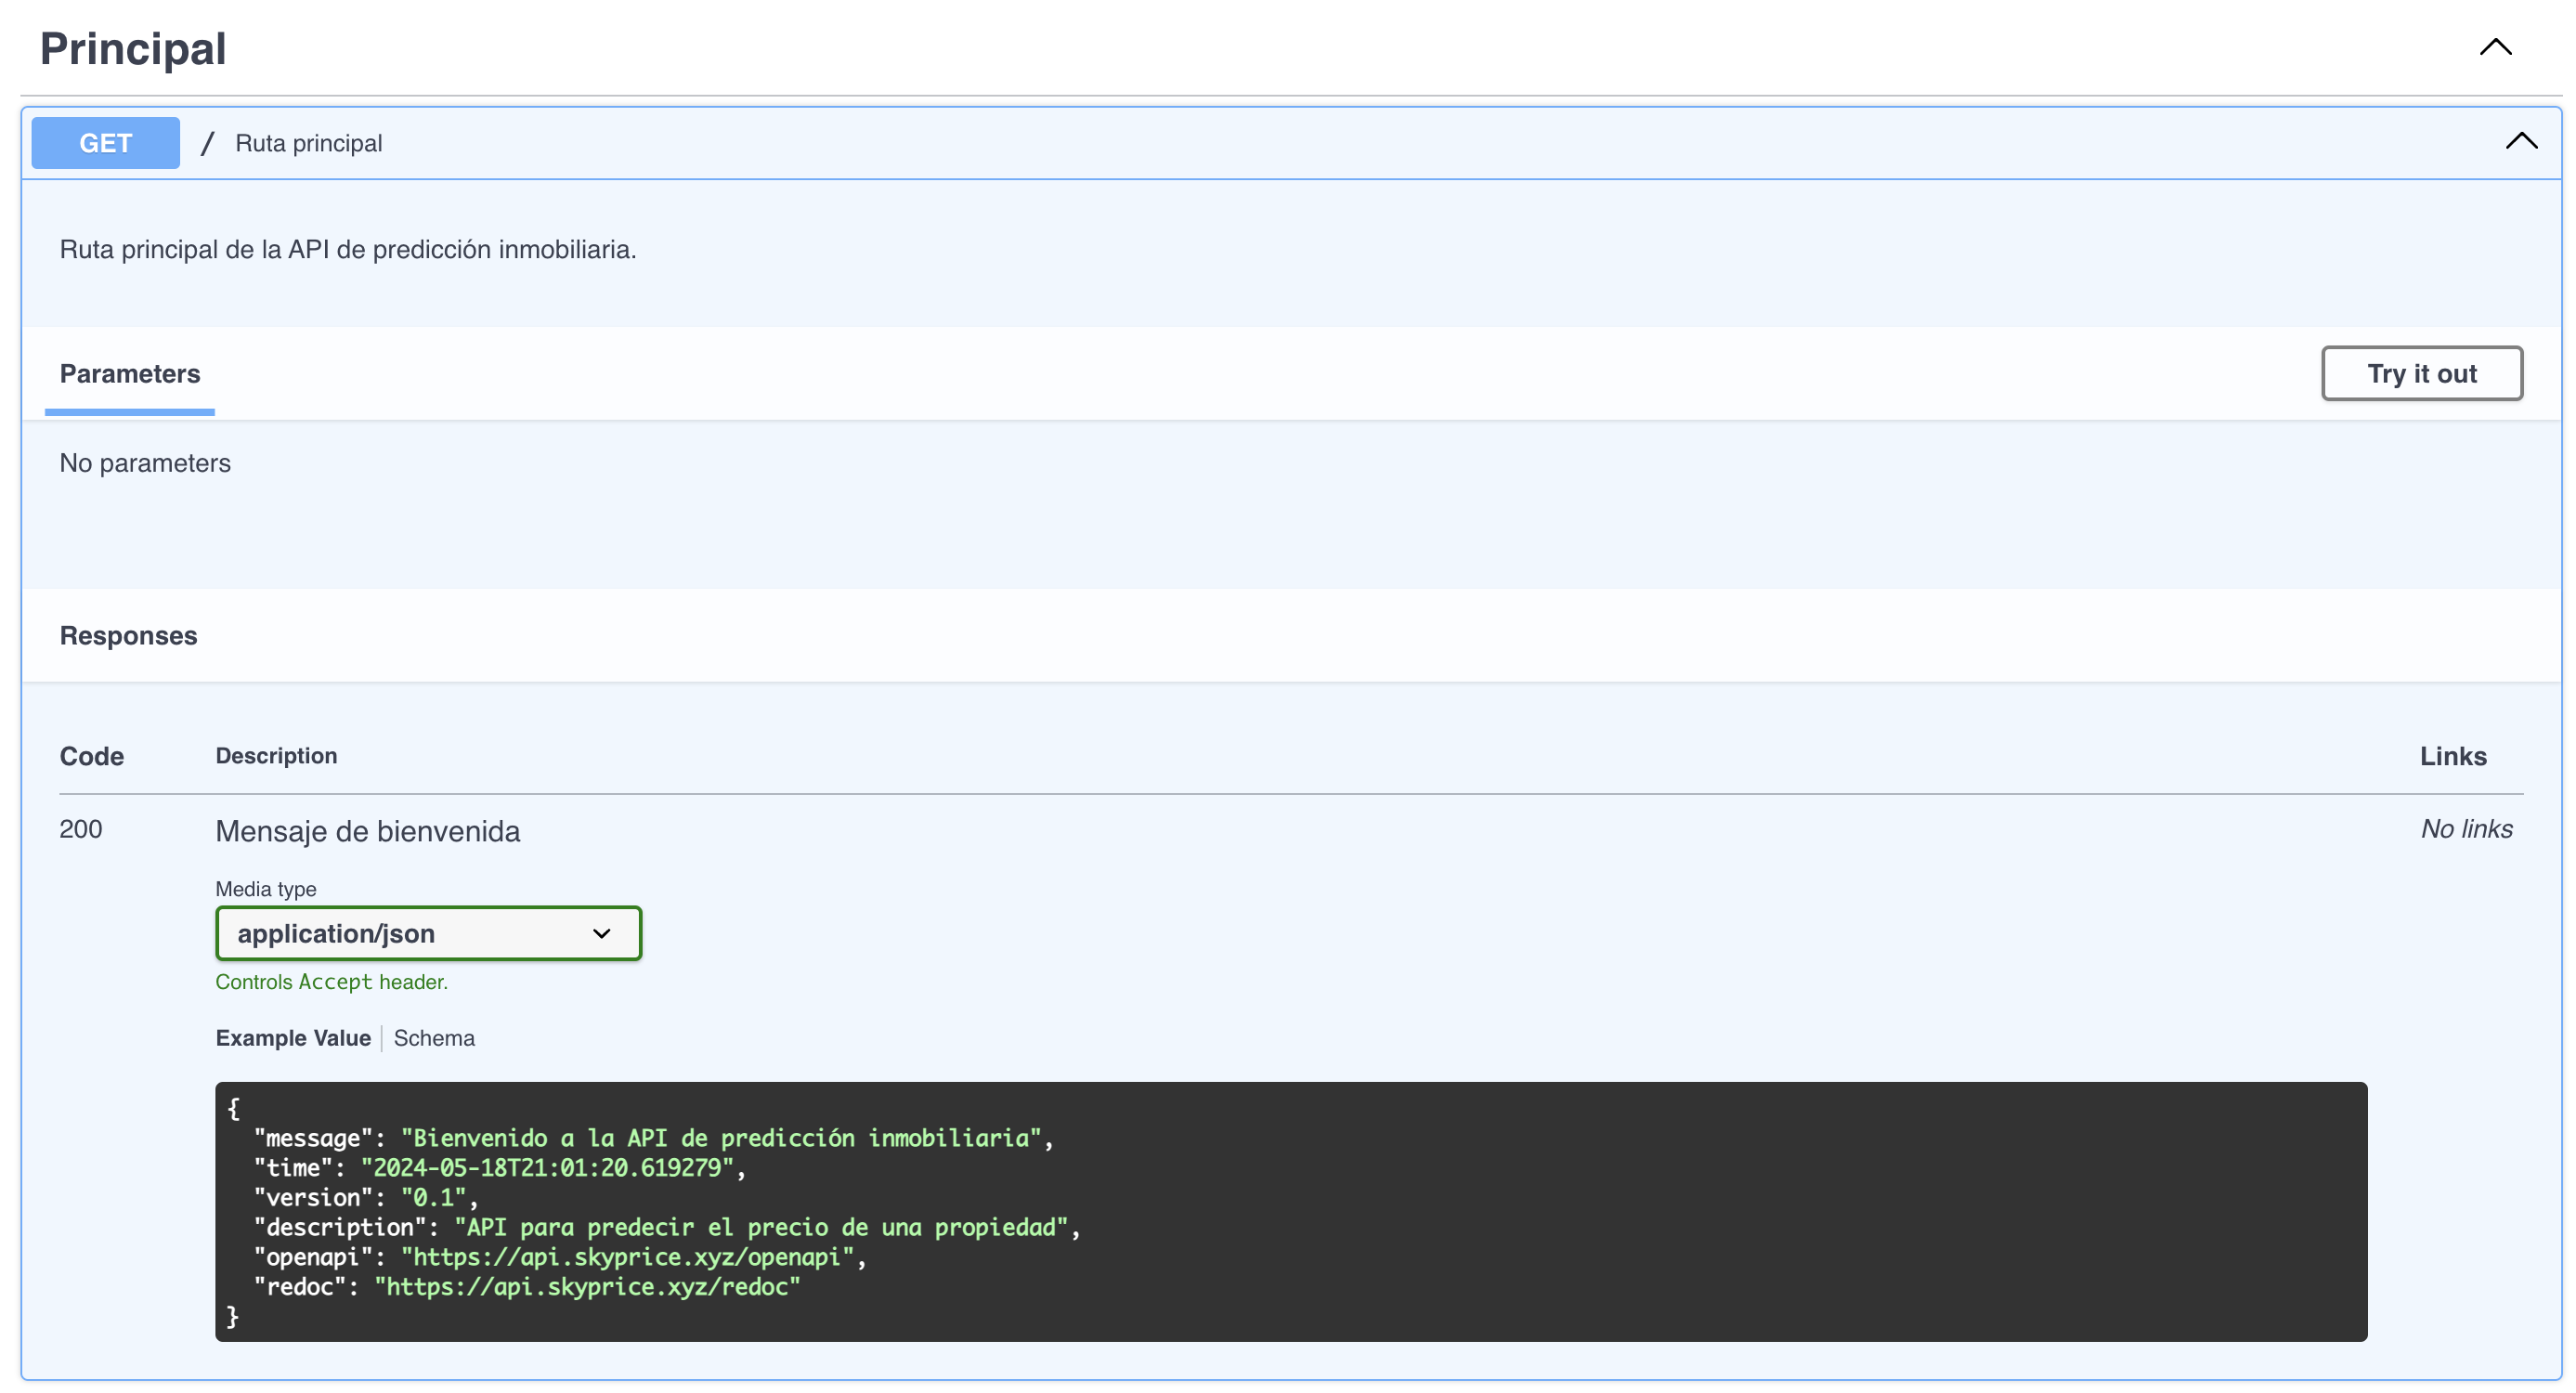
\includegraphics[width=1.0\textwidth]{imagenes/05-implementacion/servicio-web/api-principal.png}
    \caption{Documentación de la API para la ruta principal.}
    \label{fig:api-principal}
\end{figure}

\subsubsection{Ruta de predicción}
La ruta de predicción permite a los usuarios enviar datos sobre una propiedad
y obtener una estimación del precio utilizando los modelos de Random Forest,
Máquinas de Soporte Vectorial y Redes Neuronales. En el listado \ref{lst:ruta-prediccion}
se muestra el código relevante para la ruta de predicción.

\begin{lstlisting}[language=python, caption={Ruta de predicción}, label={lst:ruta-prediccion}]
# Ruta para predecir el precio de una propiedad
@app.post("/predict", summary="Predecir el precio de una propiedad", description="Predecir el precio de una propiedad utilizando tres modelos de aprendizaje automático: Random Forest, SVM y Redes Neuronales.", tags=["Predicciones"], response_description="Predicciones del precio de la propiedad", response_model=PredictResponse)
async def predict(property: Property):
    # Convertir entrada a DataFrame para preprocesamiento
    input_data = [property.Municipality, property.Size_Terrain, property.Size_Construction, property.Rooms, property.Bathrooms, property.Parking, property.Age, property.Lat, property.Lng]
    input_df = pd.DataFrame([input_data], columns=['Municipality', 'Size_Terrain', 'Size_Construction', 'Rooms', 'Bathrooms', 'Parking', 'Age', 'Lat', 'Lng'])

    # Predecir con cada modelo
    rf_pred,   = rf_model.predict(input_df)
    svm_pred = svm_model.predict(input_df)[0]
    # Preprocesar para la red neuronal y luego predecir
    nn_input = preprocessor.transform(input_df)
    nn_pred = nn_model.predict(nn_input)[0][0]

    # Devolver las predicciones
    return {
        "random_forest": float(rf_pred),
        "svm": float(svm_pred),
        "neural_network": float(nn_pred)
    }
\end{lstlisting}

En la figura \ref{fig:api-prediccion} se muestra la documentación de la API generada
para la ruta de predicción utilizando Swagger UI:

\begin{figure}[H]
    \centering
    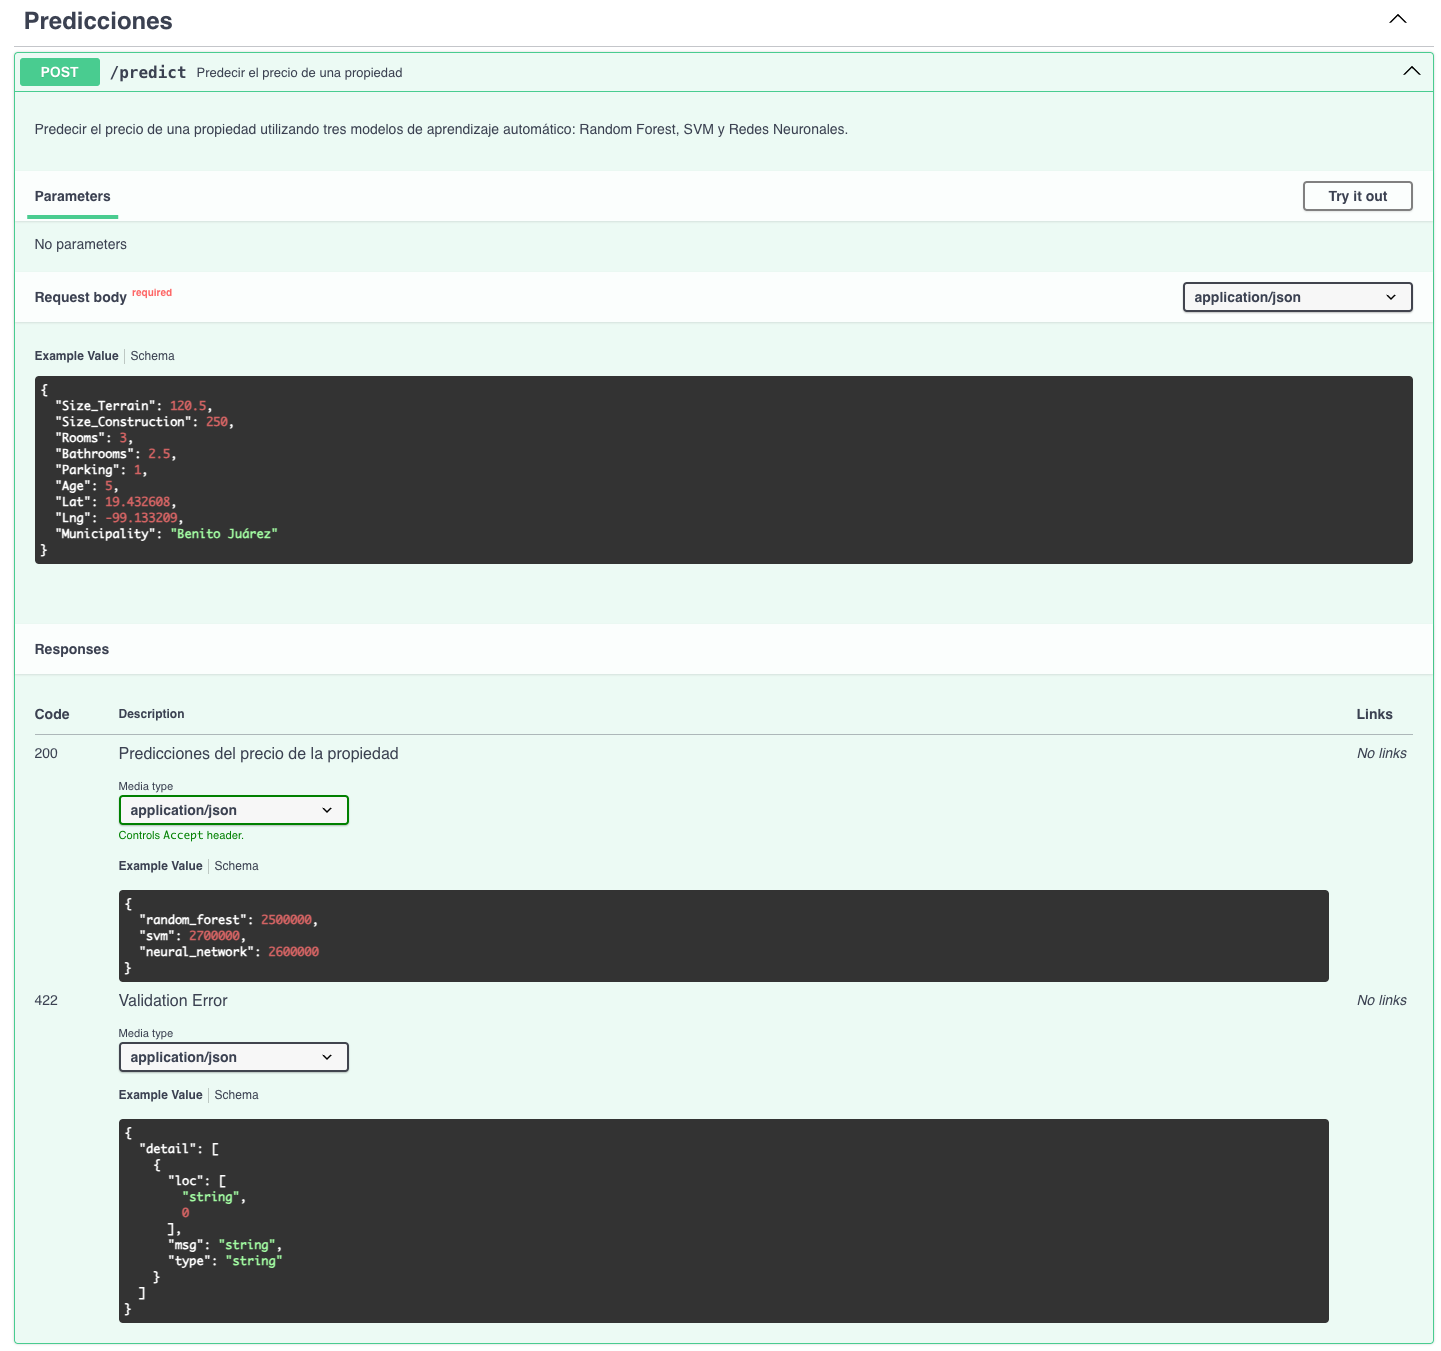
\includegraphics[width=1.0\textwidth]{imagenes/05-implementacion/servicio-web/api-prediccion.png}
    \caption{Documentación de la API para la ruta de predicción.}
    \label{fig:api-prediccion}
\end{figure}

\subsubsection{Ruta de gráficas de evaluación}
La ruta de gráficas de evaluación permite a los usuarios visualizar las predicciones
de los modelos de Random Forest, Máquinas de Soporte Vectorial y Redes Neuronales
en comparación con los valores reales. En el listado \ref{lst:ruta-graficas} se muestra
el código relevante para la ruta de gráficas de evaluación, destacando el uso de la
función \texttt{FileResponse} para servir archivos estáticos.

\begin{lstlisting}[language=python, caption={Ruta de gráficas de evaluación}, label={lst:ruta-graficas}]
# Ruta para obtener las gráficas de predicciones vs valores reales
@app.get("/plots", response_class=FileResponse, summary="Obtener gráficas de predicciones vs valores reales", description="Obtener las gráficas de predicciones vs valores reales de los modelos Random Forest, SVM y Redes Neuronales.", tags=["Gráficas"], response_description="Gráficas de predicciones vs valores reales")
async def plots():
        return FileResponse('plots.png')
\end{lstlisting}

En la figura \ref{fig:api-graficas} se muestra la documentación de la API generada
para la ruta de gráficas de evaluación utilizando Swagger UI:

\begin{figure}[H]
    \centering
    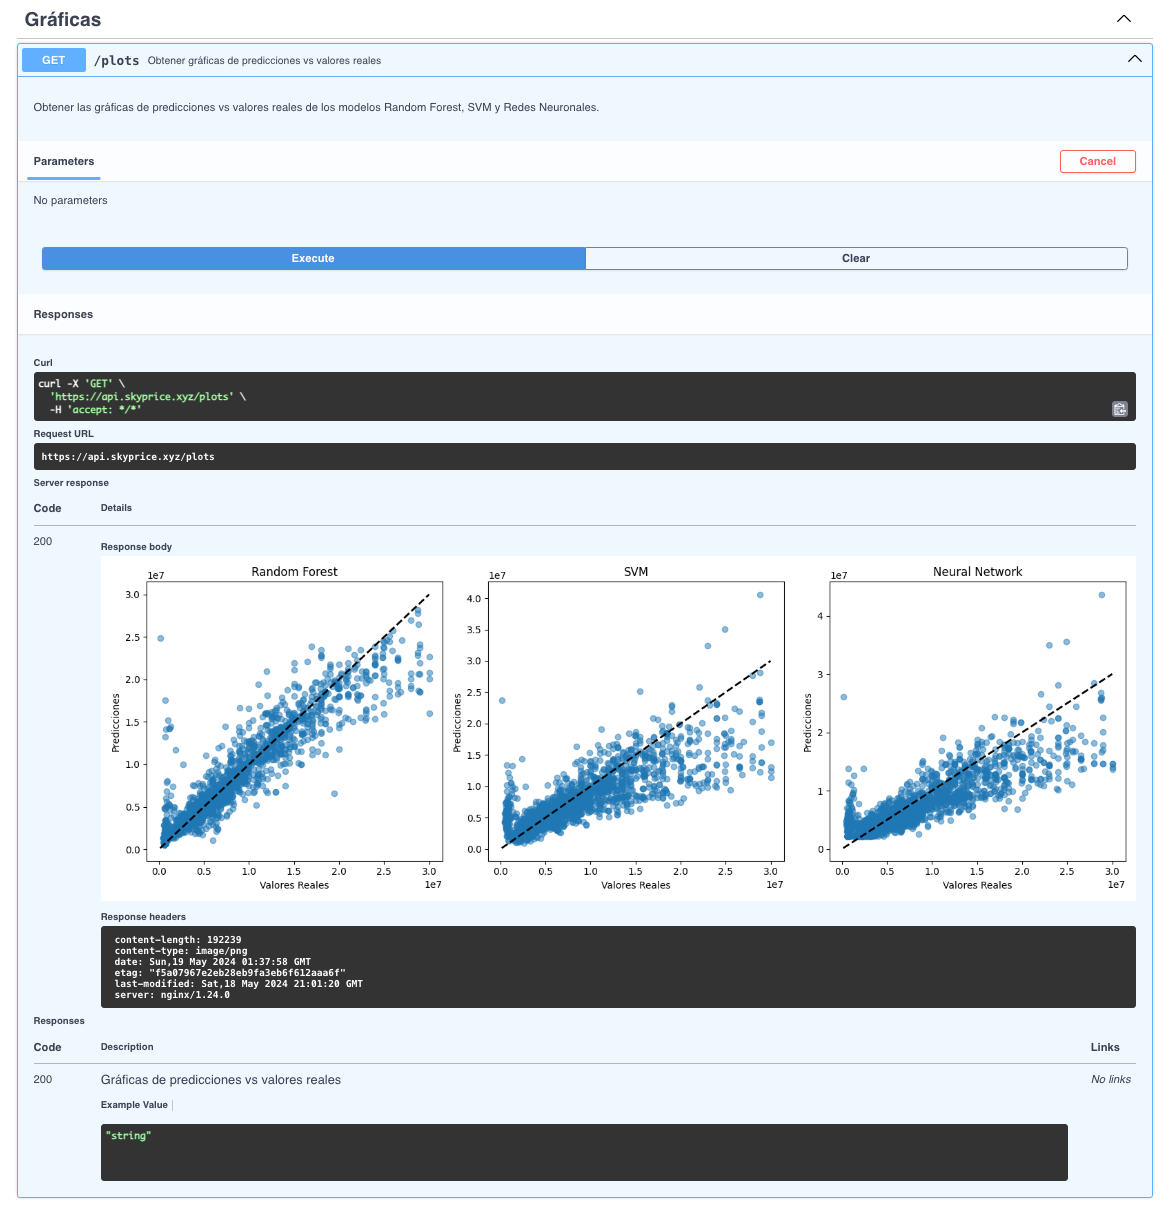
\includegraphics[width=1.0\textwidth]{imagenes/05-implementacion/servicio-web/api-plots.png}
    \caption{Documentación de la API para la ruta de gráficas de evaluación.}
    \label{fig:api-graficas}
\end{figure}

\subsubsection{Ruta de información de modelos}
La ruta de información de modelos permite a los usuarios obtener información detallada
sobre los modelos de Random Forest, Máquinas de Soporte Vectorial y Redes Neuronales,
incluyendo métricas de evaluación, hiperparámetros y características importantes. En el
listado \ref{lst:ruta-modelos} se muestra el código relevante para la ruta de información
de modelos.

\begin{lstlisting}[language=python, caption={Ruta de información de modelos}, label={lst:ruta-modelos}]
# Ruta para listar los modelos y sus características (ajuste de datos de entrenamiento, hiperparámetros, etc.)
@app.get("/models", summary="Obtener información sobre los modelos y sus características", description="Obtener información sobre los modelos de aprendizaje automático utilizados en la API, incluyendo sus características, ajuste de datos de entrenamiento, hiperparámetros, etc.", tags=["Modelos"], response_description="Información sobre los modelos y sus características", response_model=ModelsResponse)
async def models_info():
    # Regresar información sobre los modelos y sus características
    return {
        "dataset": {
            "original": df.shape,
            "training": {
                "X": X_train.shape,
                "y": y_train.shape
            },
            "testing": {
                "X": X_test.shape,
                "y": y_test.shape
            }
        },
        "models":{
            "random_forest": {
                "mse": rf_mse,
                "rmse": rf_rmse,
                "ci": rf_ci,
                "mae": rf_mae,
                "r2": rf_r2 ,
                "feature_importances": rf_model['regressor'].feature_importances_.tolist(),
                "max_features": rf_model['regressor'].max_features,
                "max_depth": rf_model['regressor'].max_depth,
                "n_estimators": rf_model['regressor'].n_estimators,
                "oob_score": rf_model['regressor'].oob_score,
            },
            "svm": {
                "mse": svm_mse,
                "rmse": svm_rmse,
                "ci": svm_ci,
                "mae": svm_mae,
                "r2": svm_r2,
                "kernel": svm_model['svr'].kernel,
                "C": svm_model['svr'].C,
                "epsilon": svm_model['svr'].epsilon
            },
            "neural_network": {
                "mse": nn_mse,
                "rmse": nn_rmse,
                "ci": nn_ci,
                "mae": nn_mae,
                "r2": nn_r2,
                "learning_rate": float(nn_model.optimizer.learning_rate.numpy()),
                "beta_1": nn_model.optimizer.beta_1,
                "beta_2": nn_model.optimizer.beta_2,
                "epsilon": nn_model.optimizer.epsilon
            }
        }
    }
\end{lstlisting}

En la figura \ref{fig:api-modelos} se muestra la documentación de la API generada
para la ruta de información de modelos utilizando Swagger UI:

\begin{figure}[H]
    \centering
    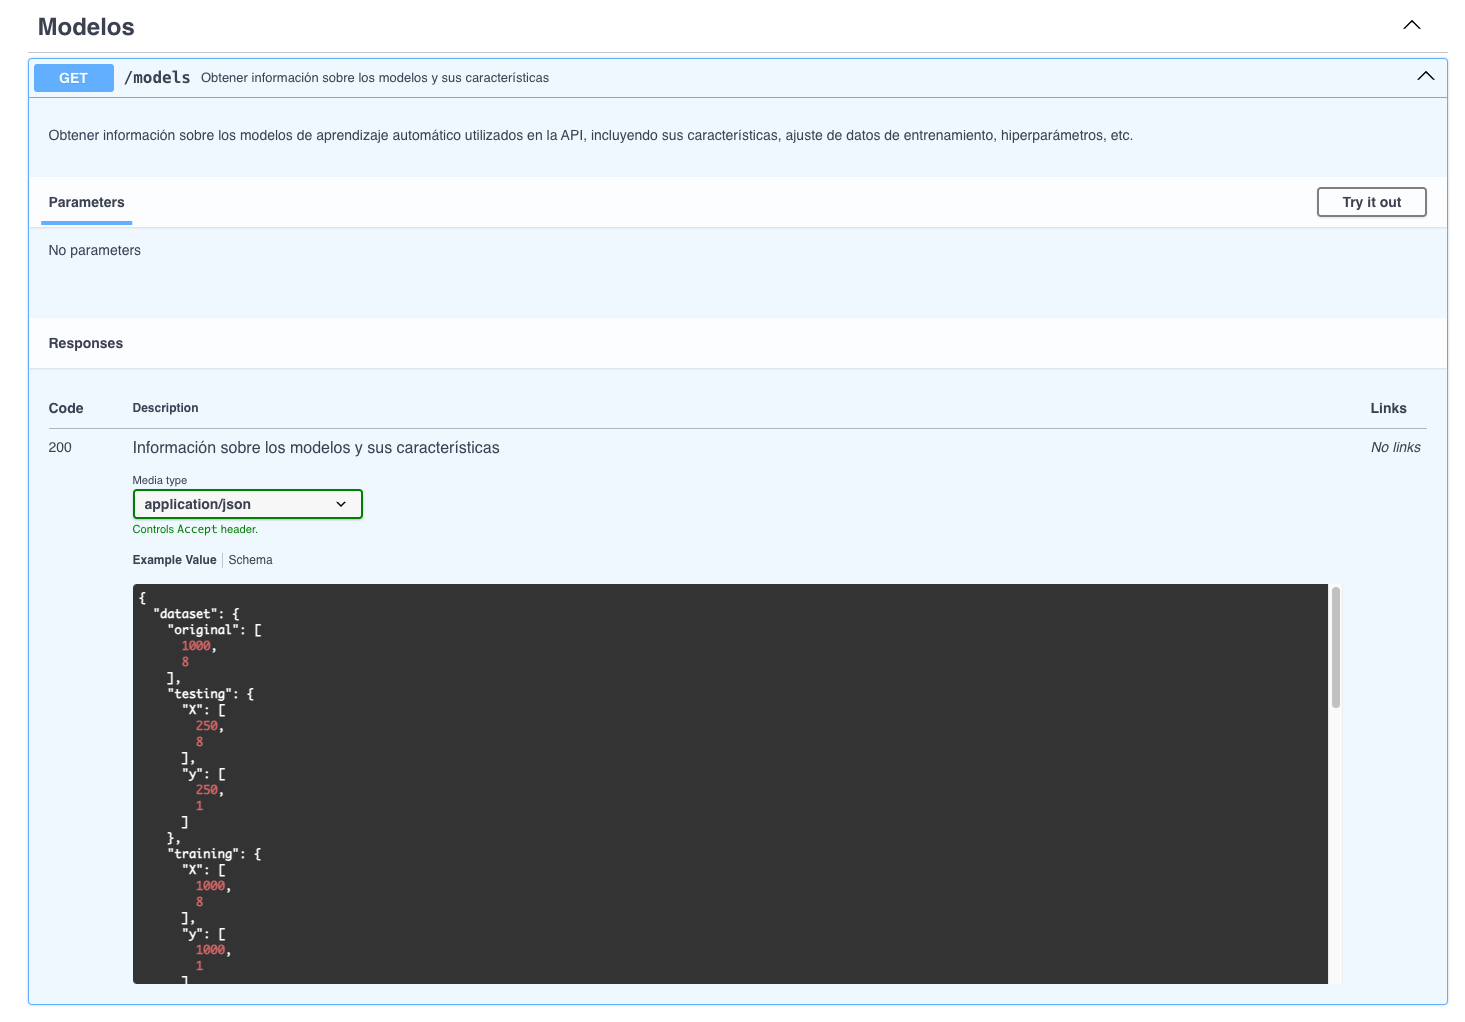
\includegraphics[width=1.0\textwidth]{imagenes/05-implementacion/servicio-web/api-models.png}
    \caption{Documentación de la API para la ruta de información de modelos.}
    \label{fig:api-modelos}
\end{figure}

\subsection{Documentación}
FastAPI permite documentar la API de manera automática utilizando la información
proporcionada en las rutas y modelos definidos. La documentación se genera en
formato OpenAPI (Swagger) y ReDoc, lo que facilita la comprensión y el uso de la API.

Esta documentación no solo es útil para el desarrollo de la interfaz gráfica en
el actual trabajo terminal, sino que también es útil para otros desarrolladores
que deseen integrar la API en sus propios proyectos.

\subsubsection{OpenAPI (Swagger)}
La documentación de la API en formato OpenAPI (Swagger) permite a los usuarios
explorar los endpoints, los modelos y los parámetros de la API de manera interactiva.
En la figura \ref{fig:skyprice-openapi} se muestra la documentación de la API en
formato OpenAPI, la cual incluye información detallada sobre los endpoints y los
modelos utilizados en la API.

\begin{figure}[H]
    \centering
    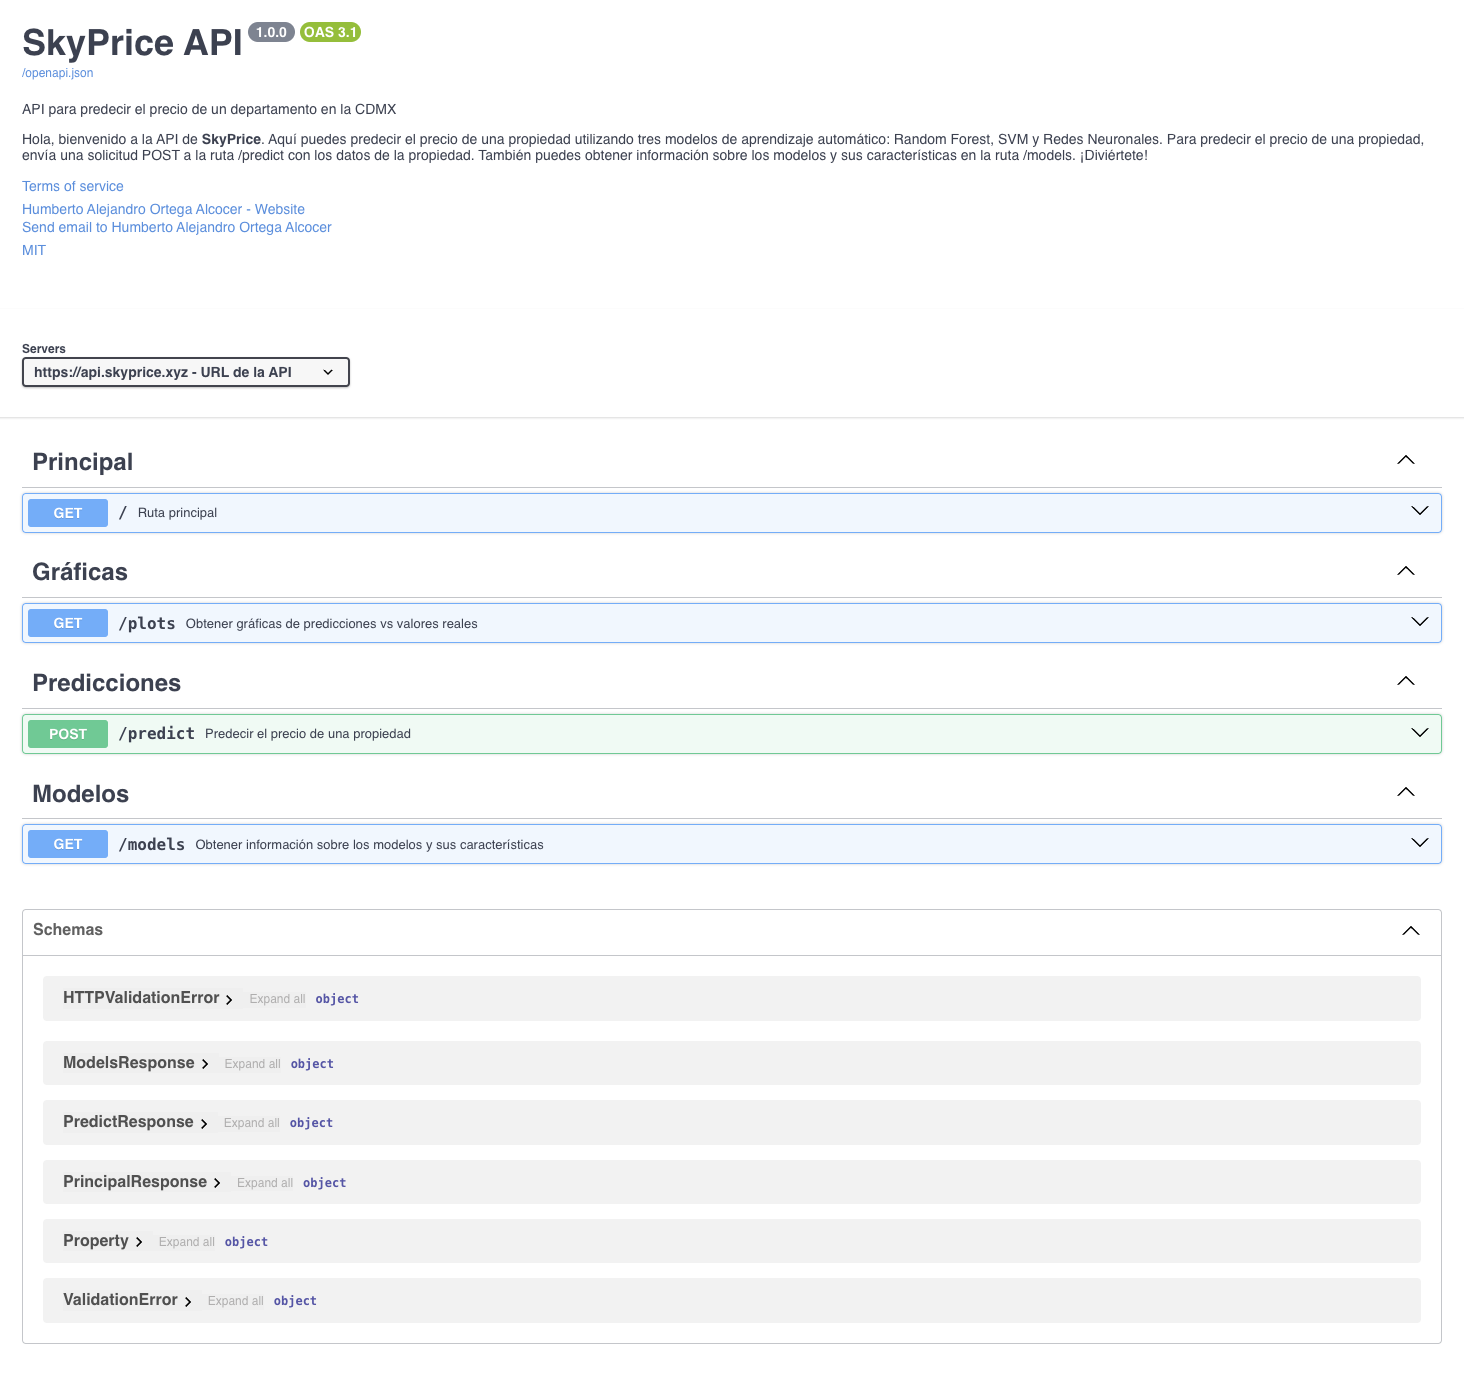
\includegraphics[width=0.8\textwidth]{imagenes/05-implementacion/servicio-web/openapi.png}
    \caption{Documentación de la API en formato OpenAPI (Swagger).}
    \label{fig:skyprice-openapi}
\end{figure}

\subsubsection{ReDoc}
La documentación de la API en formato ReDoc permite a los usuarios explorar los
endpoints, los modelos y los parámetros de la API de manera interactiva y visual,
además de proveer una interfaz de documentación más editorial y amigable. En la
figura \ref{fig:skyprice-redoc} se muestra la documentación de la API en formato
ReDoc.

\begin{figure}[H]
    \centering
    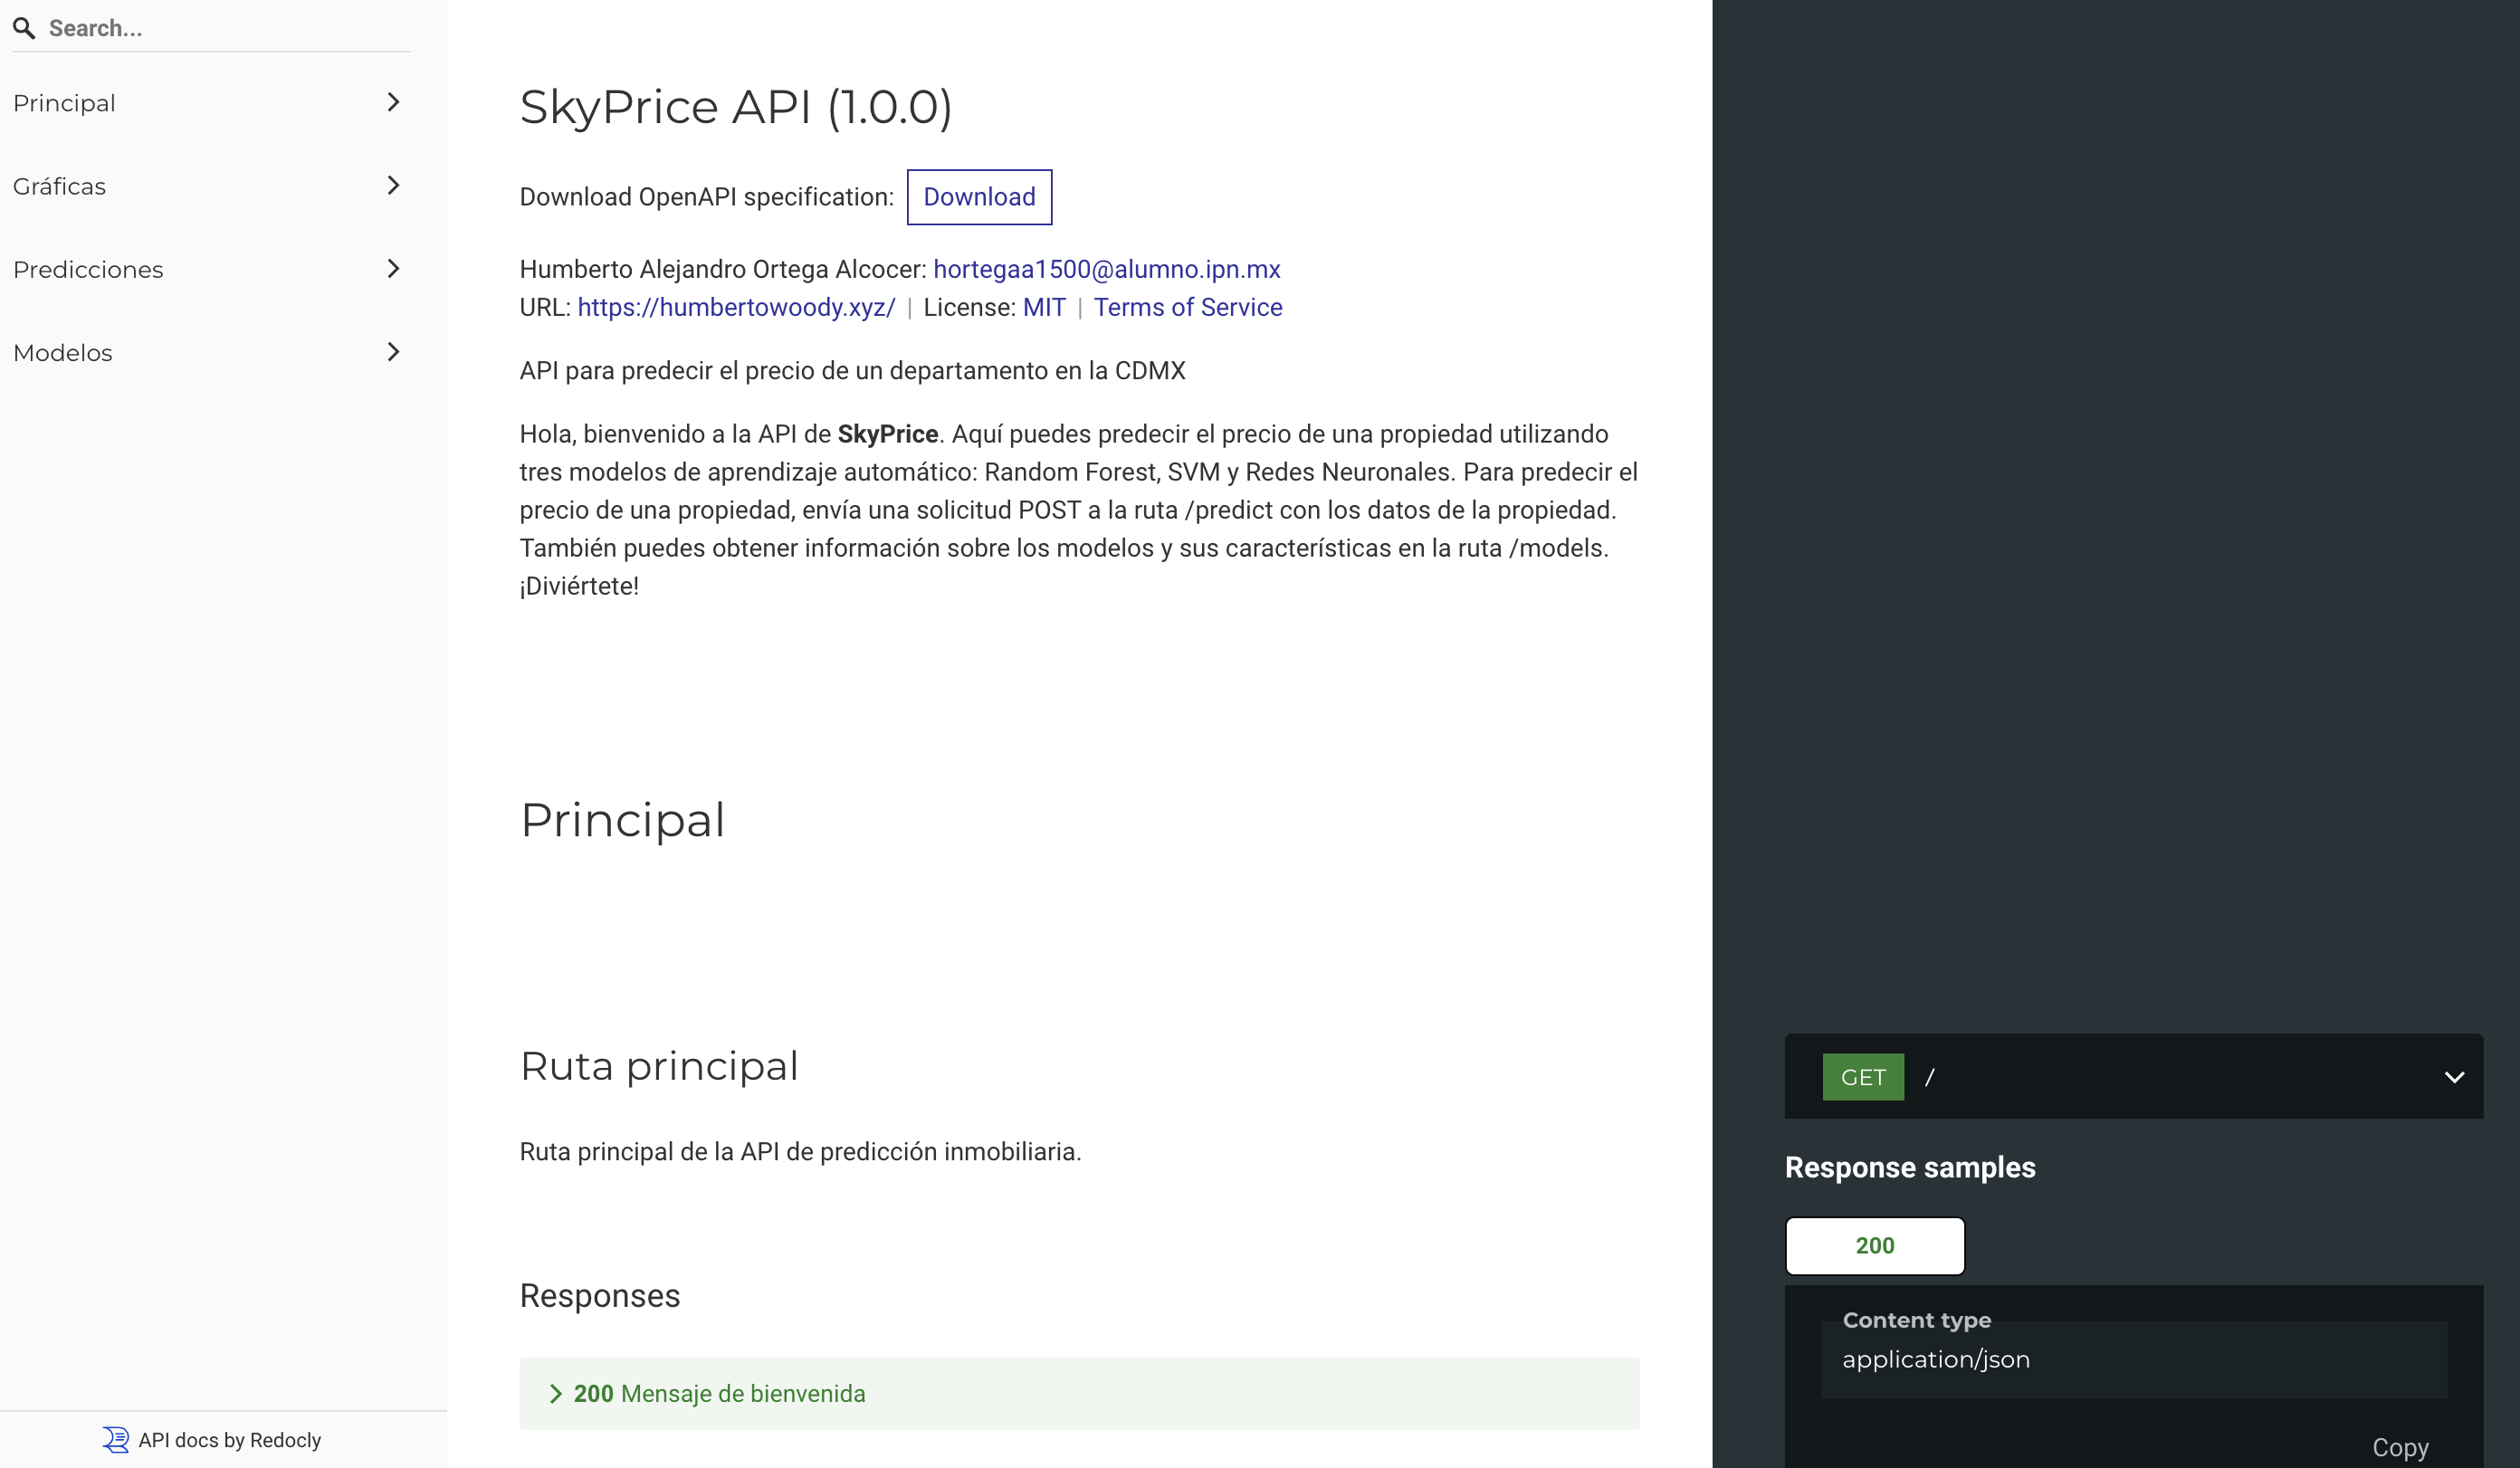
\includegraphics[width=0.6\textwidth]{imagenes/05-implementacion/servicio-web/redoc.png}
    \caption{Documentación de la API en formato ReDoc.}
    \label{fig:skyprice-redoc}
\end{figure}


\section{Interfaz gráfica}
La interfaz gráfica se implementó utilizando React con NextJS como marco de trabajo y
Material-UI como biblioteca de componentes. La interfaz gráfica permite a los
usuarios interactuar con los modelos de aprendizaje automático, obtener
información sobre los modelos y realizar predicciones de precio para propiedades
en la Ciudad de México, además se incluye un mapa interactivo con la ubicación de
las propiedades y otras capas de datos relevantes.

\subsection{Estructura del proyecto}
En la figura \ref{fig:estructura-proyecto} se muestra la estructura del proyecto
de la interfaz gráfica, la cual se divide en diferentes carpetas y archivos para
facilitar el desarrollo y el mantenimiento del código.

\begin{figure}[H]
    \centering
    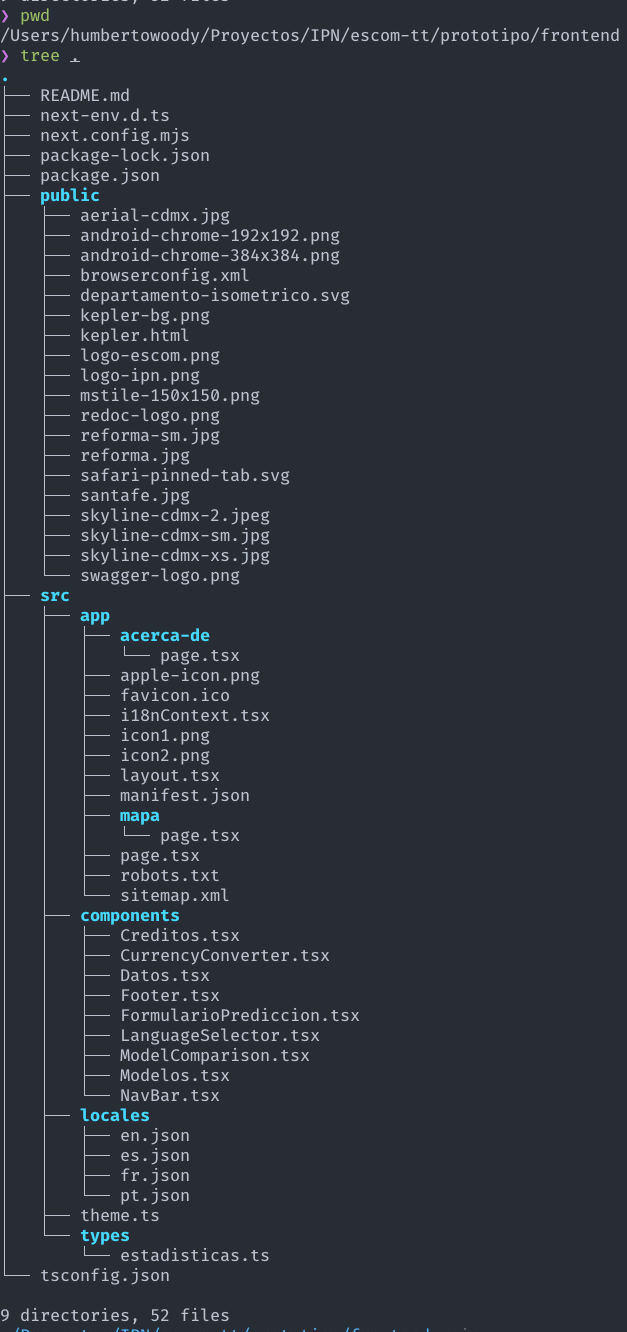
\includegraphics[width=0.8\textwidth]{imagenes/05-implementacion/interfaz-grafica/estructura-proyecto.png}
    \caption{Estructura del proyecto de la interfaz gráfica.}
    \label{fig:estructura-proyecto}
\end{figure}

\subsection{Navegación y traducciones}
La interfaz gráfica incluye un menú de navegación con enlaces a las diferentes
secciones de la página, como la sección de estimación de precio, la sección de
acerca de y el mapa interactivo. Además, se incluyó soporte para traducciones
en inglés, español, francés y portugués utilizando la biblioteca i18next. En la
estructura mostrada en la figura \ref{fig:estructura-proyecto} se puede observar
la carpeta \texttt{src/locales} que contiene los archivos de traducción para
cada idioma.

En la figura \ref{fig:frances} se muestra la interfaz gráfica en francés, la cual
incluye traducciones para los textos y los mensajes de la página.

\begin{figure}[H]
    \centering
    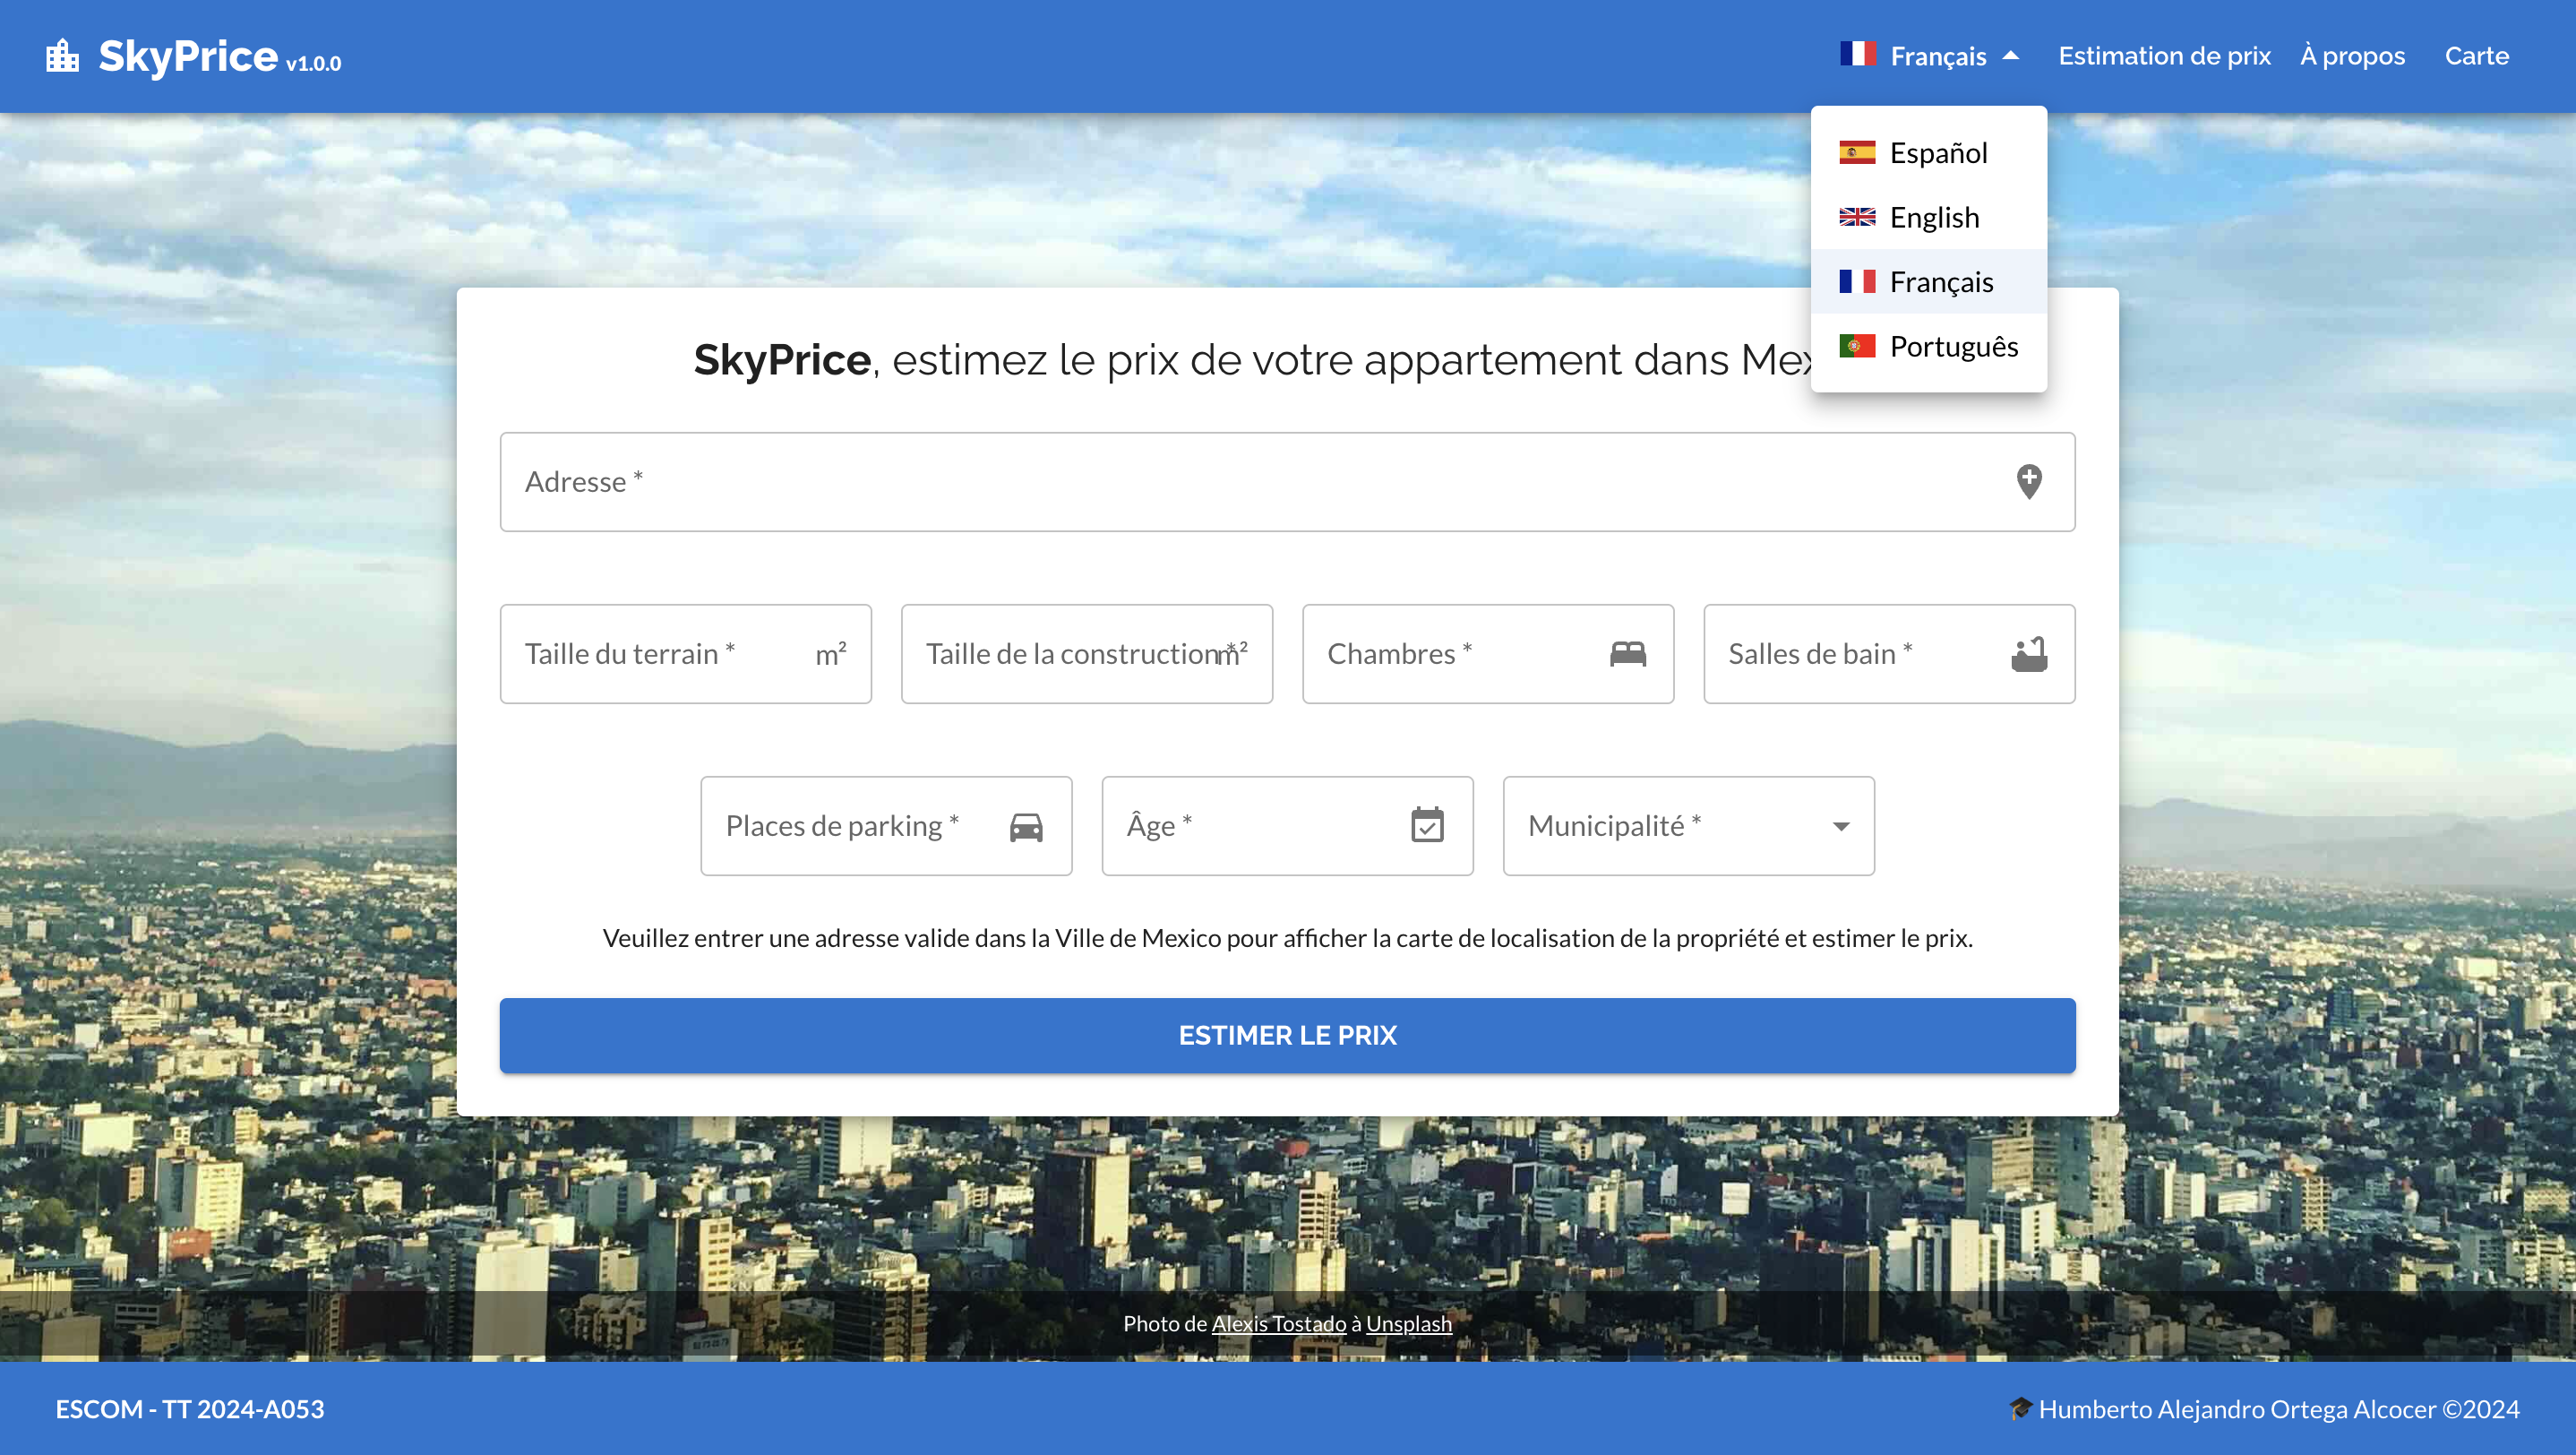
\includegraphics[width=1.0\textwidth]{imagenes/05-implementacion/interfaz-grafica/frances.png}
    \caption{Interfaz gráfica en francés.}
    \label{fig:frances}
\end{figure}

\subsubsection{Traducción de textos}
La traducción de textos se implementó utilizando la biblioteca i18next, la cual
permite definir archivos de traducción para cada idioma y utilizarlos en la interfaz
gráfica. En el listado \ref{lst:traduccion-textos} se muestra el código relevante
para la traducción de textos en la interfaz gráfica en una de las secciones.

\begin{lstlisting}[language=javascript, caption={Traducción de textos}, label={lst:traduccion-textos}]
const [lang, setLang] = useState<string>(defLang);
const [translations, setTranslations] = useState({ ...defTranslations });

useEffect(() => {
  import(`@/locales/${lang}.json`)
    .then((module) => {
      setTranslations(module.default);
      localStorage.setItem('i18nextLng', lang);
      console.info(`Traducciones cargadas para el idioma ${lang}`);
    })
    .catch(() => {
      console.error(
        `Archivo de traducciones no encontrado para el idioma ${lang}`,
      );
    });
}, [lang]);
\end{lstlisting}

Un ejemplo de archivo de traducción en inglés se muestra en el listado \ref{lst:ingles},
el cual muestra un fragmento de un archivo de traducción en inglés con los textos
utilizados en la interfaz gráfica.

\begin{lstlisting}[language=json, caption={Archivo de traducción en inglés}, label={lst:ingles}]
{
  "navbar": {
    "home": "Home",
    "prediction": "Prediction",
    "about": "About",
    "map": "Map"
  },
  "predictionForm": {
    "title": "Property Price Prediction",
    "subtitle": "Enter the property details to get an estimate of the price",
    "sizeTerrain": "Terrain Size (m^2)",
    "sizeConstruction": "Construction Size (m^2)",
    "rooms": "Rooms",
    "bathrooms": "Bathrooms",
    "parking": "Parking",
    "age": "Age",
    "lat": "Latitude",
    "lng": "Longitude",
    "municipality": "Municipality",
    "submit": "Predict"
  },
}
\end{lstlisting}

\subsection{Estimación de precio}
La página principal de la interfaz gráfica incluye una sección donde los usuarios
pueden ingresar datos sobre una propiedad y obtener una estimación del precio. Esta
funcionalidad consiste en un formulario con campos para los datos de la propiedad,
validación para dichos campos, y un botón para realizar la predicción. En la figura
\ref{fig:estimacion-precio} se muestra la sección de estimación de precio de la
interfaz gráfica.

\begin{figure}[H]
    \centering
    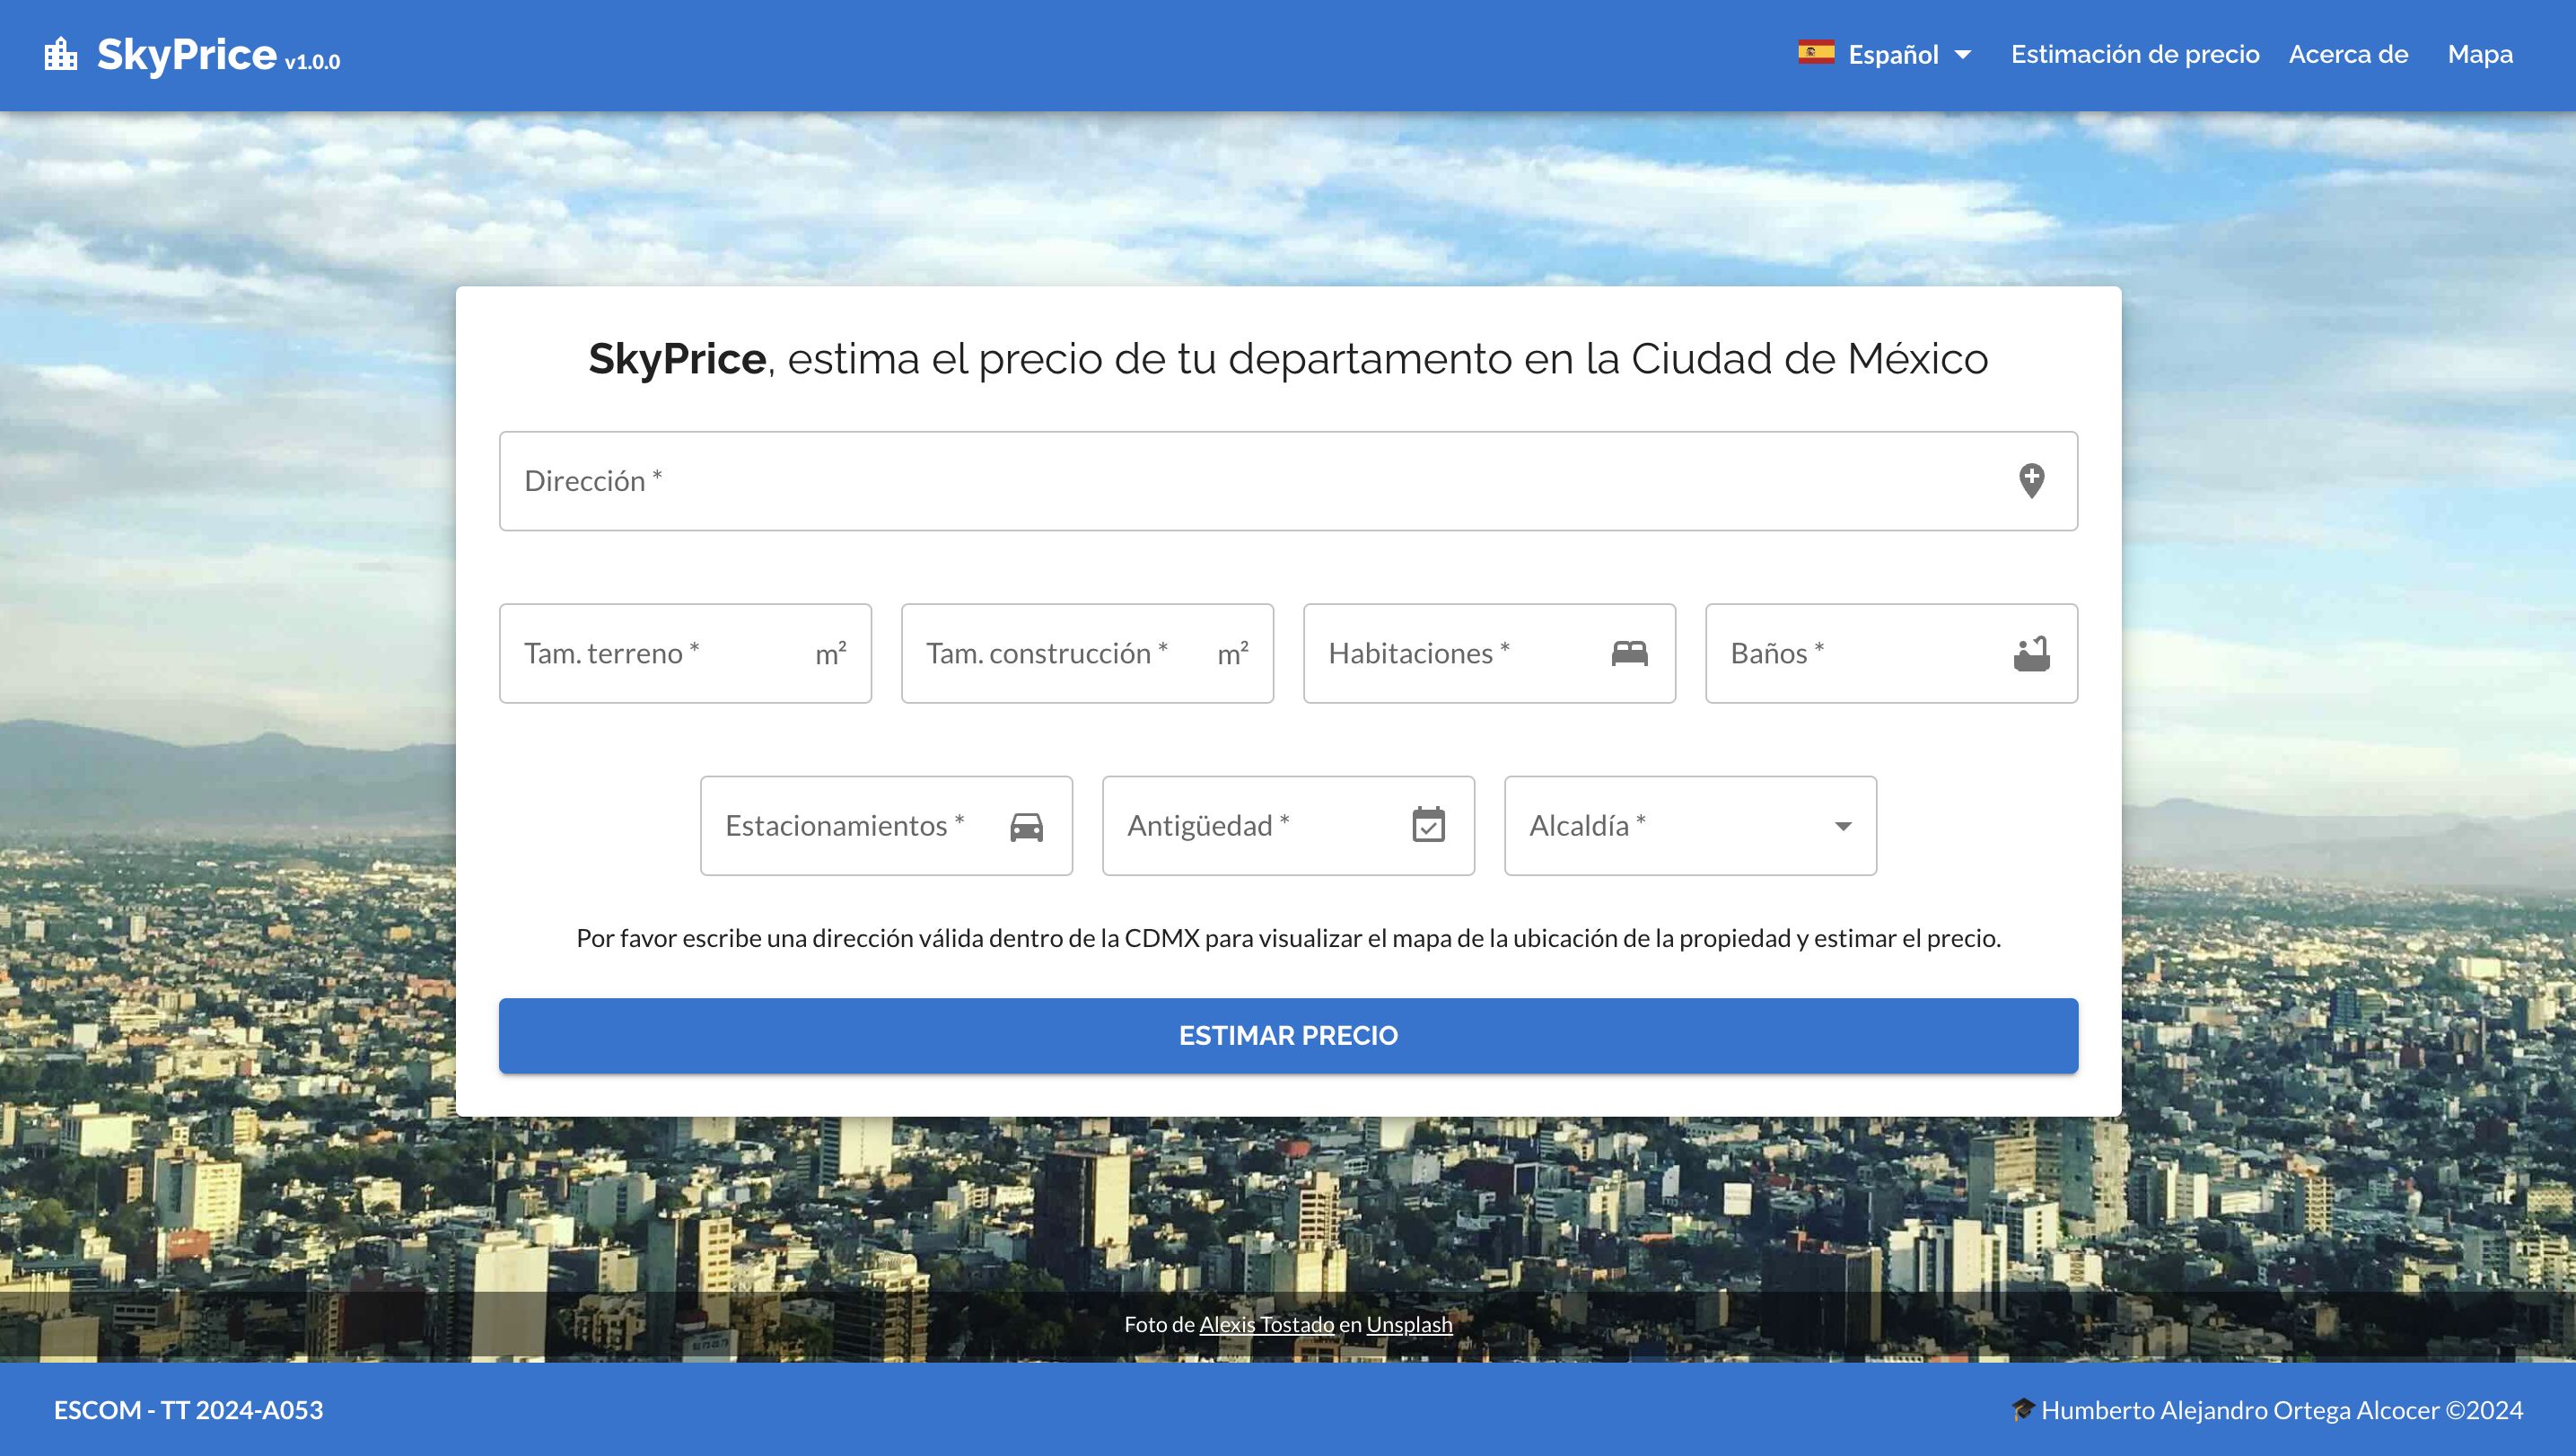
\includegraphics[width=1.0\textwidth]{imagenes/05-implementacion/interfaz-grafica/formulario-prediccion.png}
    \caption{Sección de estimación de precio de la interfaz gráfica.}
    \label{fig:estimacion-precio}
\end{figure}

\subsubsection{Validación de campos}
La validación de campos se implementó utilizando la biblioteca Yup, la cual permite
definir esquemas de validación para los campos del formulario. En el listado
\ref{lst:validacion-campos} se muestra el código relevante para la validación de
campos en la sección de estimación de precio.

\begin{lstlisting}[language=javascript, caption={Validación de campos}, label={lst:validacion-campos}]
  // Esquema de validación para el formulario
  const validationSchema = yup.object({
    Size_Terrain: yup
      .number()
      .required(t('predictionForm.validations.sizeTerrainRequired'))
      .min(10, t('predictionForm.validations.sizeTerrainMin', { min: 10 }))
      .max(1000, t('predictionForm.validations.sizeTerrainMax', { max: 1000 })),
    Size_Construction: yup
      .number()
      .required(t('predictionForm.validations.sizeConstructionRequired'))
      .min(10, t('predictionForm.validations.sizeConstructionMin', { min: 10 }))
      .max(
        1000,
        t('predictionForm.validations.sizeConstructionMax', { max: 1000 }),
      ),
    Rooms: yup
      .number()
      .required(t('predictionForm.validations.roomsRequired'))
      .integer()
      .min(0, t('predictionForm.validations.roomsMin', { min: 0 }))
      .max(10, t('predictionForm.validations.roomsMax', { max: 10 })),
    // Validar que los baños sean un número en pasos de 0.5 y mayor a 1 (mínimo 1 baño)
    Bathrooms: yup
      .number()
      .required(t('predictionForm.validations.bathroomsRequired'))
      .min(1, t('predictionForm.validations.bathroomsMin', { min: 1 }))
      .max(10, t('predictionForm.validations.bathroomsMax', { max: 10 }))
      .test(
        'is-half',
        t('predictionForm.validations.bathroomsHalf'),
        (value) => {
          if (value) {
            return value % 0.5 === 0;
          }
          return true;
        },
      ),
    Parking: yup
      .number()
      .required(t('predictionForm.validations.parkingRequired'))
      .integer()
      .min(0, t('predictionForm.validations.parkingMin', { min: 0 }))
      .max(5, t('predictionForm.validations.parkingMax', { max: 5 })),
    Age: yup
      .number()
      .required(t('predictionForm.validations.ageRequired'))
      .integer()
      .min(0, t('predictionForm.validations.ageMin', { min: 0 }))
      .max(100, t('predictionForm.validations.ageMax', { max: 100 })),
    Lat: yup
      .number()
      .required(t('predictionForm.validations.latRequired'))
      .min(19.1, t('predictionForm.validations.outOfBounds'))
      .max(19.7, t('predictionForm.validations.outOfBounds')),
    Lng: yup
      .number()
      .required(t('predictionForm.validations.lngRequired'))
      .min(-99.4, t('predictionForm.validations.outOfBounds'))
      .max(-98.9, t('predictionForm.validations.outOfBounds')),
    Municipality: yup
      .string()
      .required(t('predictionForm.validations.municipalityRequired'))
      .oneOf(alcaldias, t('predictionForm.validations.municipalityInvalid')),
  });
\end{lstlisting}

\subsubsection{Envío de datos}
El envío de datos se implementó utilizando \texttt{fetch} para realizar una petición
POST a la API REST con los datos de la propiedad. En el listado \ref{lst:envio-datos}
se muestra el código relevante para el envío de datos en la sección de estimación de
precio.

\begin{lstlisting}[language=javascript, caption={Envío de datos}, label={lst:envio-datos}]
// Función para enviar los datos de la propiedad a la API
const handleSubmit = async (values) => {
  try {
    // Realizar la petición POST a la API REST
    const response = await fetch(`${process.env.NEXT_PUBLIC_API_URL}/predict`, {
      method: 'POST',
      headers: {
        'Content-Type': 'application/json',
      },
      body: JSON.stringify(values),
    });

    // Verificar si la petición fue exitosa
    if (response.ok) {
      // Obtener los datos de la respuesta
      const data = await response.json();
      // Actualizar el estado con los datos de la predicción
      setPrediction(data);
    } else {
      // Mostrar un mensaje de error si la petición falla
      throw new Error('Error al realizar la predicción');
    }
  } catch (error) {
    // Mostrar un mensaje de error si la petición falla
    console.error(error);
  }
};
\end{lstlisting}

\subsubsection{Geocodificación}
Para realizar la geocodificación de la dirección proporcionada por el usuario, se
utilizó Google Maps API para obtener las coordenadas geográficas (latitud y longitud)
de la dirección. En el listado \ref{lst:geocodificacion} se muestra el código relevante
para la geocodificación en la sección de estimación de precio.

\begin{lstlisting}[language=javascript, caption={Geocodificación}, label={lst:geocodificacion}]
const onPlaceChanged = () => {
  if (autocomplete !== null) {
    // @ts-ignore
    const place = autocomplete.getPlace();
    if (!place) {
      console.warn('No se pudo obtener la información del lugar');
      return;
    }

    // Extraer latitud y longitud del lugar
    const lat = place?.geometry?.location?.lat();
    const lng = place?.geometry?.location?.lng();

    // Extrae el municipio del componente de dirección de place
    const municipality = encontrarMunicipio(
      place.address_components,
      place.formatted_address,
    );

    // Actualiza el estado del formulario con estos valores
    formik.setFieldValue('Lat', lat);
    formik.setFieldValue('Lng', lng);
    formik.setFieldValue('Municipality', municipality);

    // Actualizar el estado de la Dirección
    setAddress(place.formatted_address);
  } else {
    console.log('Autocomplete aún no está cargado');
  }
};
\end{lstlisting}

Una vez que el usuario ha introducido una dirección y se ha realizado la geocodificación,
se extrae el municipio de la dirección proporcionada (alcaldía) y se muestra
un mapa interactivo con la ubicación de la propiedad. En la figura \ref{fig:geocodificacion}
se muestra el formulario con datos de una propiedad así como el mapa resultante de la
geocodificación.

\begin{figure}[H]
    \centering
    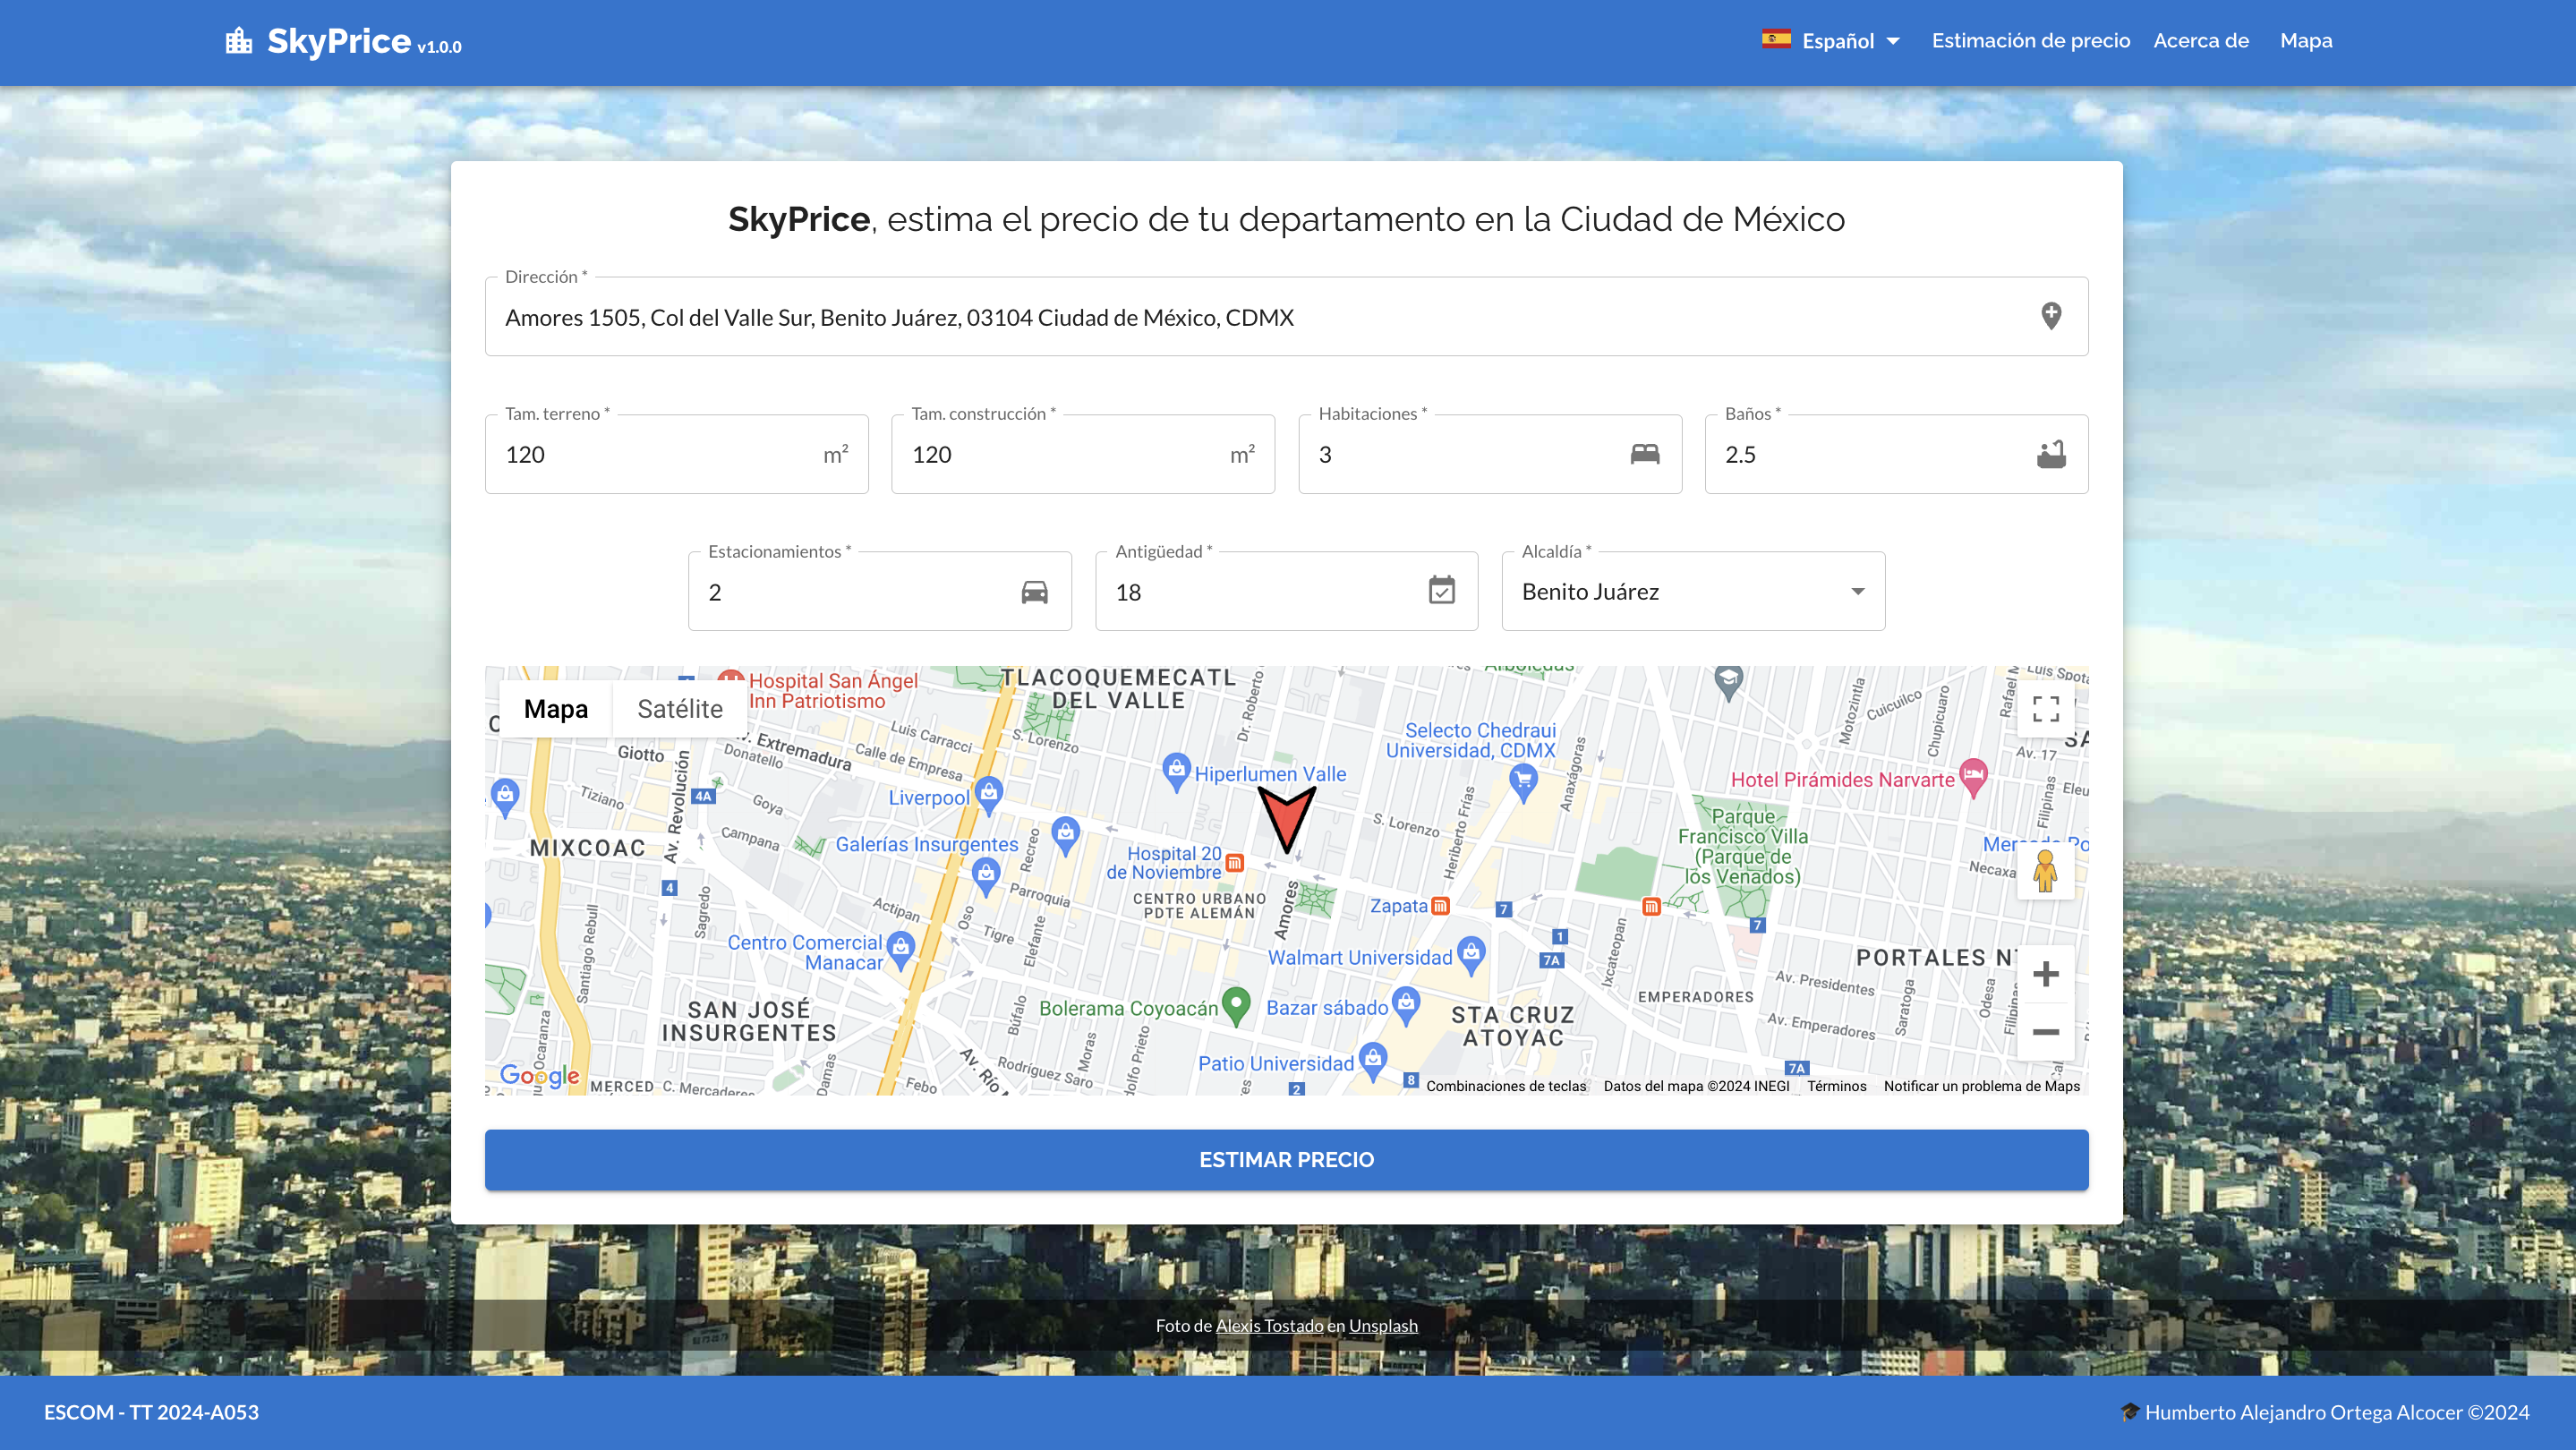
\includegraphics[width=1.0\textwidth]{imagenes/05-implementacion/interfaz-grafica/geocodificacion.png}
    \caption{Formulario con datos de una propiedad y mapa resultante de la geocodificación.}
    \label{fig:geocodificacion}
\end{figure}

\subsubsection{Resultados de la predicción}
Los resultados de la predicción se muestran en una sección debajo del formulario
de estimación de precio, donde los usuarios pueden ver las predicciones de los
modelos de Random Forest, Máquinas de Soporte Vectorial y Redes Neuronales. En la
figura \ref{fig:resultados-prediccion} se muestra la sección de resultados de la
predicción de la interfaz gráfica.

\begin{figure}[H]
    \centering
    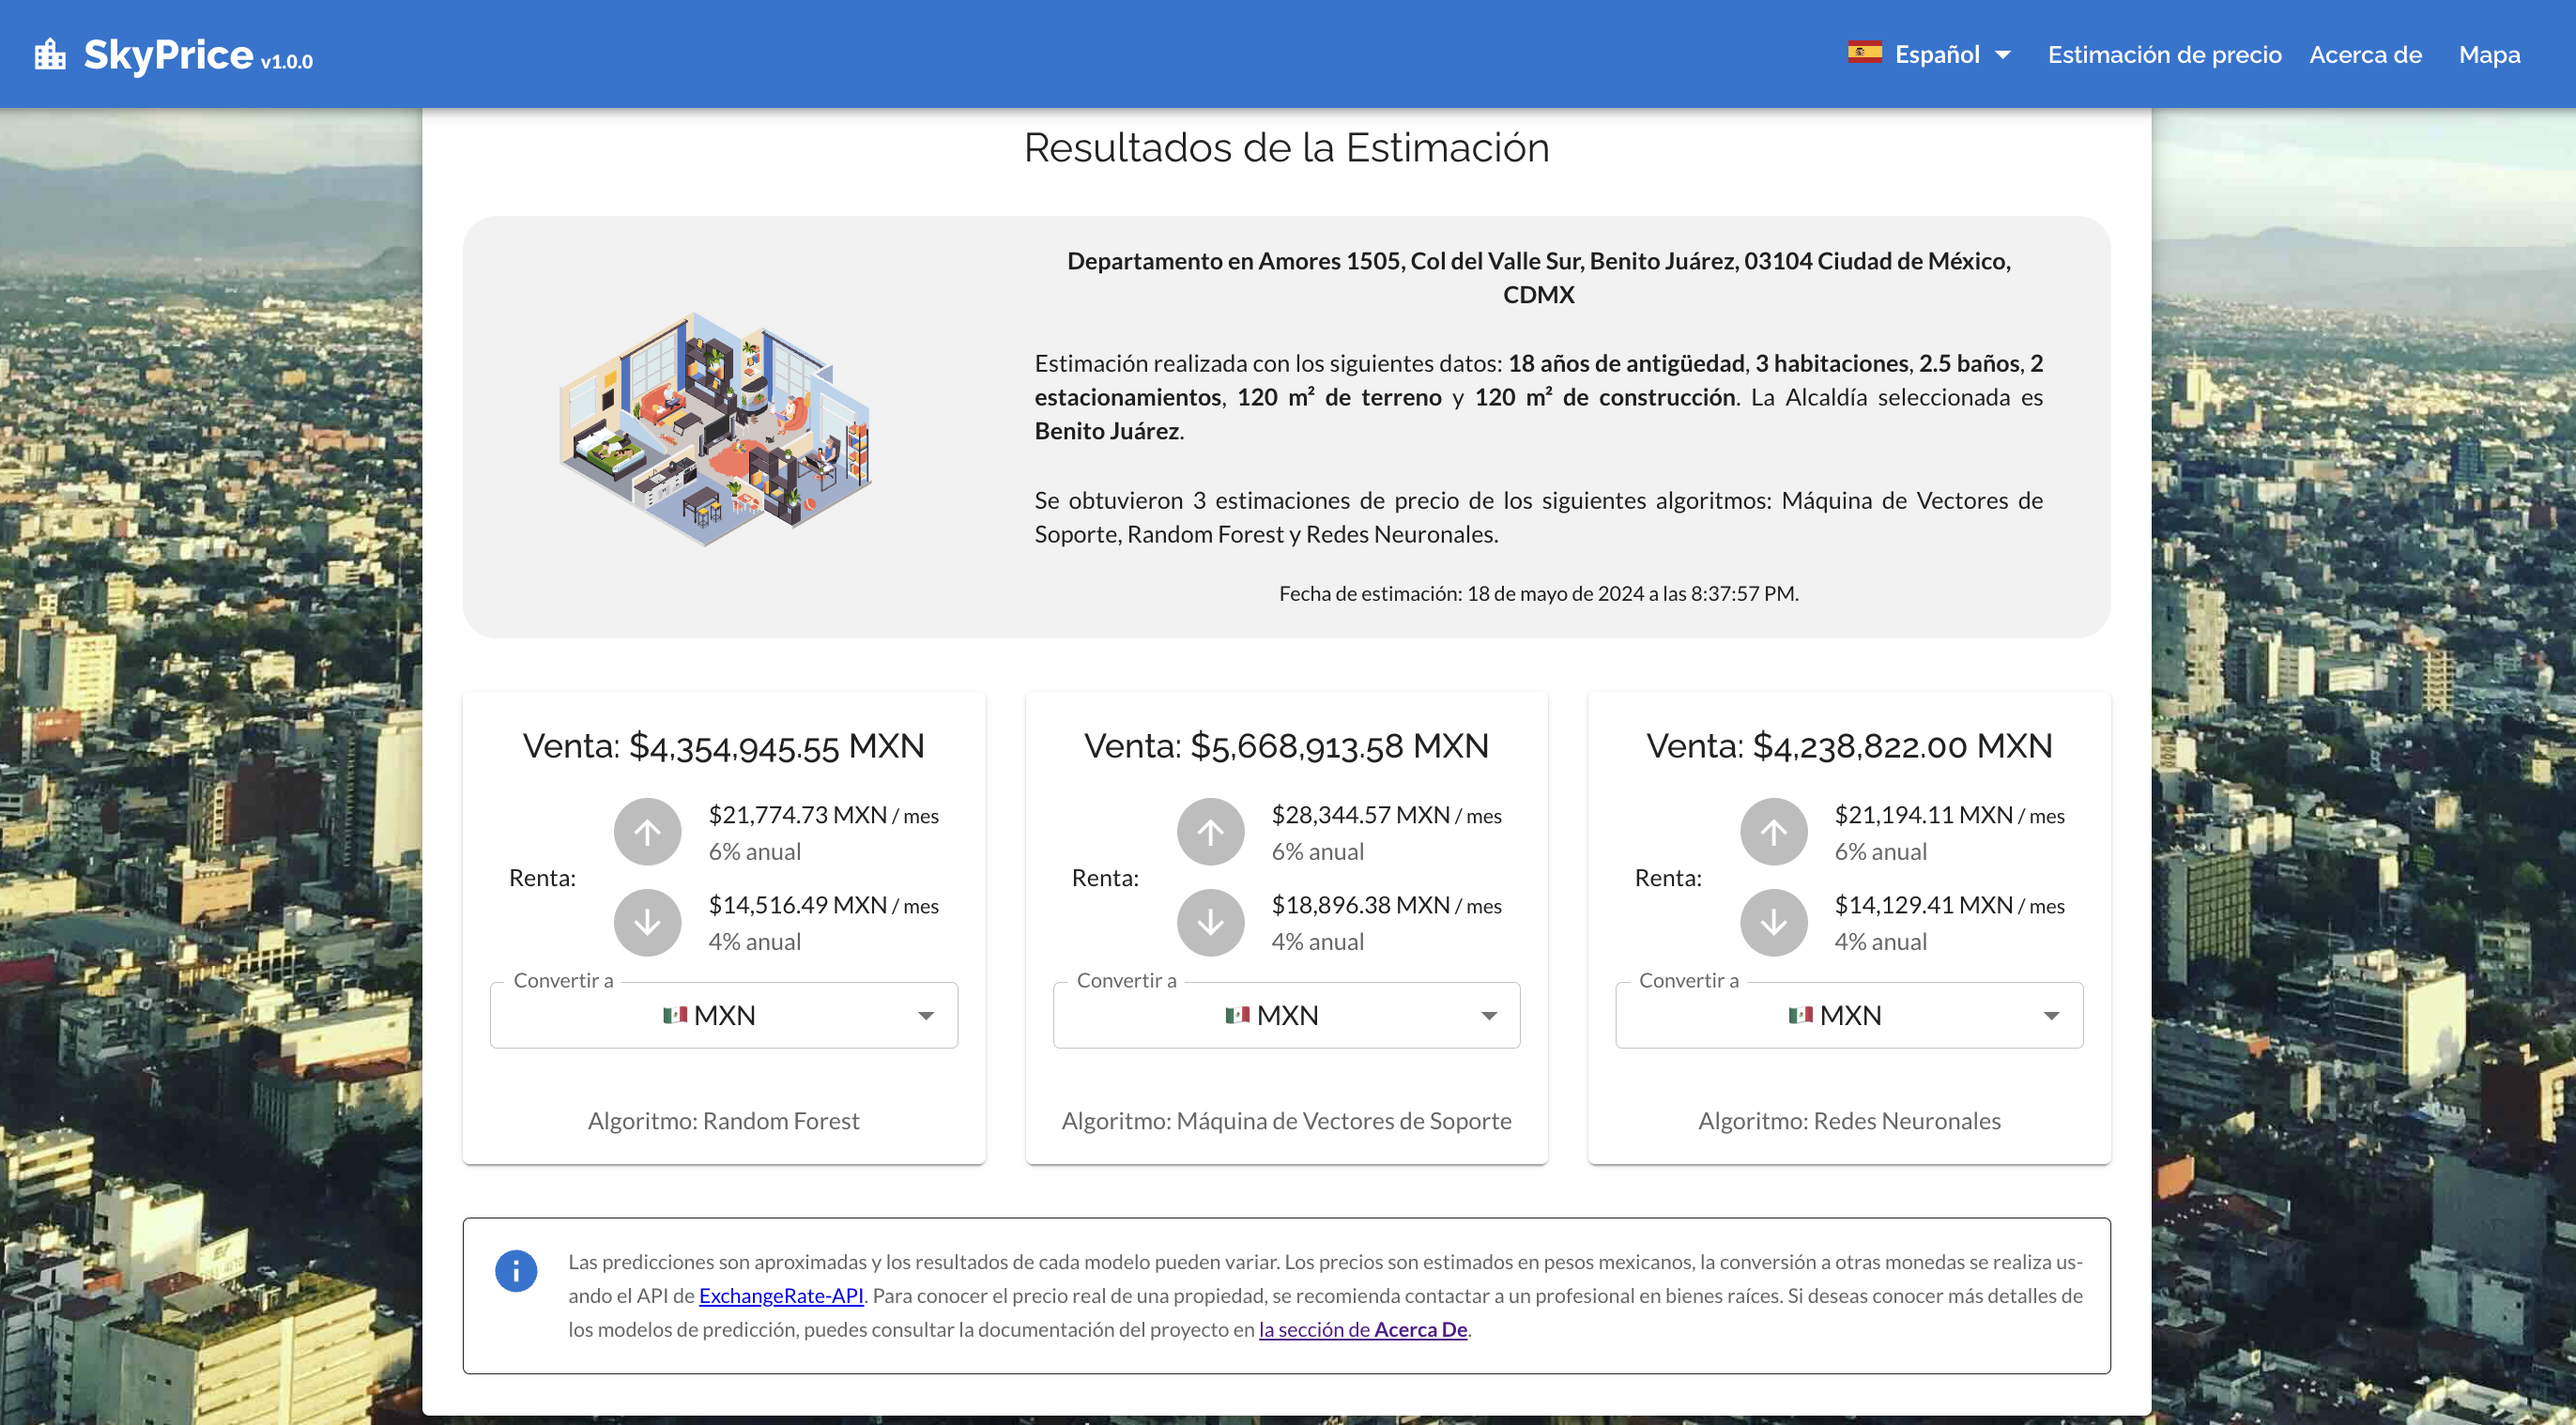
\includegraphics[width=1.0\textwidth]{imagenes/05-implementacion/interfaz-grafica/resultado-prediccion.png}
    \caption{Sección de resultados de la predicción de la interfaz gráfica.}
    \label{fig:resultados-prediccion}
\end{figure}

Como se puede apreciar en la figura \ref{fig:resultados-prediccion}, los resultados
de la predicción incluyen una estimación de precio de venta por modelo, así como
estimaciones de precios de renta mensual calculada al 4\% - 6\% del precio de venta.

Adicionalmente, cada estimación de precios incluye un convertidor de moneda que
permite al usuario ver el precio en dólares estadounidenses (USD), euros (EUR),
dólares canadienses (CAD) entre otros más. En la figura \ref{fig:conversor-moneda}
se muestran las opciones de conversión de moneda disponibles.

\begin{figure}[H]
    \centering
    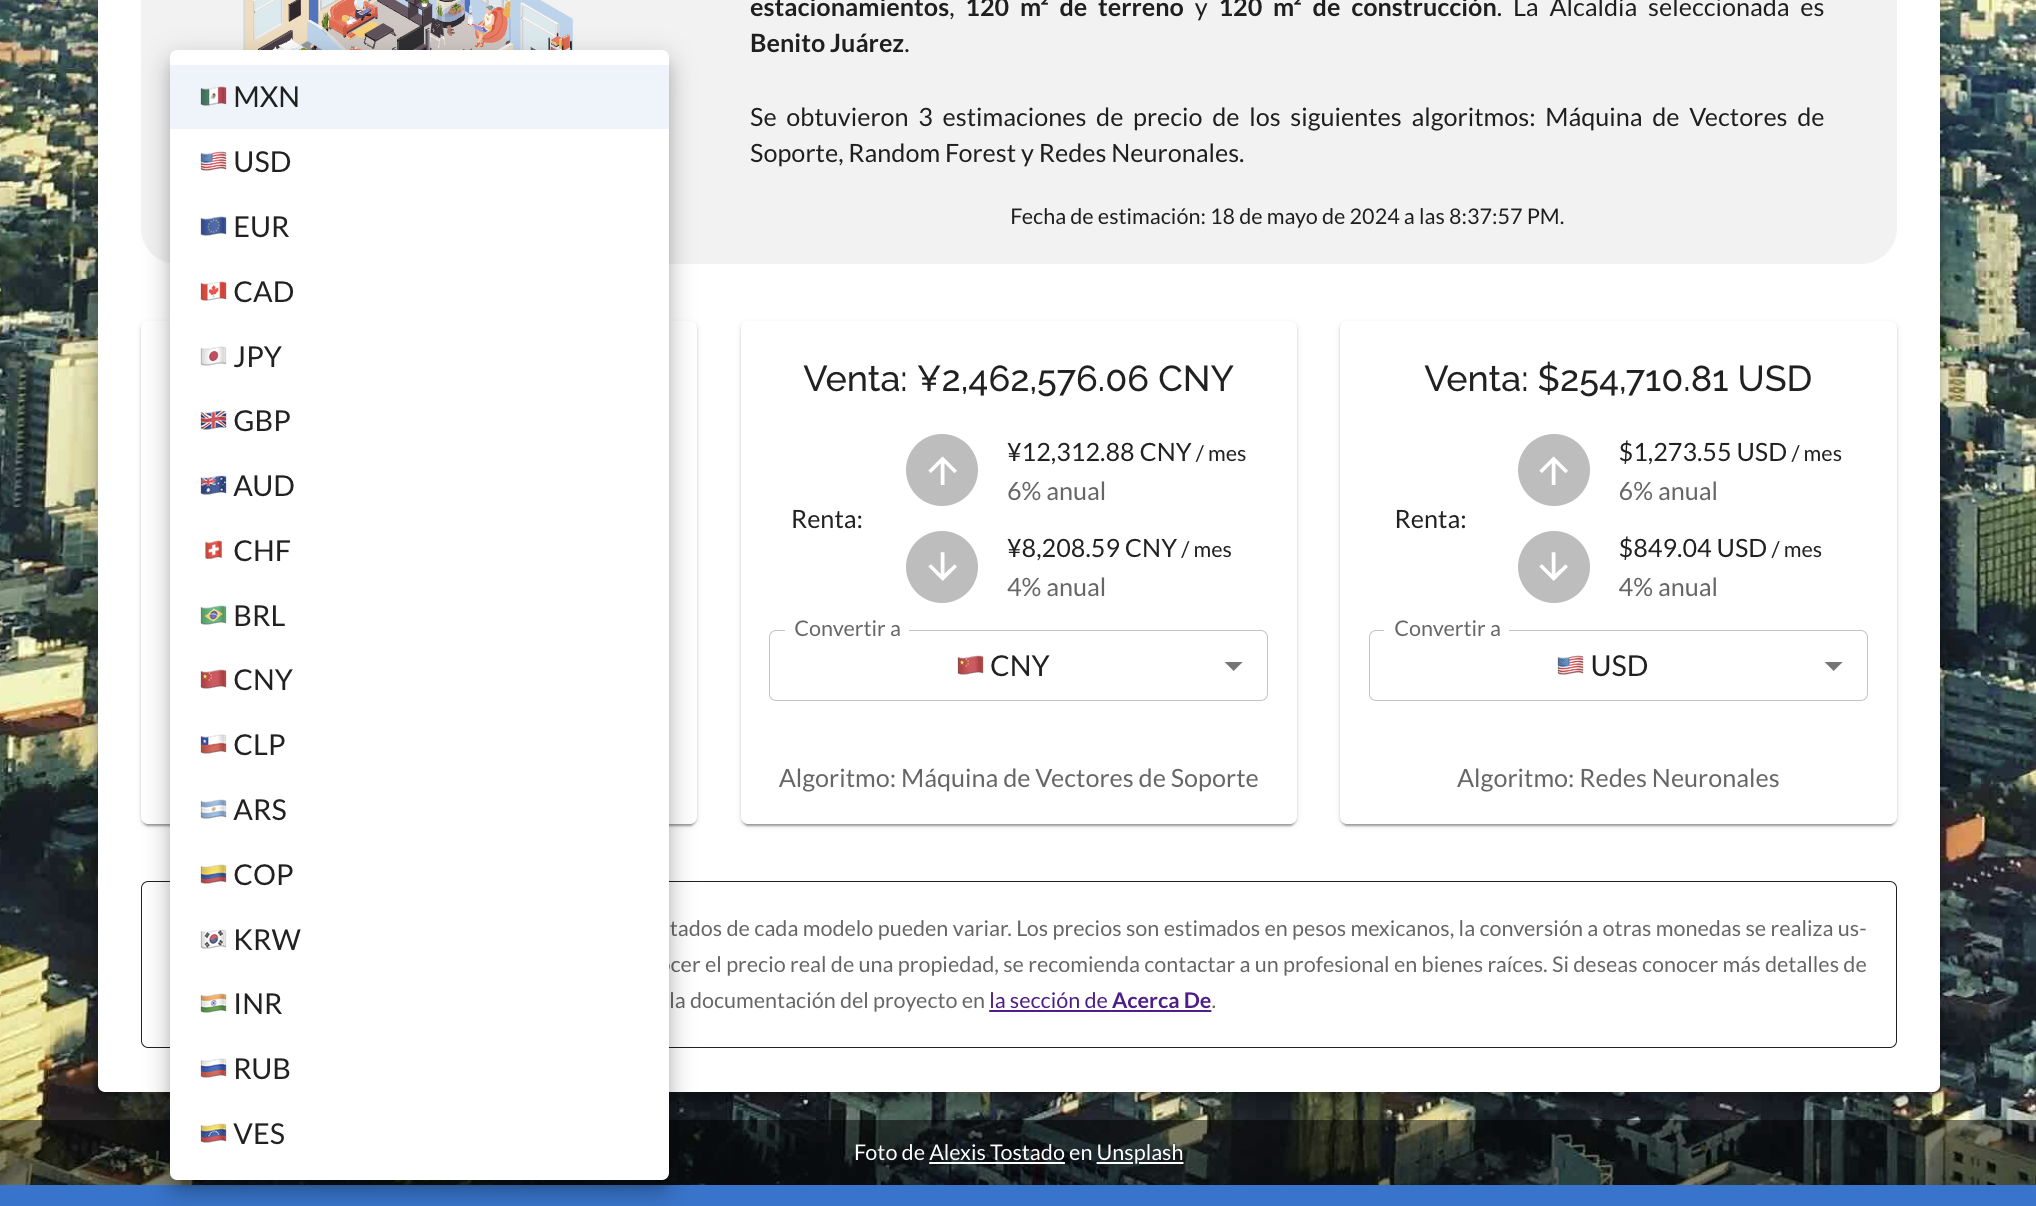
\includegraphics[width=1.0\textwidth]{imagenes/05-implementacion/interfaz-grafica/conversor-moneda.png}
    \caption{Opciones de conversión de moneda en la interfaz gráfica.}
    \label{fig:conversor-moneda}
\end{figure}

\subsection{Acerca de}
La página de Acerca de incluye información sobre el proyecto, los modelos de
aprendizaje automático utilizados, información sobre los datos y enlaces a la
documentación de la API.

\subsubsection{Proyecto en general}
La primer sección de la página de Acerca de incluye información general sobre el
proyecto, incluyendo el título, la descripción, el autor y la fecha de creación. En
la figura \ref{fig:acerca-de-proyecto} se muestra la sección de información general
de la página de Acerca de.

\begin{figure}[H]
    \centering
    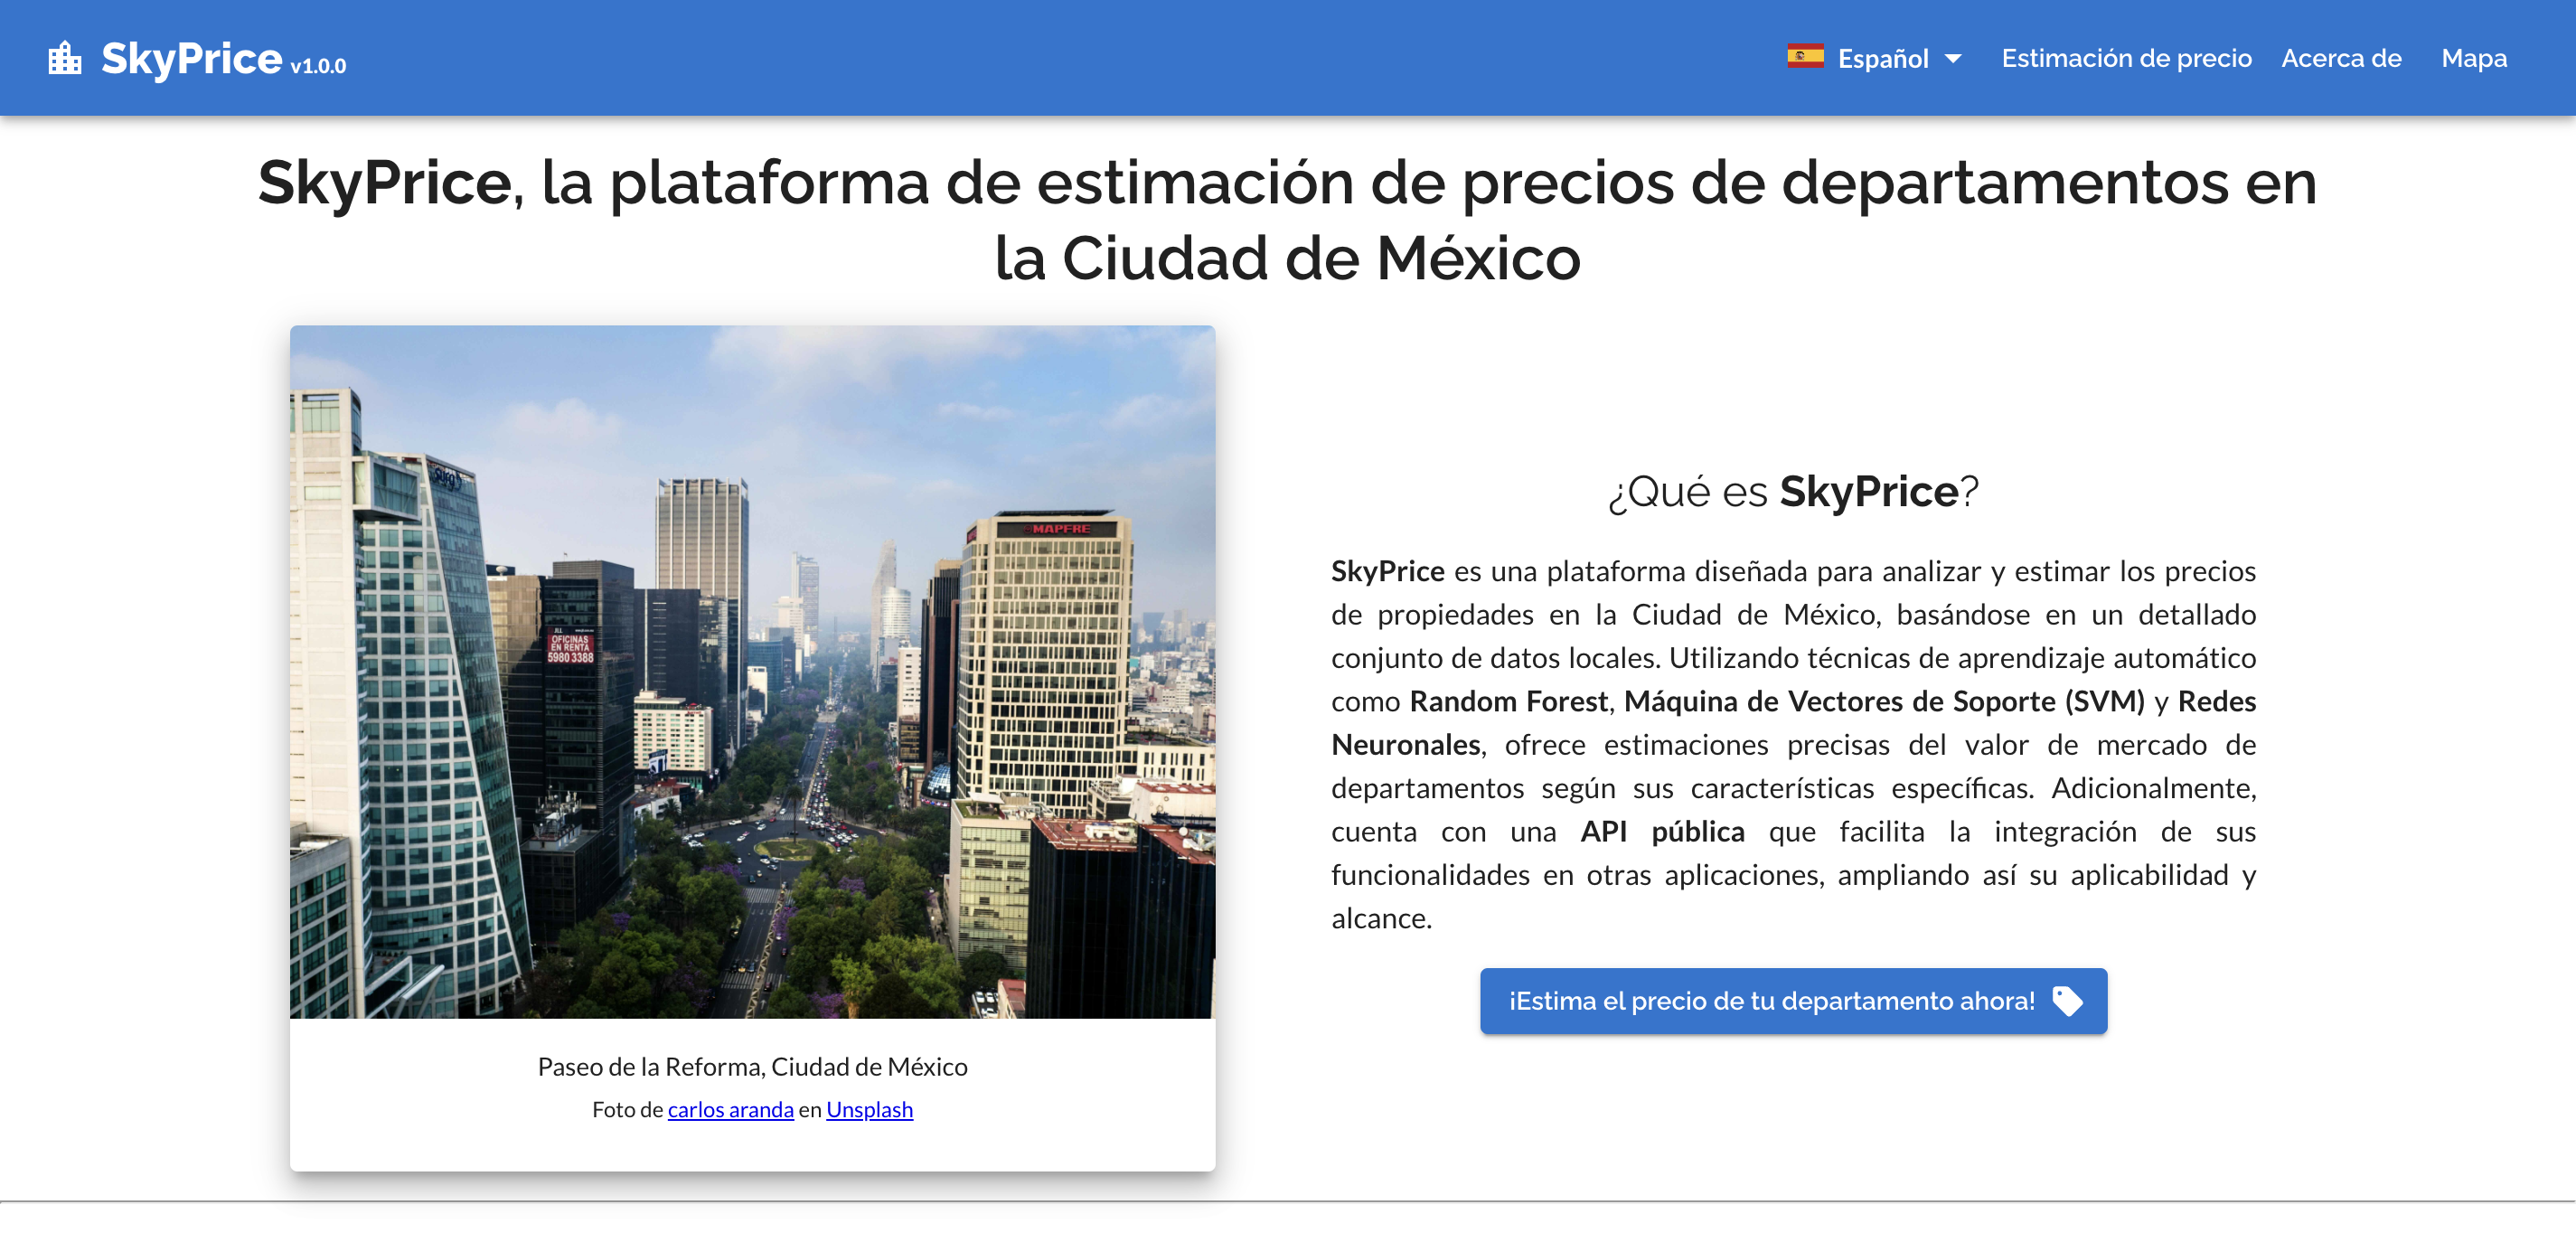
\includegraphics[width=1.0\textwidth]{imagenes/05-implementacion/interfaz-grafica/acerca-de-proyecto.png}
    \caption{Sección de información general de la página de Acerca de.}
    \label{fig:acerca-de-proyecto}
\end{figure}

\subsubsection{Datos}
La segunda sección de la página de Acerca de incluye información sobre los datos
utilizados en el proyecto, incluyendo el tamaño del conjunto de datos, la cantidad
de características y la división en conjuntos de entrenamiento y prueba. En la figura
\ref{fig:acerca-de-datos} se muestra la sección de información sobre los datos de la
página de Acerca de.

\begin{figure}[H]
    \centering
    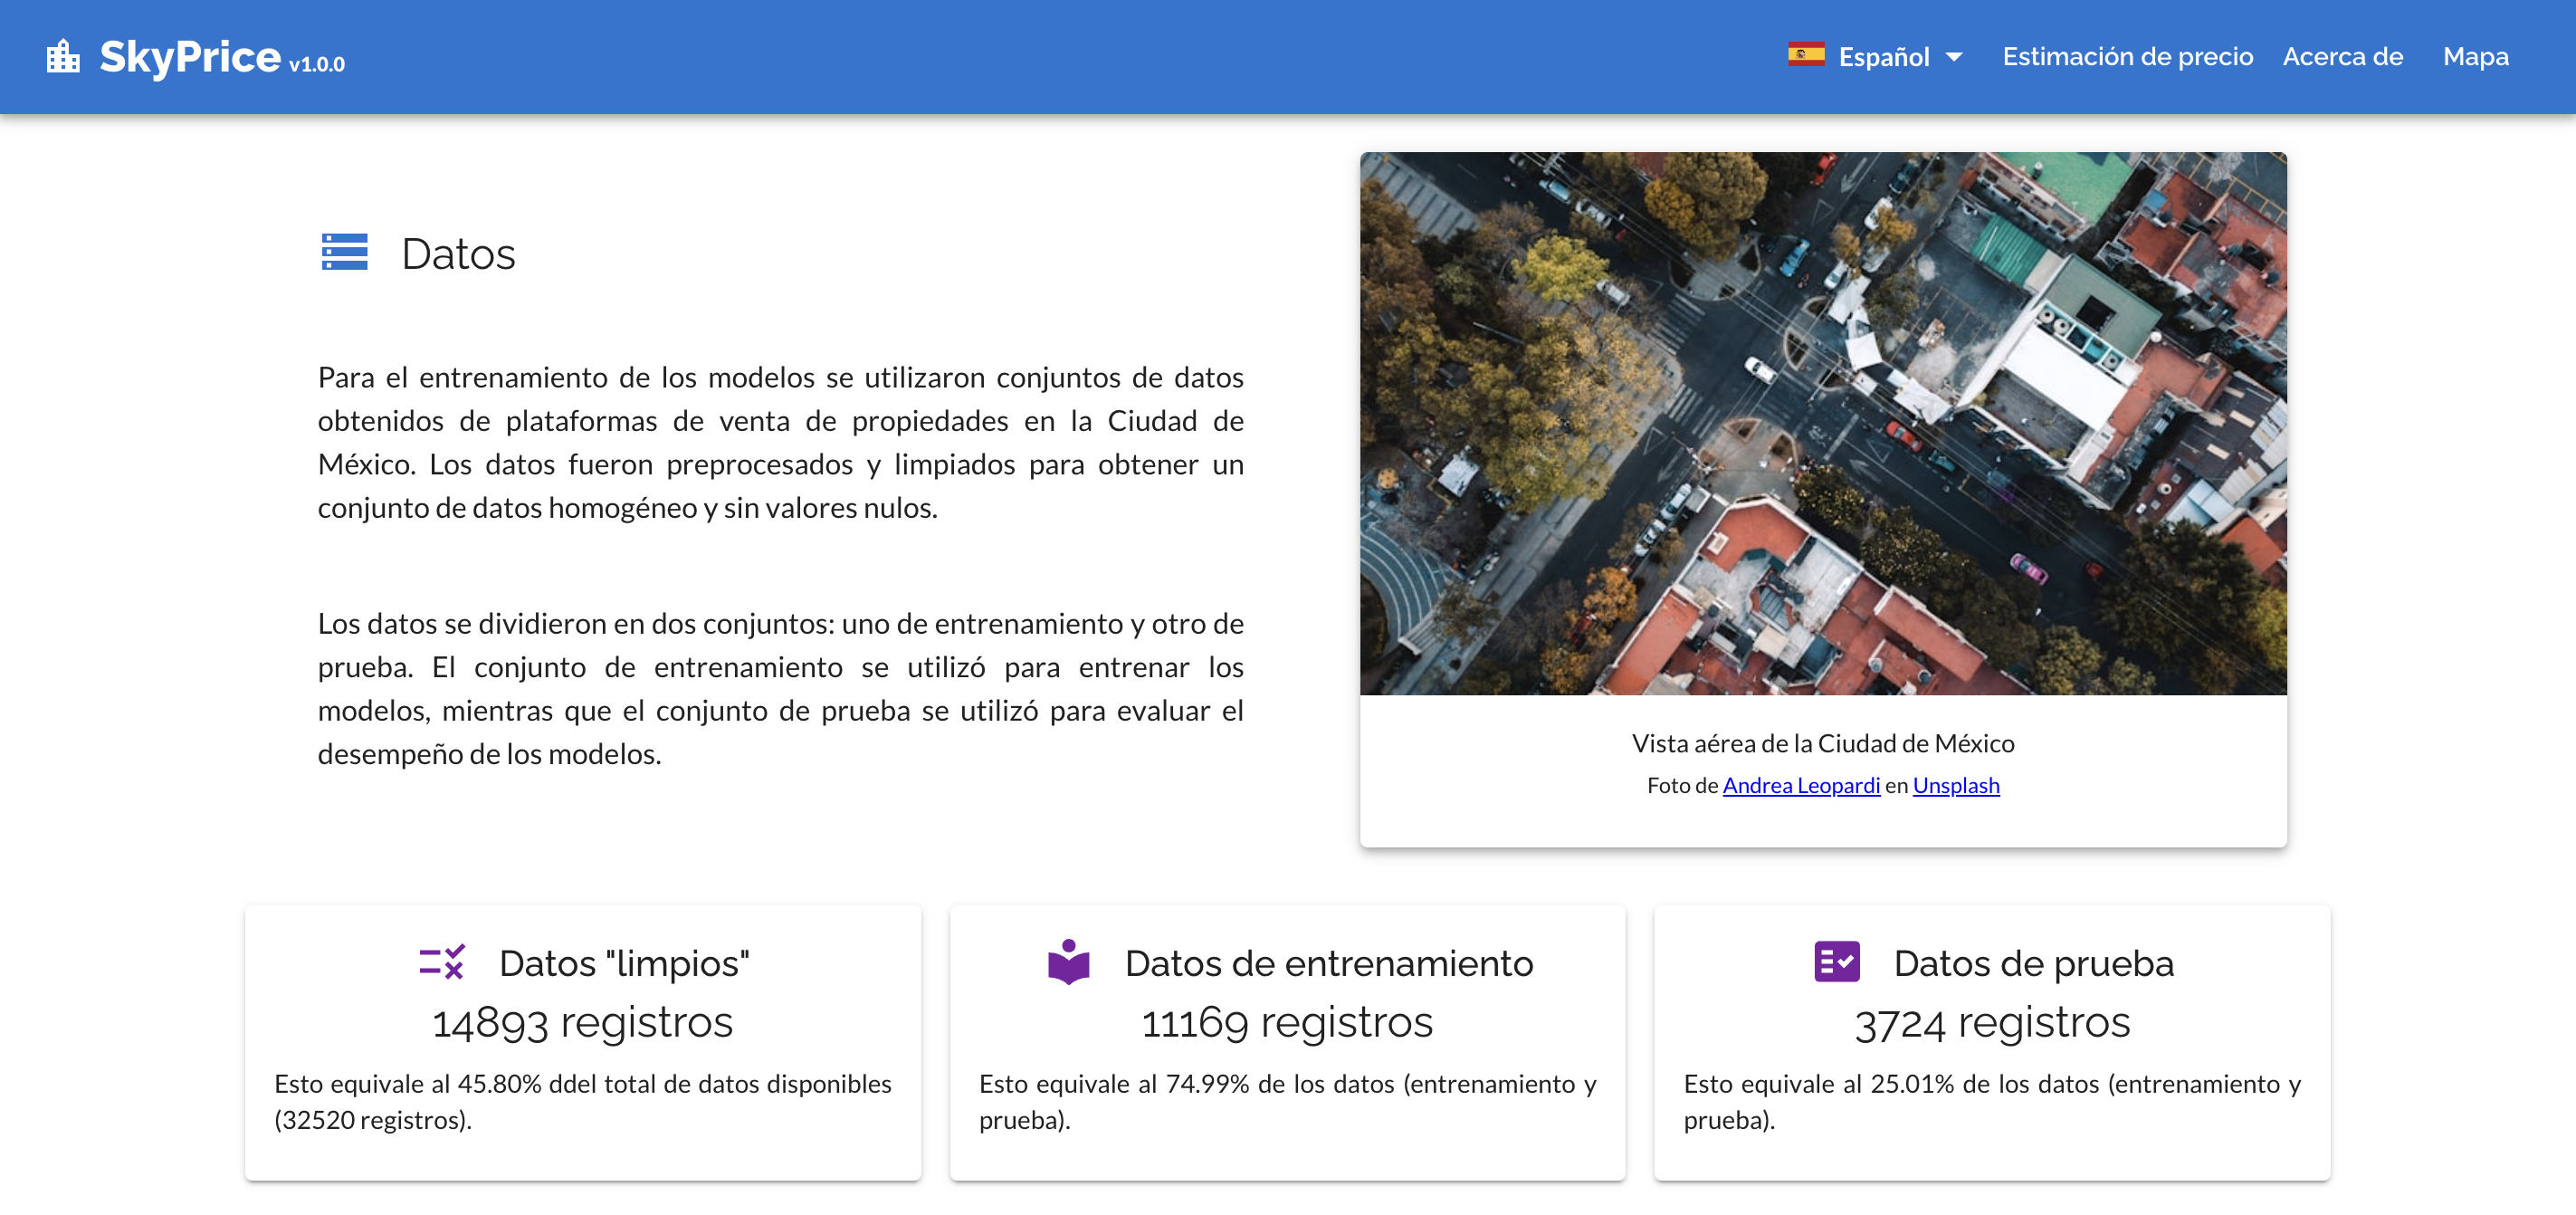
\includegraphics[width=1.0\textwidth]{imagenes/05-implementacion/interfaz-grafica/acerca-de-datos.png}
    \caption{Sección de información sobre los datos de la página de Acerca de.}
    \label{fig:acerca-de-datos}
\end{figure}

También se incluye una pequeña sección sobre el mapa interactivo, que permite a los
usuarios visualizar los datos en cuestión geoespacialmente usando Kepler.gl. En la
figura \ref{fig:acerca-de-mapa} se muestra la sección de información sobre el mapa
interactivo de la página de Acerca de.

\begin{figure}[H]
    \centering
    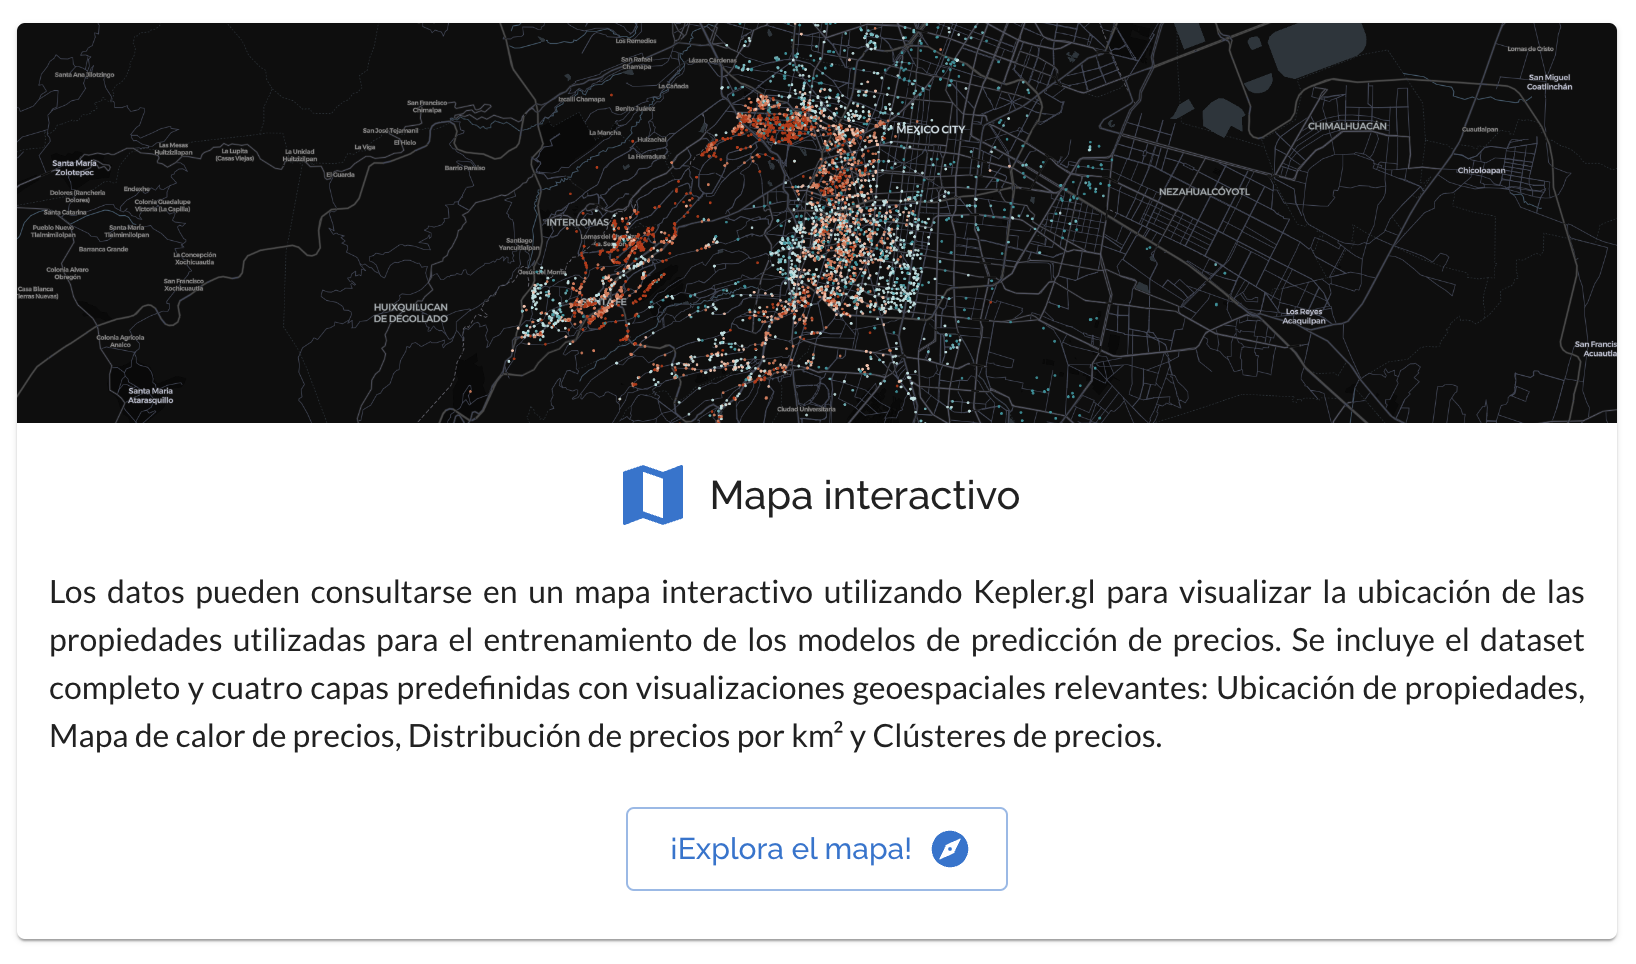
\includegraphics[width=1.0\textwidth]{imagenes/05-implementacion/interfaz-grafica/acerca-de-mapa.png}
    \caption{Sección de información sobre el mapa interactivo de la página de Acerca de.}
    \label{fig:acerca-de-mapa}
\end{figure}

\subsubsection{Modelos de aprendizaje automático}
La siguiente sección de la página de Acerca de incluye información sobre los modelos
de aprendizaje automático utilizados en el proyecto, incluyendo Random Forest, Máquinas
de Soporte Vectorial y Redes Neuronales. En la figura \ref{fig:acerca-de-modelos} se
muestra la sección de información sobre los modelos de aprendizaje automático, que
incluye métricas de evaluación, hiperparámetros y características importantes.

\begin{figure}[H]
    \centering
    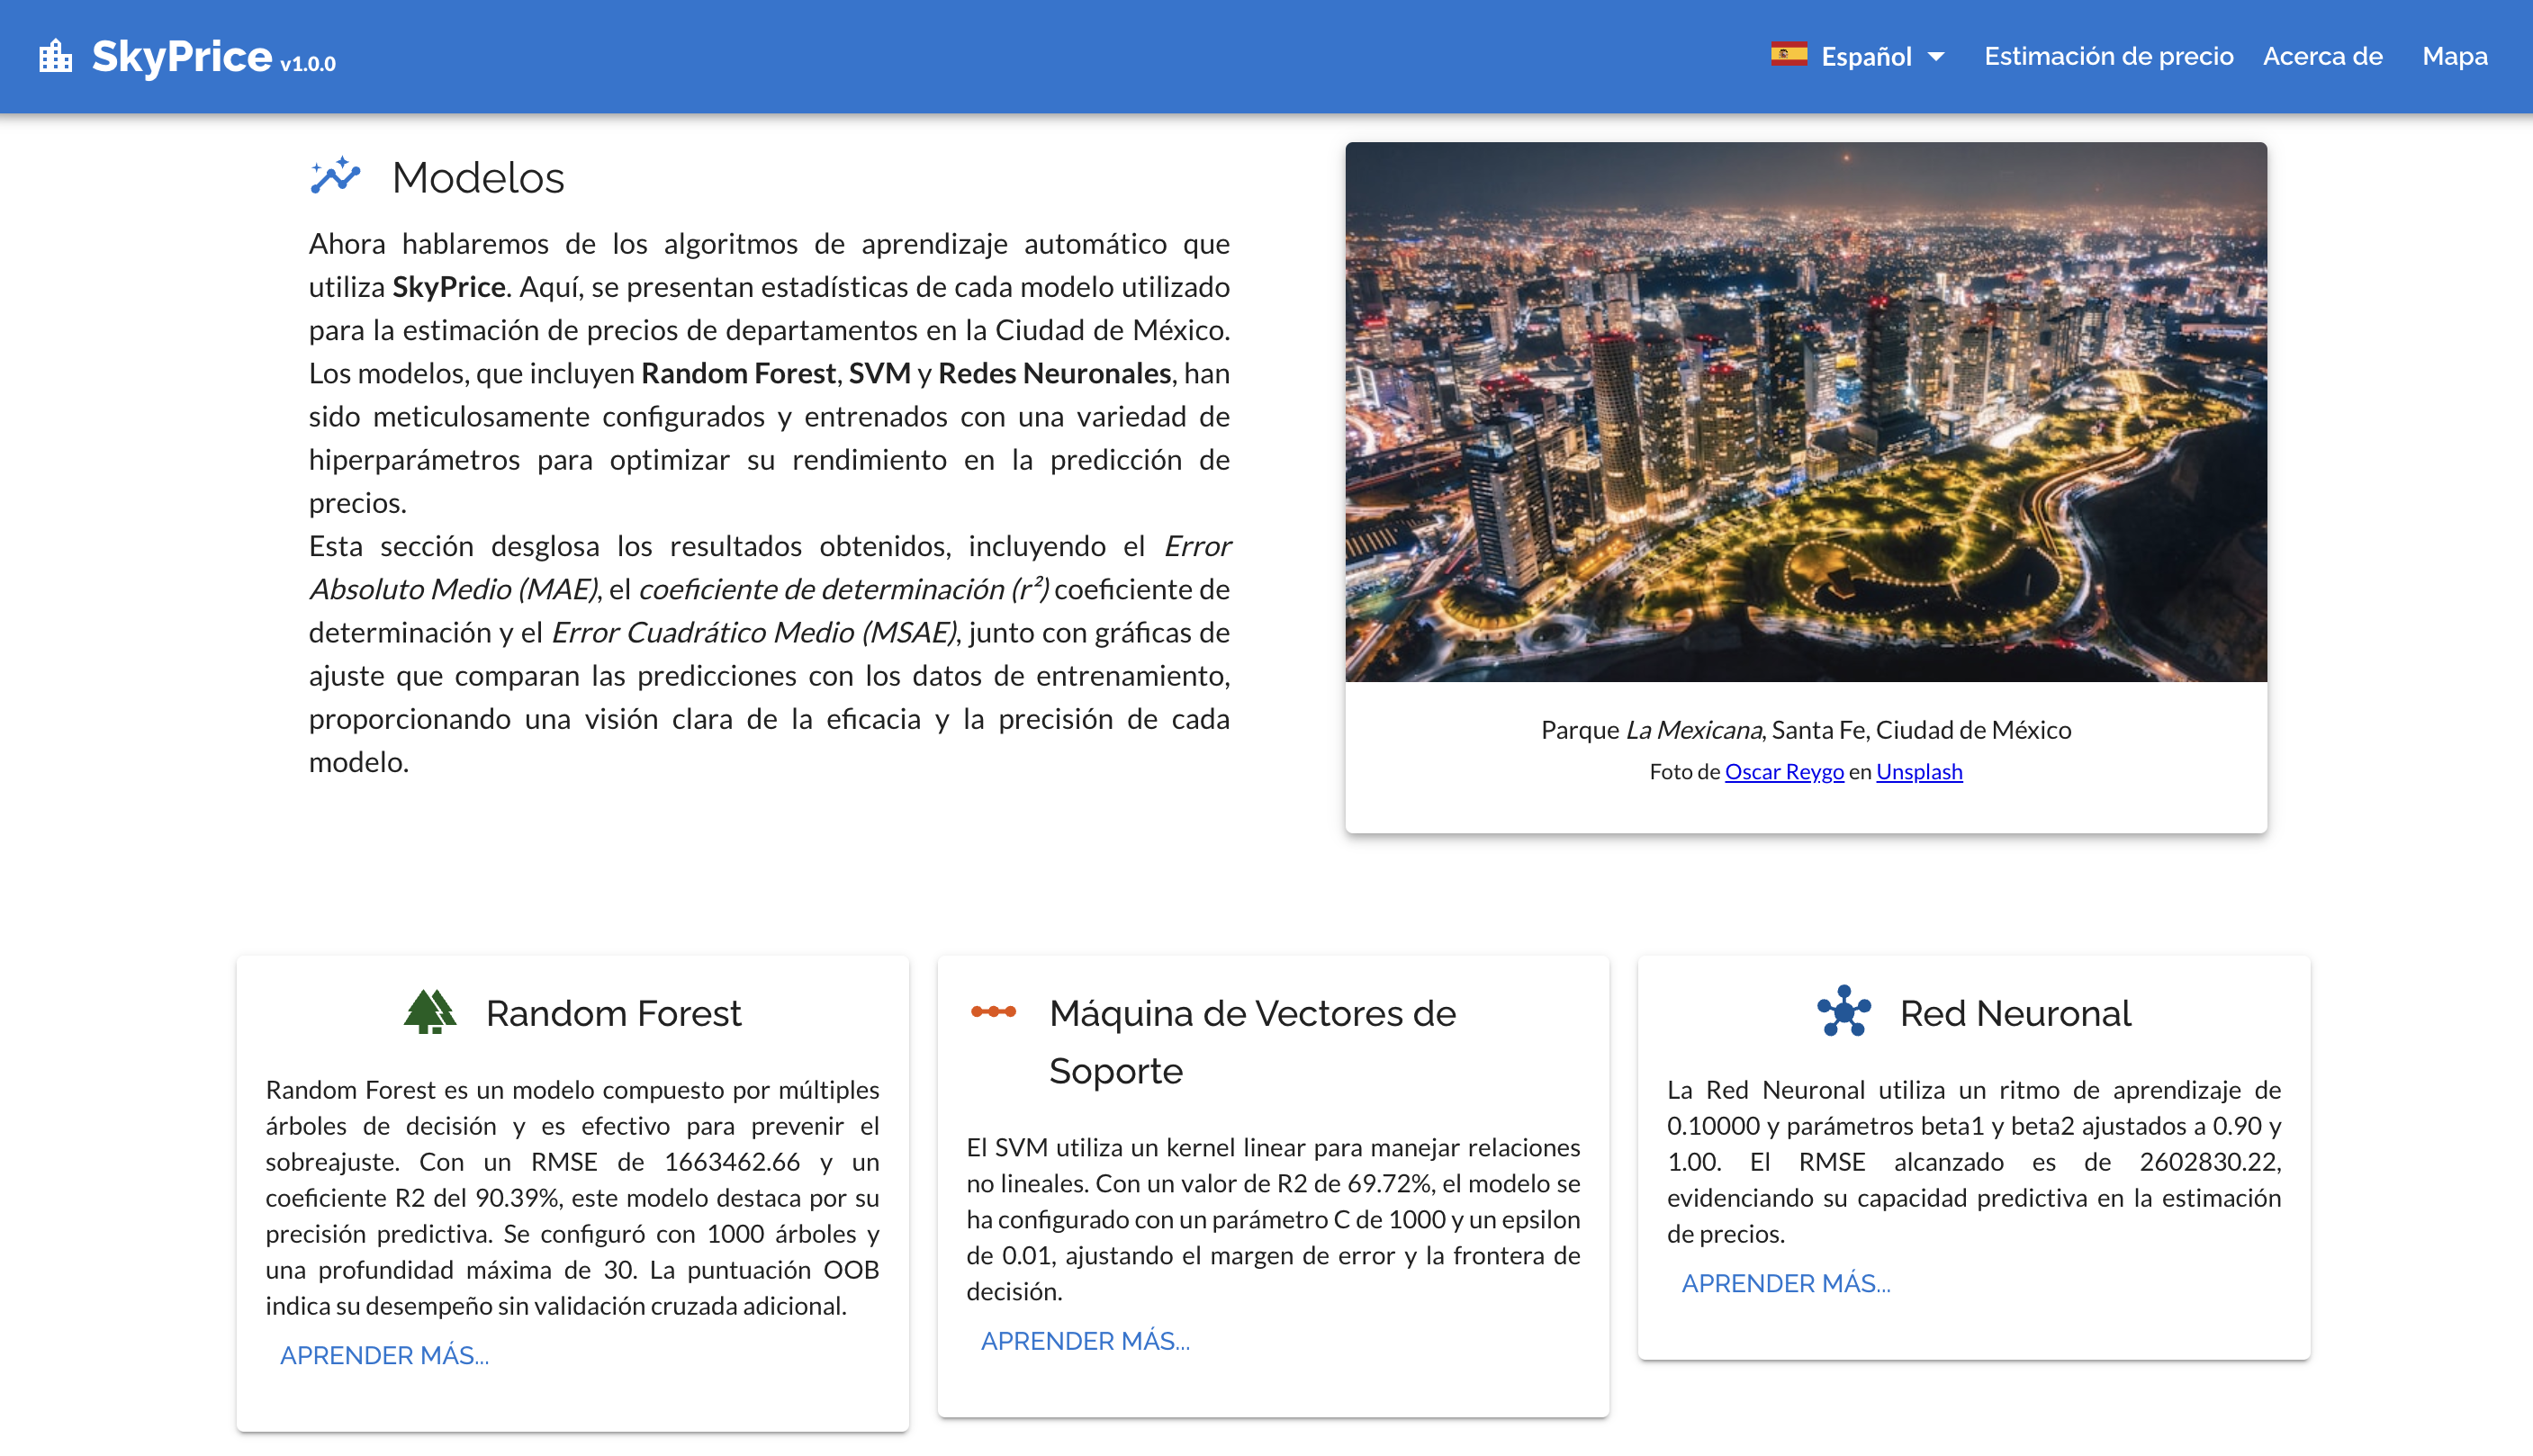
\includegraphics[width=1.0\textwidth]{imagenes/05-implementacion/interfaz-grafica/acerca-de-modelos.png}
    \caption{Sección de información sobre los modelos de aprendizaje automático de la página de Acerca de.}
    \label{fig:acerca-de-modelos}
\end{figure}

Además, se incluyen dos gráficas que muestran las predicciones de los modelos de
Random Forest, Máquinas de Soporte Vectorial y Redes Neuronales en comparación con
los valores reales y una comparativa de las métricas de evaluación de los modelos.
En la figura \ref{fig:acerca-de-graficas} se muestra la sección de gráficas de la
página de Acerca de.

\begin{figure}[H]
    \centering
    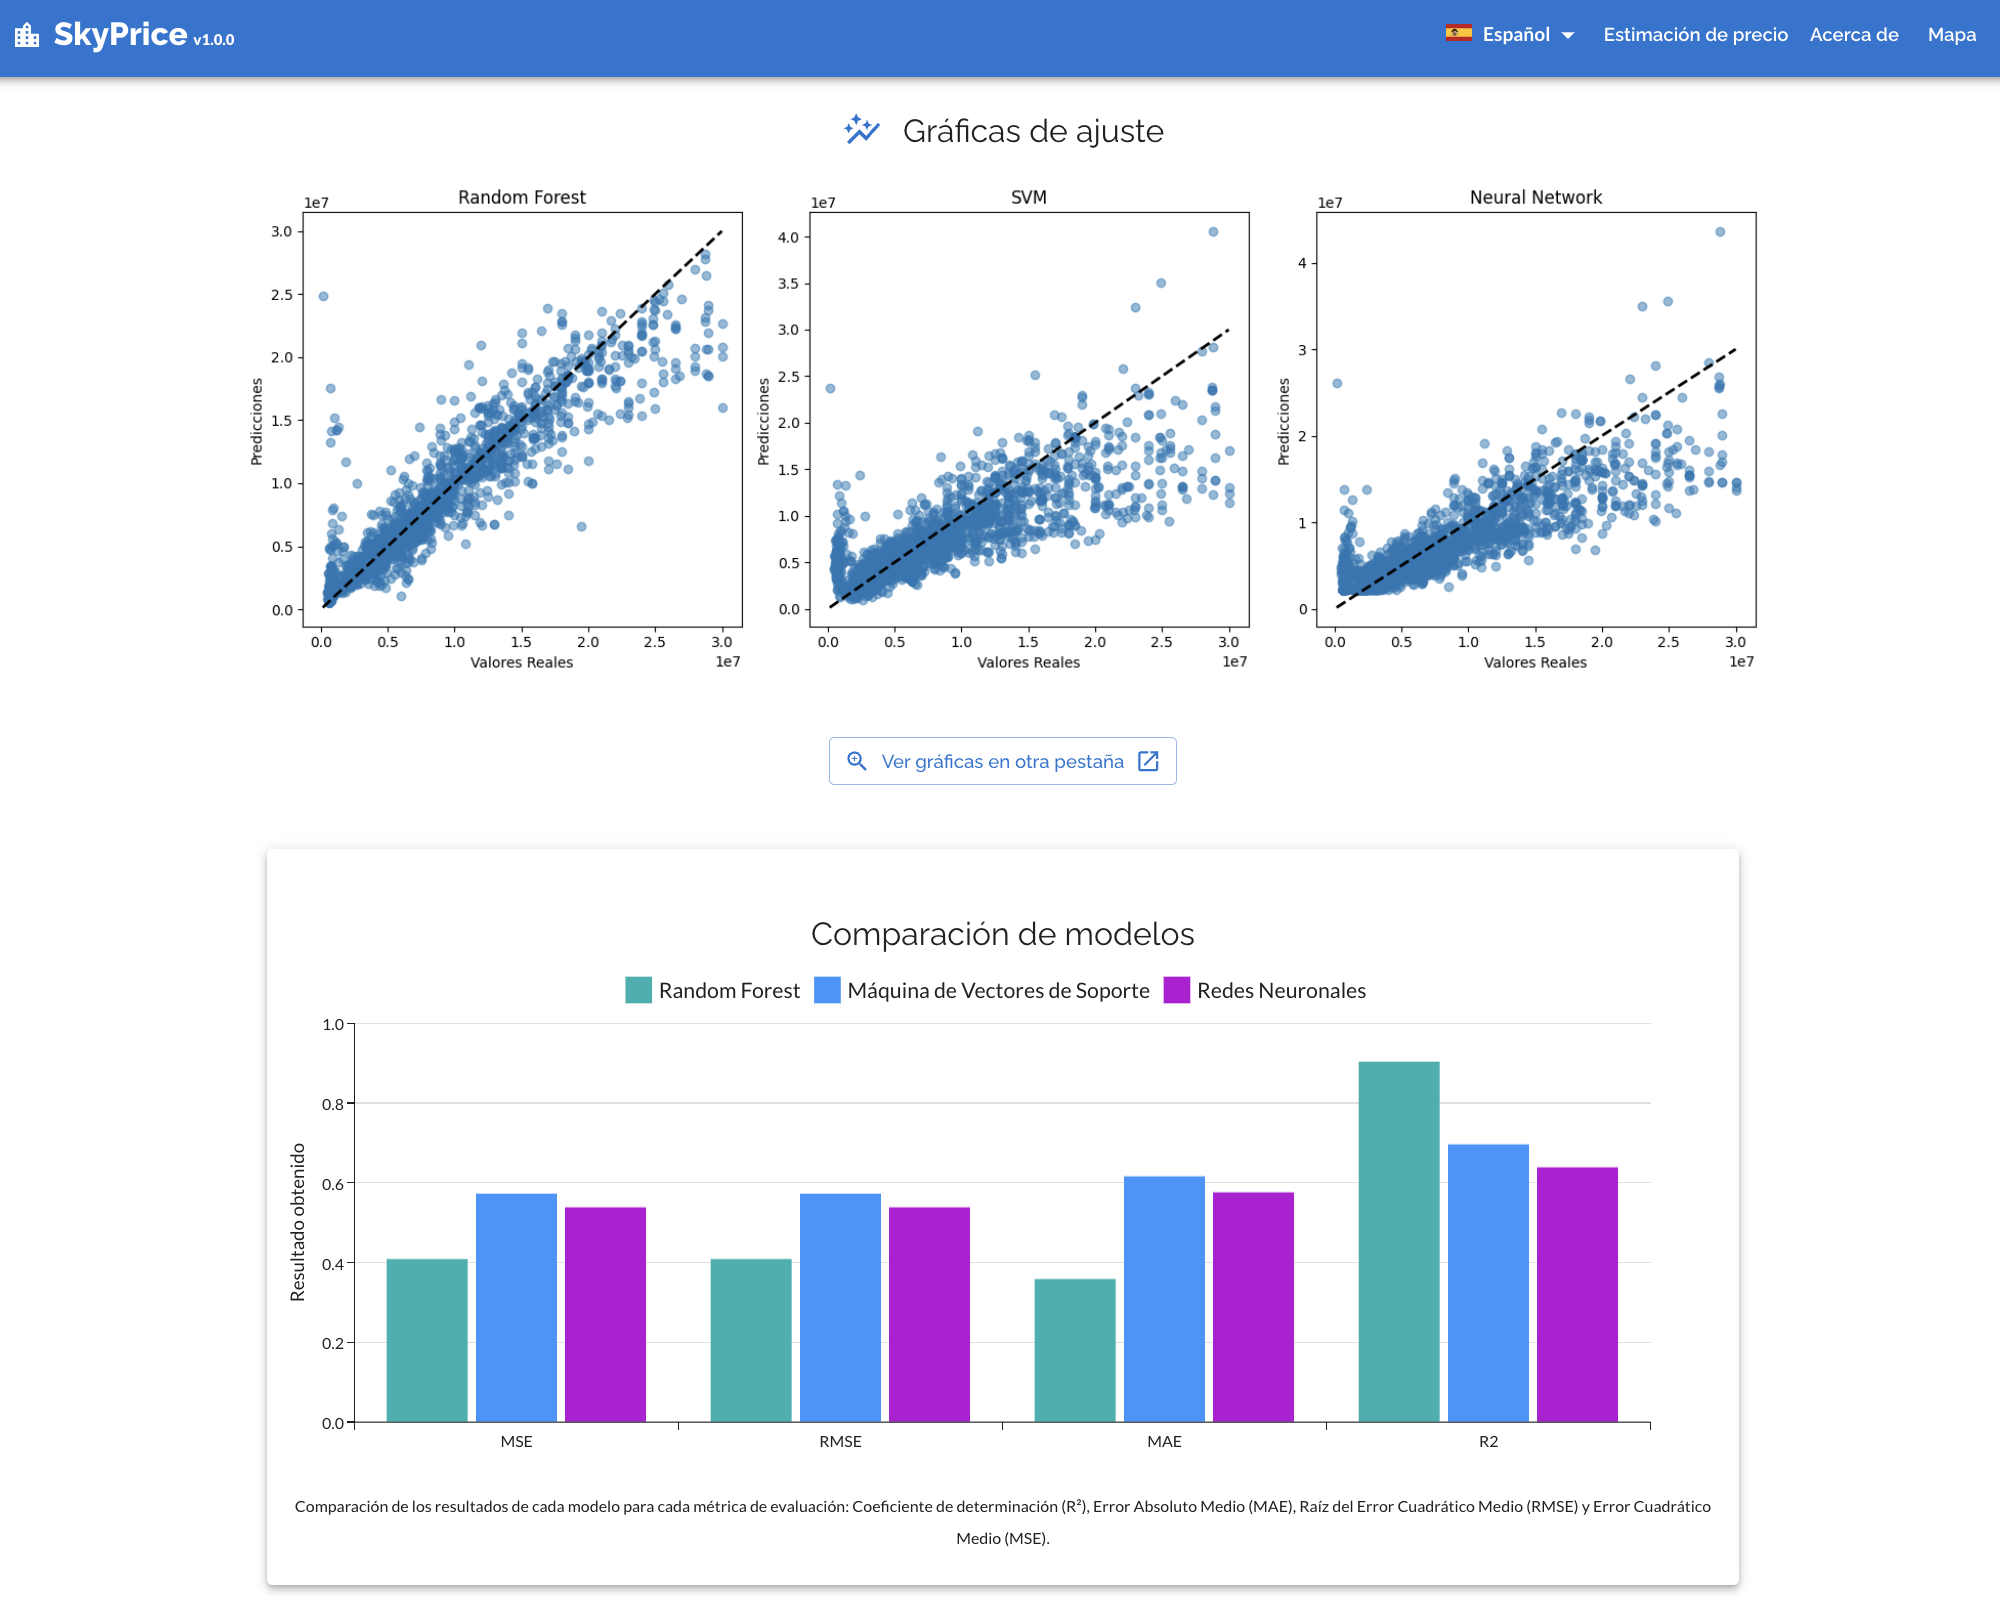
\includegraphics[width=1.0\textwidth]{imagenes/05-implementacion/interfaz-grafica/acerca-de-modelos-graficas.png}
    \caption{Sección de gráficas de la página de Acerca de.}
    \label{fig:acerca-de-graficas}
\end{figure}

\subsubsection{Documentación de la API y créditos}
La penúltima sección de la página de Acerca de incluye enlaces a la documentación
de la API en formato OpenAPI (Swagger) y ReDoc, lo que permite a los usuarios explorar
los endpoints, los modelos y los parámetros de la API de manera interactiva y visual.
Además, se incluyen los créditos del proyecto.
En la figura \ref{fig:acerca-de-documentacion} se muestra la sección de documentación
de la página de Acerca de.

\begin{figure}[H]
    \centering
    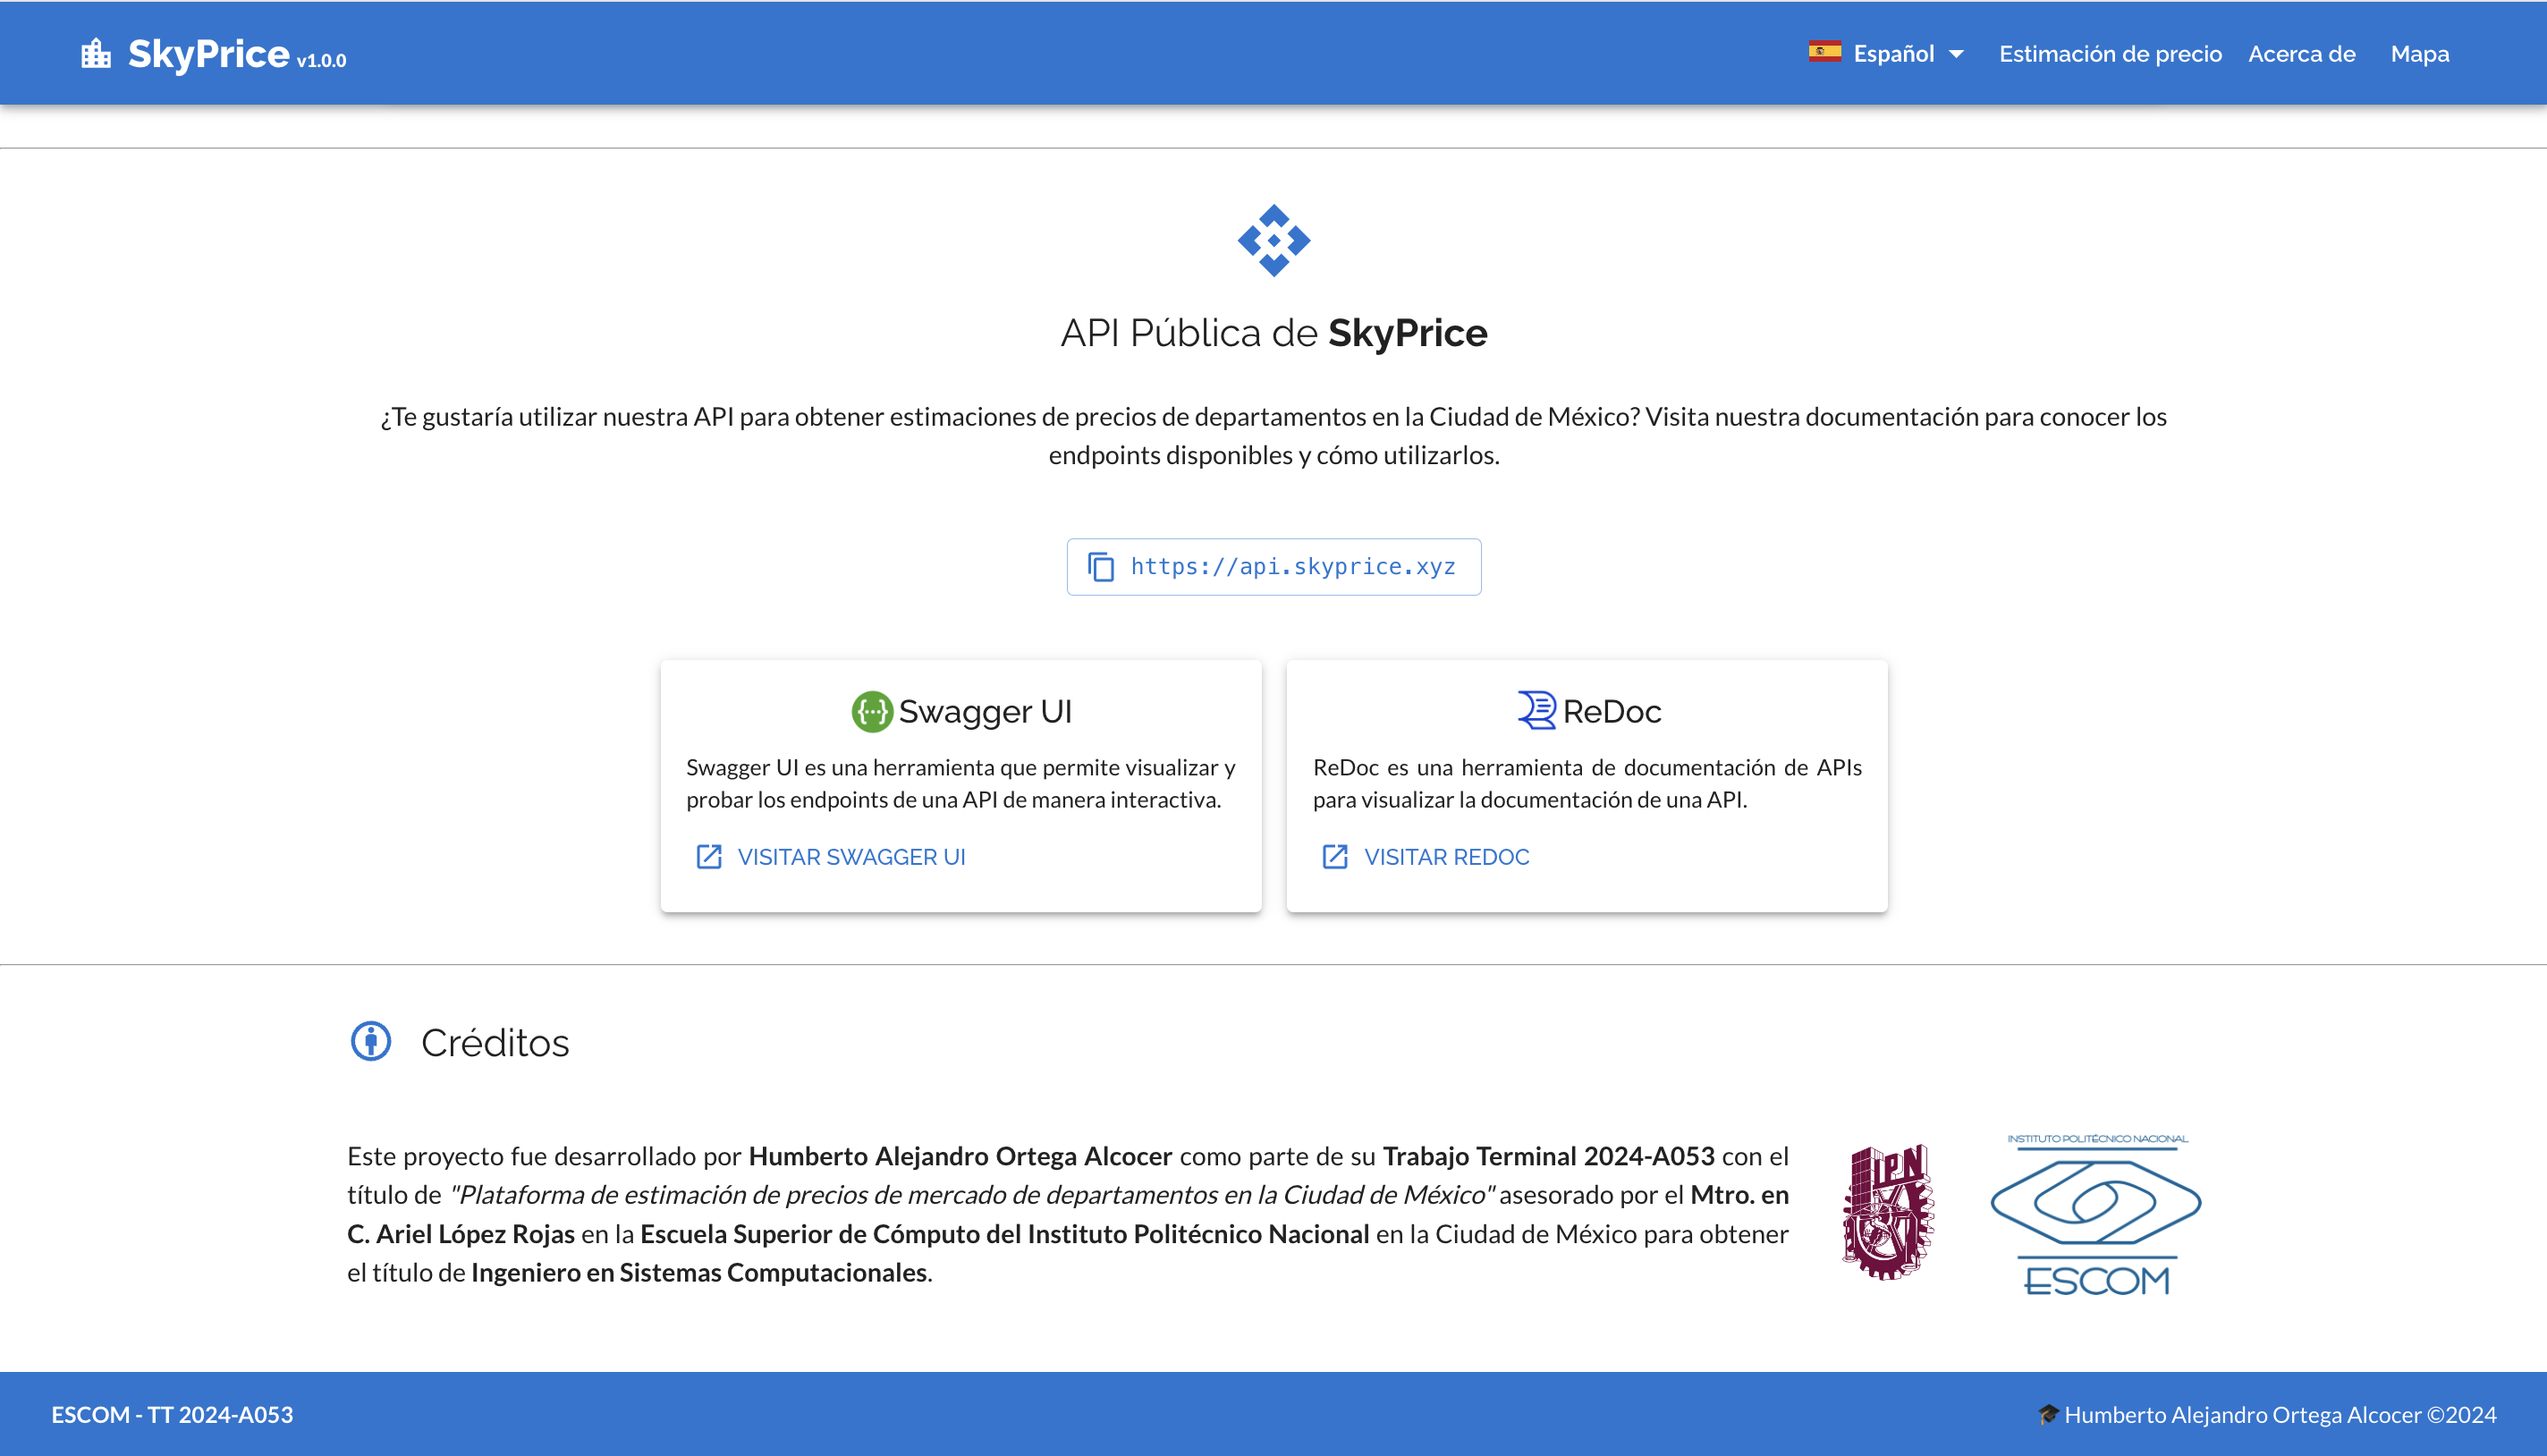
\includegraphics[width=1.0\textwidth]{imagenes/05-implementacion/interfaz-grafica/acerca-de-documentacion.png}
    \caption{Sección de documentación de la página de Acerca de.}
    \label{fig:acerca-de-documentacion}
\end{figure}

\subsection{Mapa interactivo}
La página de Mapa interactivo se desarrolló utilizando Kepler.gl, una biblioteca
de código abierto para la visualización de datos geoespaciales. La página permite
a los usuarios visualizar los datos de propiedades en la Ciudad de México empleados
en el proyecto, además de otras capas de datos relevantes.

Dado que los datos contenidos en las capas puede ser bastante extenso, se incluyó
una alerta que informa al usuario que la carga de los datos puede consumir
datos móviles, por lo que puede elegir si desea cargar el mapa dinámico o no,
en cuyo caso se mostrará una imagen estática del mapa. En la figura
\ref{fig:mapa-interactivo} se muestra la página de Mapa inicialmente con la alerta
de carga de datos.

\begin{figure}[H]
    \centering
    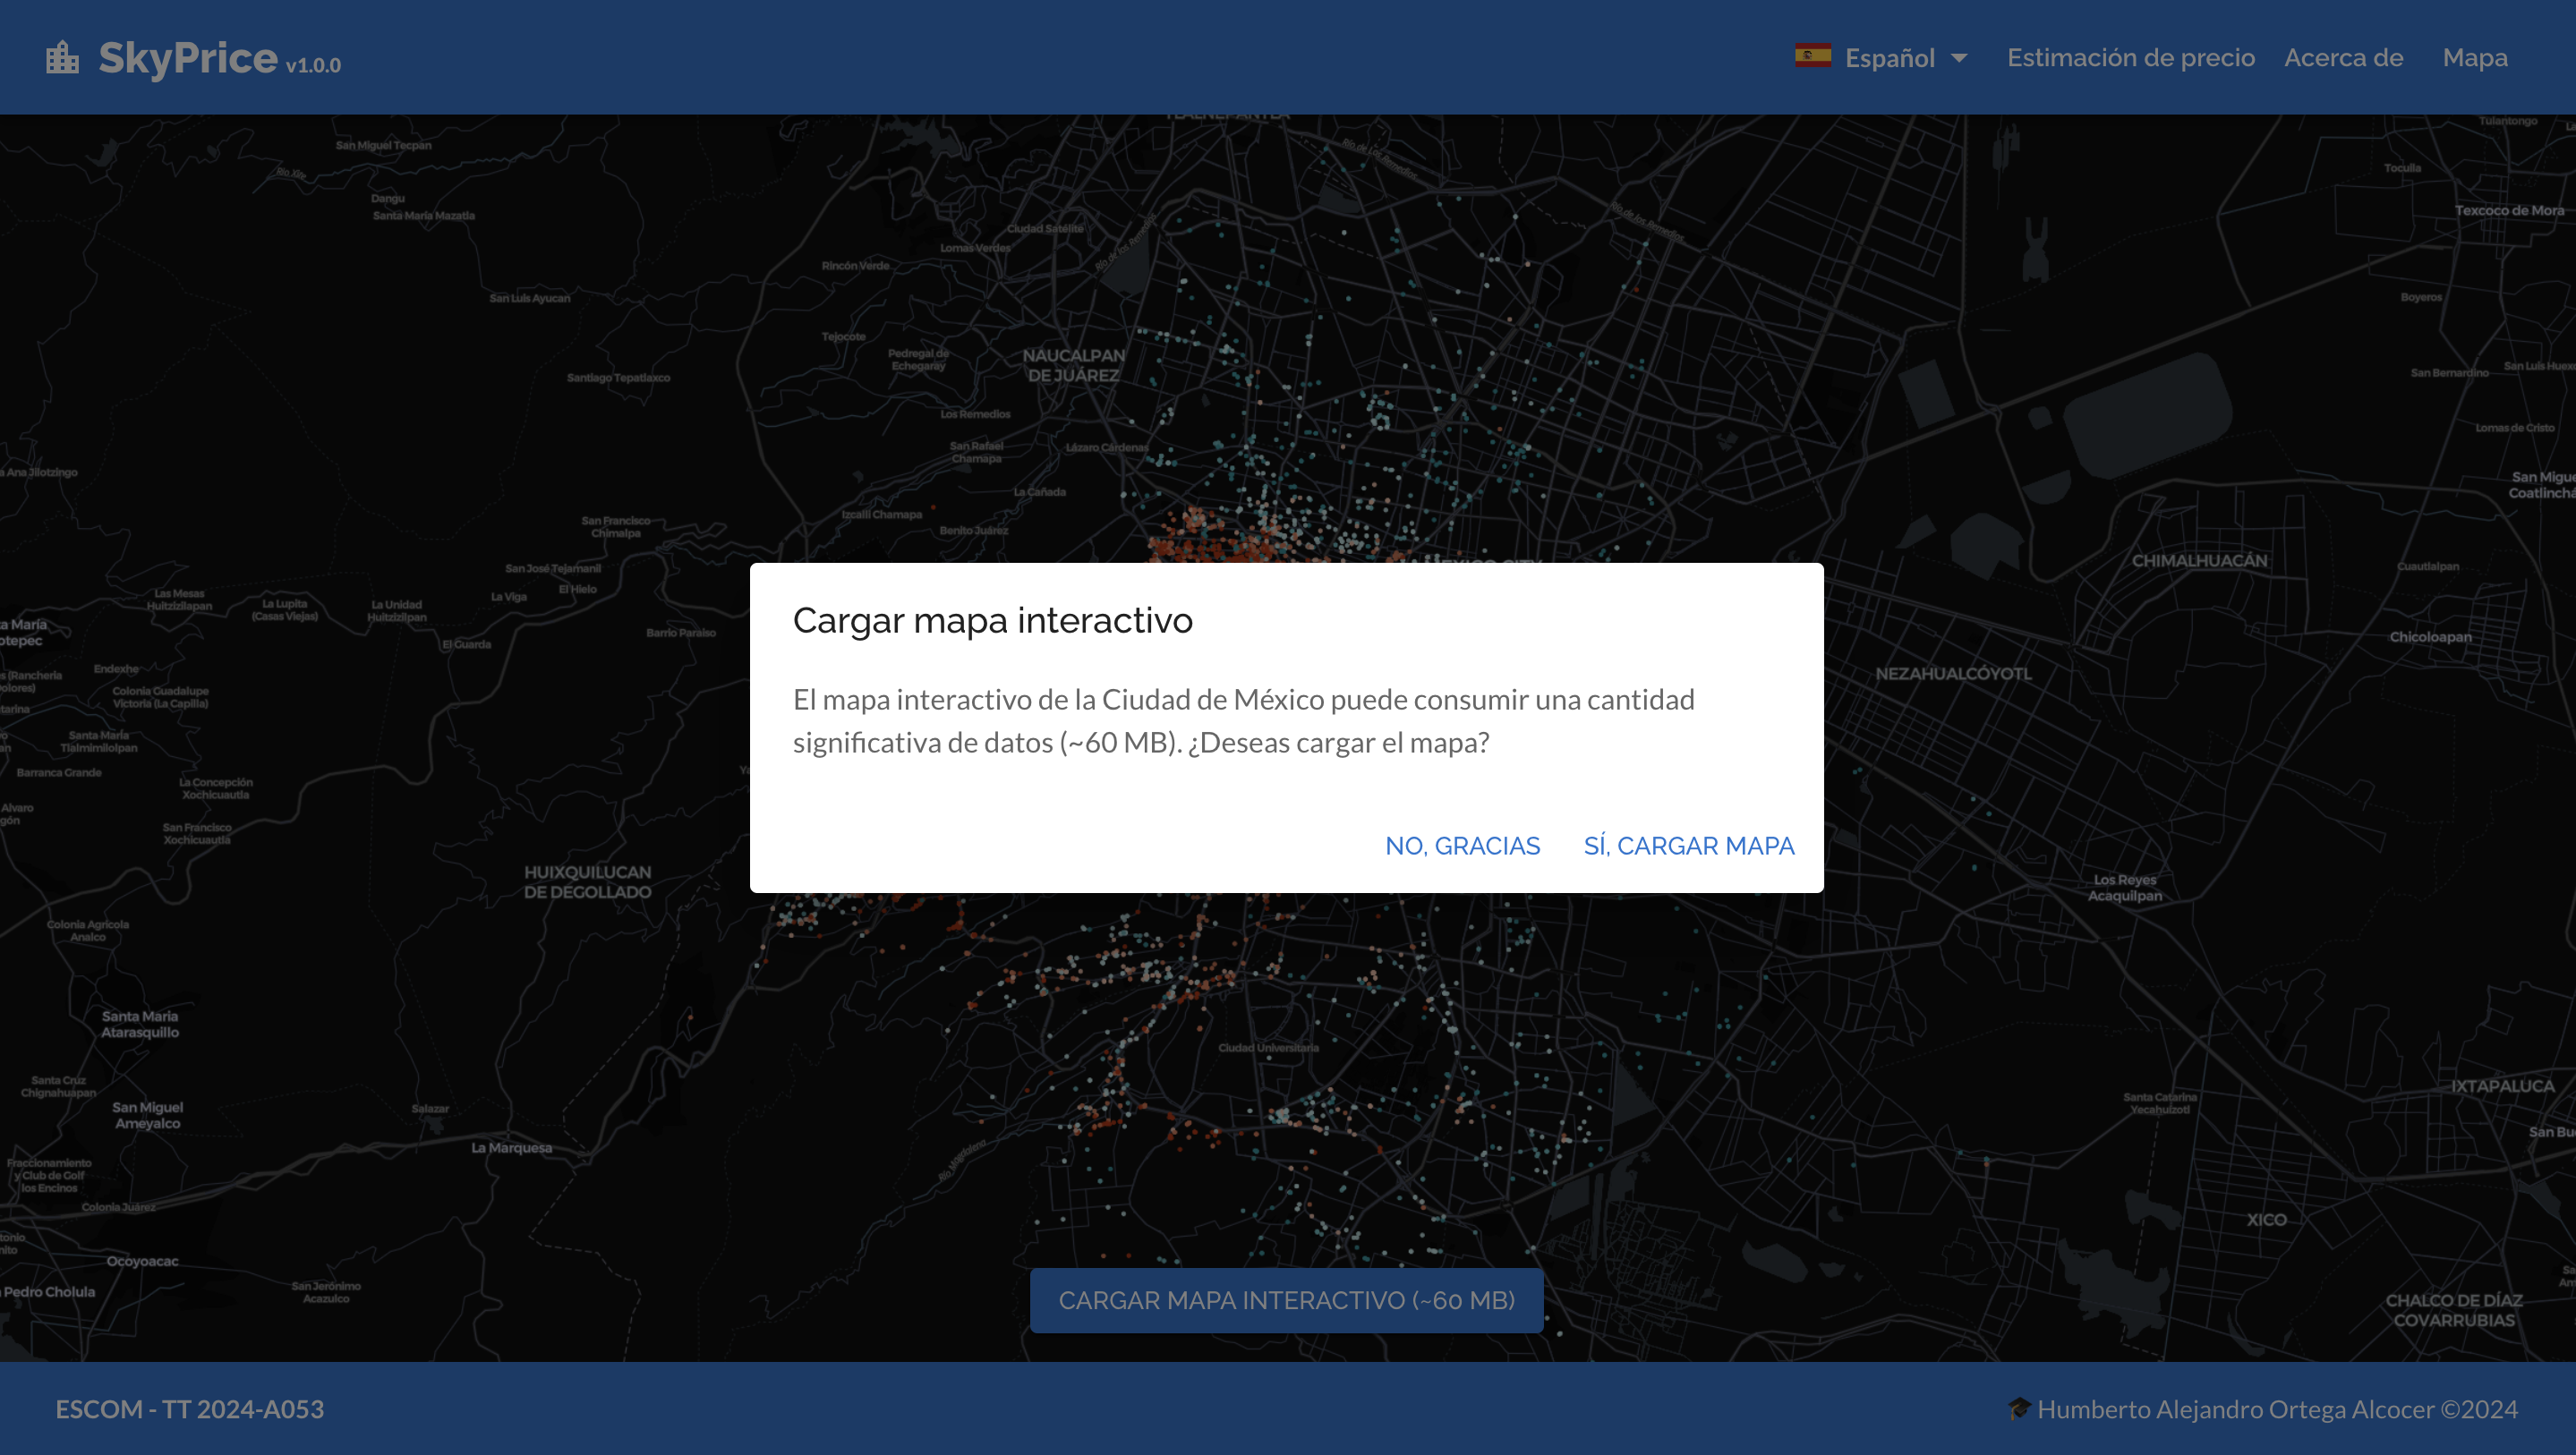
\includegraphics[width=1.0\textwidth]{imagenes/05-implementacion/interfaz-grafica/mapa-interactivo-prompt.png}
    \caption{Página de Mapa interactivo con alerta de carga de datos.}
    \label{fig:mapa-interactivo}
\end{figure}

Si el usuario decide no cargar el mapa dinámico, se muestra la imagen presente en
la figura \ref{fig:mapa-interactivo} y se muestra un botón para cargar el mapa
dinámico. En caso de que el usuario decida cargar el mapa dinámico, se muestra el
mapa interactivo con las capas de datos correspondientes. En la figura
\ref{fig:mapa-interactivo-cargado} se muestra el mapa interactivo con la capa
de datos de propiedades en la Ciudad de México.

\begin{figure}[H]
    \centering
    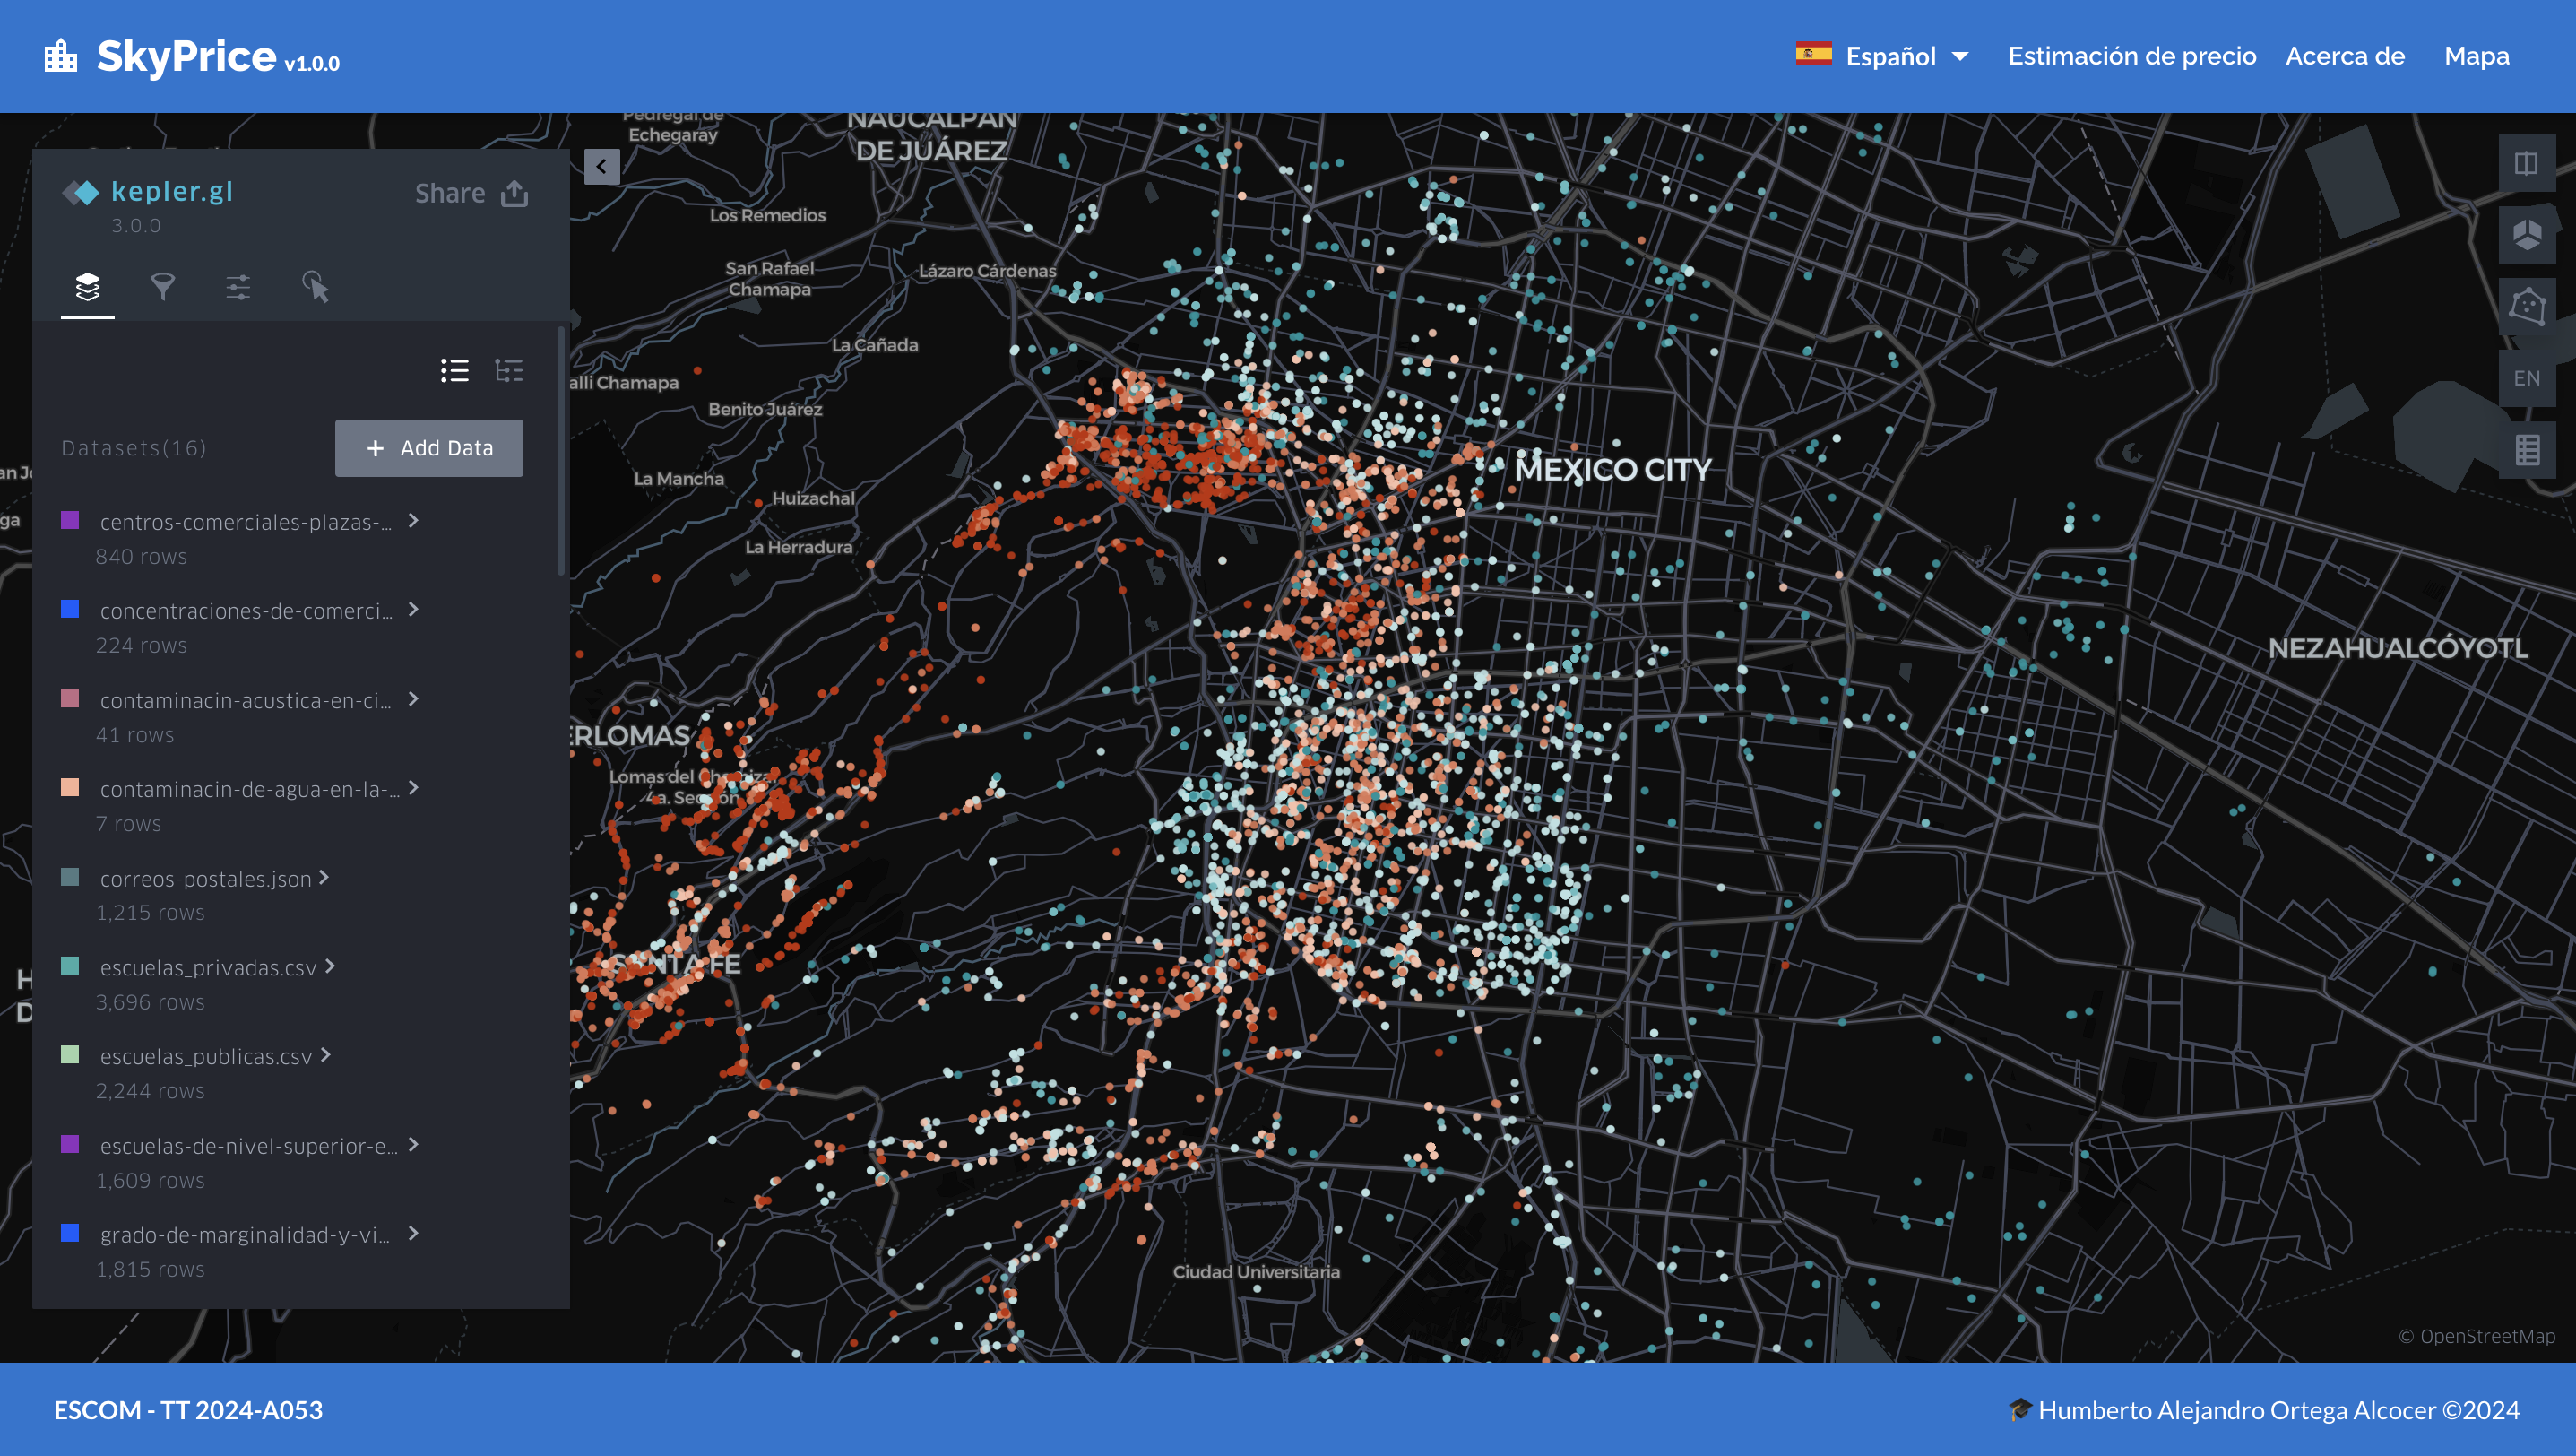
\includegraphics[width=1.0\textwidth]{imagenes/05-implementacion/interfaz-grafica/mapa-interactivo-cargado.png}
    \caption{Página de Mapa interactivo con capa de datos de propiedades en la Ciudad de México.}
    \label{fig:mapa-interactivo-cargado}
\end{figure}

Kepler.gl permite a los usuarios interactuar con el mapa, incluyendo la capacidad
de hacer zoom, desplazarse, cambiar la perspectiva, activar y desactivar capas de
datos, entre otras funcionalidades \cite{kepler_gl_docs}. La intención de proveer esta herramienta
junto con capas de datos relevantes es que los usuarios puedan explorar y
visualizar los datos y obtener información valiosa sobre las propiedades en la
Ciudad de México.

En el cuadro \ref{tab:capas-datos} se muestra un resumen de las capas de datos
disponibles en el mapa interactivo, incluyendo la fuente de los datos y una breve
descripción de cada capa.

\begin{table}[H]
    \centering
    \begin{tabular}{|p{0.3\textwidth}|p{0.6\textwidth}|}
    \hline
    \rowcolor{azulclaro}
    \textbf{Capa de datos} & \textbf{Descripción} \\ \hline
    Departamentos & Conjunto de datos del proyecto \\ \hline
    Centros y plazas comerciales y tiendas de autoservicios \cite{cdmx_centros_comerciales} & Centros y plazas comerciales y tiendas de autoservicios en la Ciudad de México \\ \hline
    Concentraciones comerciantes \cite{cdmx_concentraciones_comerciantes} & Concentraciones de comerciantes en la Ciudad de México \\ \hline
    Contaminación acústica \cite{cdmx_contaminacion_acustica} & Contaminación acústica en la Ciudad de México \\ \hline
    Contaminación del agua \cite{cdmx_contaminacion_agua} & Contaminación del agua en la Ciudad de México  \\ \hline
    Códigos postales \cite{cdmx_codigos_postales} & Códigos postales en la Ciudad de México  \\ \hline
    Escuelas privadas \cite{cdmx_escuelas_privadas} & Escuelas privadas en la Ciudad de México  \\ \hline
    Escuelas públicas \cite{cdmx_escuelas_publicas} & Escuelas públicas en la Ciudad de México  \\ \hline
    Escuelas de nivel superior \cite{cdmx_escuelas_superior} & Escuelas de nivel superior en la Zona Metropolitana del Valle de México  \\ \hline
    Grado de marginalidad y violencia \cite{cdmx_marginalidad_violencia} & Grado de marginalidad y violencia en la Ciudad de México  \\ \hline
    Hospitales y centros de salud \cite{cdmx_hospitales_salud} & Hospitales y centros de salud en la Ciudad de México  \\ \hline
    Alcaldías \cite{cdmx_alcaldias} & Alcaldías en la Ciudad de México \\ \hline
    Mercados \cite{cdmx_mercados_publicos} & Mercados públicos en la Ciudad de México  \\ \hline
    Estaciones de Metro \cite{cdmx_lineas_metro} & Estaciones de Metro en la Ciudad de México \\ \hline
    Epicentros de sismos \cite{cdmx_sismos} & Epicentros de sismos en la Ciudad de México \\ \hline
    Tianguis \cite{cdmx_tianguis} & Tianguis en la Ciudad de México  \\ \hline
    \end{tabular}
    \caption{Capas de datos disponibles en el mapa interactivo.}
    \label{tab:capas-datos}
\end{table}

Estos conjuntos de datos no son definitivos, una de las ventajas de Kepler.gl es
que permite a los usuarios cargar sus propios datos y visualizarlos en el mapa
interactivo, lo que facilita la exploración y el análisis de datos geoespaciales.
A su vez, la capacidad de Kepler.gl para exportar datos y visualizaciones permite
a los usuarios compartir y colaborar en proyectos de datos geoespaciales.

Para demostrar una posibilidad de uso, en la figura \ref{fig:mapa-interactivo-ejemplo}
se muestra el mapa interactivo con  la capa de datos de propiedades en la Ciudad
de México, la capa con las Alcaldías y la capa de contaminación acústica, que podrían
ser útiles para analizar la relación entre el precio de las propiedades y la contaminación
acústica en la Ciudad de México.

\begin{figure}[H]
    \centering
    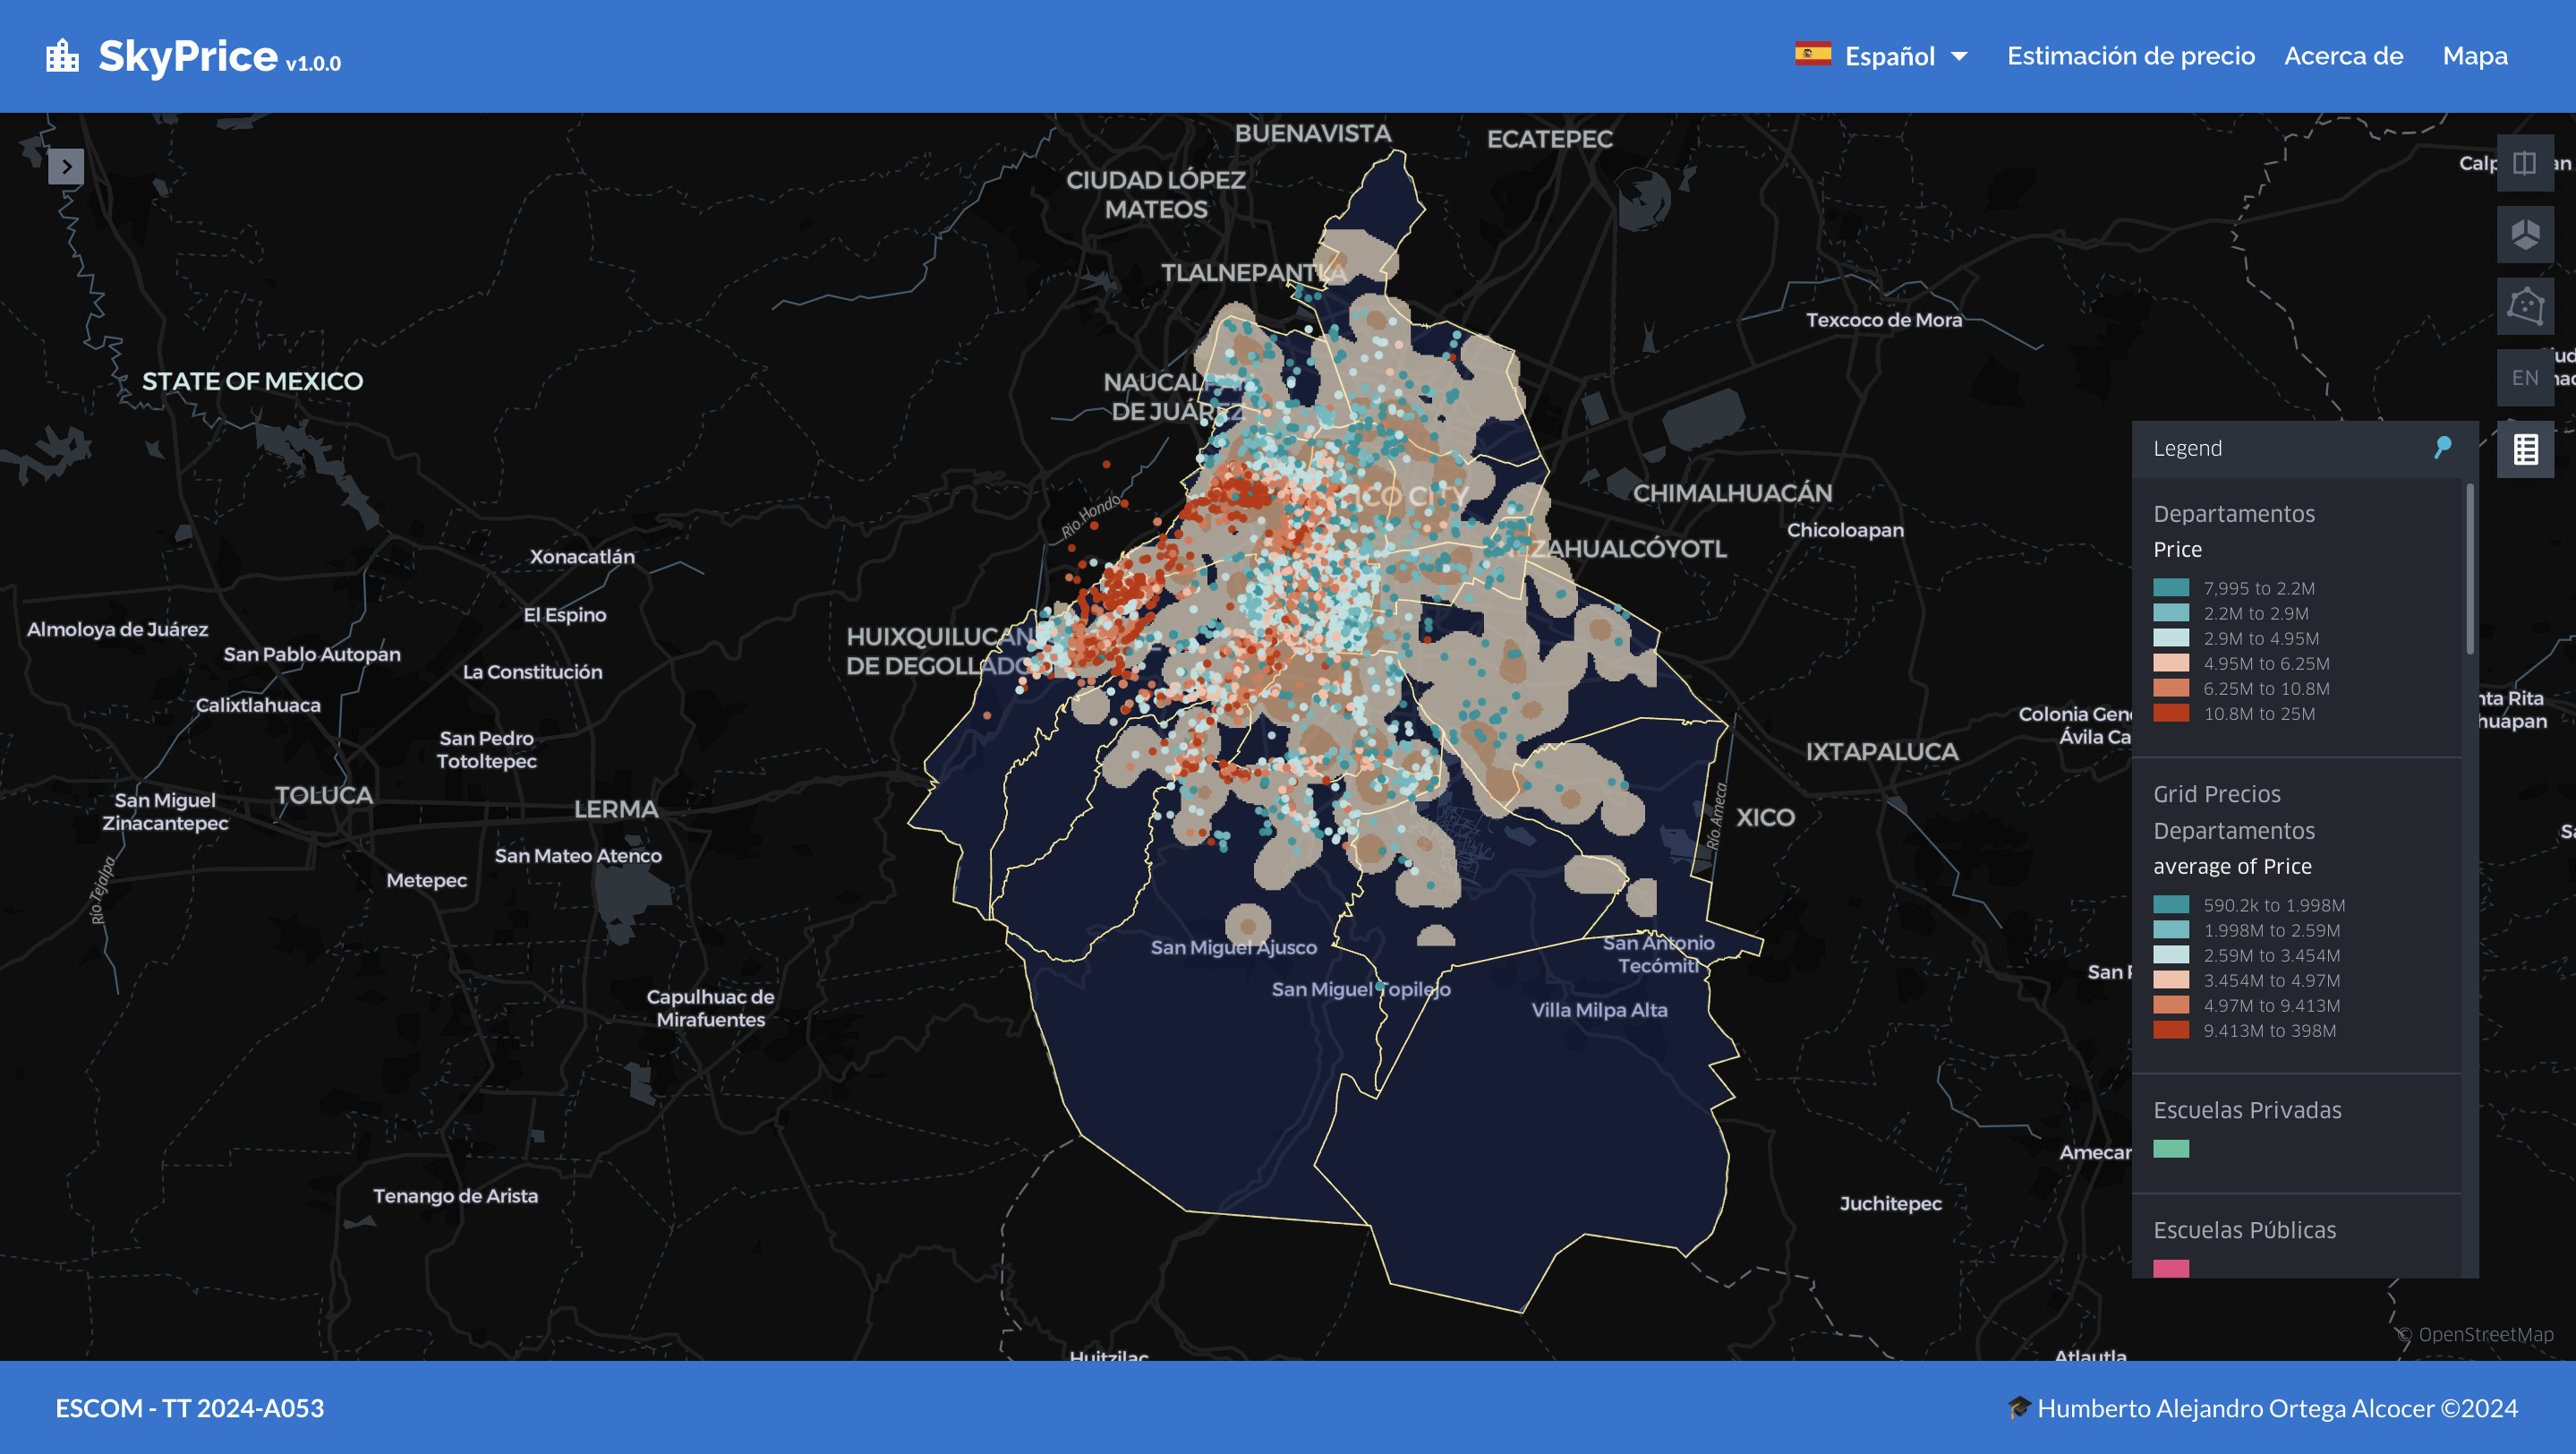
\includegraphics[width=1.0\textwidth]{imagenes/05-implementacion/interfaz-grafica/mapa-interactivo-ejemplo.png}
    \caption{Mapa interactivo con capa de datos de propiedades, alcaldías y contaminación acústica.}
    \label{fig:mapa-interactivo-ejemplo}
\end{figure}

\subsection{Diseño responsivo}
A bien de garantizar una experiencia de usuario óptima en dispositivos móviles y
tabletas, se implementó un diseño responsivo en la interfaz gráfica. El diseño
responsivo se logró utilizando Media Queries de CSS y la biblioteca Material-UI,
la cual proporciona componentes y estilos responsivos para aplicaciones web.

En la Figura \ref{fig:main-responsive} se muestra la pantalla principal de la
interfaz gráfica en diseño móvil, con el menú de hamburguesa desplegado mostrando
así las opciones de navegación. En la Figura \ref{fig:results-responsive} se
muestra la pantalla de resultados de la interfaz gráfica en diseño móvil, con
las predicciones de los modelos de aprendizaje automático.

\begin{figure}[H]
    \centering
    \begin{minipage}{0.45\textwidth}
        \centering
        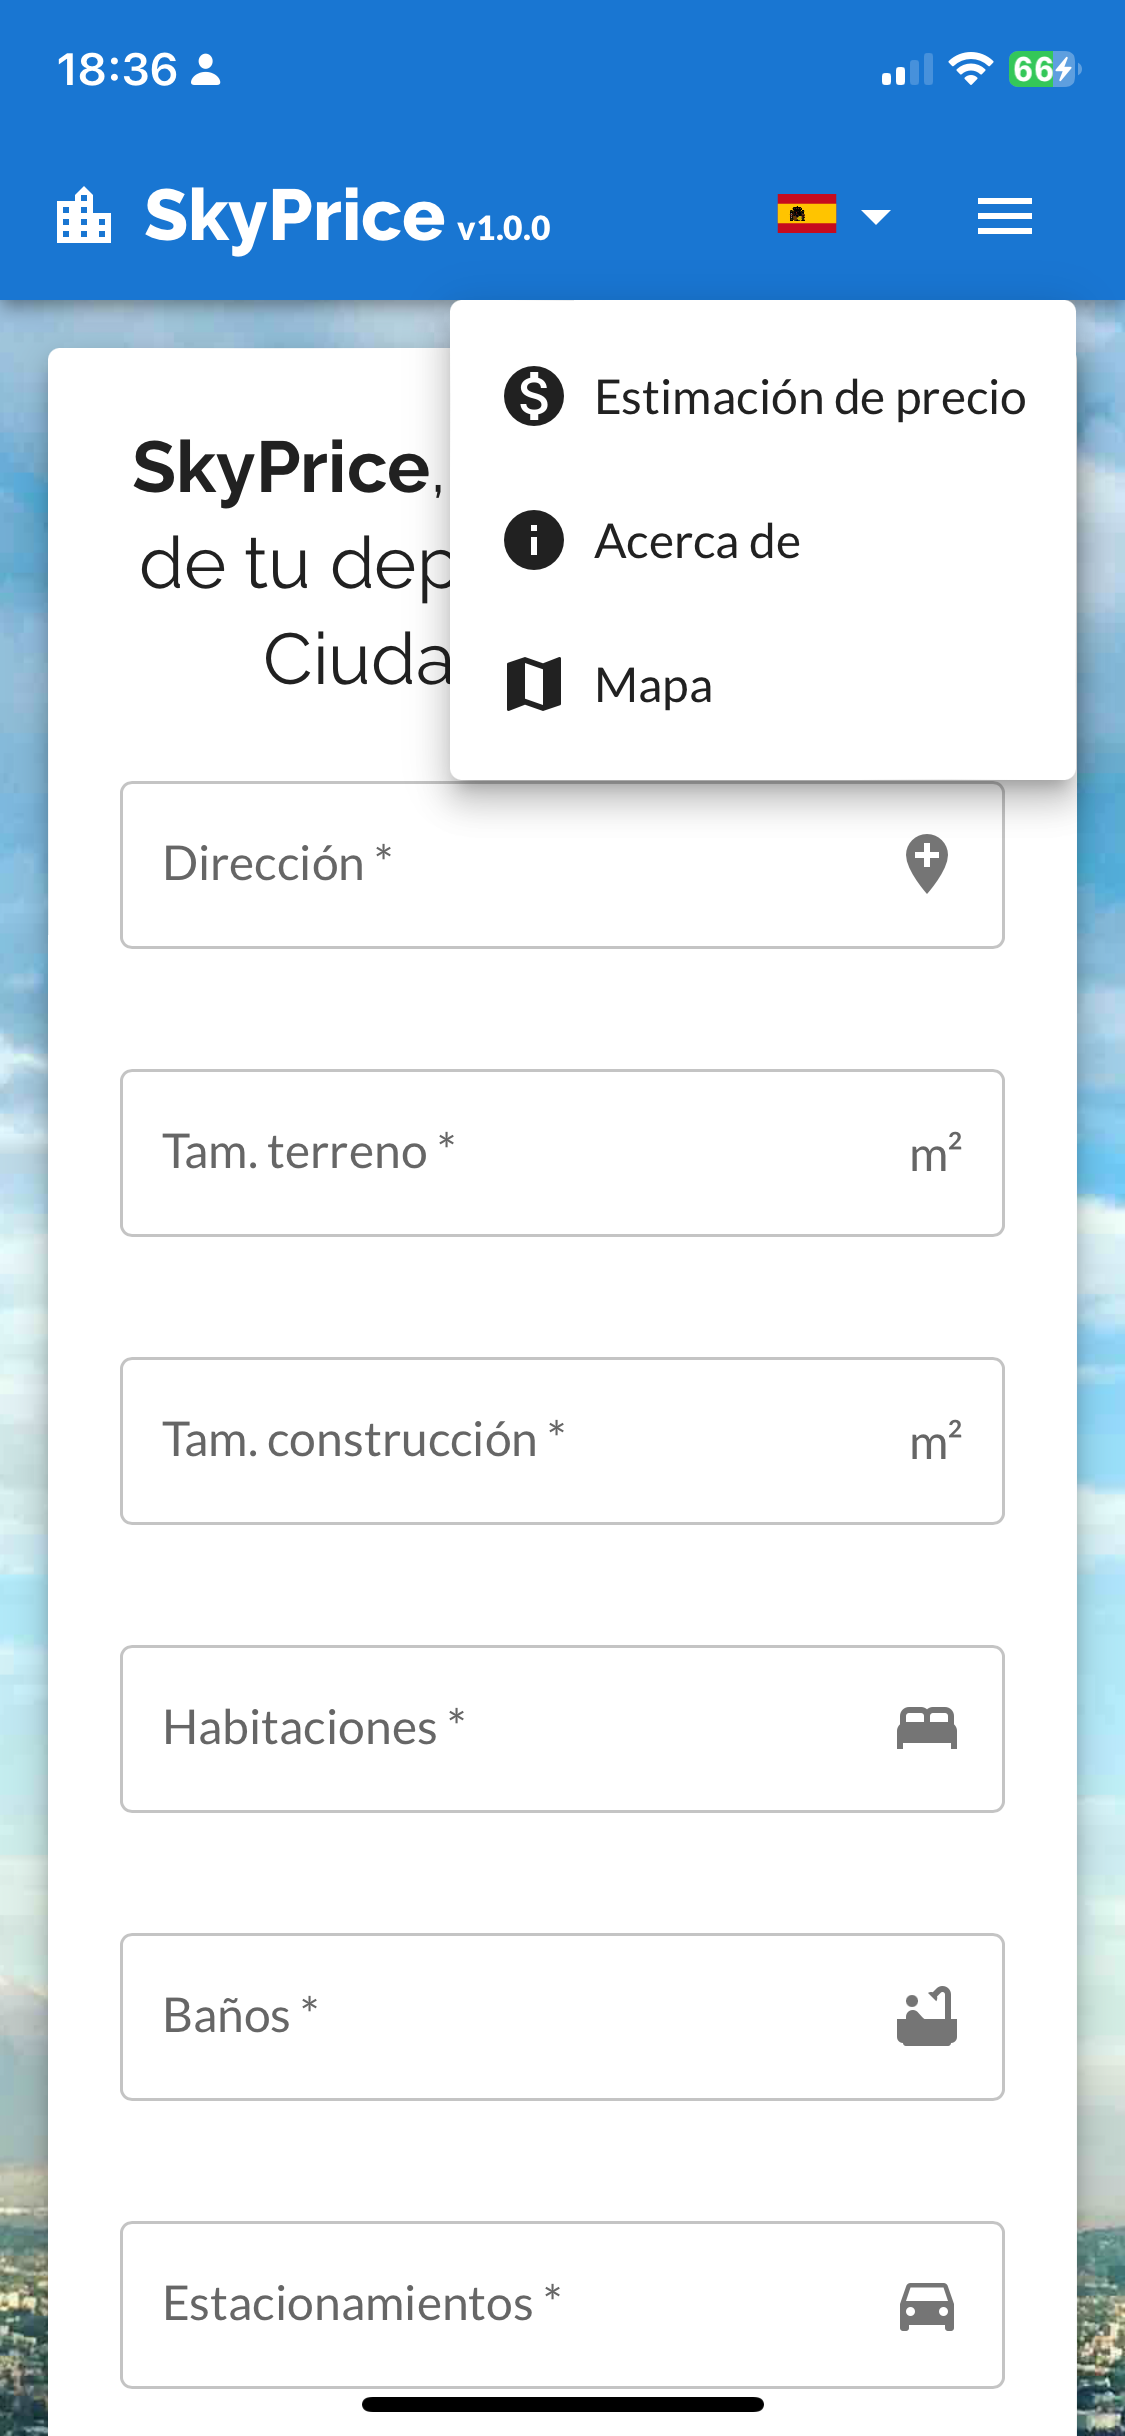
\includegraphics[width=\textwidth]{imagenes/05-implementacion/interfaz-grafica/main-responsive.png}
        \caption{Pantalla principal en diseño móvil}
        \label{fig:main-responsive}
    \end{minipage}\hfill
    \begin{minipage}{0.45\textwidth}
        \centering
        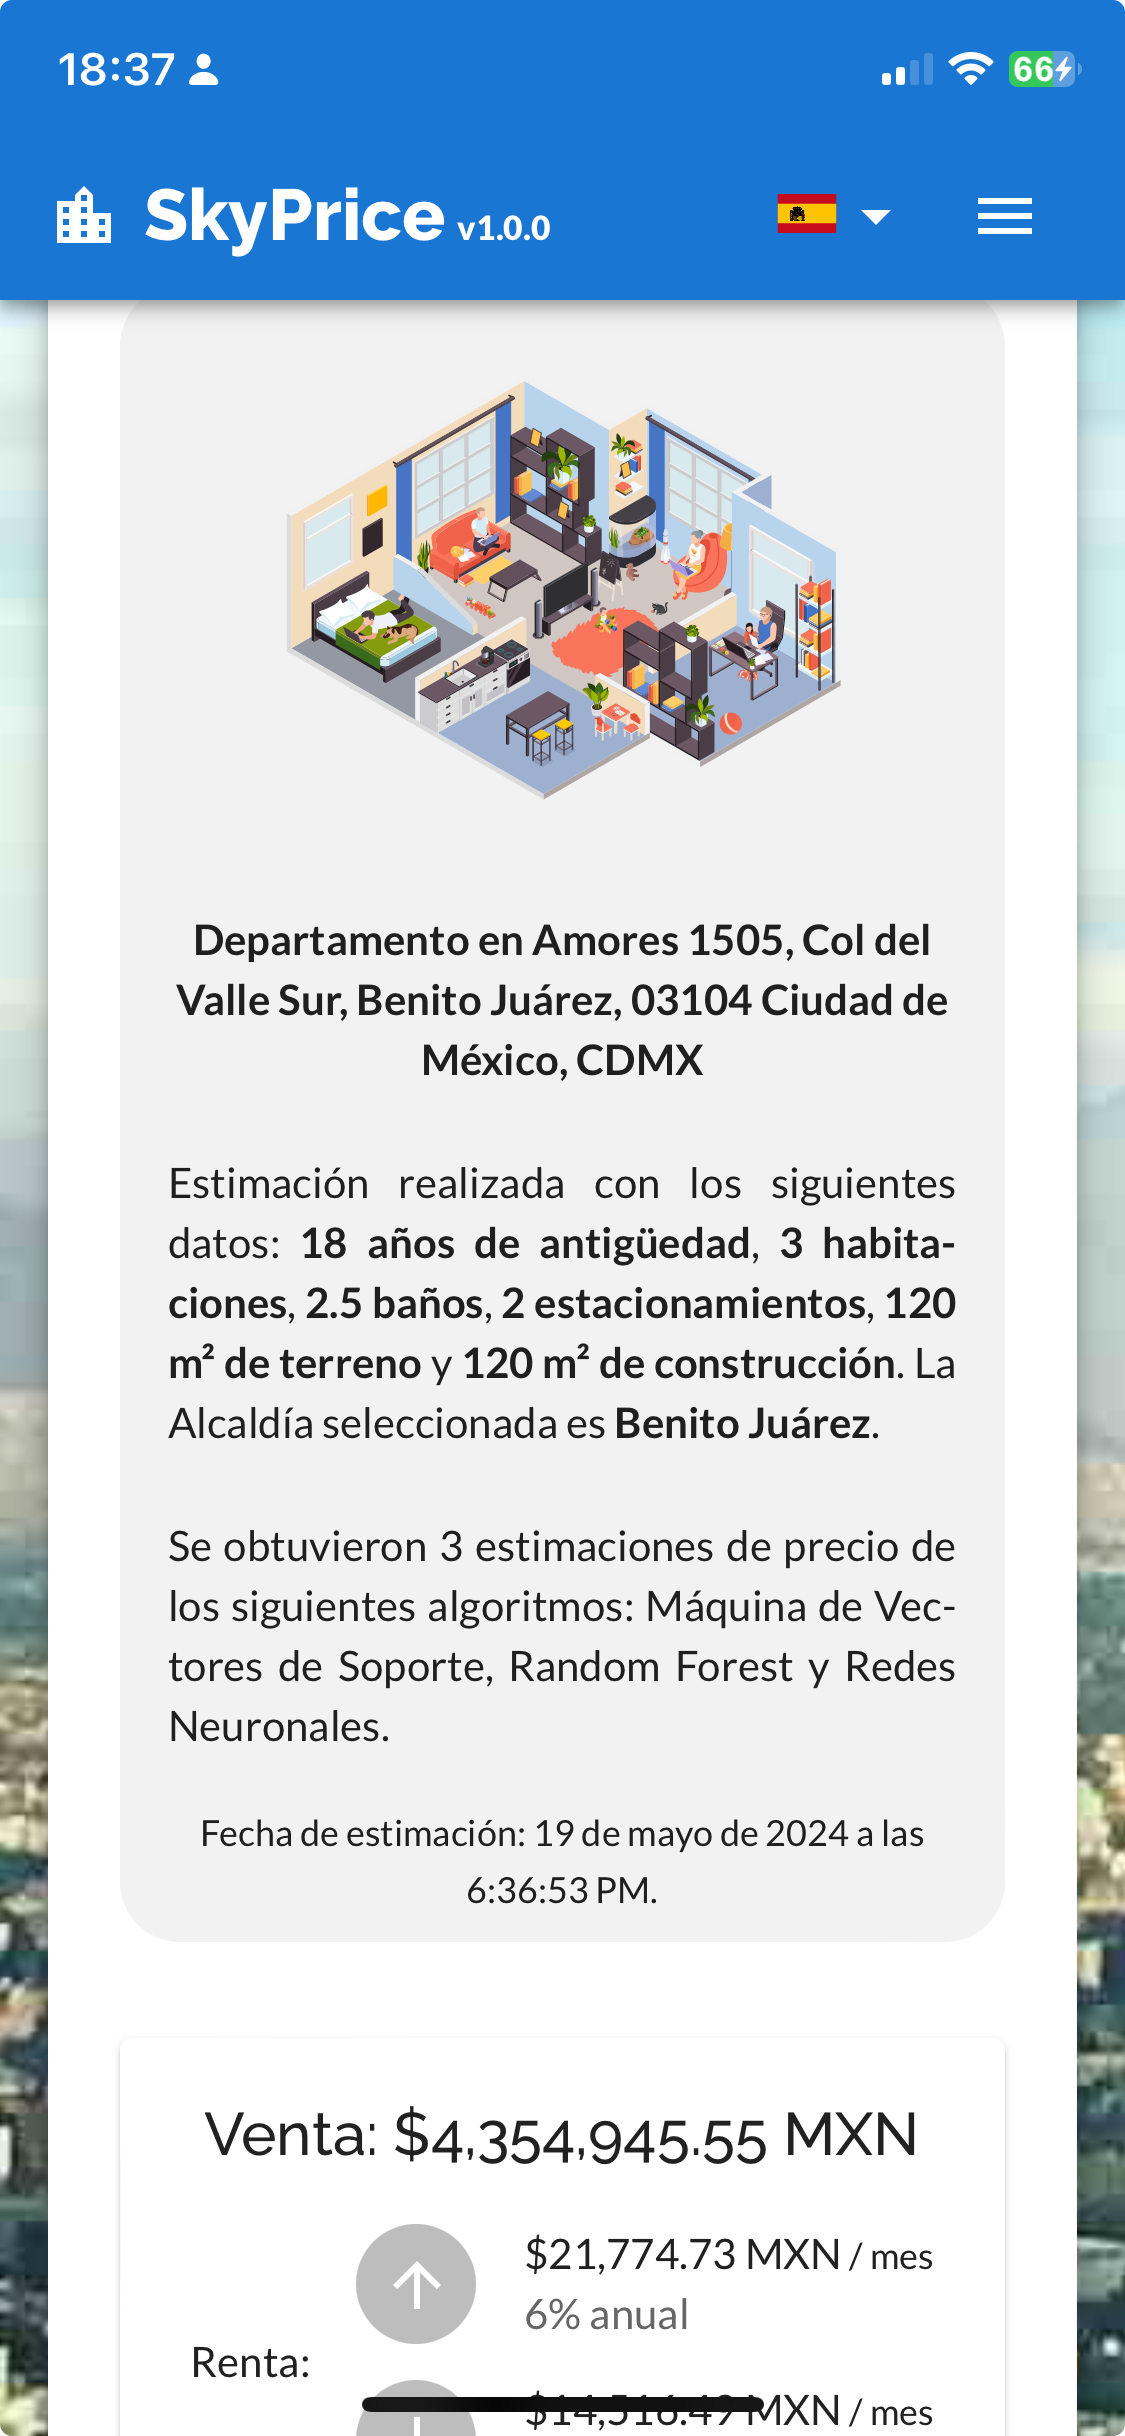
\includegraphics[width=\textwidth]{imagenes/05-implementacion/interfaz-grafica/resultados-responsive.jpeg}
        \caption{Pantalla de resultados en diseño móvil}
        \label{fig:results-responsive}
    \end{minipage}
\end{figure}

En la Figura \ref{fig:about-responsive} se muestra la pantalla de Acerca de en
diseño móvil, con la gráfica de comparación de métricas de evaluación de los
modelos de aprendizaje automático. En la Figura \ref{fig:map-responsive} se
muestra la pantalla de Mapa interactivo en diseño móvil, con la capa de datos
de propiedades en la Ciudad de México.

\begin{figure}[H]
    \centering
    \begin{minipage}{0.45\textwidth}
        \centering
        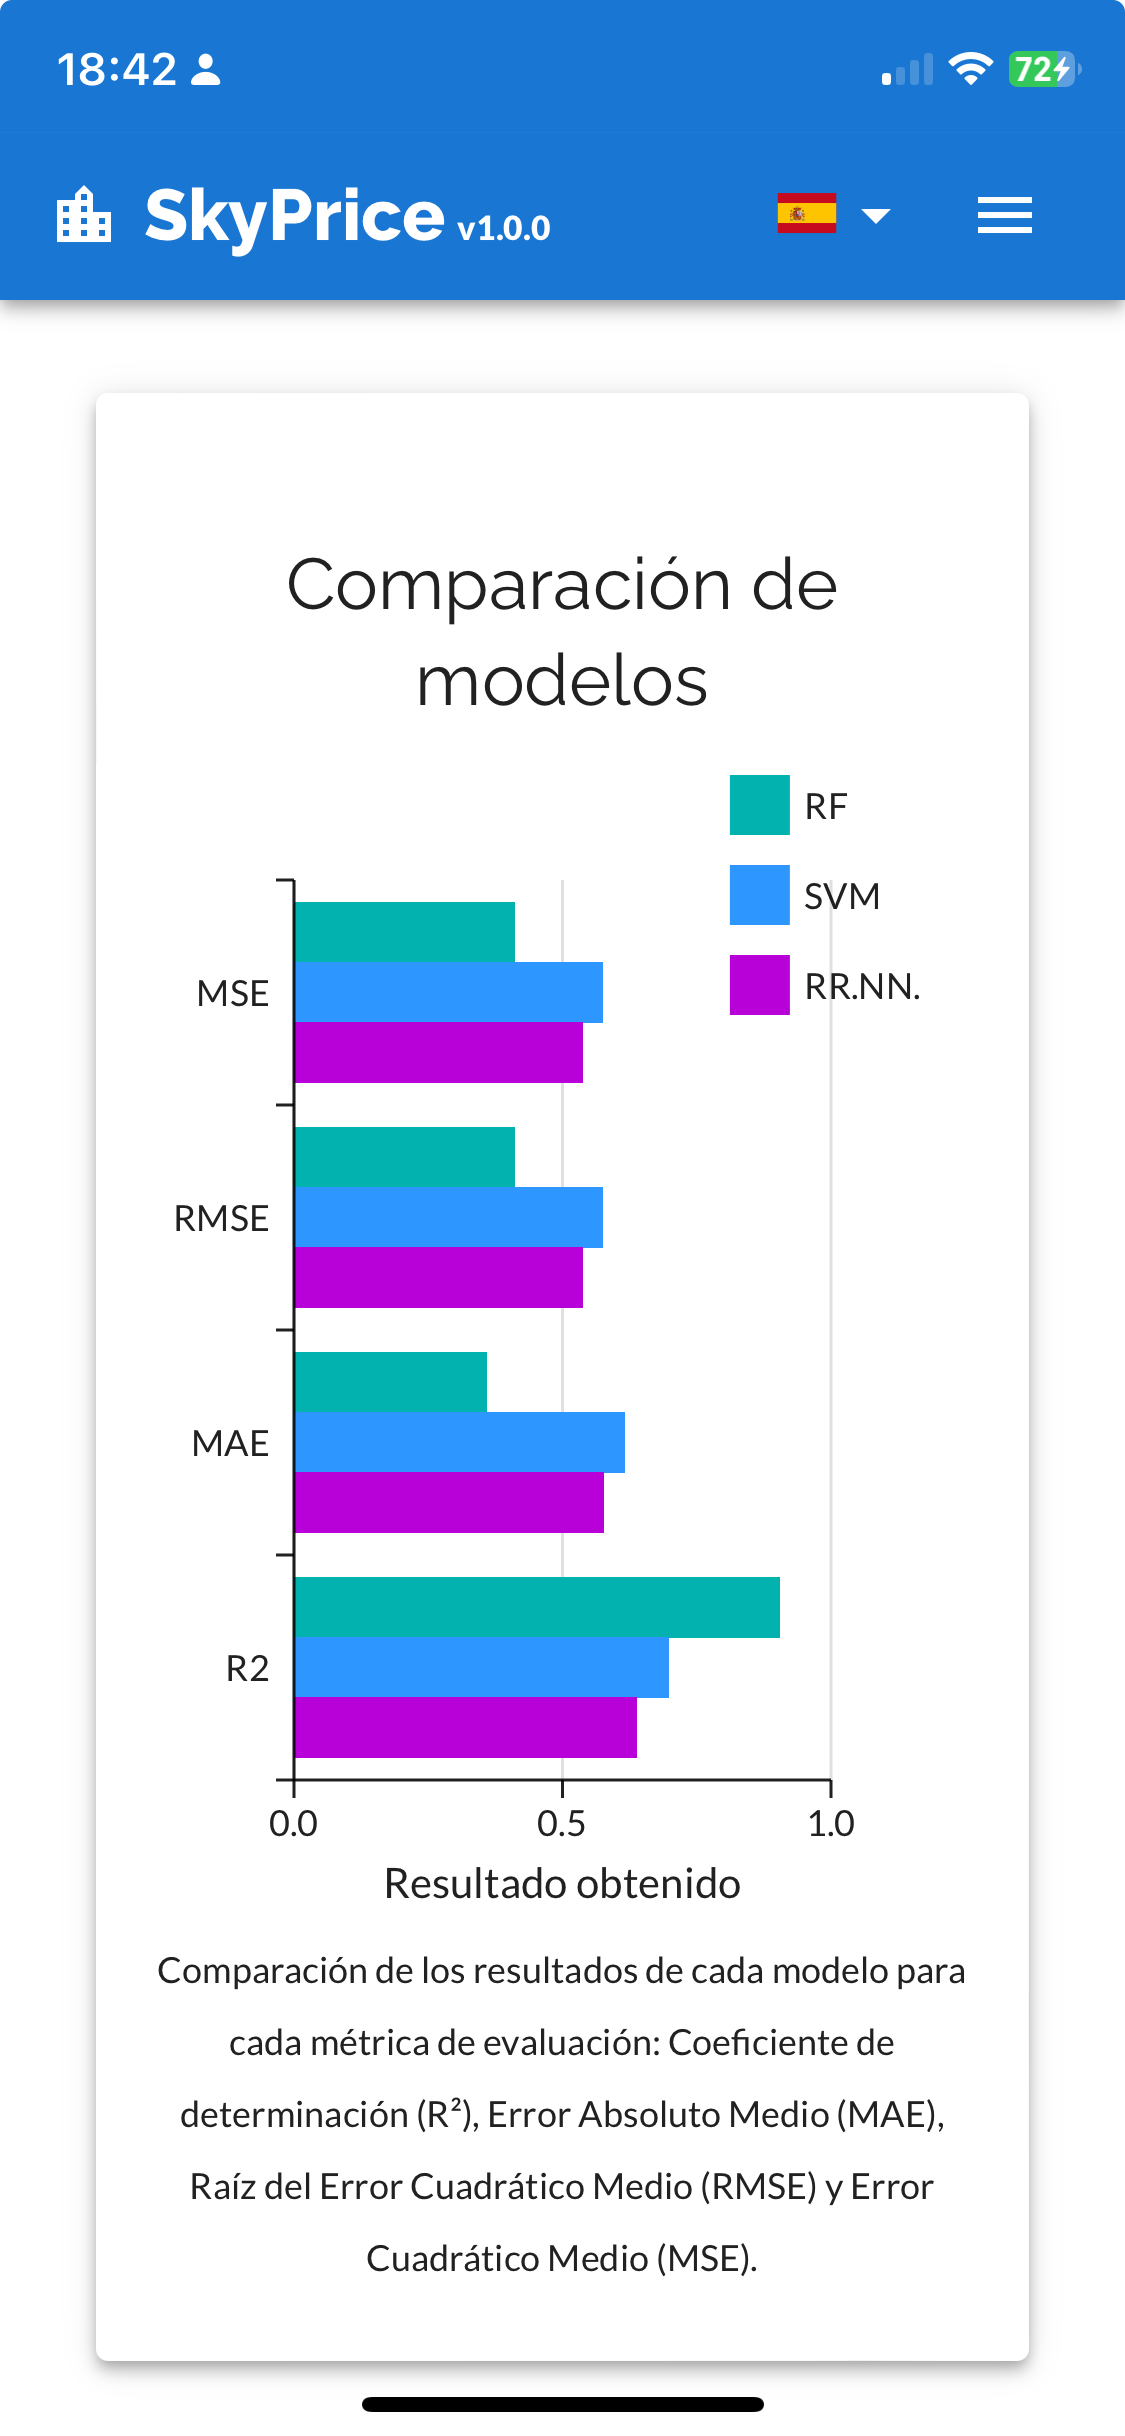
\includegraphics[width=\textwidth]{imagenes/05-implementacion/interfaz-grafica/modelos-responsive.jpeg}
        \caption{Pantalla de Acerca de en diseño móvil}
        \label{fig:about-responsive}
    \end{minipage}\hfill
    \begin{minipage}{0.45\textwidth}
        \centering
        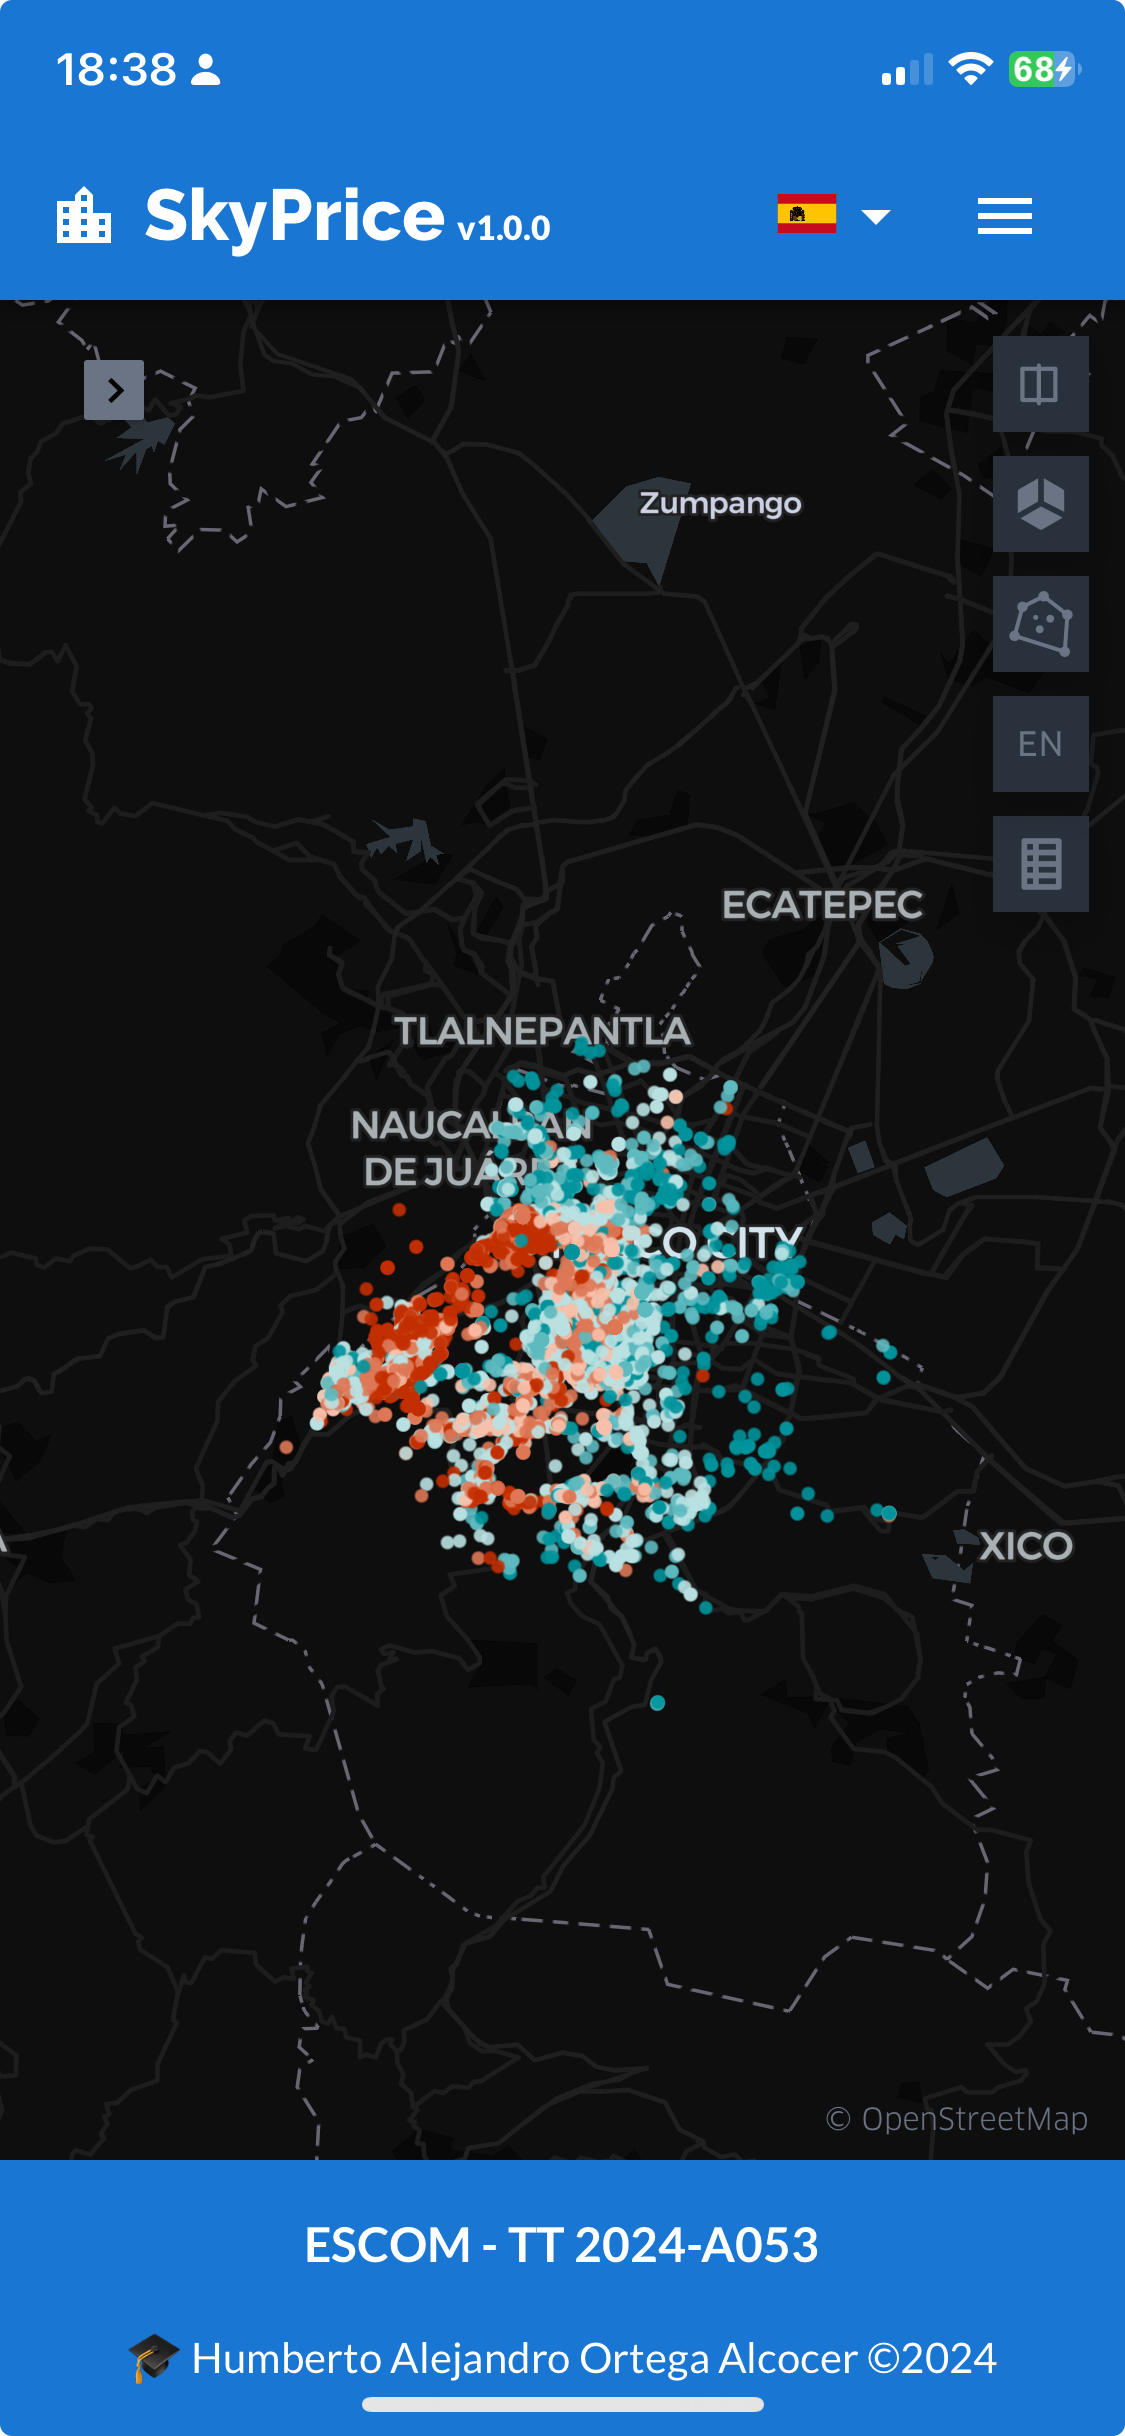
\includegraphics[width=\textwidth]{imagenes/05-implementacion/interfaz-grafica/mapa-responsive.jpeg}
        \caption{Pantalla de Mapa interactivo en diseño móvil}
        \label{fig:map-responsive}
    \end{minipage}
\end{figure}

\section{Despliegue en la nube}
El despliegue en la nube del servicio web y la interfaz gráfica se llevó a cabo
utilizando Amazon Web Services (AWS), para esto se utilizó una cuenta de AWS Educate
que proporciona créditos y recursos para estudiantes y educadores \cite{aws_educate}.

Lo primero que se realizó fue la adquisición de un dominio para la aplicación,
posteriormente se empaquetó y distribuyó el servicio web utilizando contenedores
Docker, se desplegó el servicio web en AWS Elastic Beanstalk y la interfaz gráfica
en AWS S3.

\subsection{Dominio}
Se llevó a cabo la adquisición de un dominio para la aplicación. Este dominio
se eligió a partir de la disponibilidad, relevancia al tema del presente
trabajo terminal y costo. El dominio elegido fue \texttt{skyprice.xyz}.

Para llevar a cabo la compra del dominio, se utilizó el servicio de
\textit{Namecheap}, el cual ofrece una interfaz amigable y opciones de
configuración avanzadas \cite{namecheap}. La compra del dominio se realizó sin problemas y, en
la figura \ref{fig:skyprice-xyz} se muestra la información del dominio en el
panel de control de \textit{Namecheap}.

\begin{figure}[H]
    \centering
    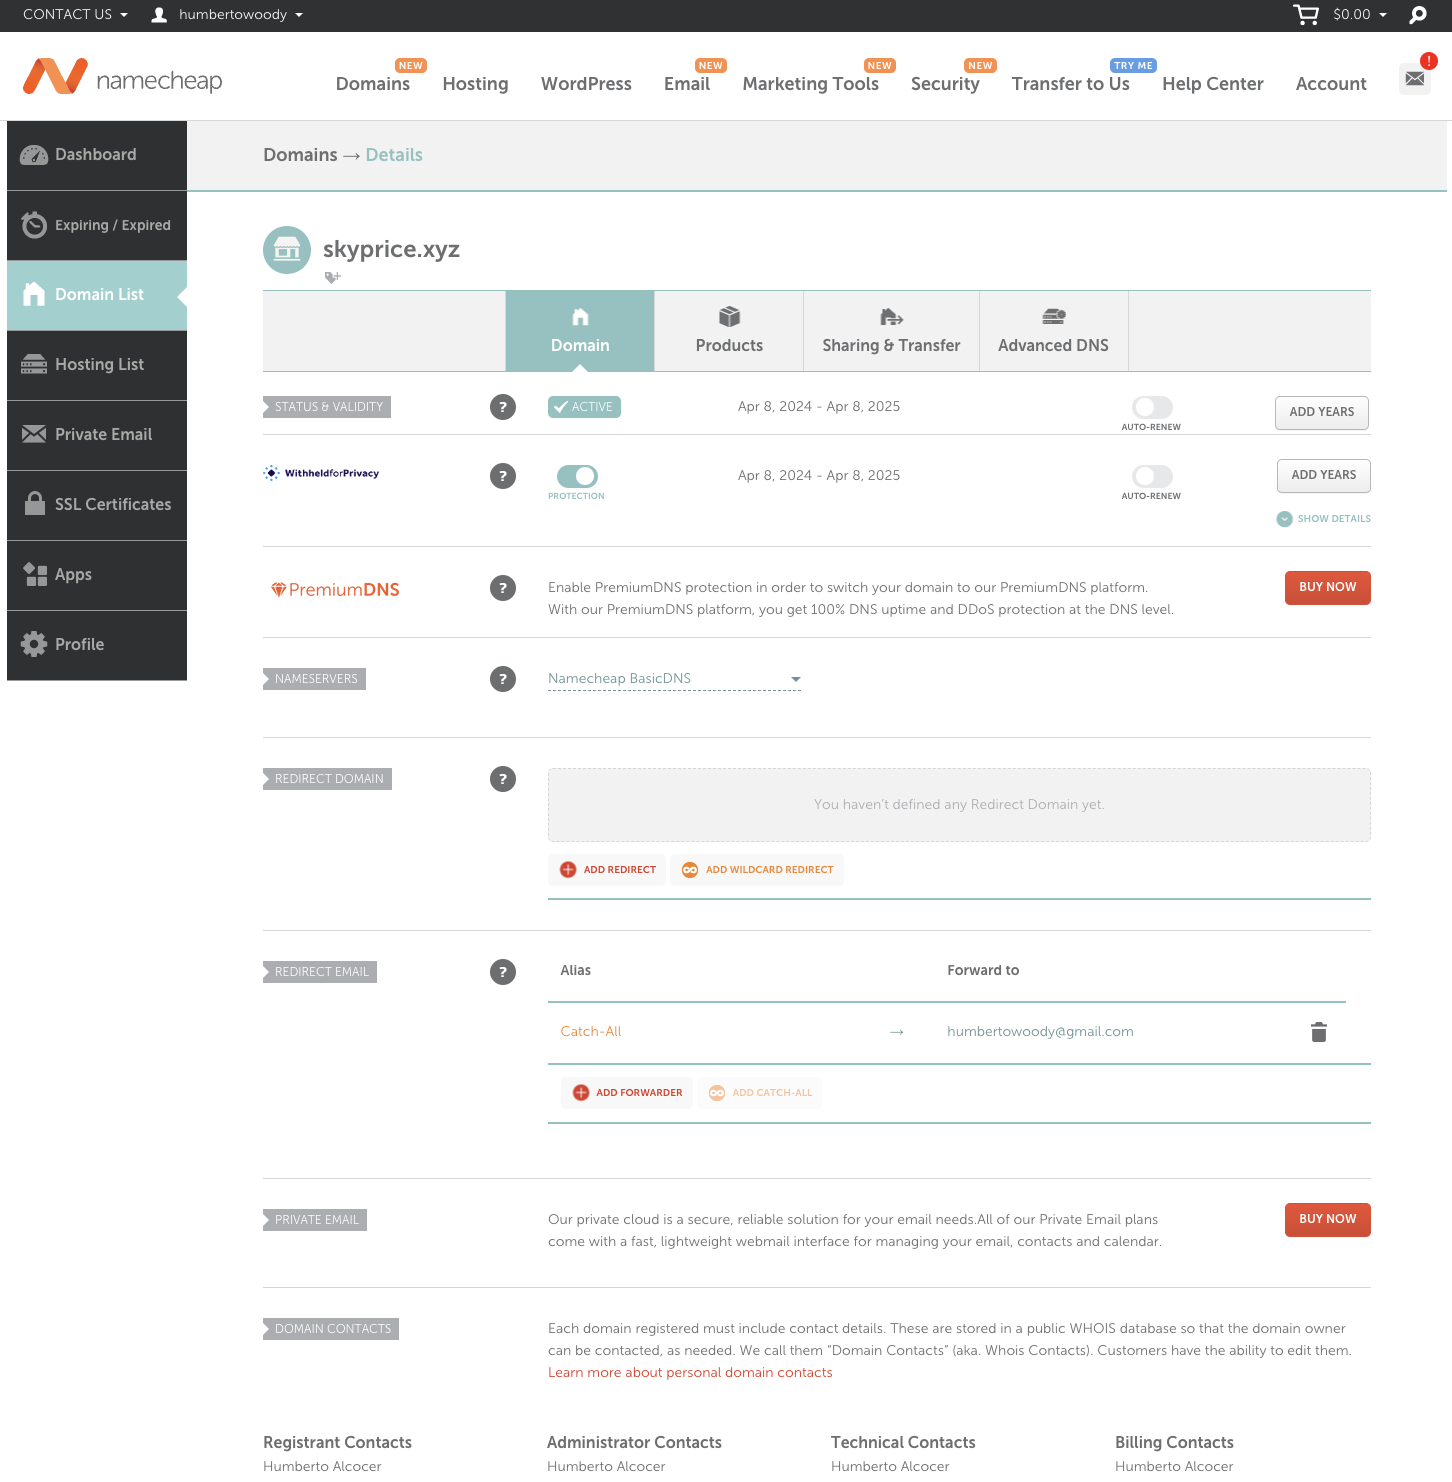
\includegraphics[width=0.8\textwidth]{imagenes/05-implementacion/despliegue/namecheapskypricexyz.png}
    \caption{Información del dominio \texttt{skyprice.xyz} en Namecheap.}
    \label{fig:skyprice-xyz}
\end{figure}

\subsubsection{AWS Route 53}
Inicialmente se contemplaba realizar la adquisición del dominio directamente
en AWS, sin embargo, debido a que Route53 no ofrece dominios con extensión
\texttt{.xyz}, se optó por adquirir el dominio en Namecheap y posteriormente
configurar los registros DNS en Route53.

En el cuadro \ref{tab:registros-dns} se muestra un resumen de los registros DNS
configurados en AWS Route 53 para el dominio \texttt{skyprice.xyz}.

\begin{table}[H]
    \centering
    \begin{tabular}{|p{0.3\textwidth}|p{0.2\textwidth}|p{0.4\textwidth}|}
    \hline
    \rowcolor{azulclaro}
      \textbf{Nombre} & \textbf{Tipo} & \textbf{Valor} \\ \hline
      \texttt{api.skyprice.xyz} & \texttt{CNAME} & DNS de Elastic Beanstalk \\ \hline
      \texttt{www.skyprice.xyz} & \texttt{CNAME} & DNS de CloudFront \\ \hline
      \texttt{skyprice.xyz} & \texttt{CNAME} & DNS de CloudFront \\ \hline
    \end{tabular}
    \caption{Registros DNS configurados en AWS Route 53 para el dominio \texttt{skyprice.xyz}.}
    \label{tab:registros-dns}
\end{table}

\subsection{Empaque y distribución del servicio web}

Uno de los aspectos más importantes de la implementación de cualquier sistema de software es la distribución del mismo. En este caso, se optó por utilizar contenedores Docker para empaquetar y distribuir el servicio web.

En este sentido, se creó un \textit{Dockerfile} que puede observarse en el listado \ref{lst:dockerfile}, el cual define la configuración y las dependencias necesarias (a nivel de sistema operativo y de software) para ejecutar el servicio. Posteriormente, se construyó una imagen Docker a partir de este archivo, la cual se publicó en un repositorio de imágenes, en este caso, Docker Hub.

De esta manera, se asegura que la misma configuración se utilice en cualquier entorno (local o en la nube), lo que facilita el desarrollo, las pruebas y el despliegue del servicio web.

En particular, Amazon Web Services (AWS) Elastic Beanstalk fue el servicio utilizado para desplegar el servicio web en la nube. Elastic Beanstalk permite utilizar imágenes Docker alojadas en Docker Hub, lo que facilita llevar cambios a producción de manera rápida y segura.

\begin{lstlisting}[language=dockerfile, caption={Dockerfile para el servicio web}, label={lst:dockerfile}]
# Usar una imagen oficial de Python como imagen base
FROM python:3.12-slim as builder

# Actualizar el sistema e instalar dependencias necesarias para SciPy, Scikit-learn, TensorFlow, Keras, etc.
RUN apt-get update && apt-get install -y --no-install-recommends \
    build-essential \
    libblas-dev \
    liblapack-dev \
    libatlas-base-dev \
    gfortran \
    libhdf5-dev \
    libfreetype6-dev \
    libpng-dev \
    libzmq3-dev \
    pkg-config \
    software-properties-common \
    swig \
    curl \
    git \
    g++ \
    gcc \
    && apt-get clean \
    && rm -rf /var/lib/apt/lists/*

# Establecer el directorio de trabajo en el contenedor
WORKDIR /app

# Copiar Pipfile y Pipfile.lock al contenedor
COPY Pipfile Pipfile.lock /app/

# Instalar pipenv y las dependencias del proyecto
RUN pip install --upgrade pip pipenv && \
    pipenv install --system --deploy

# Copiar el resto del código de la aplicación al contenedor
COPY . /app

# Etapa final
FROM python:3.12-slim as run

# Copiar los archivos de la etapa anterior
COPY --from=builder /usr/local/lib/python3.12/site-packages /usr/local/lib/python3.12/site-packages
COPY --from=builder /usr/local/bin /usr/local/bin
COPY --from=builder /app /app

# Establecer el directorio de trabajo en el contenedor
WORKDIR /app

# Instalar dependencias adicionales
RUN apt-get update && apt-get install -y --no-install-recommends \
    libhdf5-dev \
    libfreetype6-dev \
    libpng-dev \
    && apt-get clean \
    && rm -rf /var/lib/apt/lists/*

# Exponer el puerto 5000
EXPOSE 5000

# Comando para ejecutar la aplicación usando Uvicorn
CMD ["uvicorn", "main:app", "--host", "0.0.0.0", "--port", "5000"]
\end{lstlisting}

\subsubsection{Construcción de la imagen}
El Dockerfile que se muestra en el listado \ref{lst:dockerfile} define dos etapas: una para construir las dependencias necesarias para la aplicación y otra para ejecutar la aplicación. En la primera etapa, se instalan las dependencias necesarias para SciPy, Scikit-learn, TensorFlow, Keras, etc. Posteriormente, se instala pipenv y las dependencias del proyecto. En la segunda etapa, se copian los archivos de la etapa anterior y se instalan las dependencias adicionales necesarias para la aplicación. Finalmente, se expone el puerto 5000 y se ejecuta la aplicación utilizando Uvicorn.

Para construir la imagen Docker, se empleó el script que se muestra en el listado \ref{lst:build.sh}. Este script construye la imagen base y la imagen de ejecución, y posteriormente sube la imagen a Docker Hub.

\begin{lstlisting}[language=bash, caption={Script para construir y subir imágenes de Docker}, label={lst:build.sh}]
#!/bin/bash
# Script para construir las imágenes de Docker y subirlas a Docker Hub

# Definir la URL de la imagen en Docker Hub
DOCKER_URL="humbertowoody/skyprice-api"
printf "Docker URL: $DOCKER_URL\n"

# Construir la imagen base
docker buildx build --platform linux/arm64,linux/amd64 --cache-from $DOCKER_URL-builder:latest --cache-to=type=inline --progress plain -t $DOCKER_URL-builder:latest --target builder .

# Construir la imagen de ejecución
docker buildx build --platform linux/arm64,linux/amd64 --cache-from $DOCKER_URL-builder:latest --cache-from $DOCKER_URL:latest --cache-to=type=inline --progress plain -t $DOCKER_URL:latest --target run .

# Subir la imagen a Docker Hub
docker push $DOCKER_URL:latest
\end{lstlisting}

Otro aspecto importante a destacar es el uso de la herramienta BuildKit de Docker, la cual permite construir imágenes de manera más eficiente y rápida \cite{docker_buildkit}. En este caso, se utilizó la opción \texttt{--platform} para construir imágenes multiplataforma que pueden ejecutarse en arquitecturas ARM y x86 \cite{docker_multiplatform}. Esto es útil para garantizar la portabilidad de la aplicación y su ejecución en diferentes entornos, tanto en dispositivos locales como en la nube.

\subsubsection{Distribución de la imagen}
La imagen Docker se publicó en un repositorio de imágenes, como Docker Hub, permitiendo su distribución y despliegue en diferentes entornos. Esto asegura que la misma configuración se utilice en desarrollo, prueba y producción.

En la figura \ref{fig:docker-hub} se muestra la imagen publicada en Docker Hub, la cual está disponible para su descarga y despliegue en cualquier entorno que soporte contenedores Docker.

\begin{figure}[H]
    \centering
    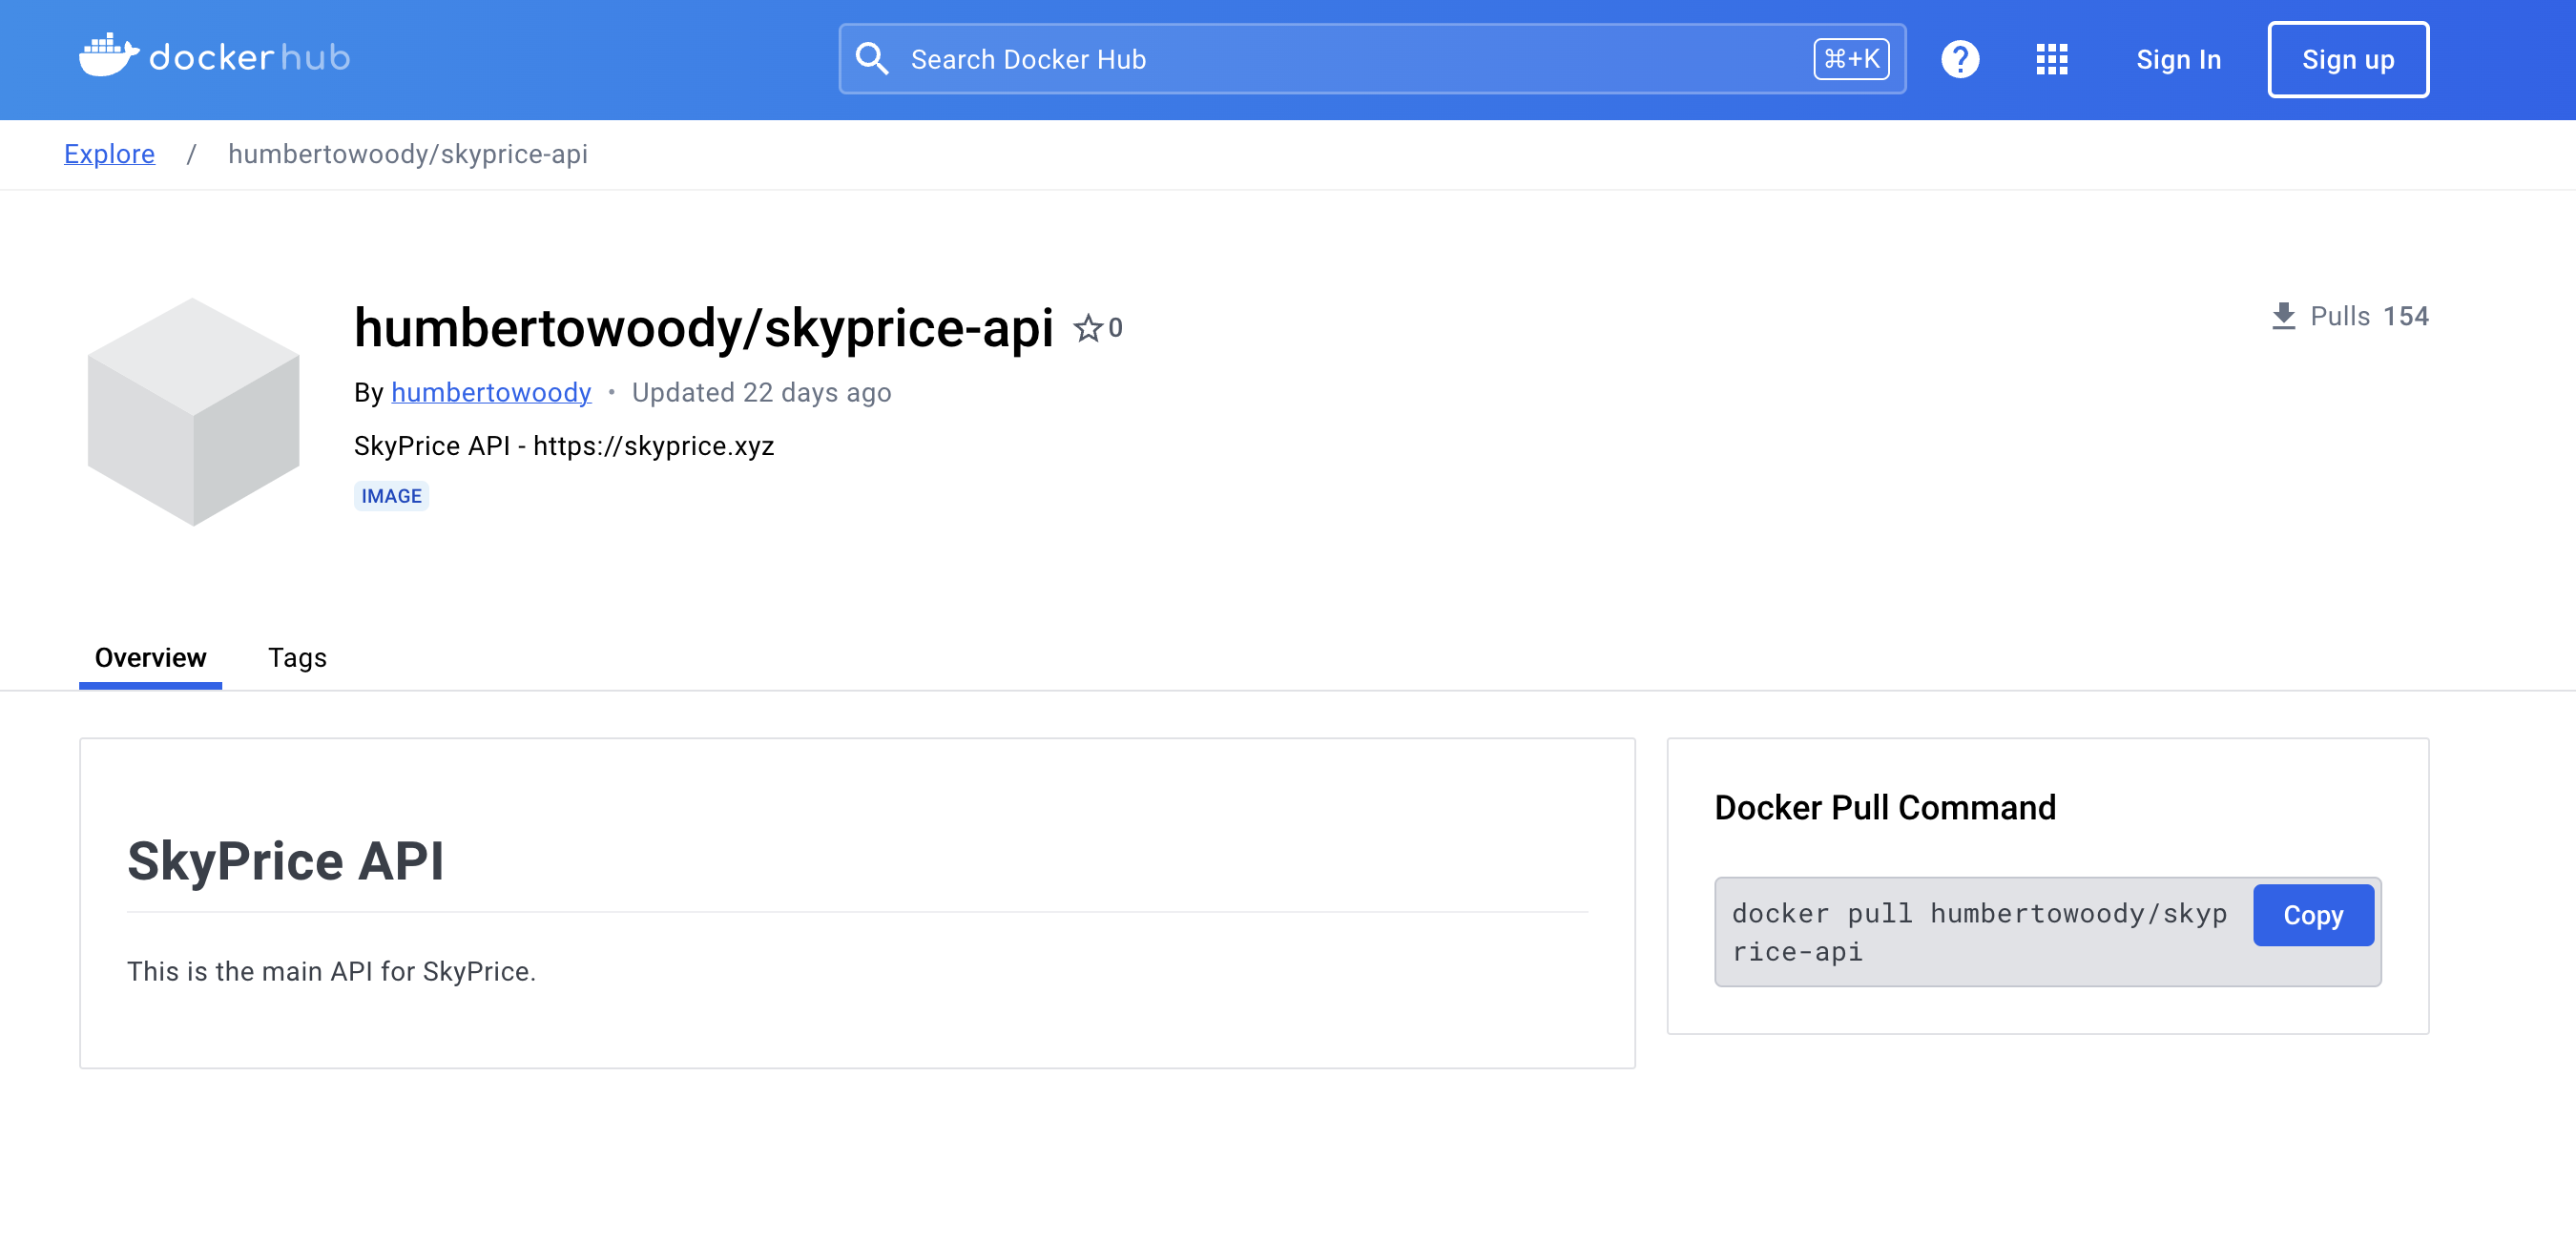
\includegraphics[width=0.8\textwidth]{imagenes/05-implementacion/despliegue/dockerhub.png}
    \caption{Imagen de Docker publicada en Docker Hub \cite{skypricedockerhub}.}
    \label{fig:docker-hub}
\end{figure}

\subsection{Despliegue del servicio web}
Una vez que el servicio web se encuentra en Docker Hub, se inicia su despliegue
en AWS utilizando Elastic Beanstalk. Para ello, primeramente se crea un nuevo
certificado SSL en AWS Certificate Manager, el cual se asocia al dominio de la
aplicación. Posteriormente, se crea un entorno de Elastic Beanstalk para la
aplicación, se configuran las variables de entorno y se despliega la imagen de
Docker en el entorno.

\subsubsection{AWS Certificate Manager}
Utilizar un certificado SSL es importante para garantizar la seguridad y la
confidencialidad de los datos que se transmiten entre el cliente y el servidor.
Más aún, en el caso de aplicaciones web, es fundamental para proteger la
información sensible de los usuarios, como contraseñas, datos personales y
financieros. Por ello, se creó un certificado SSL en AWS Certificate Manager
para el dominio de la aplicación, el cual se muestra en la figura
\ref{fig:certificado-ssl}. Este certificado SSL responde a dos subdominios:
\texttt{api.skyprice.xyz} y \texttt{skyprice.xyz}. El primero se utiliza para
el servicio web y el segundo para la interfaz gráfica, lo que permite garantizar
la integridad de ambas partes.

\begin{figure}[H]
    \centering
    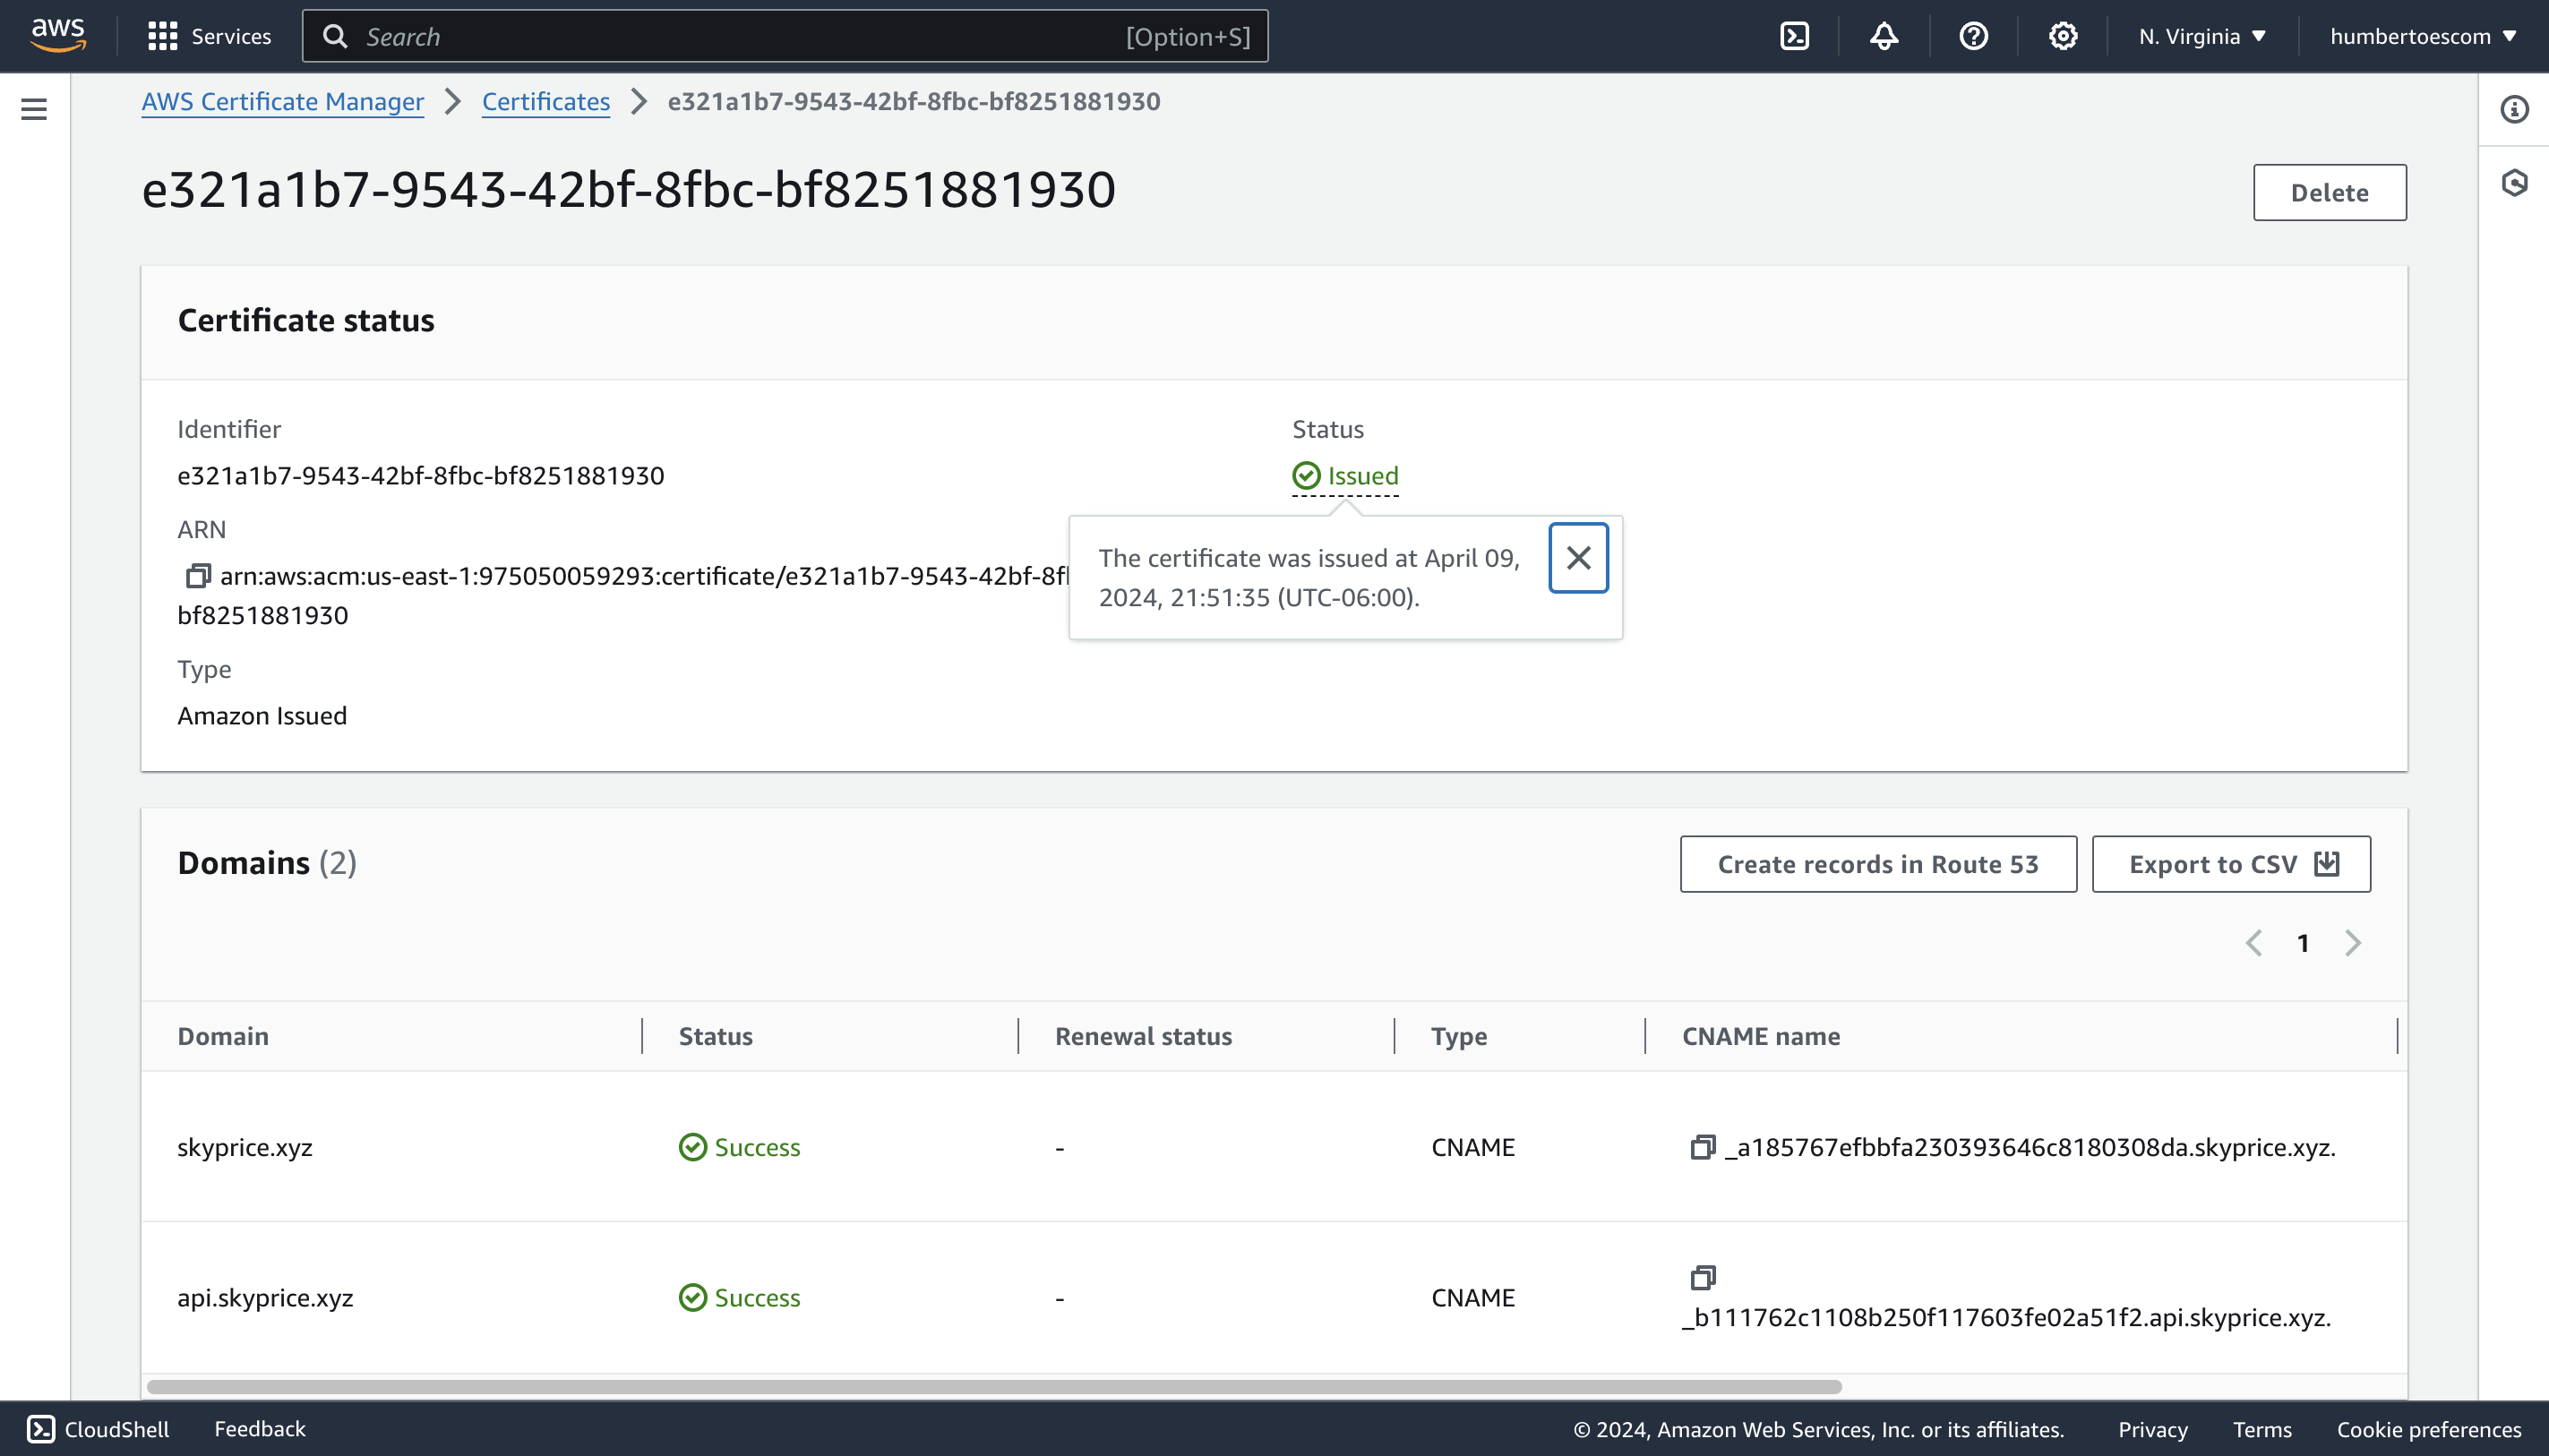
\includegraphics[width=0.8\textwidth]{imagenes/05-implementacion/despliegue/aws-certificate-manager.png}
    \caption{Certificado SSL en AWS Certificate Manager.}
    \label{fig:certificado-ssl}
\end{figure}

Aunado a esto, fue necesario configurar el dominio para que integrara los registros
requeridos para la validación del certificado SSL. En la figura \ref{fig:registros-dns}
se muestra la configuración de los registros DNS para el dominio de la aplicación.

\begin{figure}[H]
    \centering
    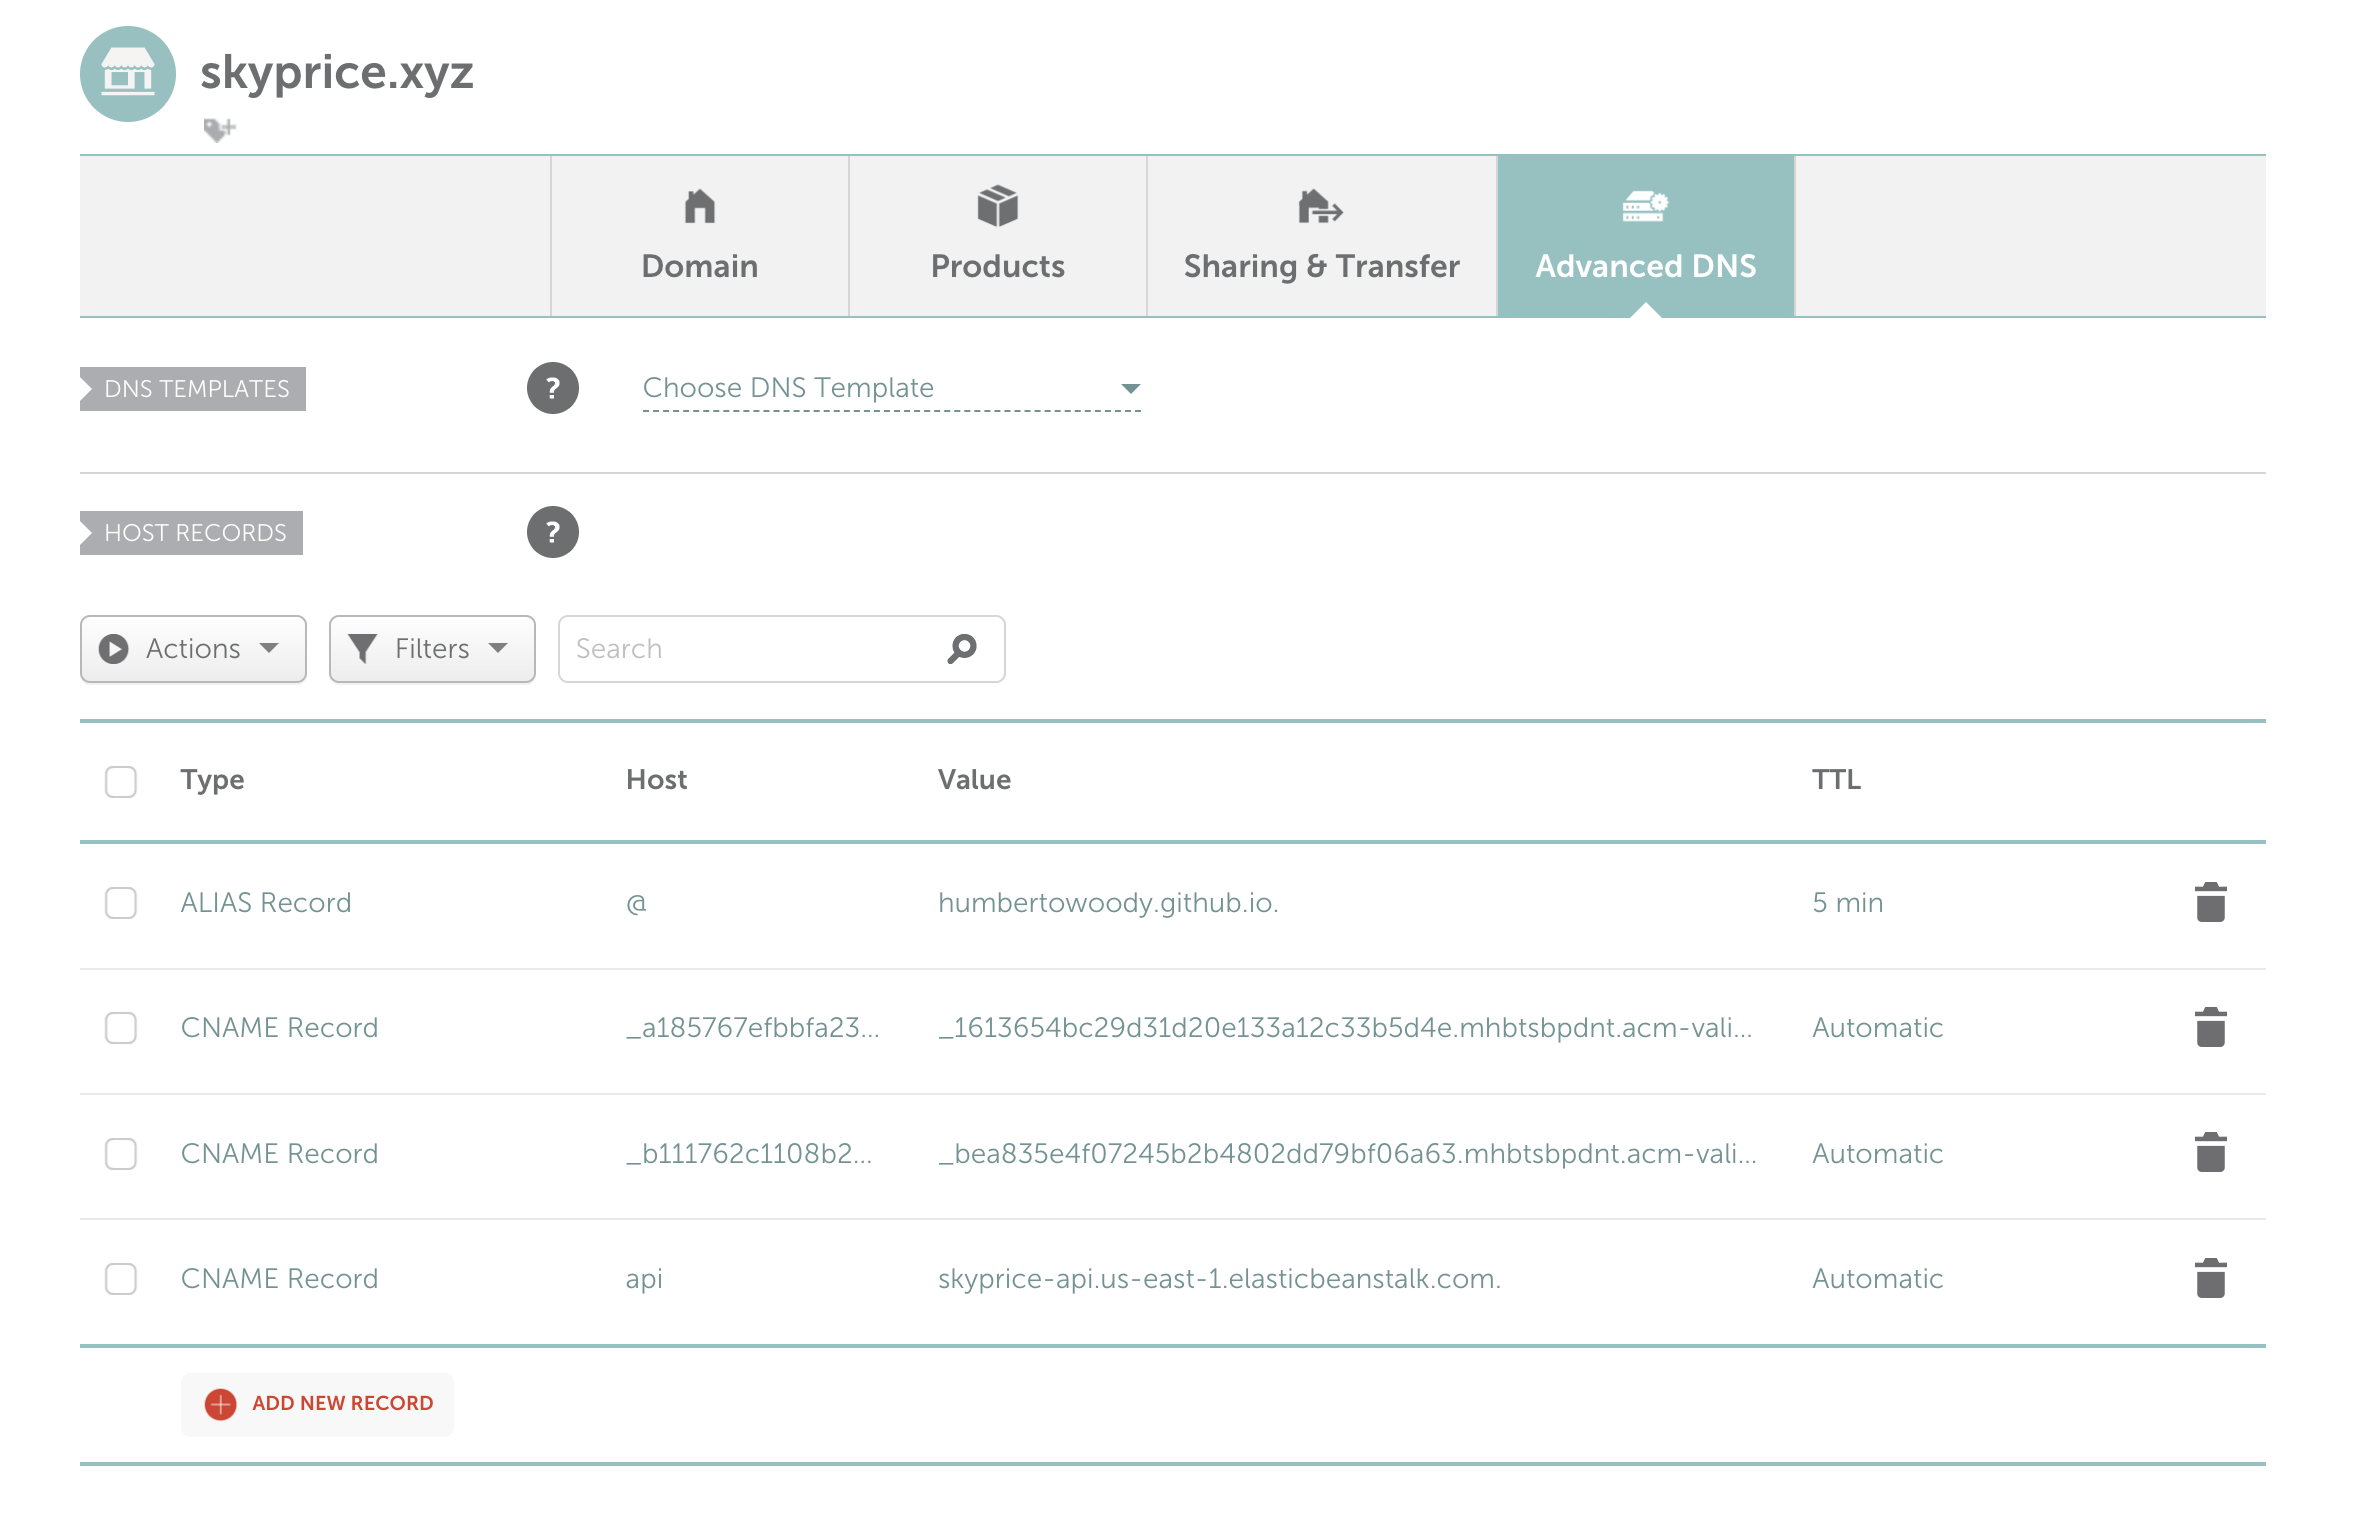
\includegraphics[width=0.8\textwidth]{imagenes/05-implementacion/despliegue/namecheapadvanceddns.png}
    \caption{Registros DNS para el dominio de la aplicación.}
    \label{fig:registros-dns}
\end{figure}

Una vez que AWS Certificate Manager validó el certificado SSL, ahora se puede
crear el entorno de Elastic Beanstalk para la aplicación y asociar el certificado
SSL al dominio de la aplicación, lo que garantiza una conexión segura y cifrada.

\subsubsection{AWS Elastic Beanstalk}
Elastic Beanstalk es un servicio de AWS que facilita el despliegue y la administración
de aplicaciones web y servicios en la nube. Usarlo requiere crear un ambiente,
el cual se llamará \texttt{skyprice-api} en este caso, y configurar las variables
de entorno necesarias para la aplicación. Cuando se crea un ambiente, debe seleccionarse
la plataforma de Docker, ya que la aplicación se ejecuta en un contenedor Docker,
y se debe especificar la imagen de Docker que se utilizará para el despliegue,
en nuestro caso, la imagen de Docker publicada en Docker Hub.

En el listado \ref{lst:elastic-beanstalk} se muestra el archivo de configuración
\texttt{Dockerrun.aws.json} que se utiliza para especificar la configuración del
contenedor Docker en Elastic Beanstalk. En este archivo se define la imagen de Docker
que se utilizará, así como la configuración de red que se aplicará al contenedor.
Es importante destacar que se está utilizando la versión 1 de \texttt{AWSEBDockerrunVersion}
ya que es la versión adecuada para un único contenedor Docker, la versión 2 se utiliza
para aplicaciones multicontenedor.

\begin{lstlisting}[language=json, caption={Archivo de configuración para Elastic Beanstalk}, label={lst:elastic-beanstalk}]
{
  "AWSEBDockerrunVersion": "1",
  "Image": {
    "Name": "humbertowoody/skyprice-api:latest",
    "Update": "true"
  },
  "Ports": [{ "ContainerPort": 5000 }]
}
\end{lstlisting}

Una vez que se ha creado el ambiente y se ha configurado la imagen de Docker, se
puede desplegar la aplicación en Elastic Beanstalk. En la figura \ref{fig:elastic-beanstalk}
se muestra el panel de control de Elastic Beanstalk con el entorno de la aplicación
\texttt{skyprice-api} en ejecución.

\begin{figure}[H]
    \centering
    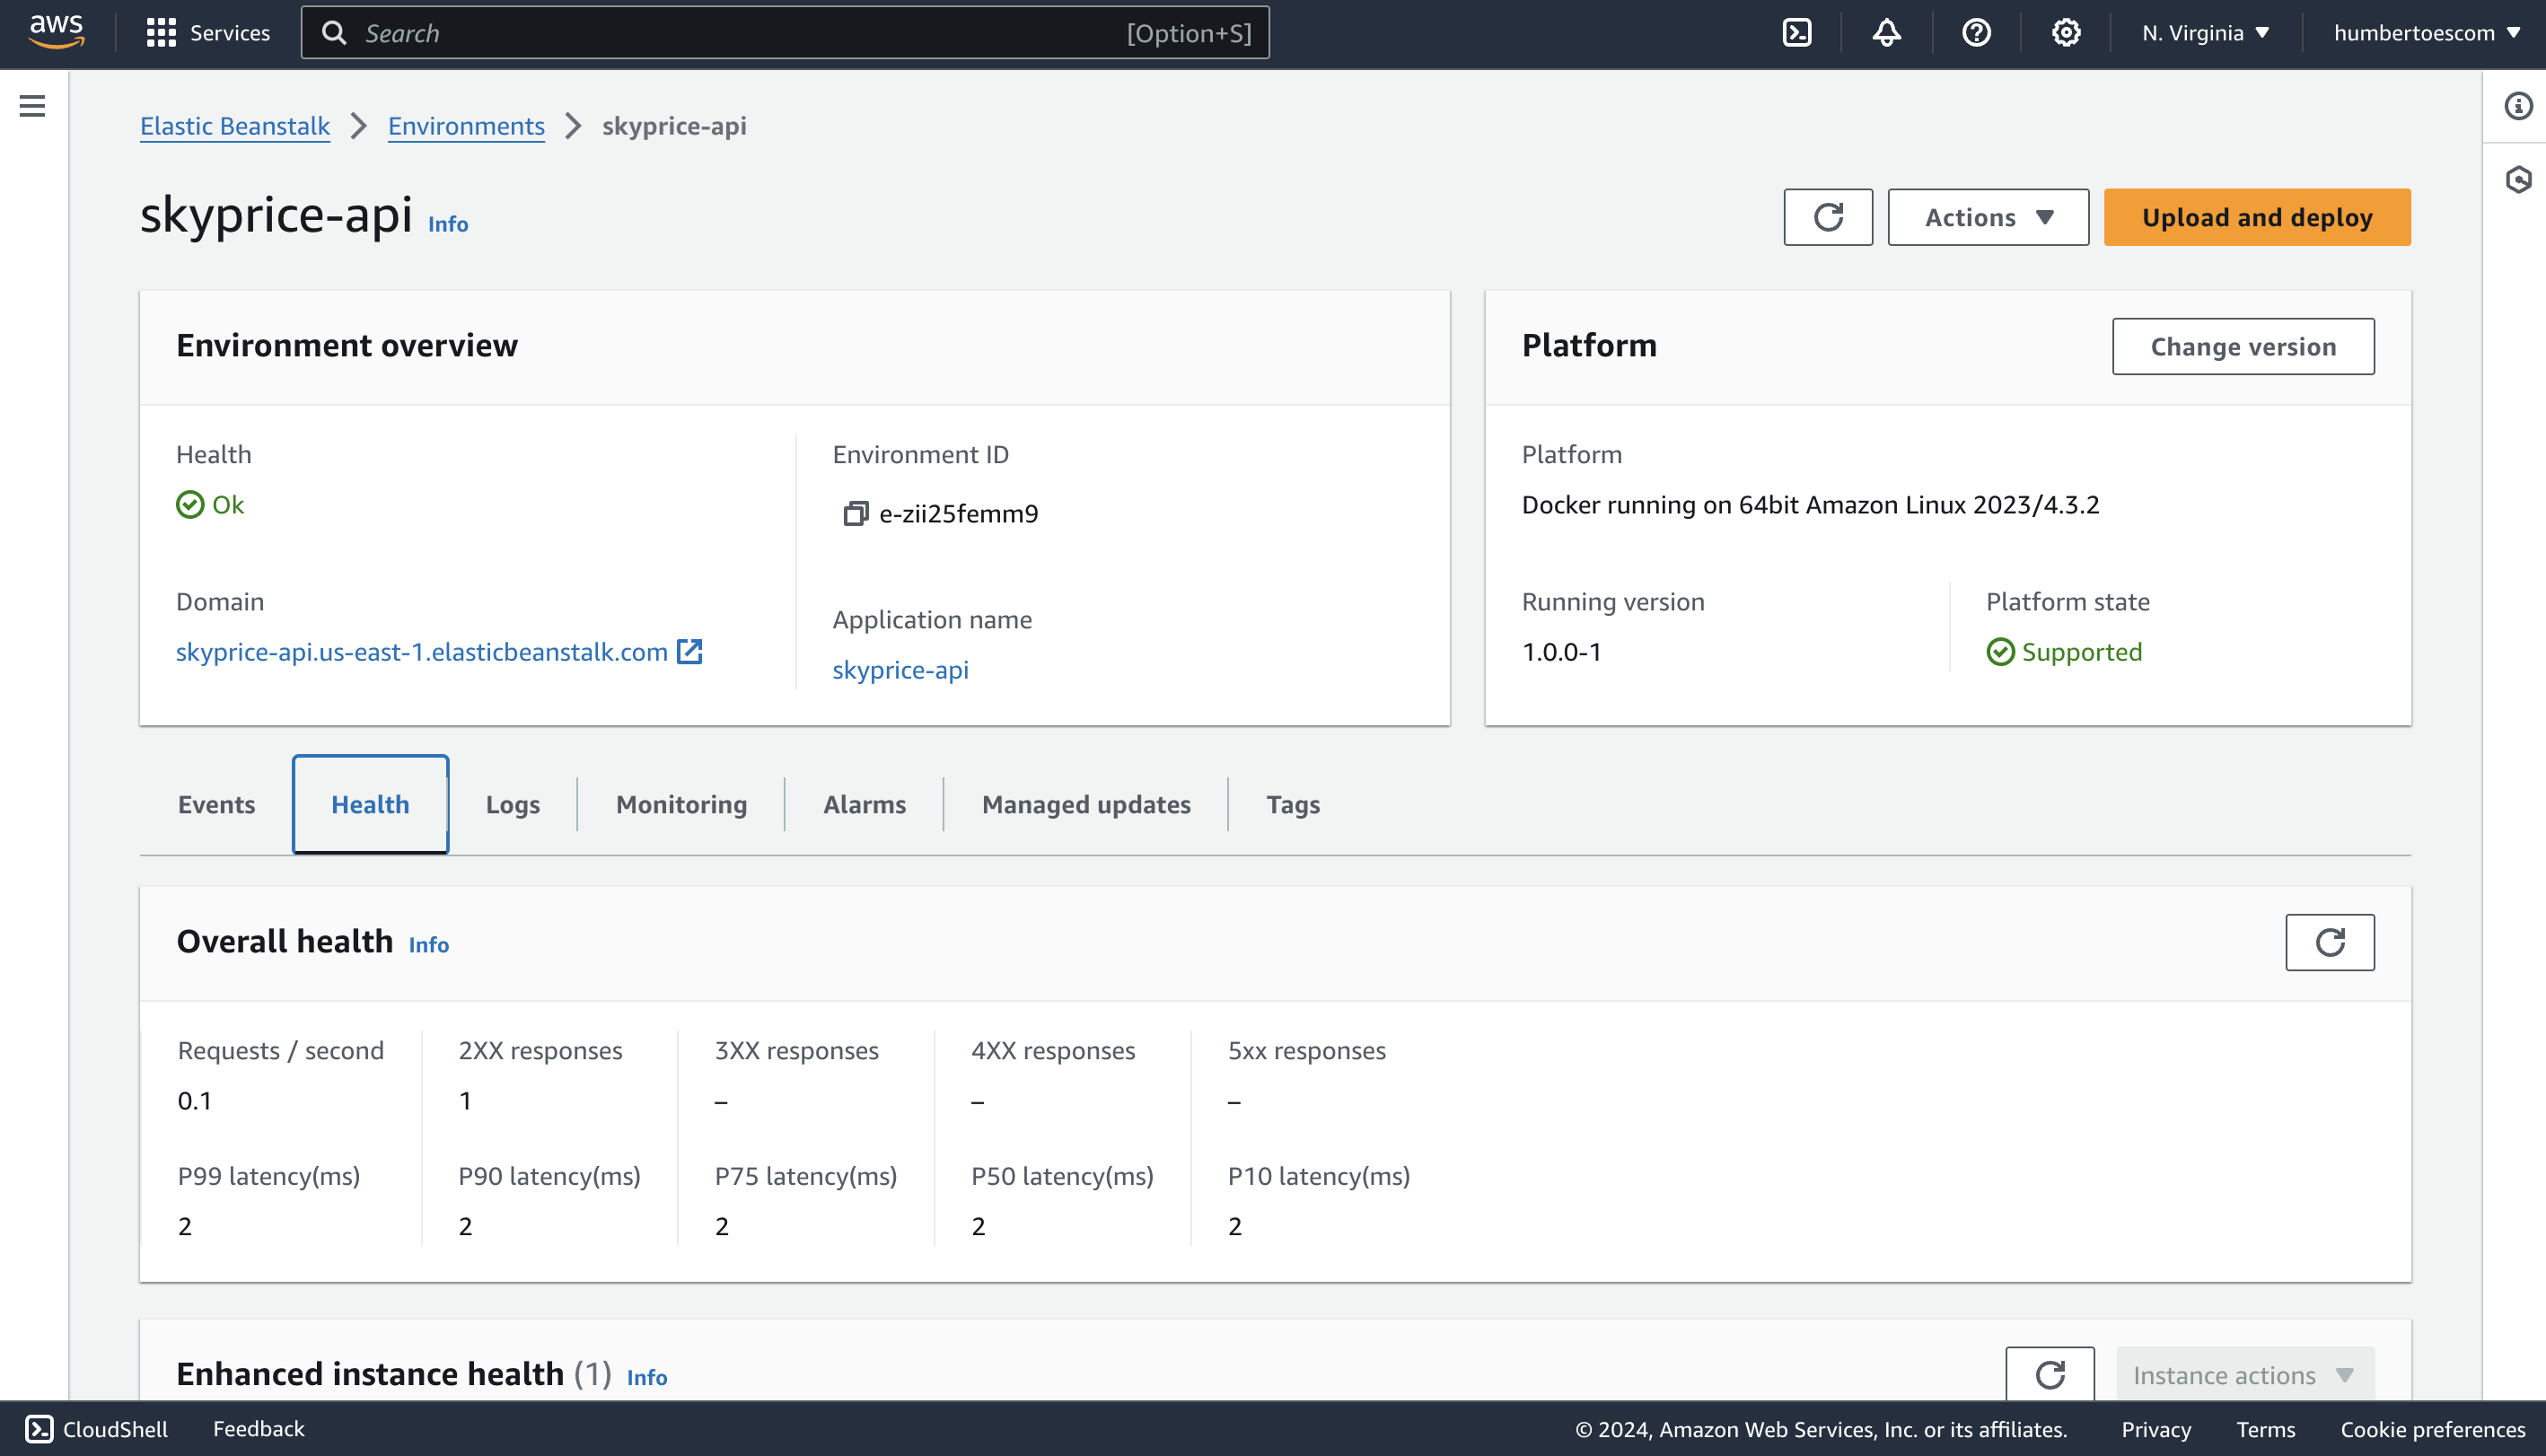
\includegraphics[width=1.0\textwidth]{imagenes/05-implementacion/despliegue/eb-skyprice-api-main.png}
    \caption{Entorno de Elastic Beanstalk en ejecución.}
    \label{fig:elastic-beanstalk}
\end{figure}

\subsubsection{Verificación del despliegue}
Una vez que la aplicación se ha desplegado en Elastic Beanstalk, es importante
verificar que el despliegue se haya realizado correctamente y que la aplicación
esté funcionando correctamente. Para ello, se puede acceder a la URL proporcionada
por Elastic Beanstalk y verificar que la aplicación responda correctamente. Además,
se puede verificar que también se respondan a peticiones al dominio personalizado y
que el certificado SSL esté funcionando correctamente. En la figura \ref{fig:api-skyprice-xyz}
se muestra la respuesta de la aplicación al acceder a la URL \texttt{https://api.skyprice.xyz},
así como información del certificado SSL.

\begin{figure}[H]
    \centering
    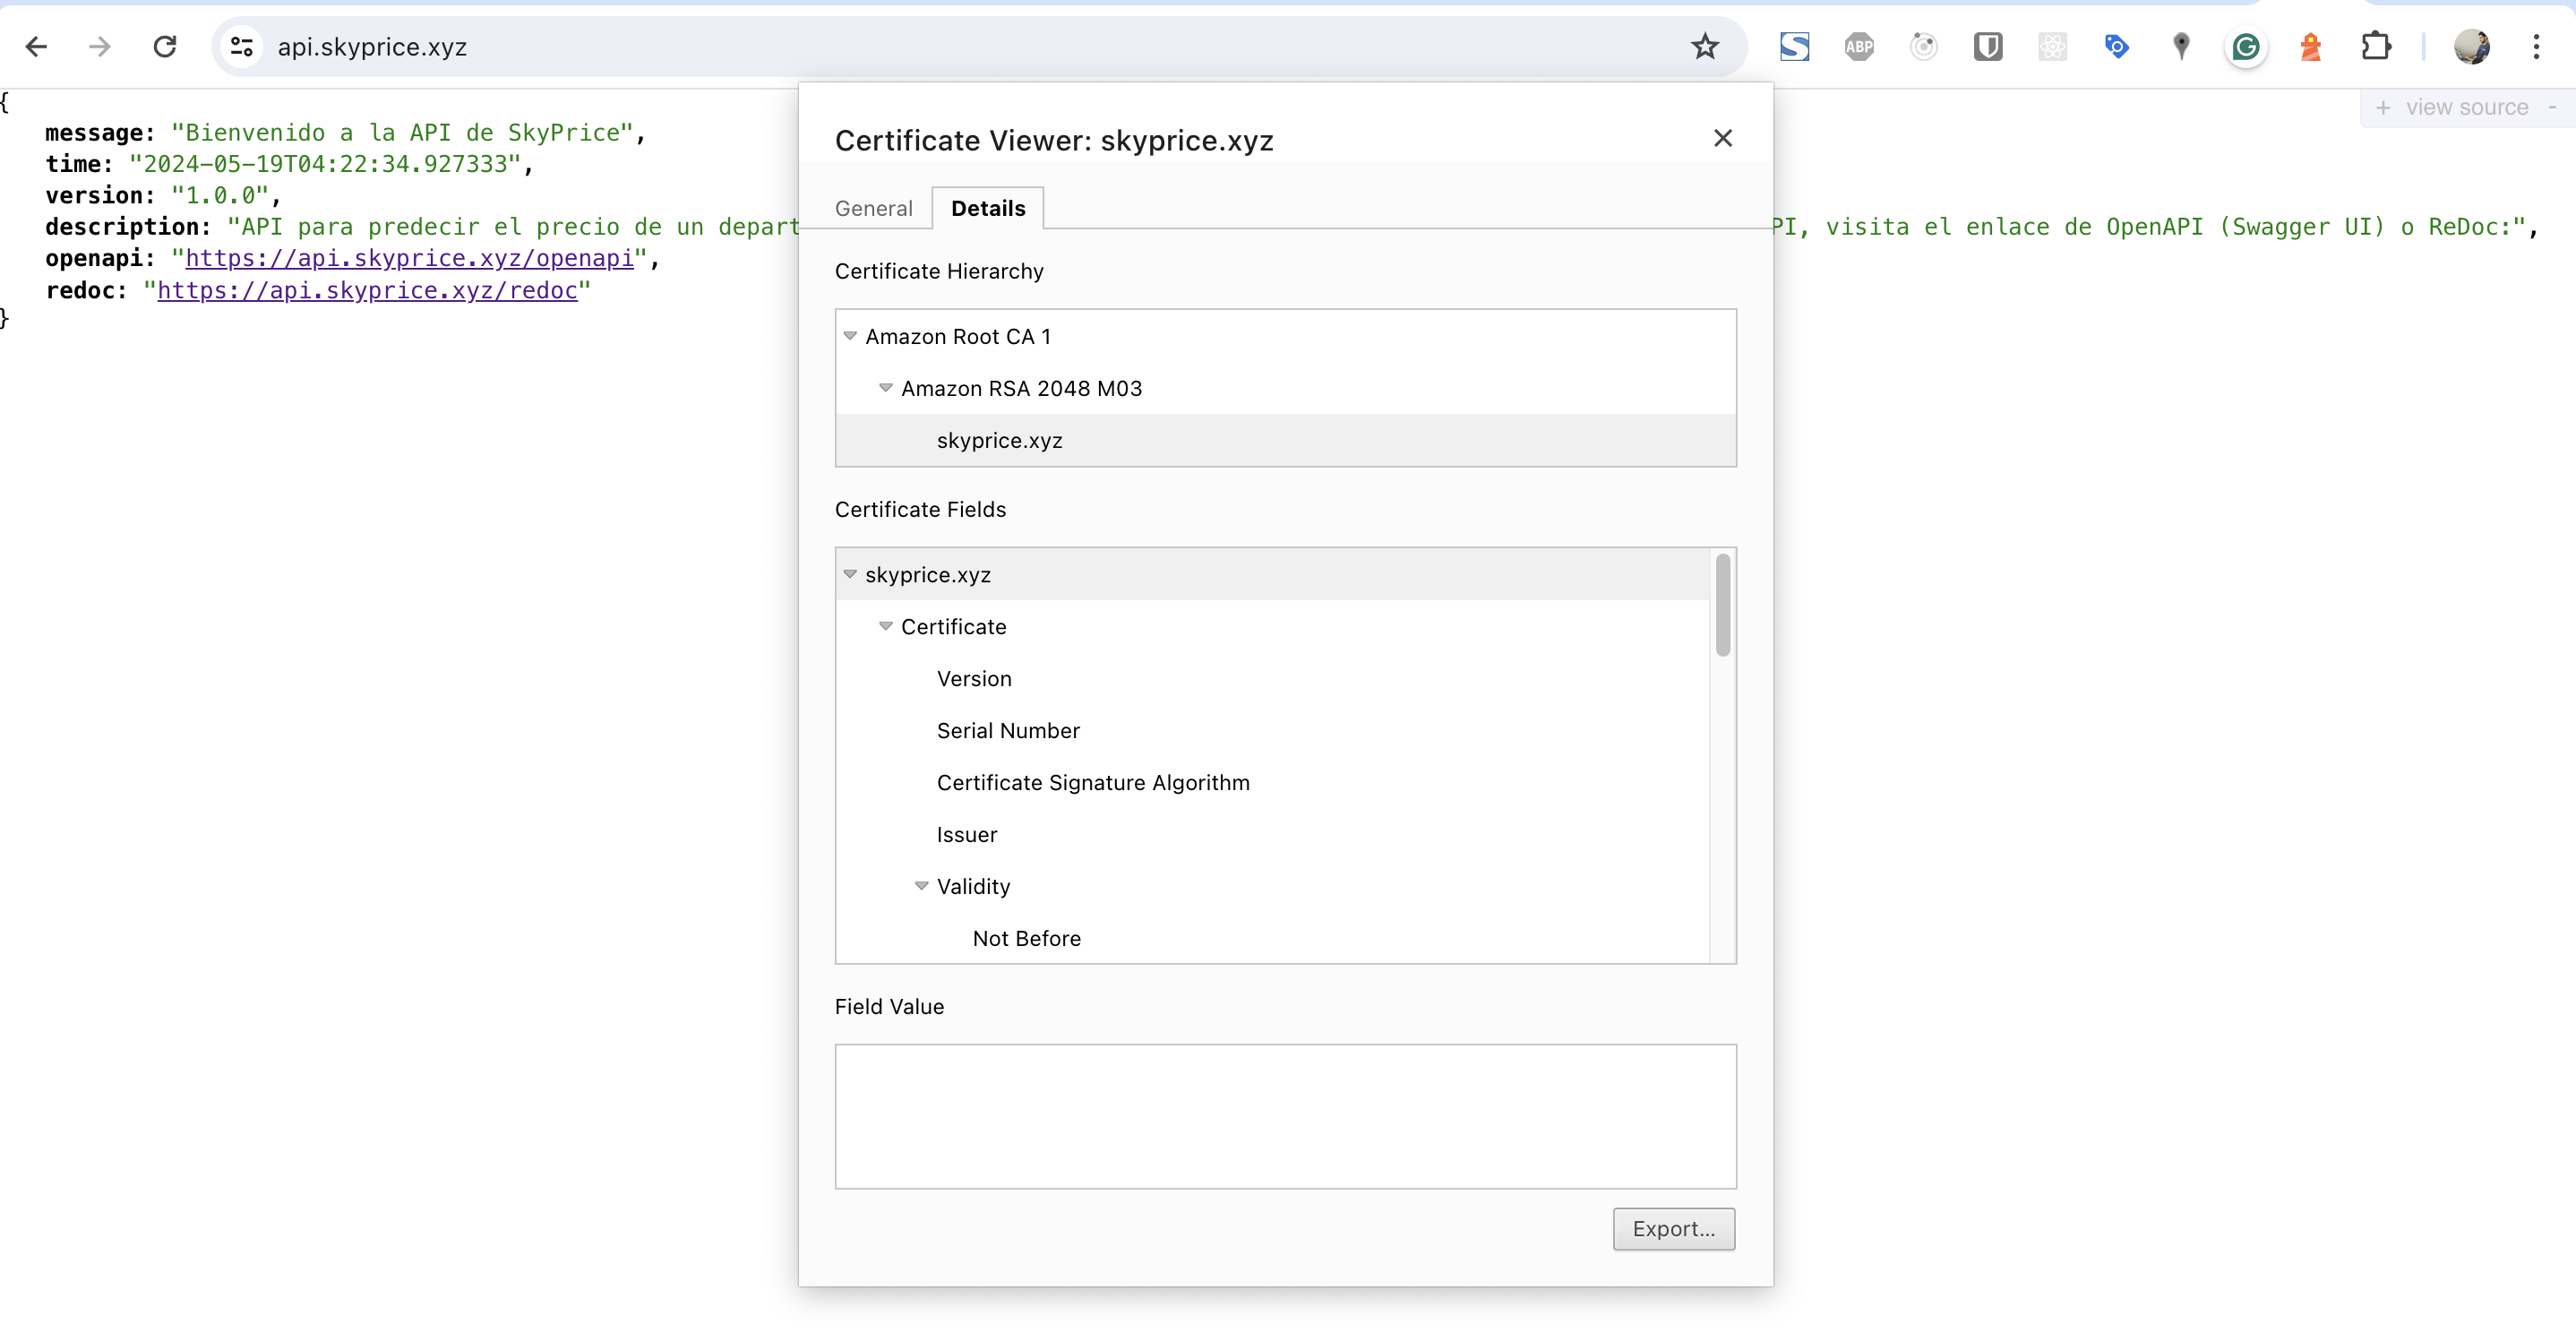
\includegraphics[width=1.0\textwidth]{imagenes/05-implementacion/despliegue/eb-ssl.png}
    \caption{Verificación SSL para la URL \texttt{https://api.skyprice.xyz}.}
    \label{fig:api-skyprice-xyz}
\end{figure}

\subsection{Despliegue de la interfaz gráfica}
La interfaz gráfica corresponde a una aplicación React utilizando NextJS, la cual
se construyó, minificó y empaquetó para su despliegue en un bucket de AWS S3. Posteriormente
se configuró un CDN con AWS CloudFront para distribuir el contenido de manera eficiente y segura.

\subsubsection{Compilación y empaquetado}
Para compilar y empaquetar la interfaz gráfica, se utilizó el comando \texttt{npm build}
de NextJS, el cual compila la aplicación y la empaqueta en una carpeta \texttt{out}
que contiene los archivos estáticos y optimizados para producción. Posteriormente,
estos archivos serán subidos a un bucket de AWS S3 para su distribución.

En la figura \ref{fig:next-build} se muestra la salida del comando \texttt{npm build}
en la terminal, donde se puede observar que la compilación se realizó correctamente y
que se generaron los archivos estáticos en la carpeta \texttt{out}.

\begin{figure}[H]
    \centering
    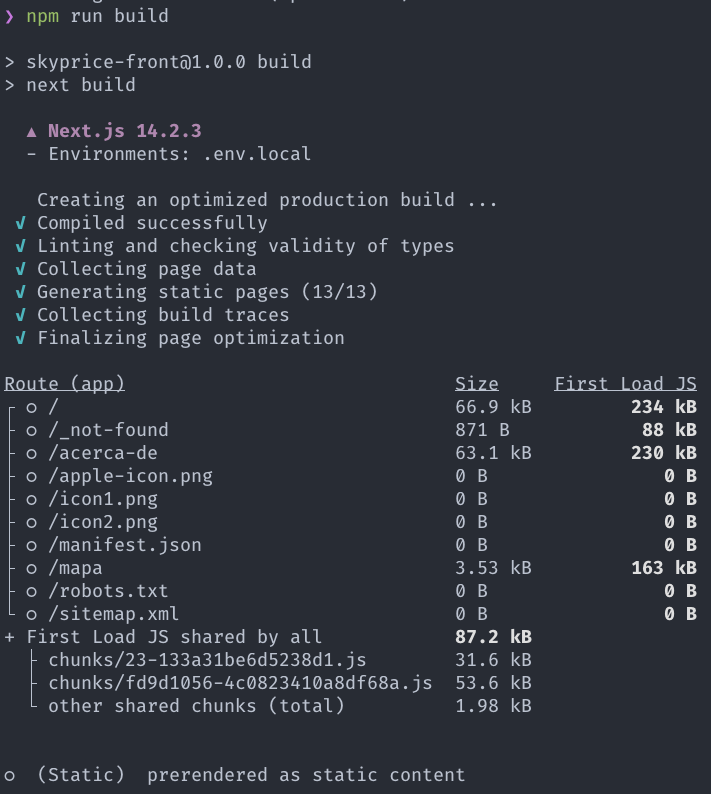
\includegraphics[width=1.0\textwidth]{imagenes/05-implementacion/despliegue/npm-build.png}
    \caption{Compilación de la interfaz gráfica con NextJS.}
    \label{fig:next-build}
\end{figure}

\subsubsection{AWS S3}
La interfaz gráfica se desplegó en un bucket de AWS S3, lo que permite servir los
archivos estáticos de manera eficiente y segura. Se configuró el bucket para ser
accesible públicamente y se implementaron políticas de seguridad adecuadas. En
la figura \ref{fig:aws-s3} se muestra el panel de control de AWS S3 con el bucket
\texttt{skyprice-front} en el que se alojó la interfaz gráfica.

\begin{figure}[H]
    \centering
    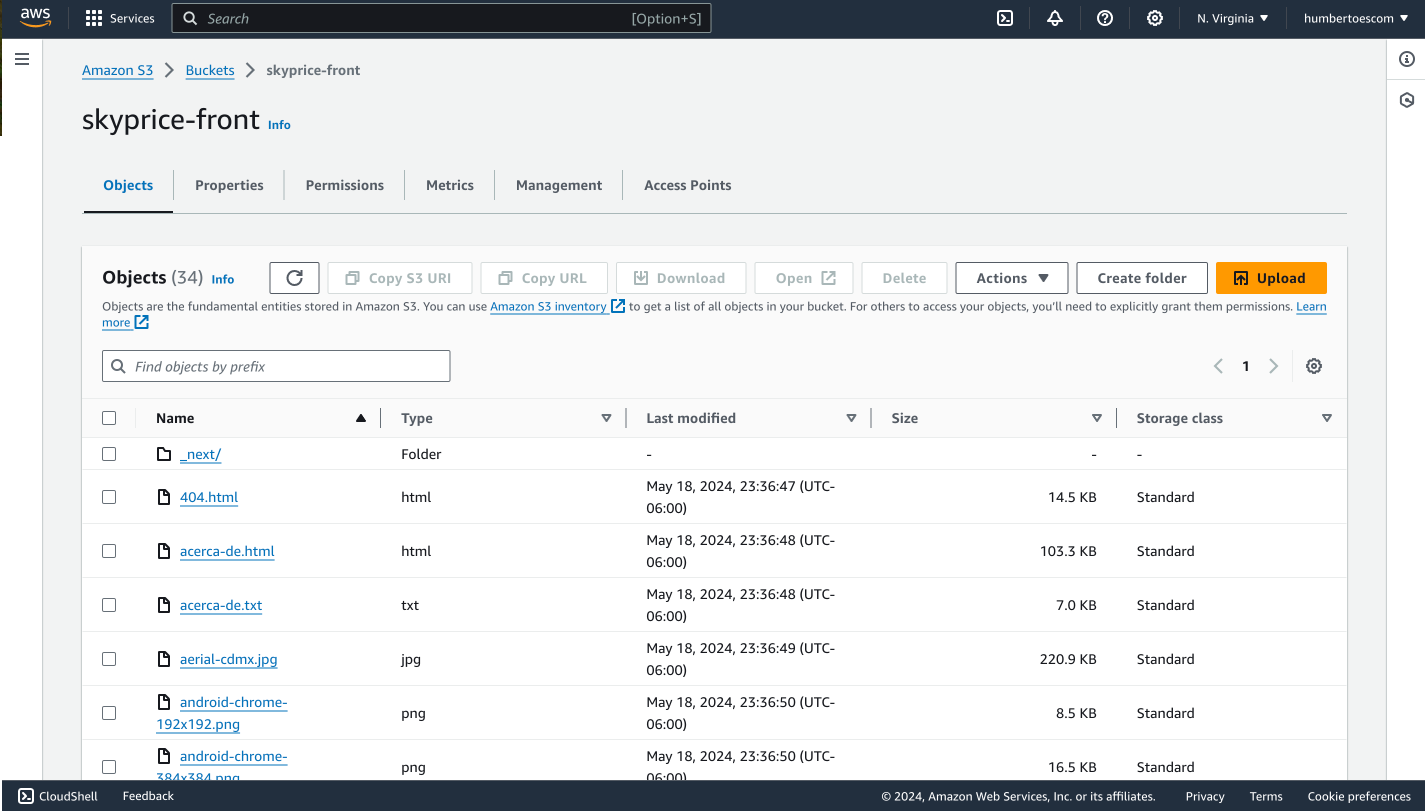
\includegraphics[width=1.0\textwidth]{imagenes/05-implementacion/despliegue/aws-s3.png}
    \caption{Bucket de AWS S3 con la interfaz gráfica.}
    \label{fig:aws-s3}
\end{figure}

\subsubsection{AWS CloudFront}
Se utilizó AWS CloudFront para distribuir el contenido de la interfaz gráfica a
través de una red de distribución de contenido (CDN). Esto mejora el rendimiento
y reduce la latencia para los usuarios de diferentes regiones geográficas. Además,
CloudFront proporciona una capa adicional de seguridad y protección contra ataques
Distributed Denial of Service (DDoS) \cite{aws_cloudfront_intro}.

En la figura \ref{fig:cloudfront} se muestra el panel de control de AWS CloudFront
con la distribución de contenido creada para la interfaz gráfica. Se configuró
CloudFront para que se conecte al bucket de S3 y distribuya el contenido de manera
eficiente y segura.

\begin{figure}[H]
    \centering
    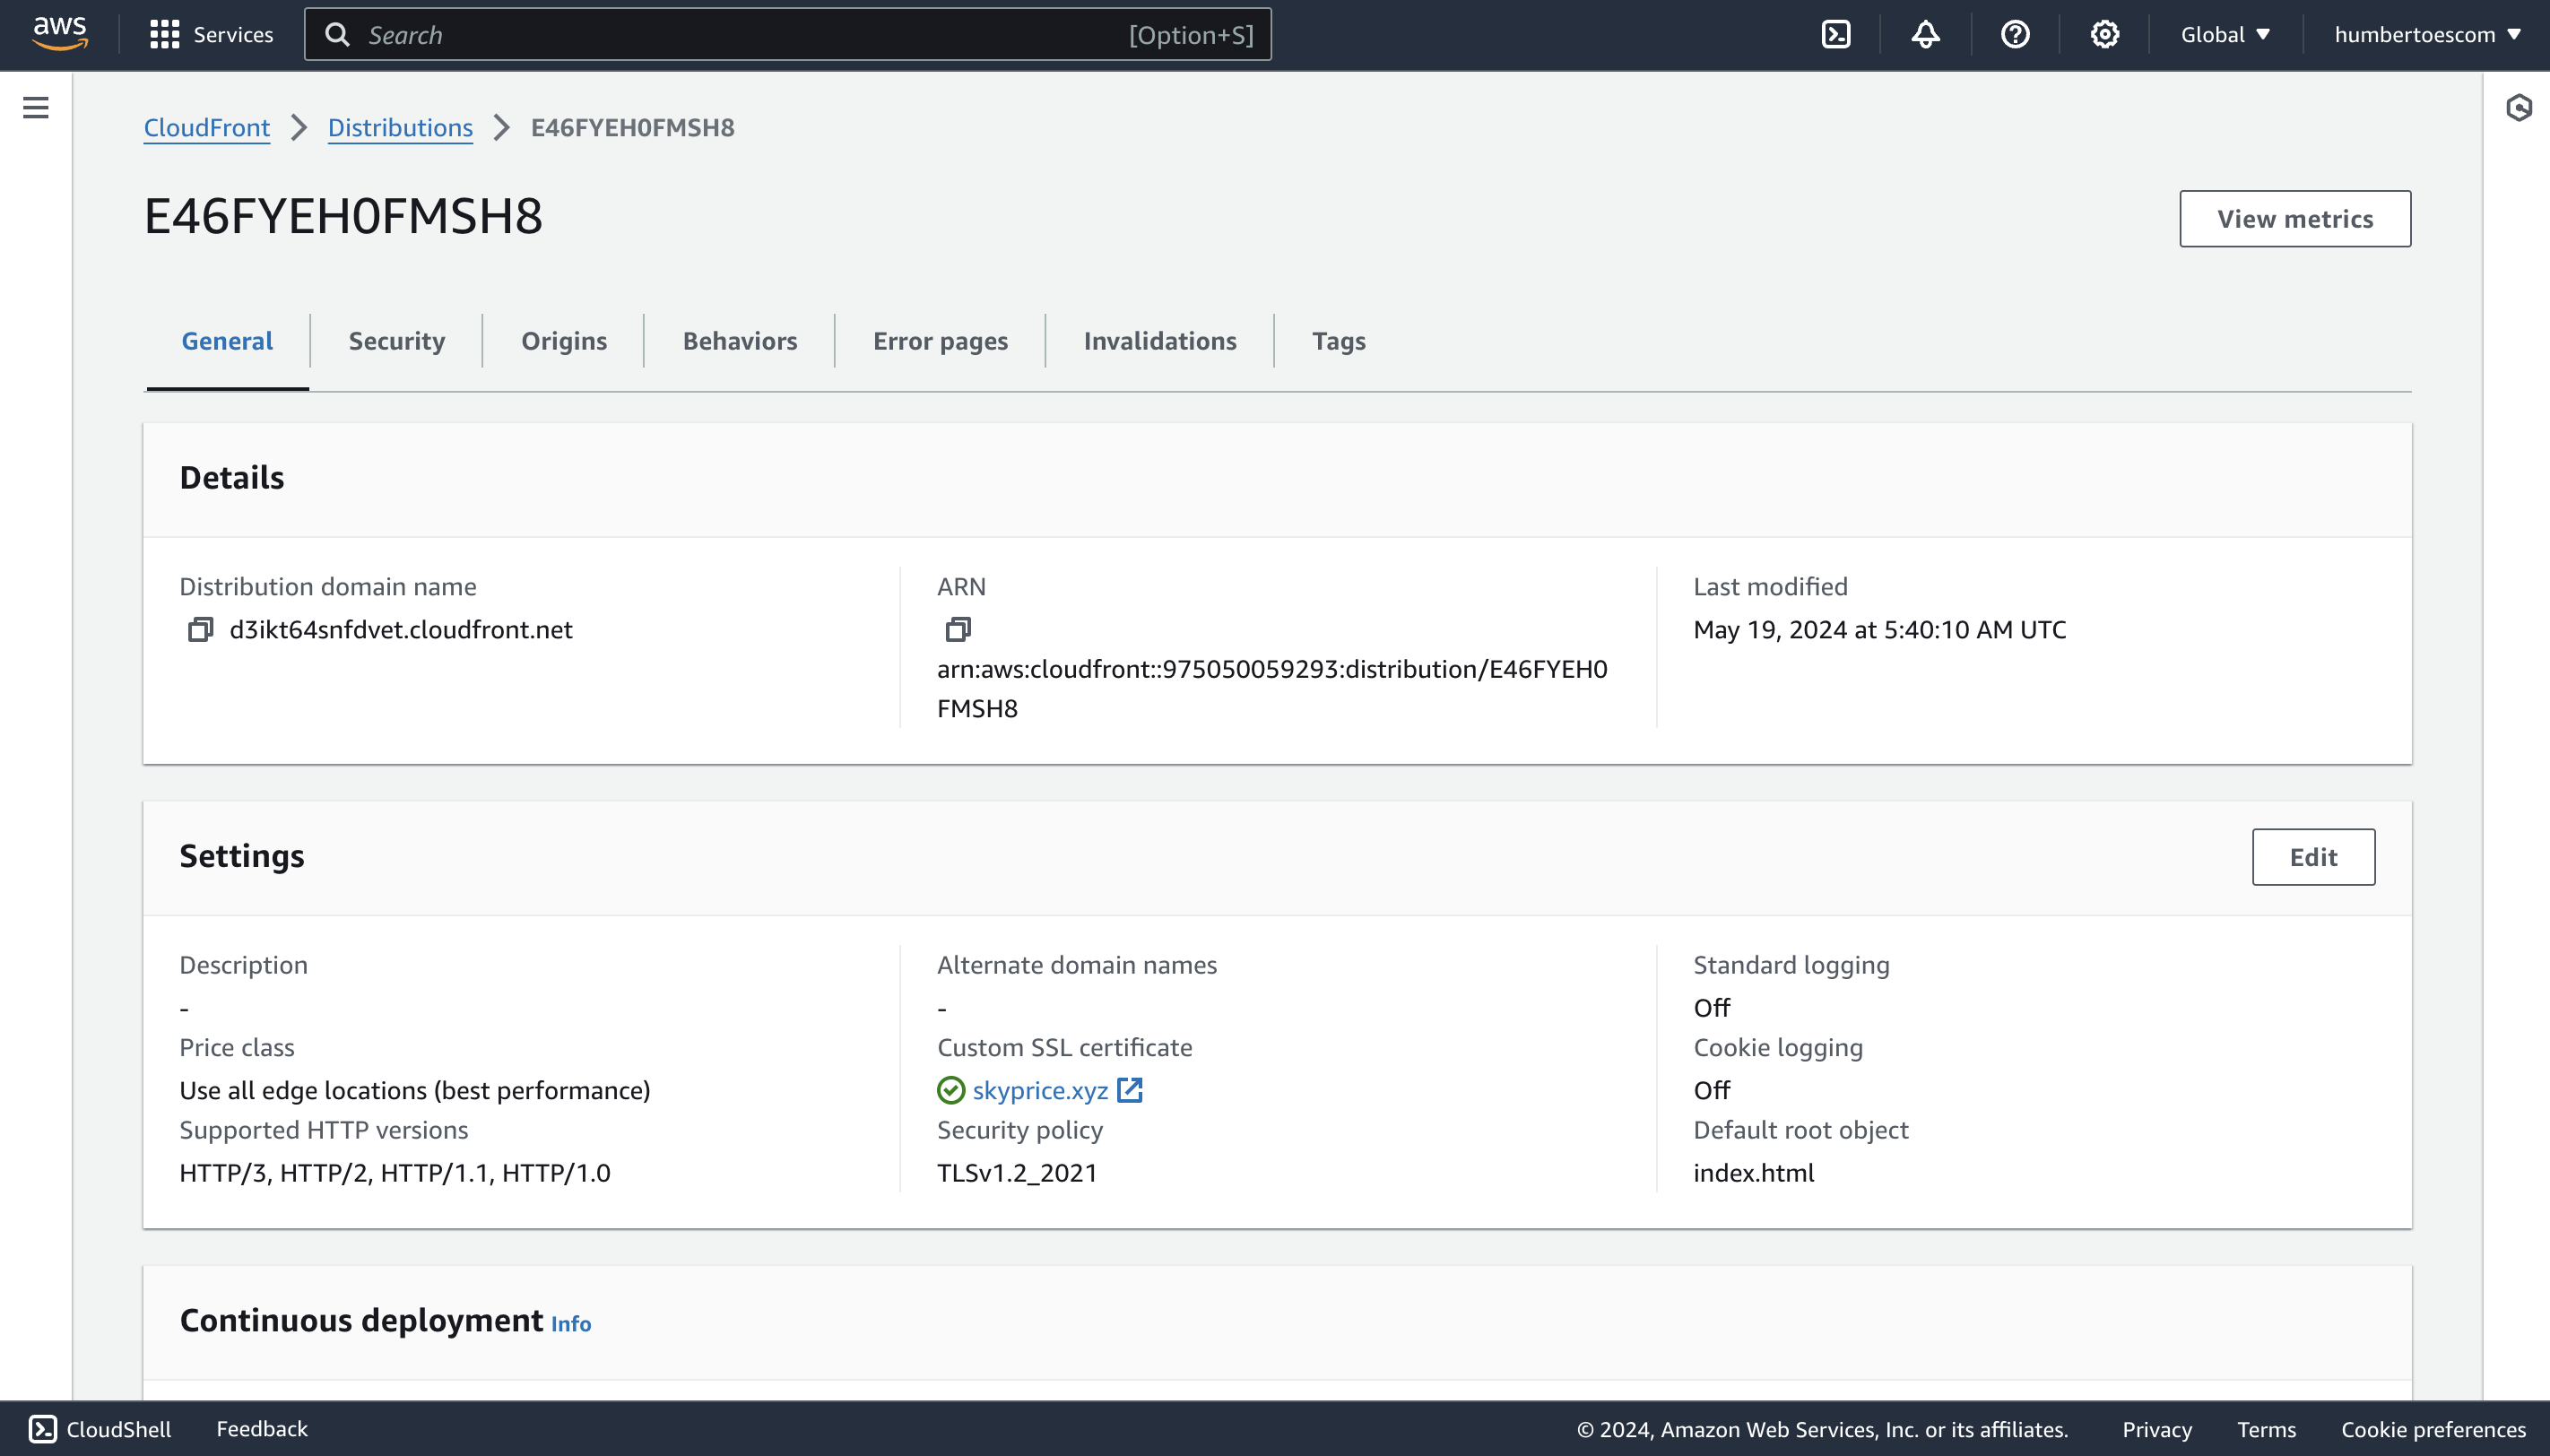
\includegraphics[width=1.0\textwidth]{imagenes/05-implementacion/despliegue/aws-cloudfront.png}
    \caption{Distribución de contenido de AWS CloudFront.}
    \label{fig:cloudfront}
\end{figure}

\subsubsection{Verificación del despliegue}
Una vez que la interfaz gráfica se ha desplegado en AWS S3 y se ha configurado
CloudFront para distribuir el contenido, es importante verificar que el despliegue
se haya realizado correctamente y que la aplicación esté funcionando correctamente.
Para ello, se puede acceder a la URL proporcionada por CloudFront y verificar que
la aplicación responda correctamente. En la figura \ref{fig:skyprice-xyz-front} se
muestra la respuesta de la aplicación al acceder a la URL \texttt{https://skyprice.xyz}.

\begin{figure}[H]
    \centering
    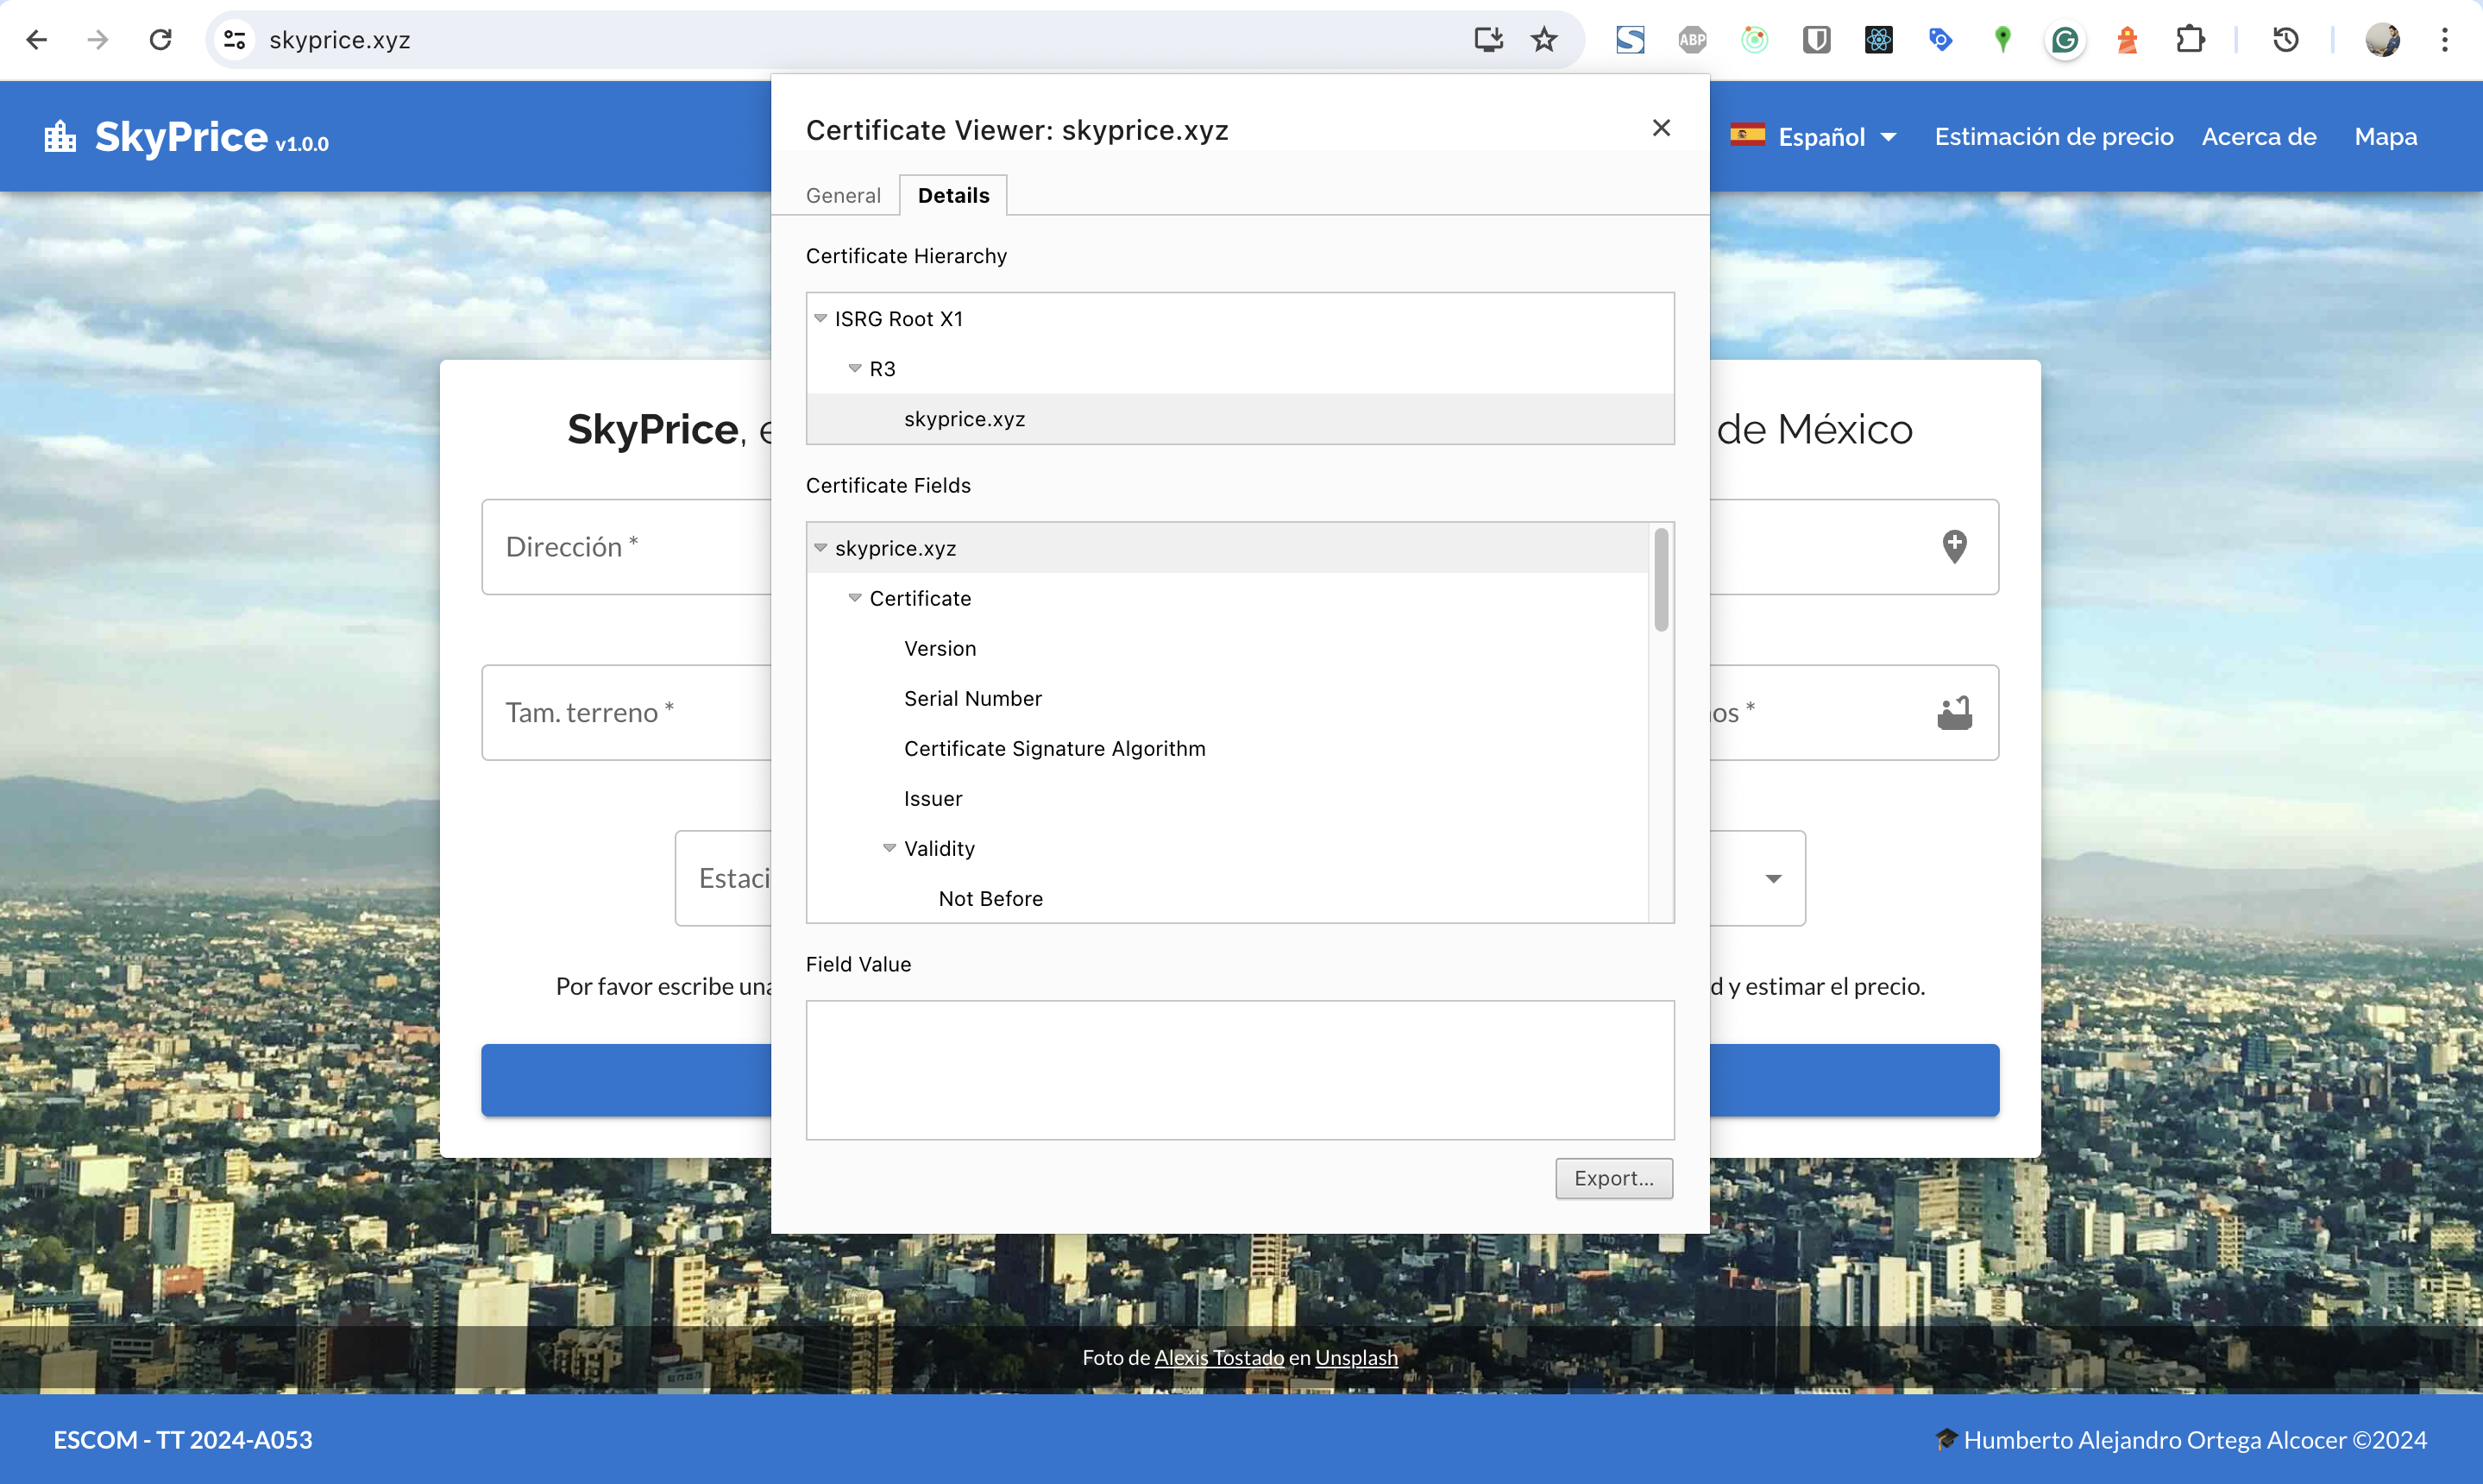
\includegraphics[width=1.0\textwidth]{imagenes/05-implementacion/despliegue/cloudfront-ssl.png}
    \caption{Verificación SSL para la URL \texttt{https://skyprice.xyz}.}
    \label{fig:skyprice-xyz-front}
\end{figure}

\subsection{Servicios externos}
Para el correcto funcionamiento de la aplicación, se utilizaron servicios externos
como Google Maps y ExchangeRate-API. Estos servicios permiten realizar la geocodificación
de direcciones y la conversión de monedas, respectivamente, lo que enriquece la
experiencia del usuario y agrega valor a la aplicación. En esta sección se describen
los servicios externos utilizados y se muestran ejemplos de su integración en la aplicación.

\subsubsection{Google Maps}
Para llevar a cabo la geocodificación de la dirección de la propiedad a estimar
su precio, se utilizó la API de \textit{Places} de Google Maps. Esta API permite
realizar búsquedas de direcciones y obtener información detallada sobre las mismas,
como coordenadas geográficas, nombres de lugares, tipos de establecimientos, entre
otros. En la figura \ref{fig:google-maps-api} se muestra la configuración de la
API de Google Maps en la consola de Google Cloud.

\begin{figure}[H]
    \centering
    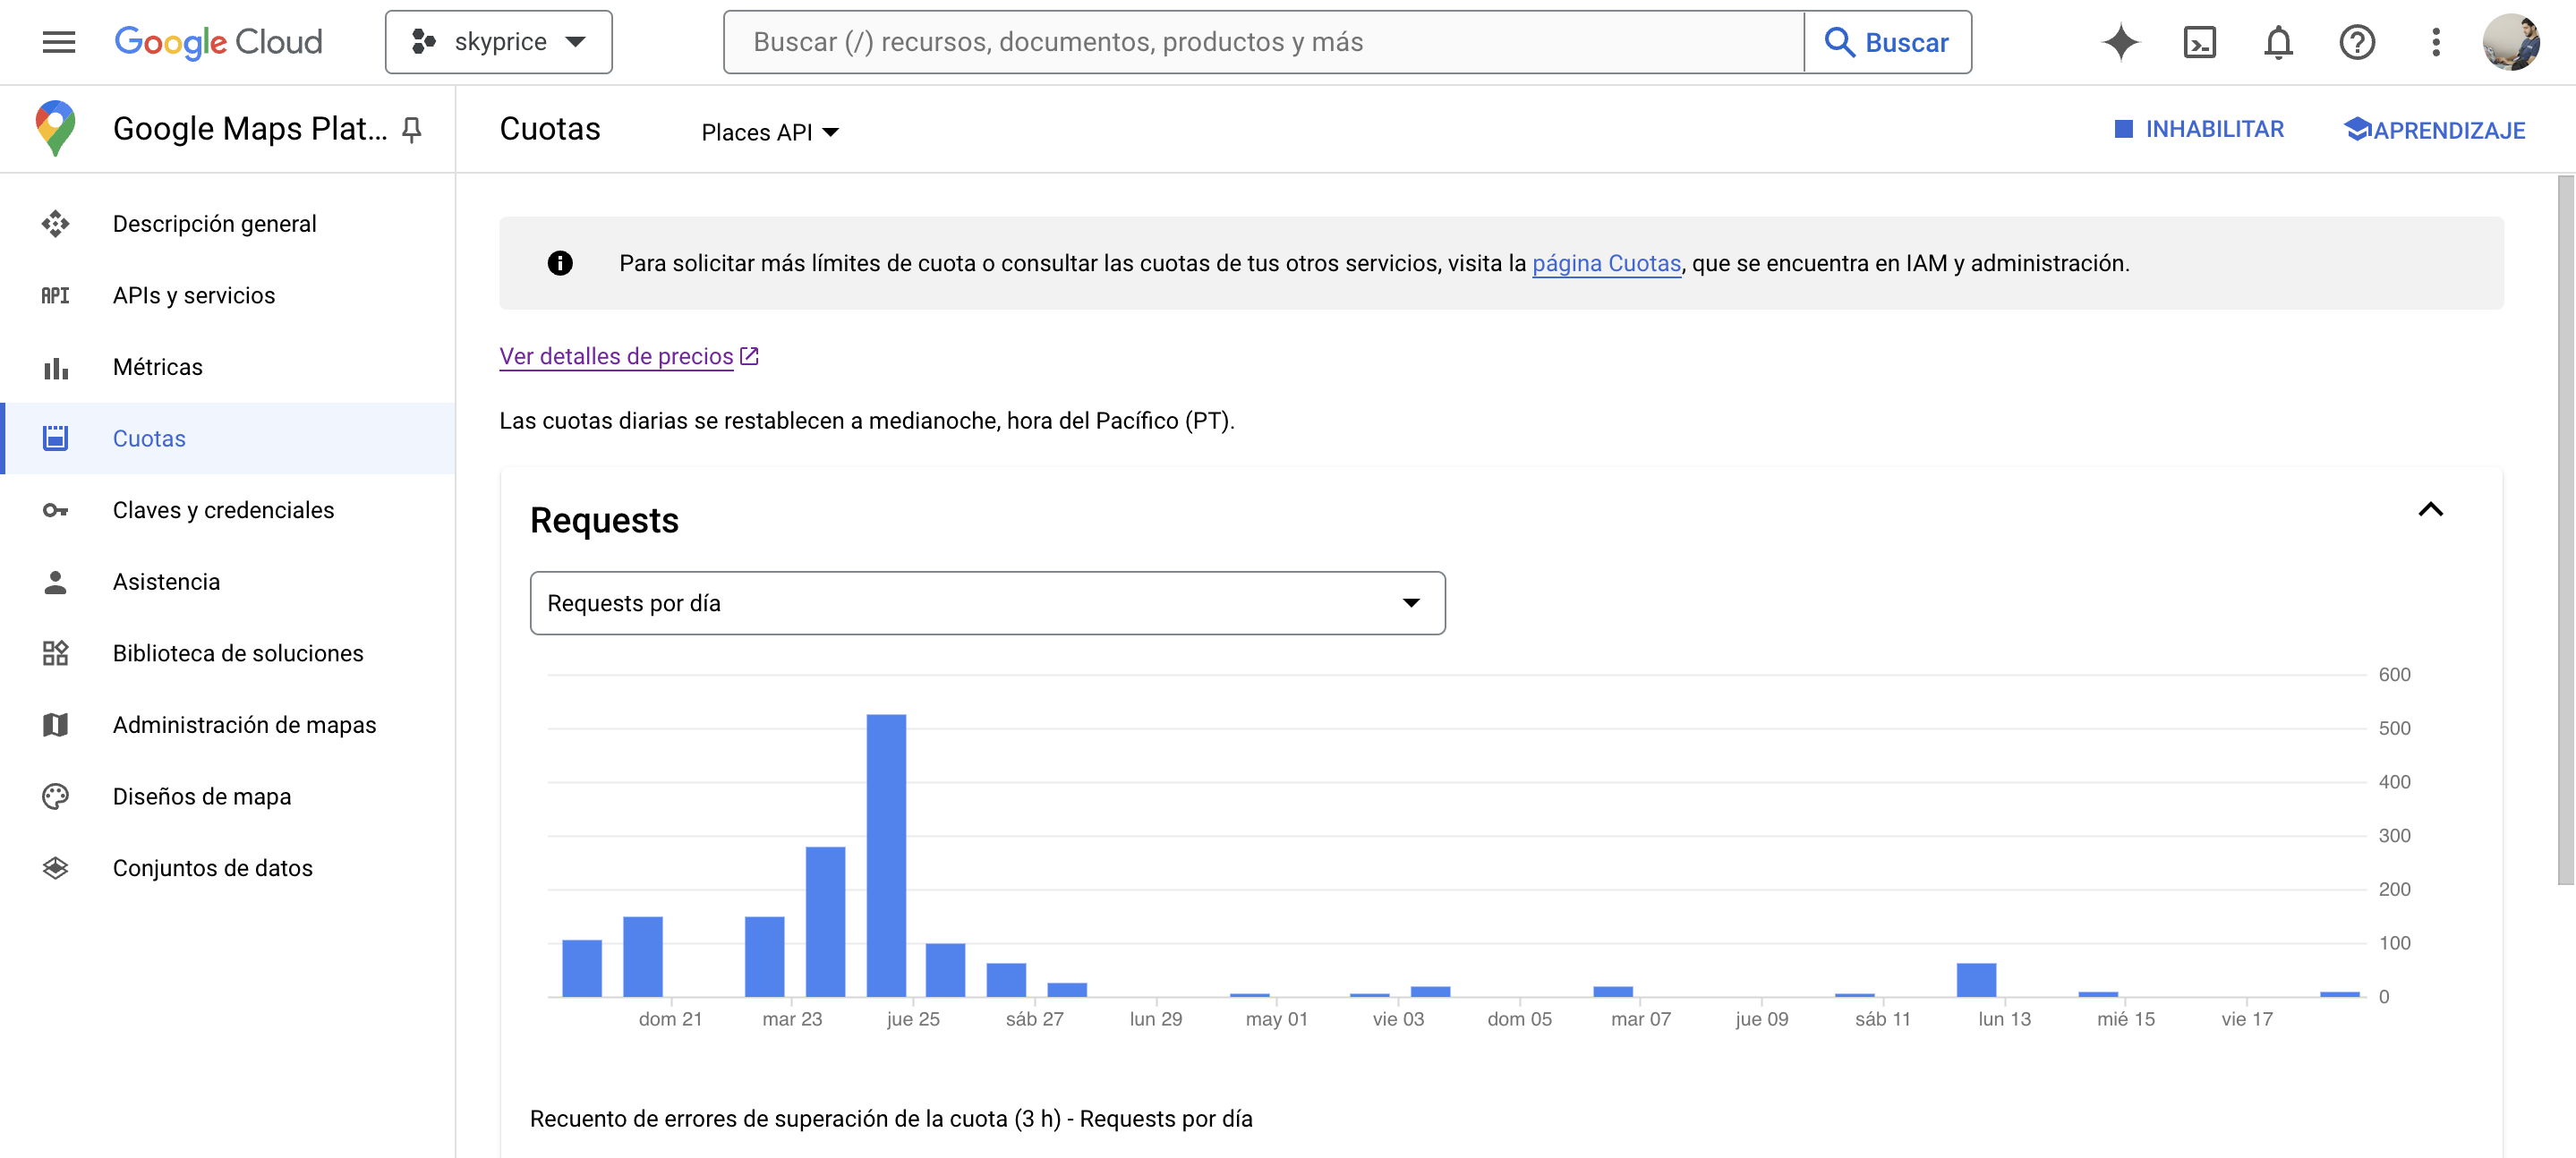
\includegraphics[width=1.0\textwidth]{imagenes/05-implementacion/despliegue/google-maps-api.png}
    \caption{Configuración de la API de Google Maps en Google Cloud.}
    \label{fig:google-maps-api}
\end{figure}

Así, se puede observar que la API se ha configurado exitosamente ya que se muestra
el estado \textit{Habilitado} en la consola de Google Cloud. Además, se puede
observar el consumo de la API en términos de solicitudes.

\subsubsection{ExchangeRate-API}
Se implementó un servicio de conversión de monedas utilizando una API externa,
permitiendo a los usuarios ver los precios en diferentes monedas. Esto es
especialmente útil para usuarios internacionales que deseen ver los precios en
su moneda local. Para ello, se utilizó la API de \textit{ExchangeRate-API}, que
proporciona tasas de cambio en tiempo real y es fácil de integrar en aplicaciones
web y móviles \cite{exchangerate_api}.

En la figura \ref{fig:exchange-rate-api} se muestra la página principal del servicio,
dónde se observan las estadísticas de uso de la API, así como la información de la
cuenta y las opciones de configuración.

\begin{figure}[H]
    \centering
    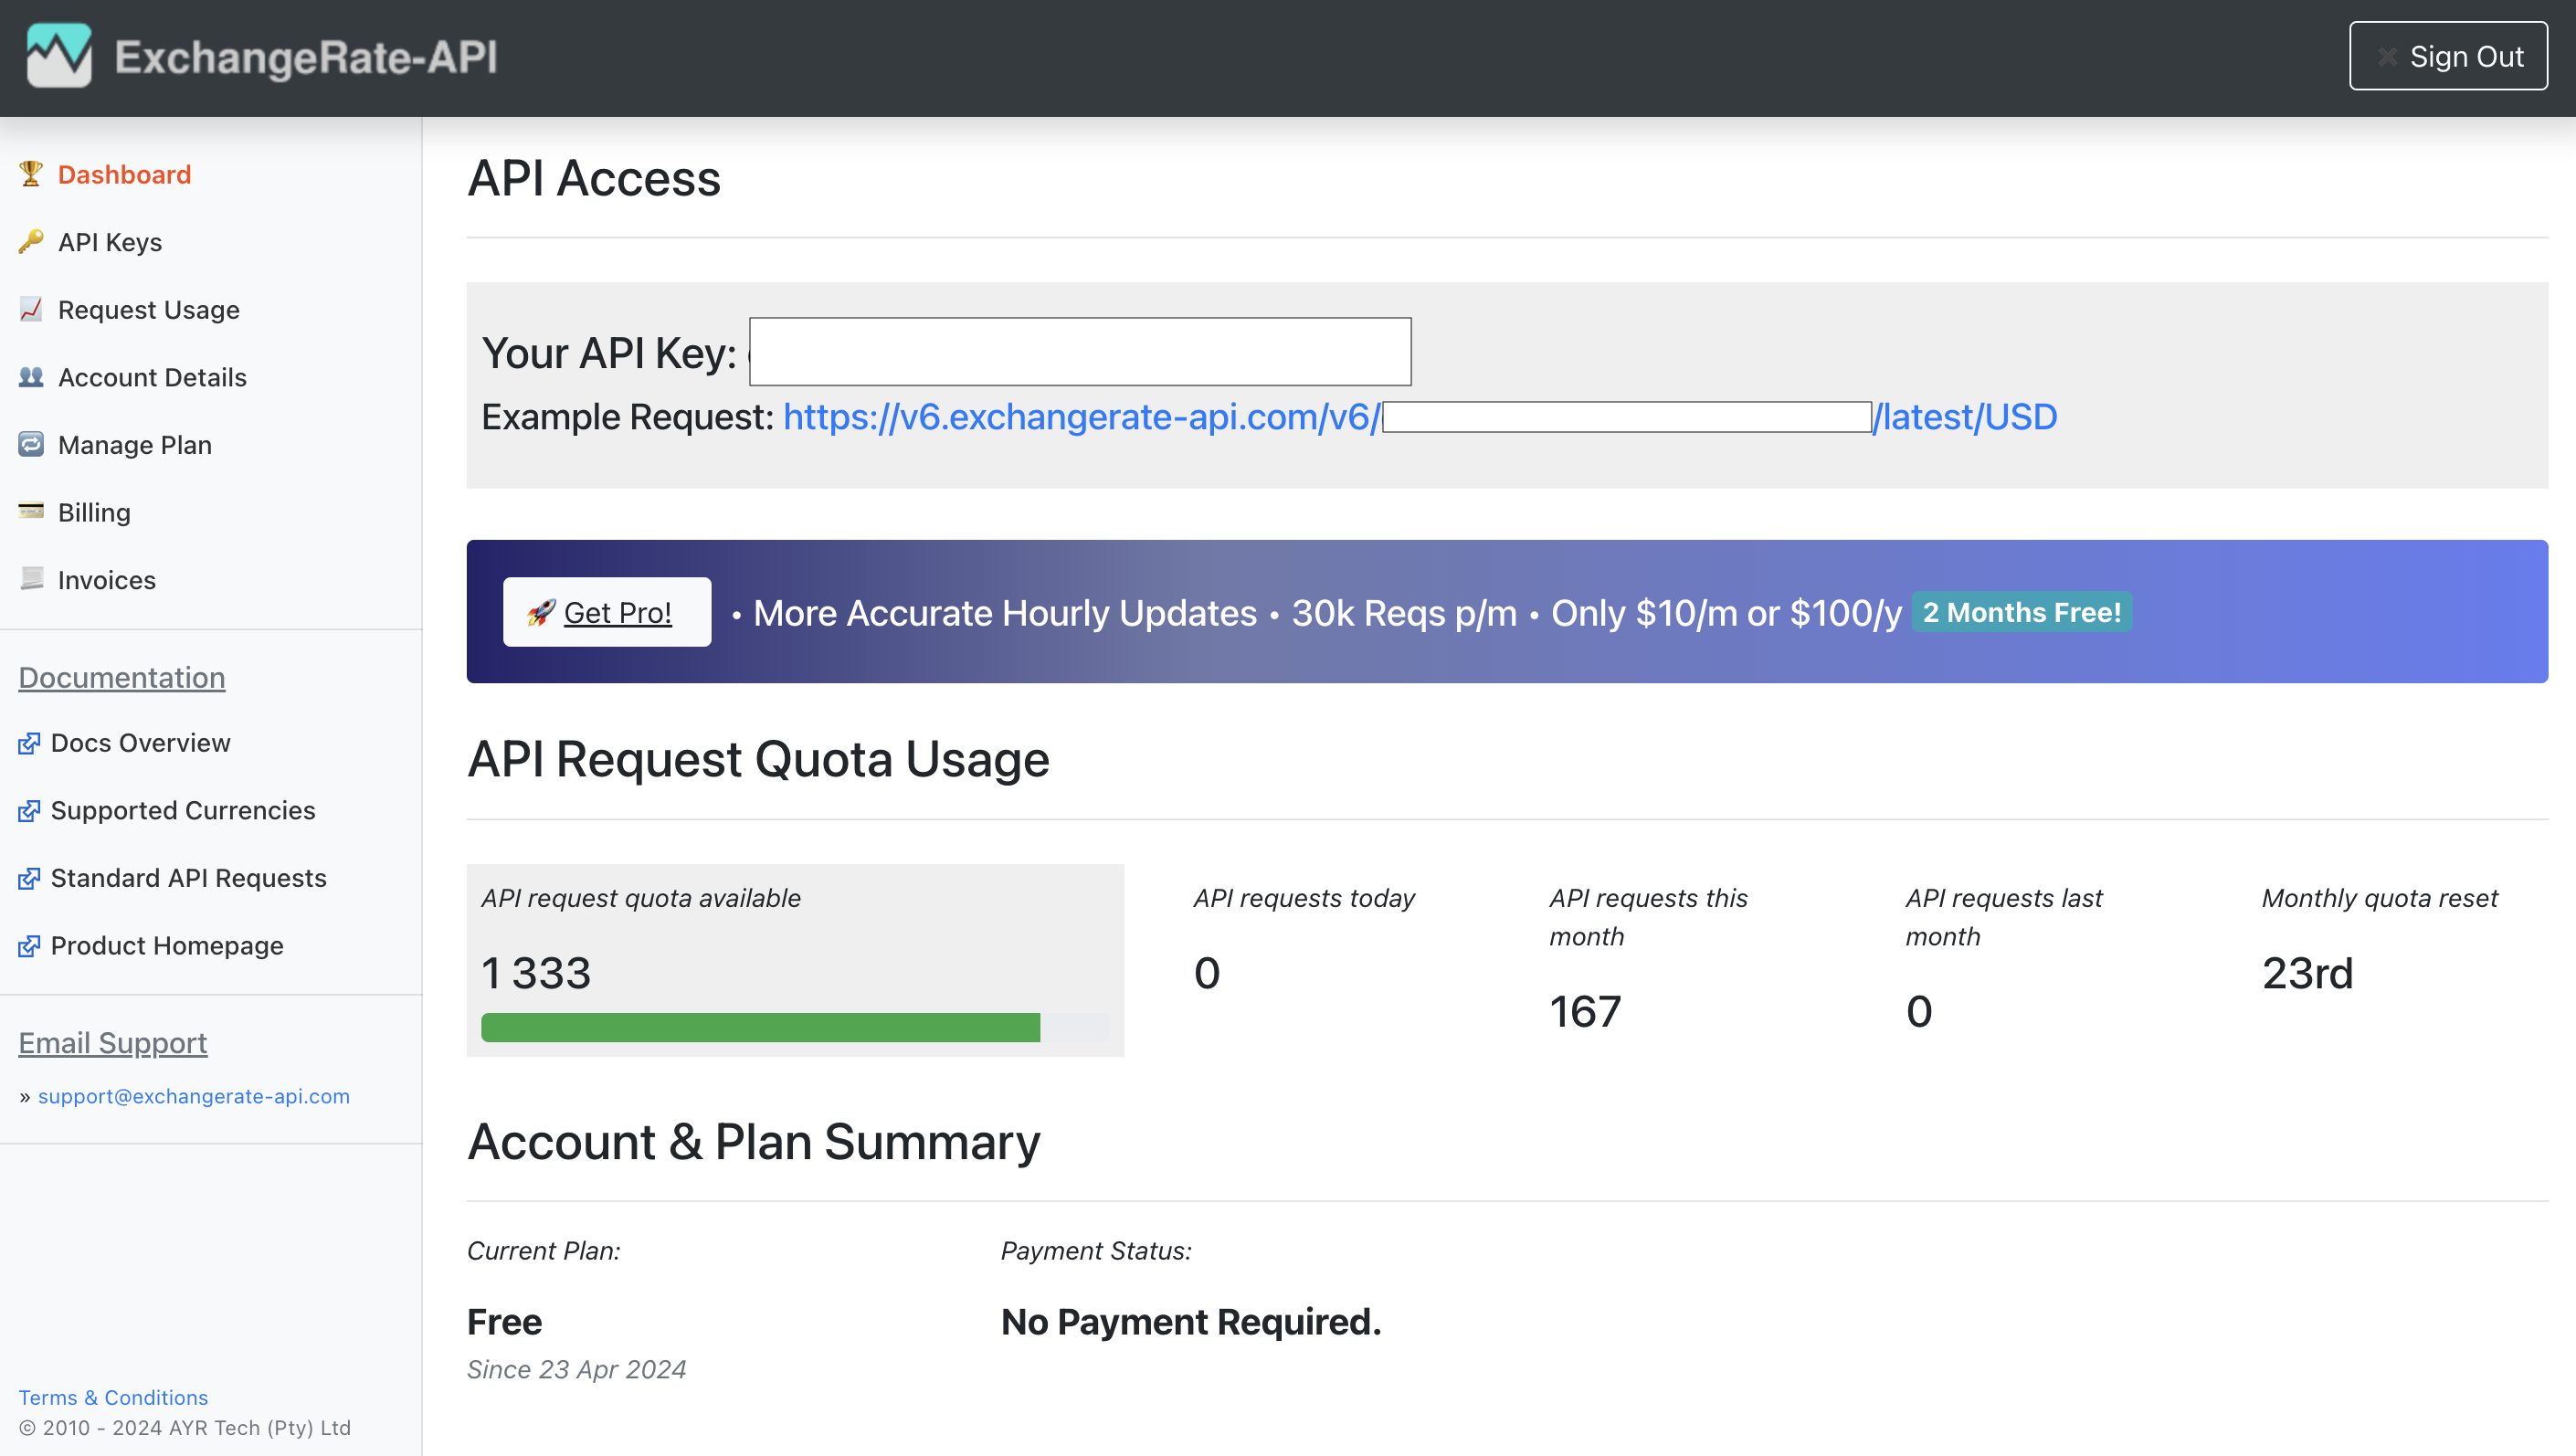
\includegraphics[width=1.0\textwidth]{imagenes/05-implementacion/despliegue/exchangerate-api.png}
    \caption{Página principal de la API de ExchangeRate-API.}
    \label{fig:exchange-rate-api}
\end{figure}

En el listado \ref{lst:currency-converter} se muestra el código requerido para
realizar la conversión de moneda utilizando la API de \textit{ExchangeRate-API}.
En este caso, se utiliza \texttt{fetch} para realizar la petición
HTTP a la API y obtener la tasa de cambio entre la moneda base y la moneda de
interés.

\begin{lstlisting}[language=javascript, caption={Conversión de moneda utilizando la API de ExchangeRate-API}, label={lst:currency-converter}]
useEffect(() => {
  if (currency === 'MXN') {
    setConvertedPrice(price);
    return;
  }
  const fetchData = async () => {
    try {
      const response = await fetch(
        `https://v6.exchangerate-api.com/v6/${
          process.env.NEXT_PUBLIC_EXCHANGERATE_API_KEY || ''
        }/pair/MXN/${currency}/${price}`,
        {
          method: 'GET',
          headers: {
            'Content-Type': 'application/json',
          },
          mode: 'cors',
        },
      );
      const jsonData = await response.json();
      setConvertedPrice(jsonData.conversion_result);
    } catch (error) {
      console.error('Error fetching currency data:', error);
      alert(t('predictionForm.currencyConverter.requestError'));
    }
  };

  fetchData();
}, [currency, price]);
\end{lstlisting}

\section{Pruebas del sistema}
Una vez que la aplicación se ha desplegado en la nube, es importante realizar
pruebas exhaustivas para garantizar que la aplicación funcione correctamente y
cumpla con los requisitos y especificaciones establecidos. En este sentido, se
realizaron pruebas de funcionalidad, rendimiento y seguridad para verificar el
correcto funcionamiento de la aplicación. Además, se utilizaron herramientas
como Google PageSpeed Insights y Google Analytics para evaluar el rendimiento
y la experiencia del usuario.

\subsection{Google Page Speed Insights}
Google PageSpeed Insights es una herramienta que analiza el rendimiento de una
página web tanto en dispositivos móviles como en escritorio. Utiliza Lighthouse
para generar informes detallados y ofrece sugerencias para mejorar la velocidad
y la experiencia del usuario. Lighthouse es una herramienta automatizada de
código abierto que realiza auditorías en las páginas web, evaluando aspectos
como la accesibilidad, el rendimiento, las mejores prácticas y la SEO \cite{google_pagespeed_insights}.
A continuación se presentan los resultados de las pruebas de Google PageSpeed Insights
en la interfaz gráfica de la aplicación tanto en un entorno de escritorio como en
un entorno móvil.

\subsubsection{Escritorio}
En la figura \ref{fig:lighthouse-desktop} se muestra el resultado de las pruebas
de Lighthouse en la interfaz gráfica en un entorno de escritorio. Las puntuaciones
obtenidas muestra un rendimiento, accesibilidad y buenas prácticas sobresalientes.
El SEO obtuvo una puntuación menor debido a la especificación de metadatos que
previenen la indexación de la página.

\begin{figure}[H]
    \centering
    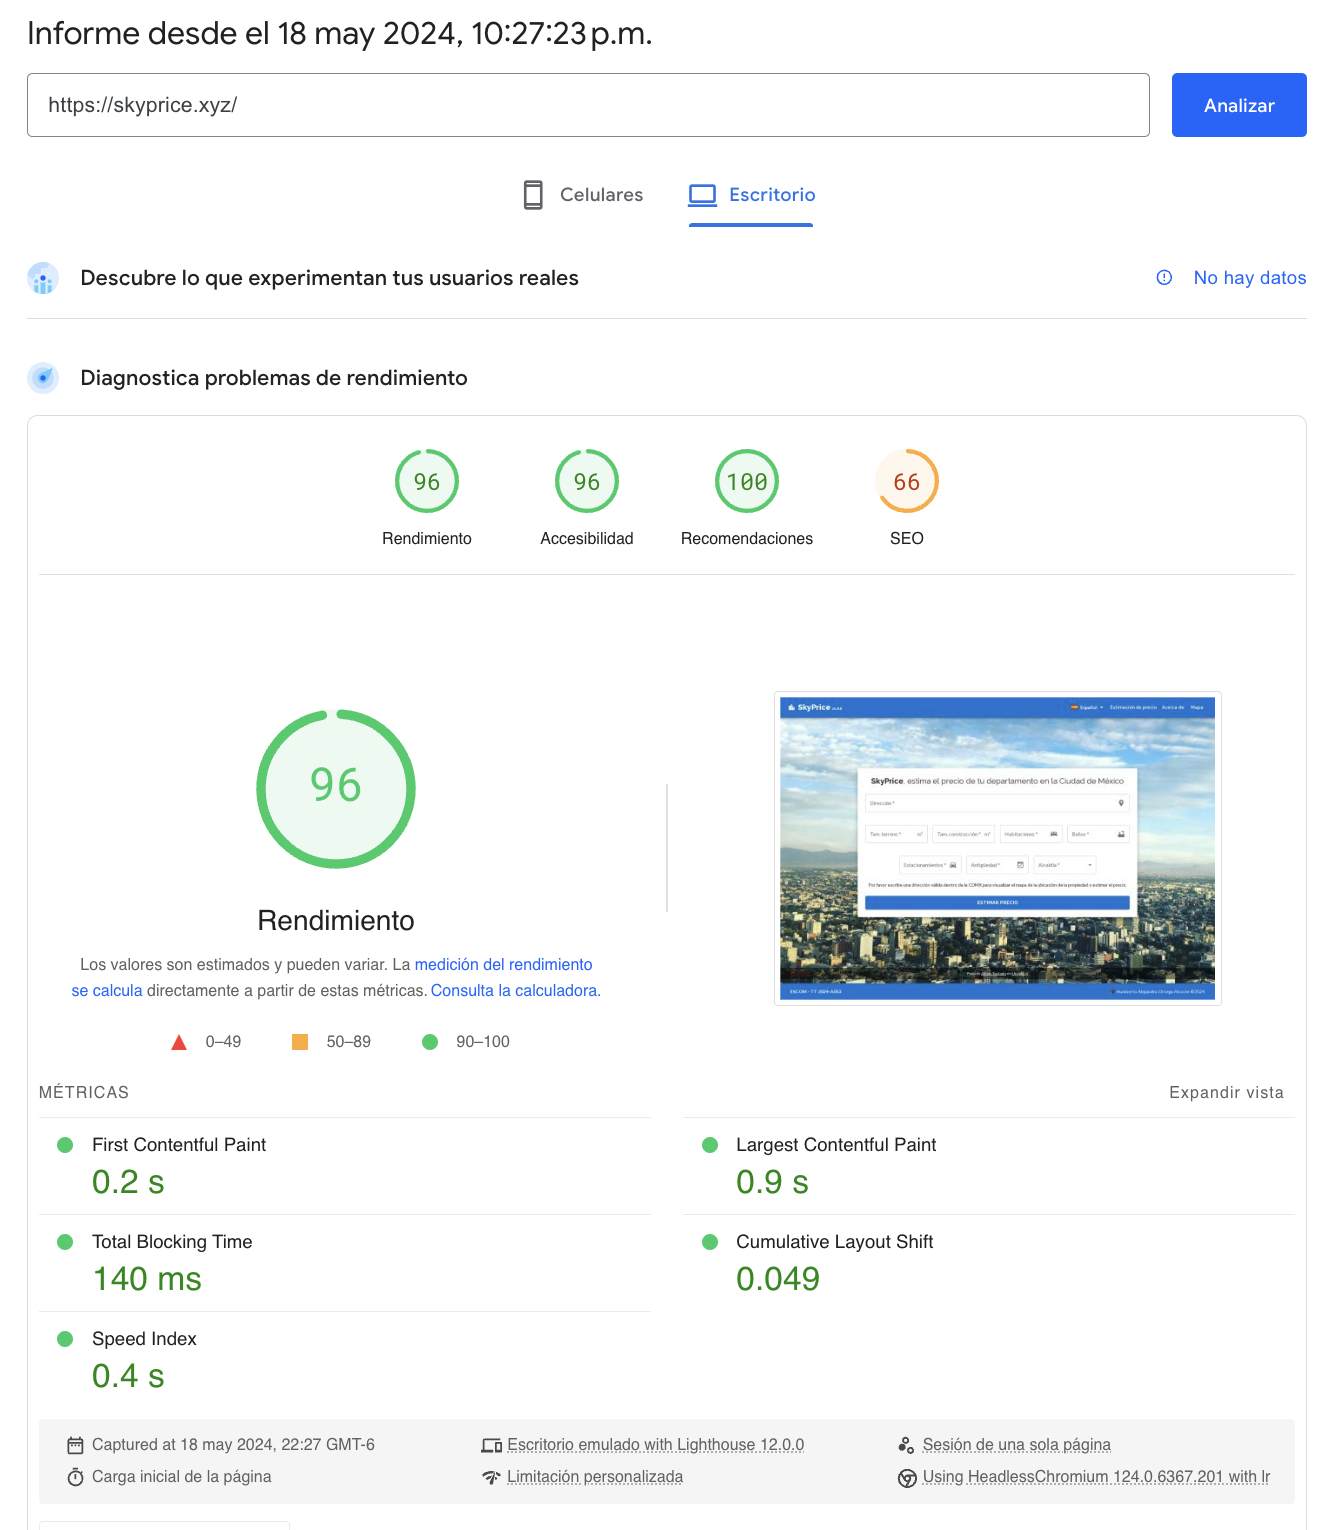
\includegraphics[width=1.0\textwidth]{imagenes/05-implementacion/pruebas/lighthouse-desktop.png}
    \caption{Resultados de las pruebas de Lighthouse en un entorno de escritorio.}
    \label{fig:lighthouse-desktop}
\end{figure}

\subsubsection{Móvil}
En la figura \ref{fig:lighthouse-mobile} se muestra el resultado de las pruebas
de Lighthouse en la interfaz gráfica en un entorno móvil. Las puntuaciones obtenidas
muestran un rendimiento malo debido a la falta de compresión de imágenes, la
accesibilidad y las buenas prácticas son sobresalientes, y el SEO obtuvo una puntuación
menor debido a la especificación de metadatos que previenen la indexación de la página.

\begin{figure}[H]
    \centering
    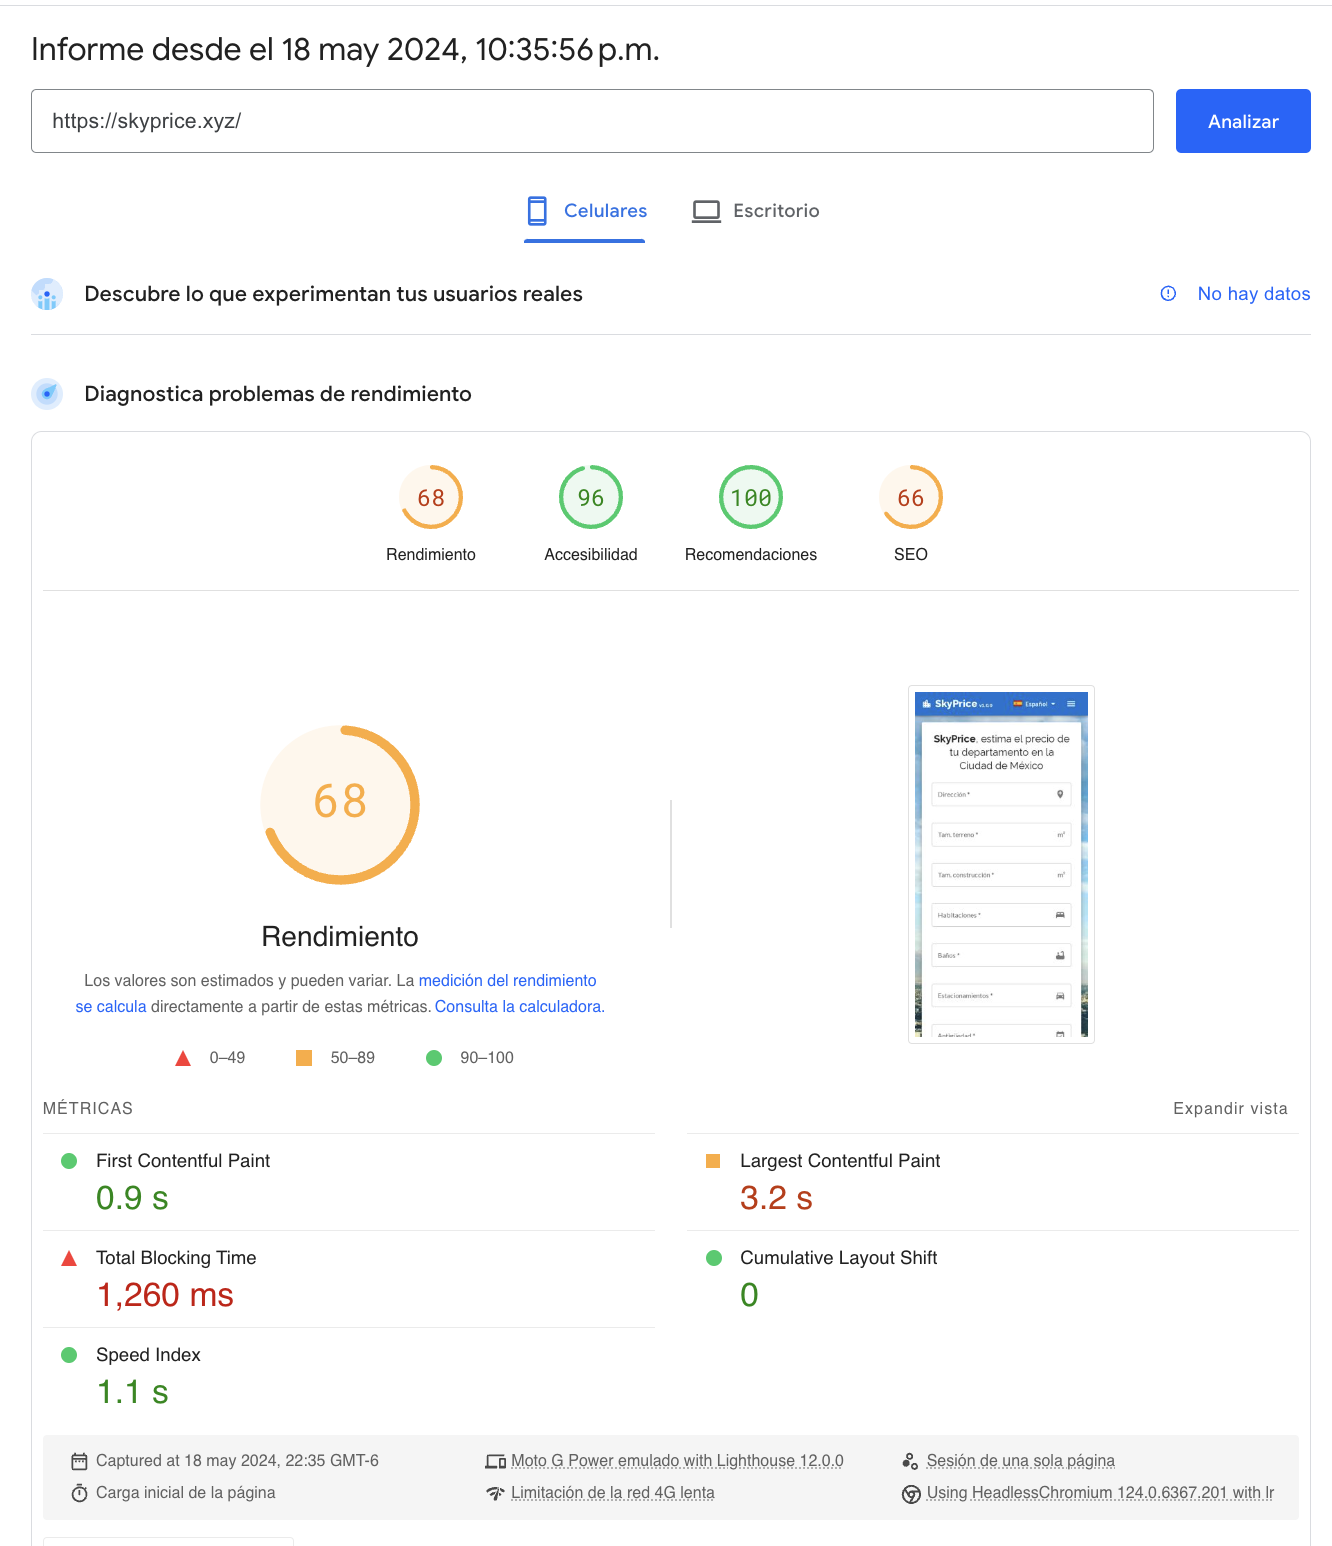
\includegraphics[width=1.0\textwidth]{imagenes/05-implementacion/pruebas/lighthouse-mobile.png}
    \caption{Resultados de las pruebas de Lighthouse en un entorno móvil.}
    \label{fig:lighthouse-mobile}
\end{figure}

Es importante destacar que las puntuaciones obtenidas en las pruebas anteriores
no son definitivas y pueden variar dependiendo de factores ajenos al desarrollo
de la aplicación, como la velocidad de la conexión a Internet, la ubicación geográfica
del usuario, el dispositivo utilizado, entre otros.

\subsection{Google Analytics}
Google Analytics es una plataforma de análisis web que ofrece herramientas para
medir el tráfico y el rendimiento del sitio web. Proporciona informes detallados
sobre cómo los usuarios interactúan con el sitio, permitiendo a los administradores
web y a los desarrolladores comprender mejor el comportamiento de los usuarios.
Con Google Analytics, es posible rastrear diversas métricas, como la cantidad de
visitantes, las páginas más vistas, las tasas de conversión y la efectividad de
campañas publicitarias. Esta información es crucial para optimizar la experiencia
del usuario y tomar decisiones informadas basadas en datos \cite{google_analytics_learn}.

En la figura \ref{fig:google-analytics} se muestra la página principal de Google
Analytics con información sobre el tráfico del sitio web. En este caso, se puede
observar el número de usuarios activos, las páginas más visitadas, la tasa de rebote
y la duración promedio de la sesión. Esta información es valiosa para evaluar el
rendimiento del sitio web y realizar ajustes en función de los datos obtenidos.

\begin{figure}[H]
    \centering
    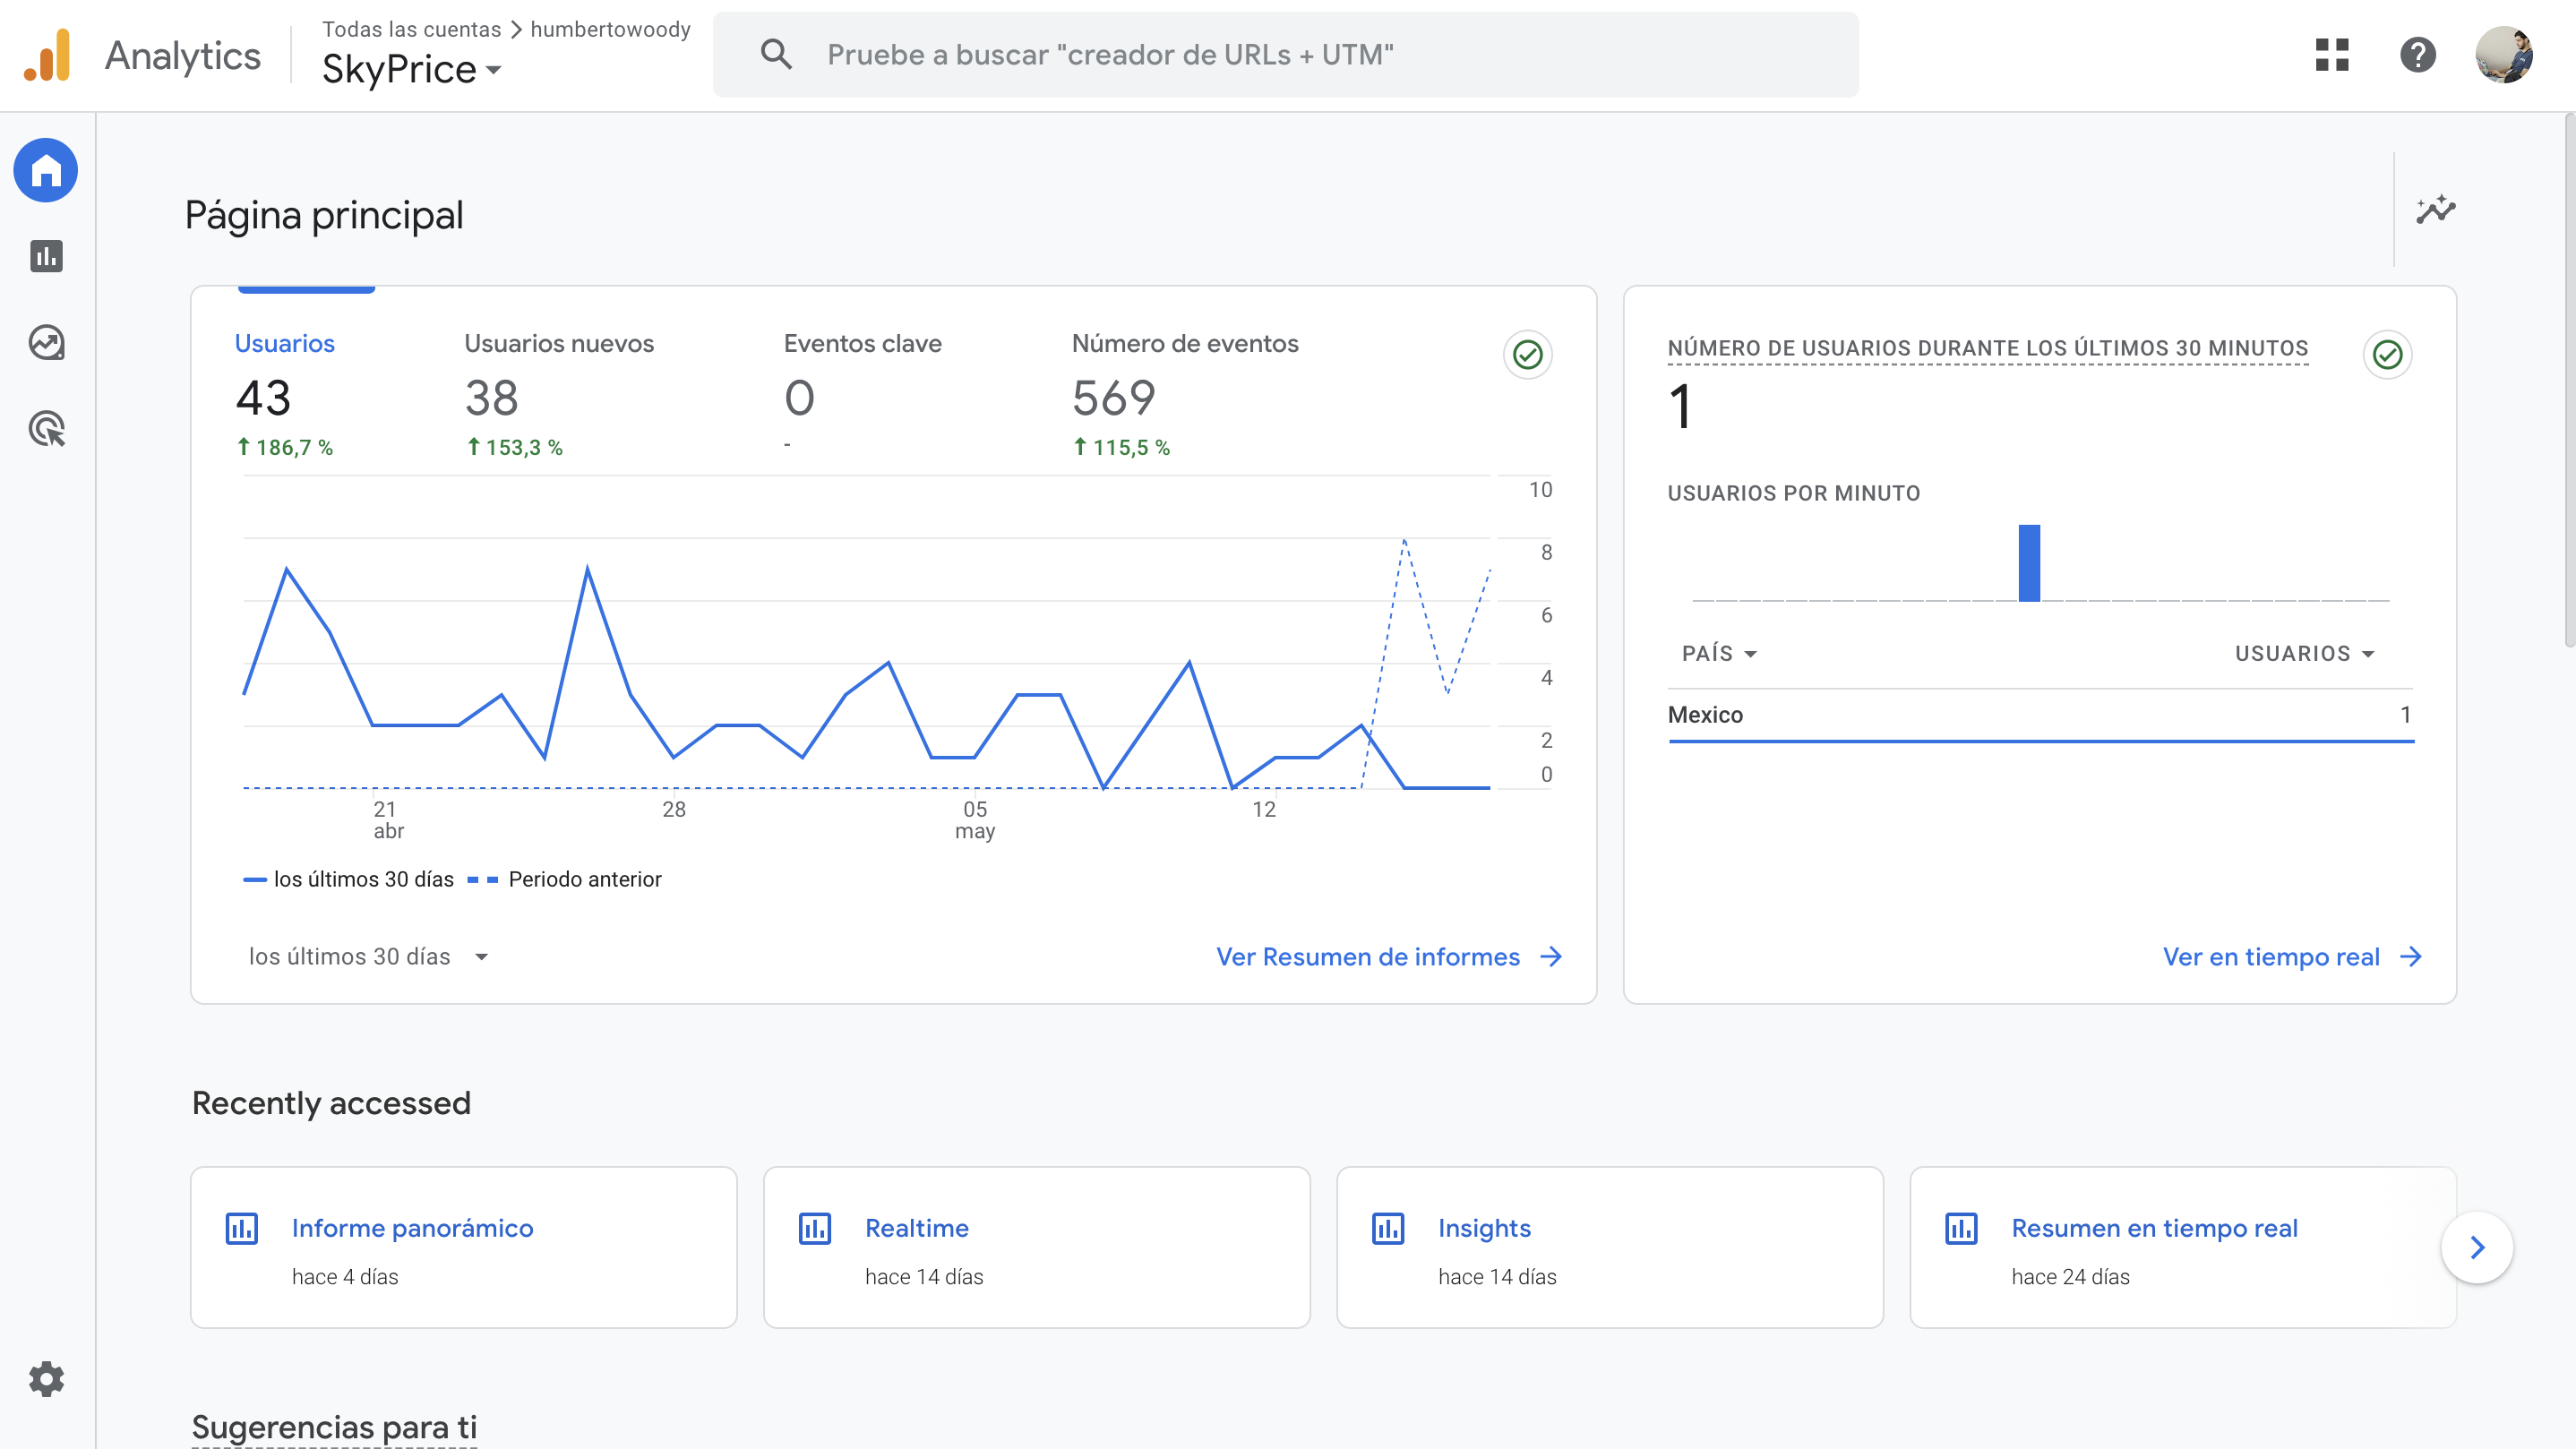
\includegraphics[width=1.0\textwidth]{imagenes/05-implementacion/pruebas/analytics-main.png}
    \caption{Página principal de Google Analytics con información sobre el tráfico del sitio web.}
    \label{fig:google-analytics}
\end{figure}

Para integrar Google Analytics en la interfaz gráfica de la aplicación, se utilizó
Google Tag Manager, una herramienta que permite gestionar y desplegar etiquetas de
seguimiento en un sitio web de manera sencilla y eficiente. En el listado
\ref{lst:google-tag-manager} se muestra el fragmento de código que se incluyó en
la interfaz gráfica para integrar Google Tag Manager. Este código corresponde
al componente principal de la aplicación, y garantiza que Google Analytics se
cargue en todas las páginas del sitio web.

\begin{lstlisting}[language=javascript, caption={Fragmento de código para Google Tag Manager}, label={lst:google-tag-manager}]
export default function RootLayout(props: { children: React.ReactNode }) {
  const urlgtm: string = `https://www.googletagmanager.com/gtag/js?id=${process.env.NEXT_PUBLIC_GOOGLE_ANALYTICS}`;
  return (
    <html lang="en">
      <Script src={urlgtm} />
      <Script>
        {`
            window.dataLayer = window.dataLayer || [];
            function gtag(){dataLayer.push(arguments);}
            gtag('js', new Date());
            gtag('config', '${process.env.NEXT_PUBLIC_GOOGLE_ANALYTICS}');
          `}
      </Script>
      <body>
        <AppRouterCacheProvider options={{ enableCssLayer: true }}>
          <ThemeProvider theme={theme}>
            {/* CssBaseline kickstart an elegant, consistent, and simple baseline to build upon. */}
            <CssBaseline />
            <I18nProvider>{props.children}</I18nProvider>
          </ThemeProvider>
        </AppRouterCacheProvider>
      </body>
    </html>
  );
}
\end{lstlisting}

\subsubsection{Información sobre los usuarios}
Los resultados de Google Analytics proporcionan información detallada sobre los
usuarios que visitan el sitio web. En la figura \ref{fig:google-analytics-usuarios}
se muestra un resumen de la información sobre los usuarios, incluyendo la cantidad
de usuarios activos, las sesiones, la duración promedio de la sesión y la tasa de rebote.

\begin{figure}[H]
    \centering
    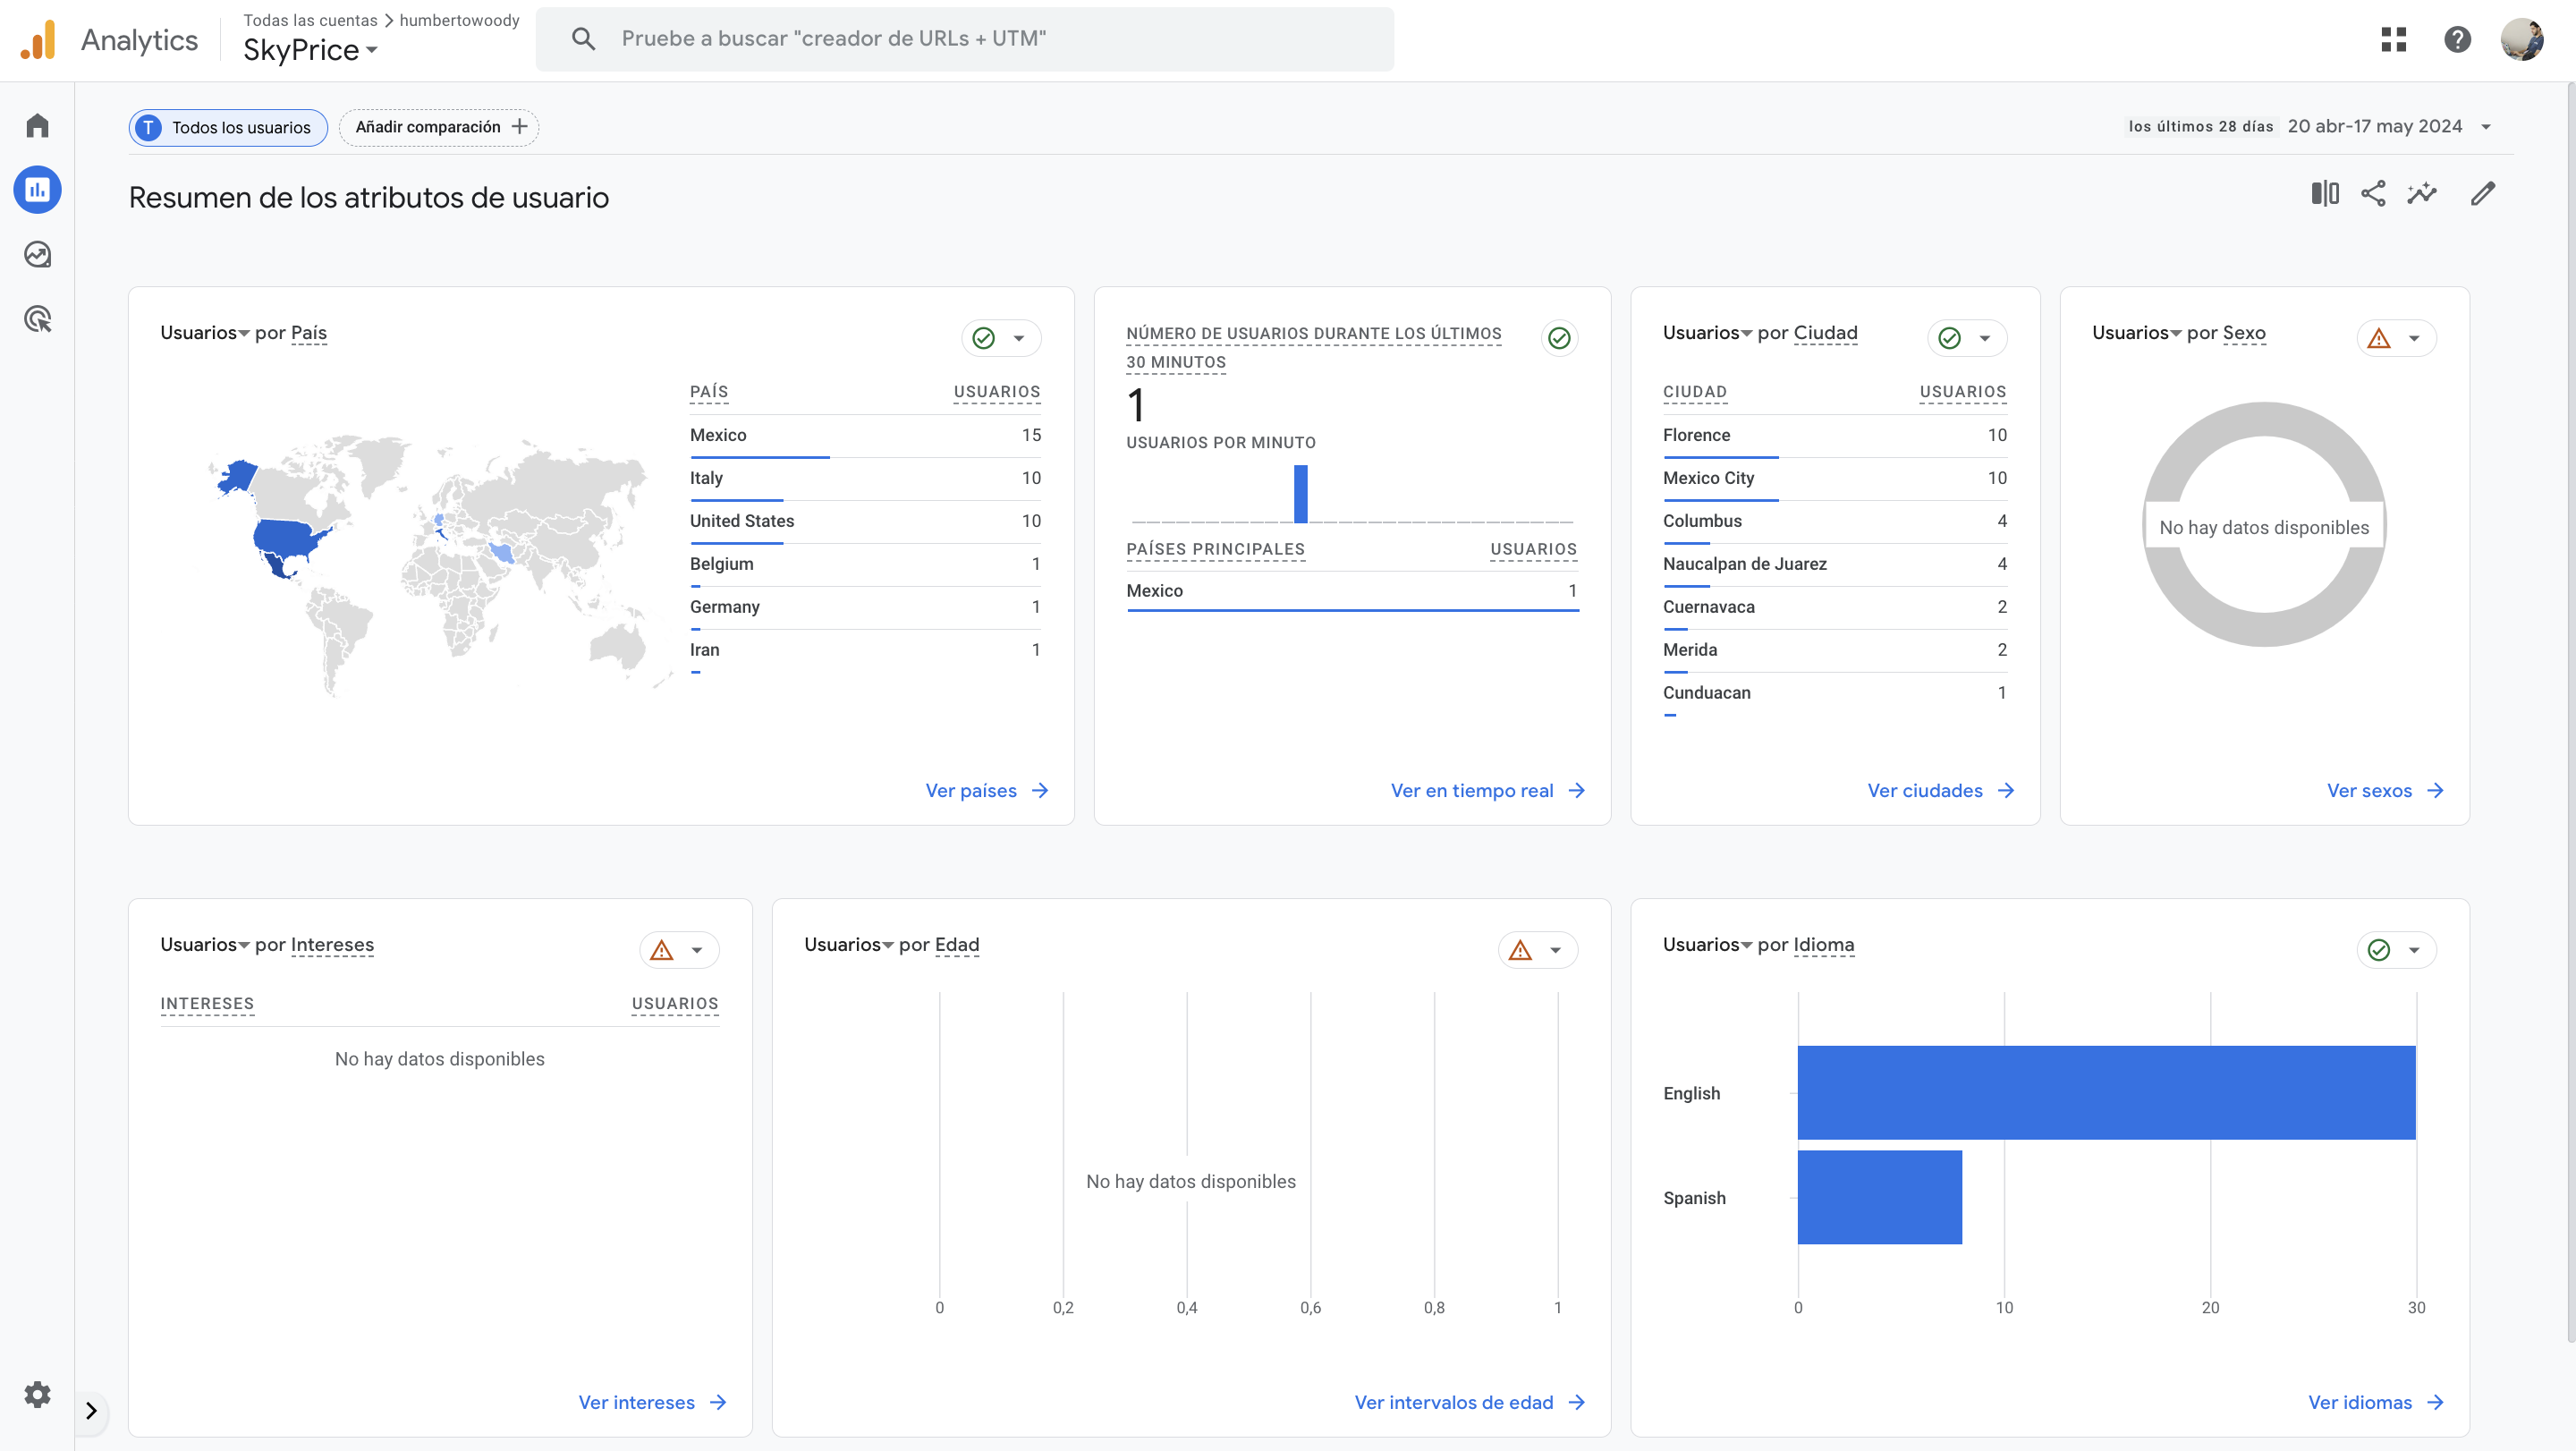
\includegraphics[width=1.0\textwidth]{imagenes/05-implementacion/pruebas/analytics-users.png}
    \caption{Información sobre los usuarios que visitan el sitio web.}
    \label{fig:google-analytics-usuarios}
\end{figure}

\subsubsection{Información sobre la tecnología}
Google Analytics también proporciona información sobre la tecnología utilizada por
los usuarios para acceder al sitio web. En la figura \ref{fig:google-analytics-tecnologia}
se muestra un resumen de la información sobre la tecnología, incluyendo el tipo de
dispositivo, el sistema operativo y el navegador utilizado por los usuarios.

\begin{figure}[H]
    \centering
    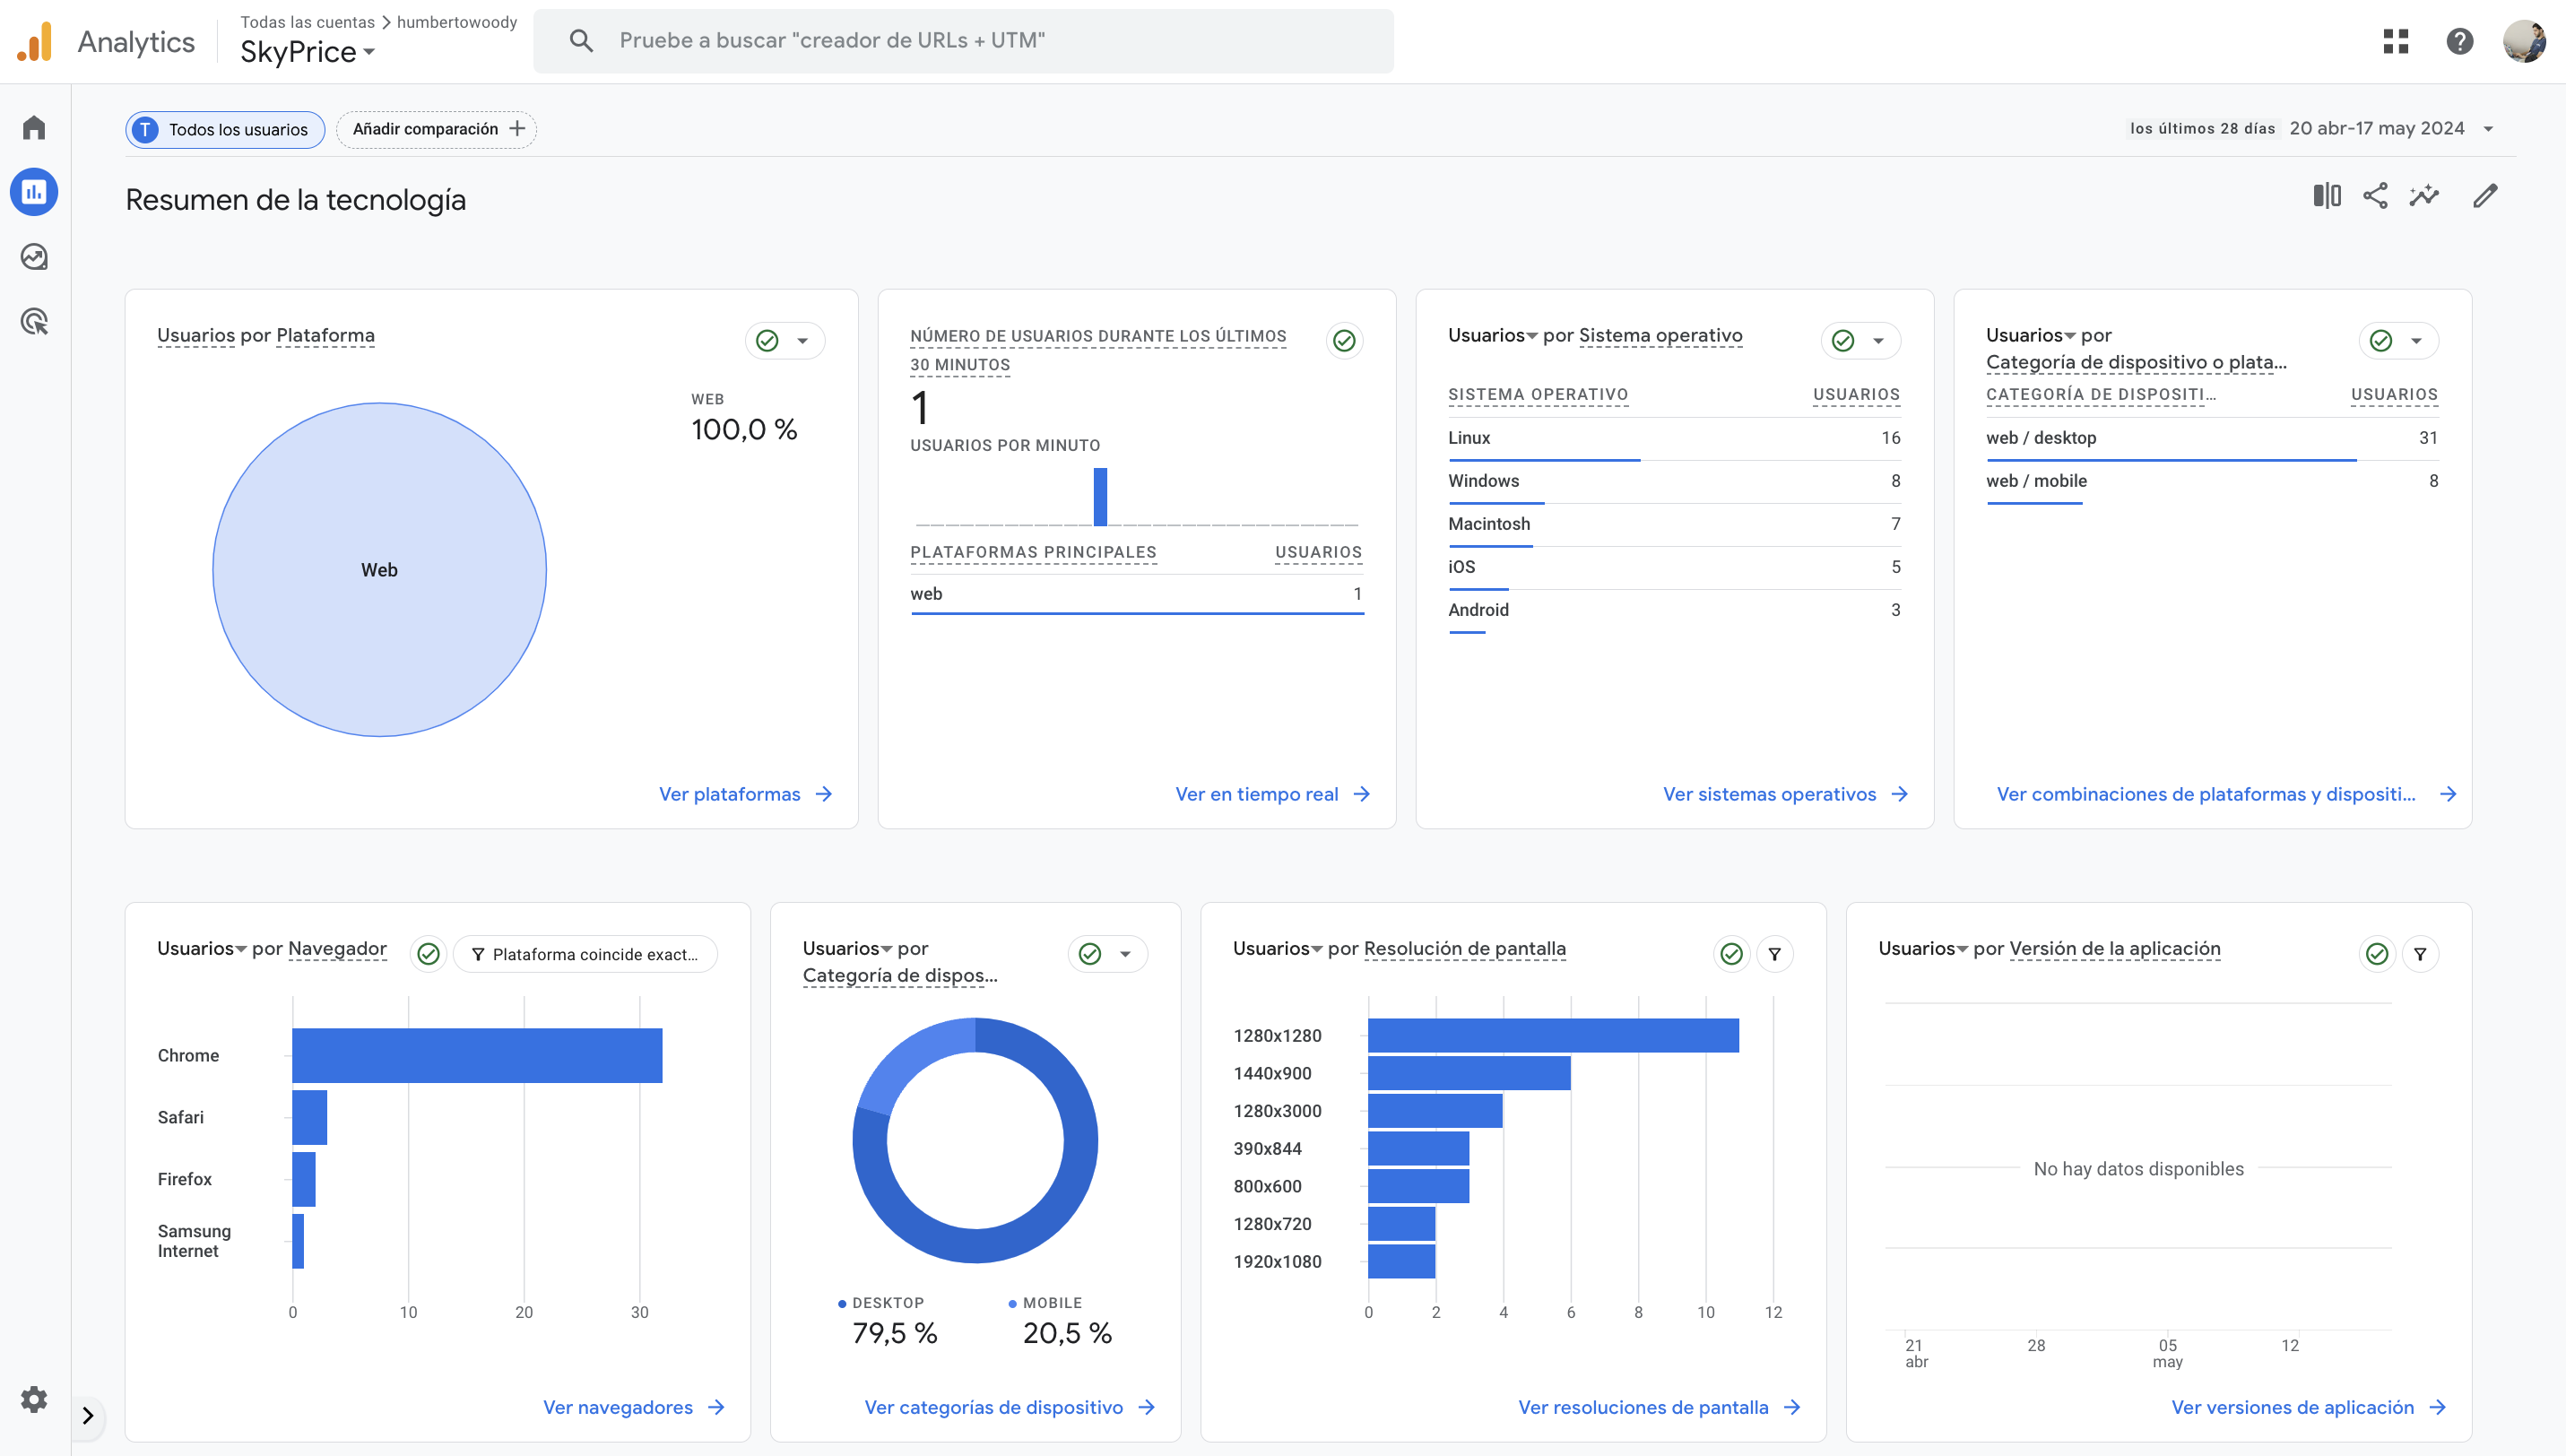
\includegraphics[width=1.0\textwidth]{imagenes/05-implementacion/pruebas/analytics-tech.png}
    \caption{Información sobre la tecnología utilizada por los usuarios para acceder al sitio web.}
    \label{fig:google-analytics-tecnologia}
\end{figure}

\section{Costos}
La operación de SkyPrice implica costos asociados al despliegue de la aplicación
y los servicios externos involucrados. En esta sección se presentan los costos
asociados al despliegue y ejecución de la aplicación en el entorno de AWS, así como
de servicios externos como Google Maps y ExchangeRate-API.

\subsection{AWS}
El despliegue de la aplicación en la nube se realizó el día 8 de Abril del 2024,
con esto se cuenta con un mes de uso de los servicios de AWS lo cual nos
permite observar costes finales de operación. En la figura \ref{fig:costos-diarios}
se muestra el costo diario de la aplicación, incluyendo servicios como Elastic Beanstalk,
S3, CloudFront, Certificate Manager, entre otros.

\begin{figure}[H]
    \centering
    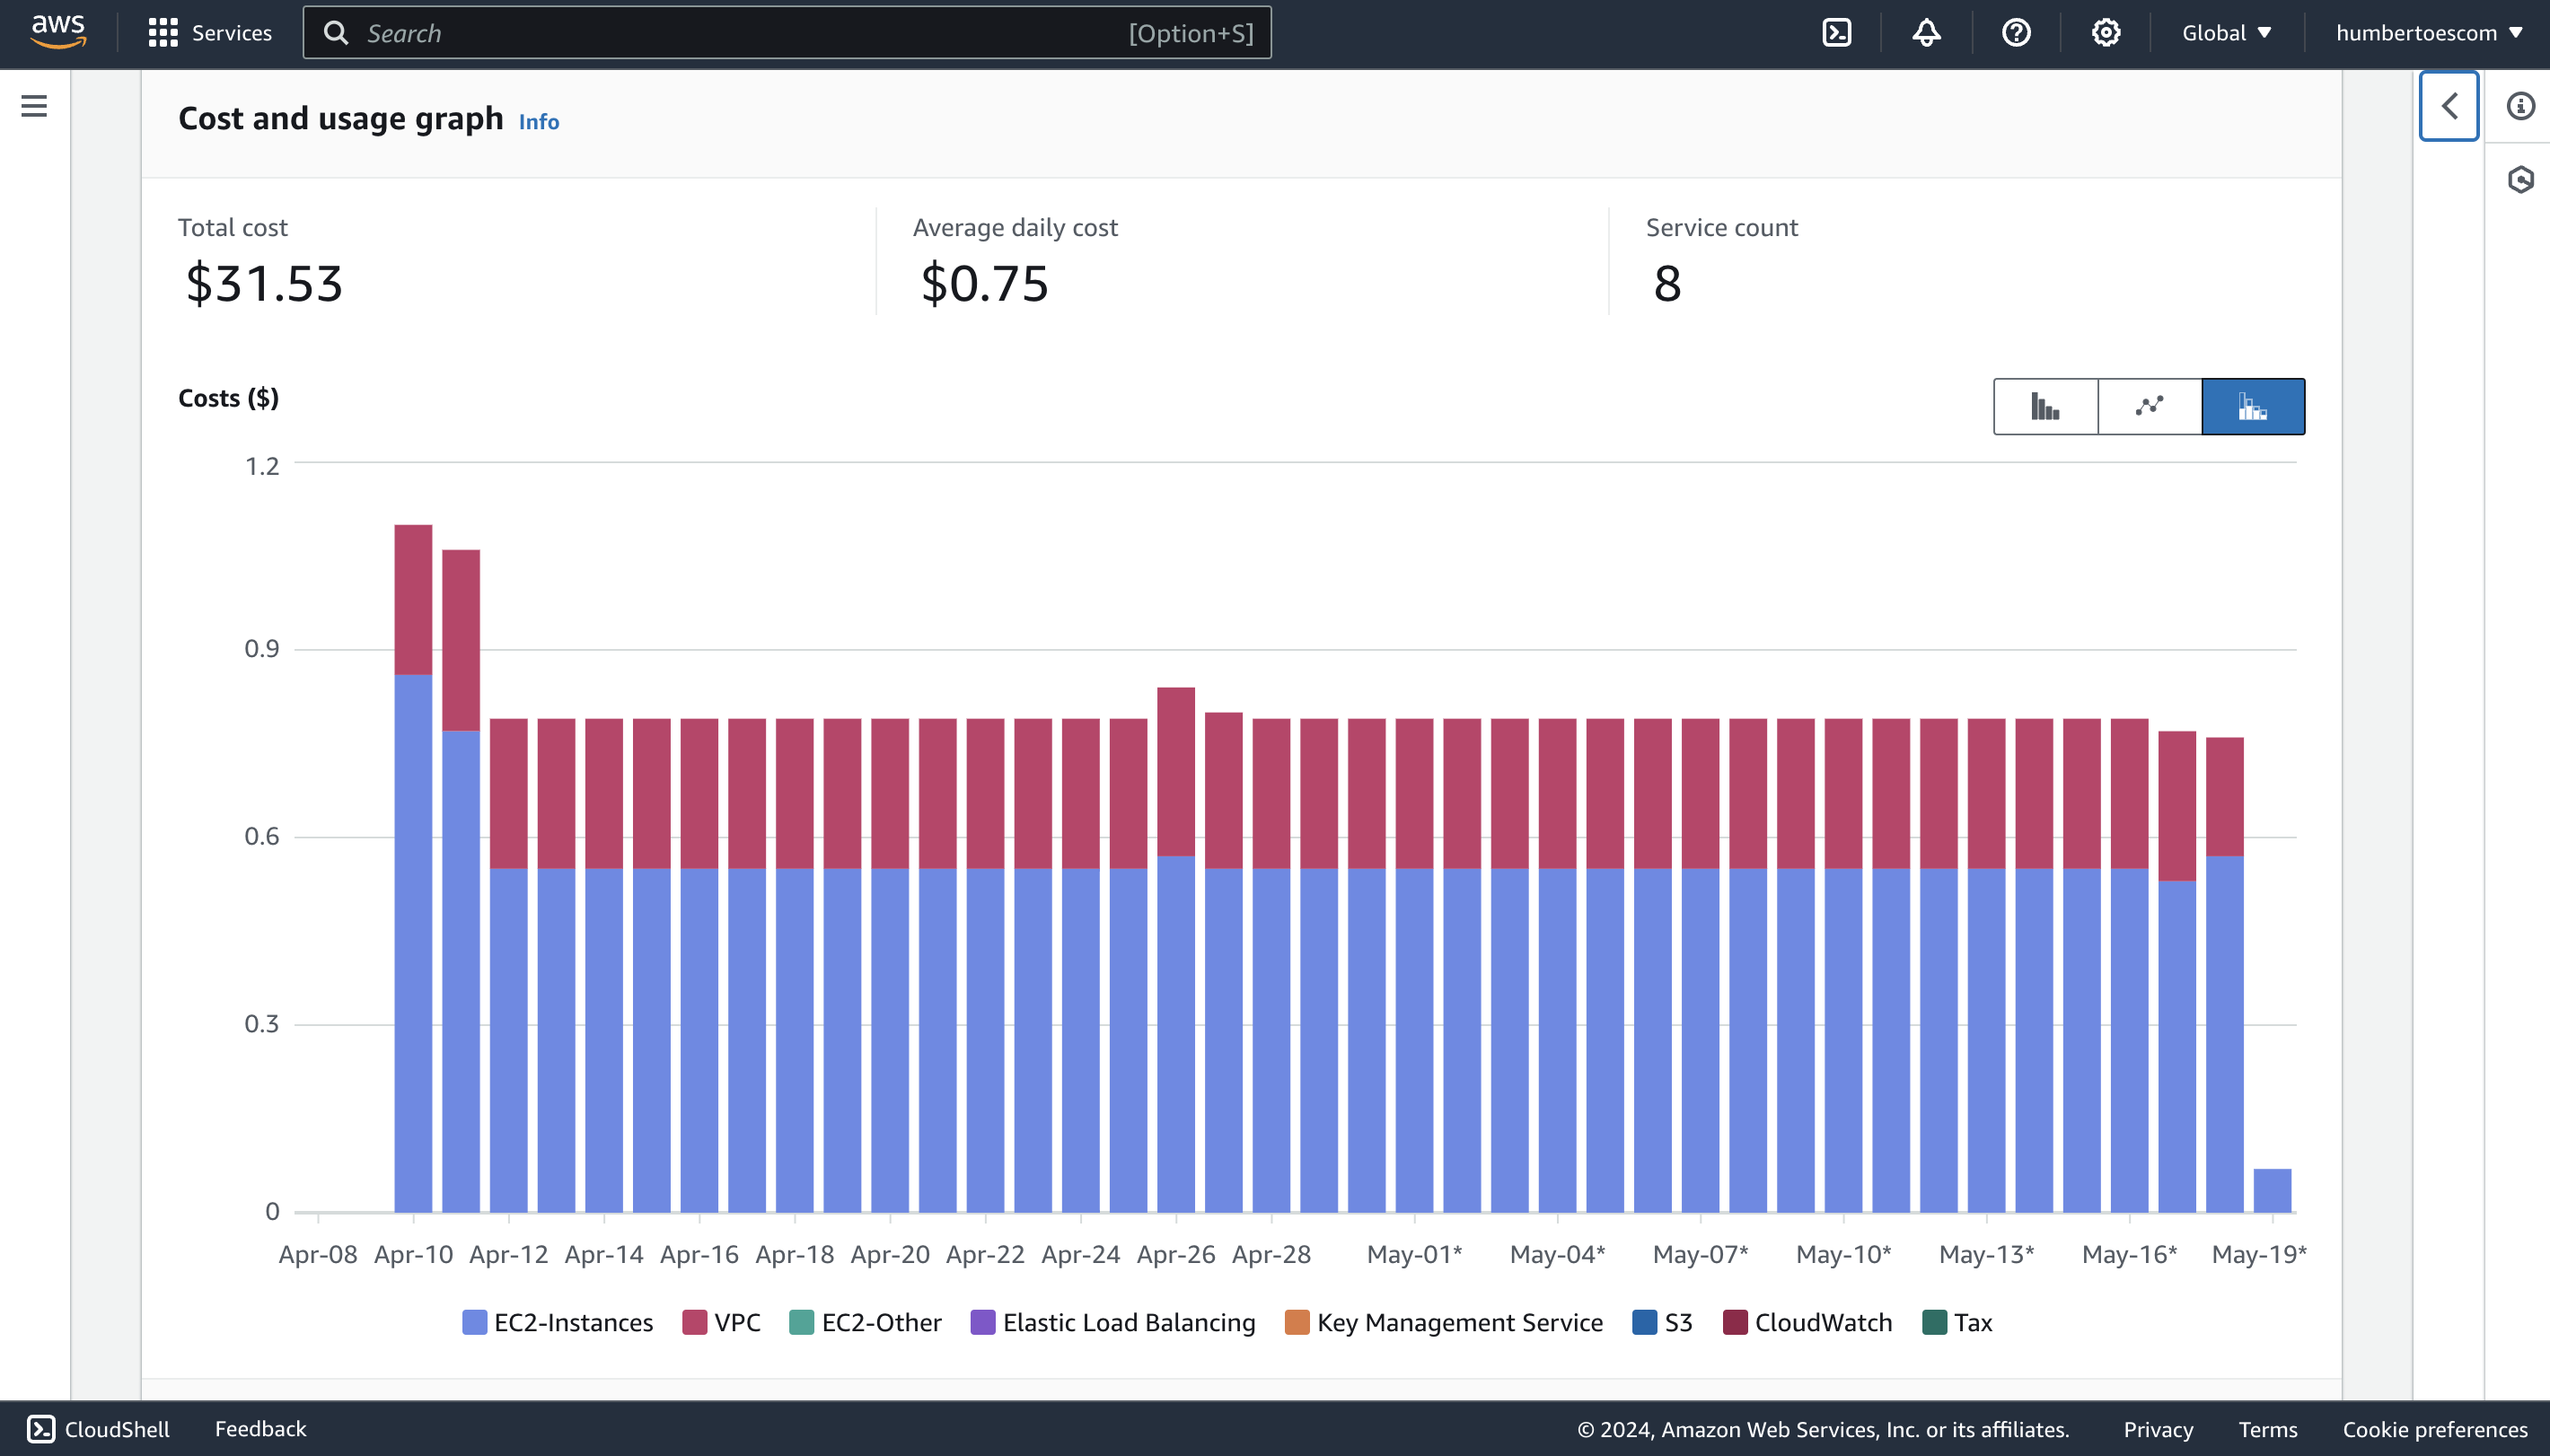
\includegraphics[width=1.0\textwidth]{imagenes/05-implementacion/costos/costos-diarios.png}
    \caption{Costos diarios de la aplicación en la nube.}
    \label{fig:costos-diarios}
\end{figure}

Puede destacarse que los dos servicios que más consumen recursos son Elastic Beanstalk,
con EC2 que es el servicio de cómputo, con un costo de \$0.50 USD diarios y el
tráfico de VPC que es el tráfico de red, con un costo de \$0.24 USD diarios,
estimando un costo total de \$0.75 USD diarios (el centavo extra se compone de cargos
para el resto de servicios implicados). Esto nos da un costo mensual
de \$15.77 USD (~\$265.00 MXN), lo cual es un costo accesible para el mantenimiento de la aplicación
y queda muy por debajo de las estimaciones realizadas.

\subsection{Google Maps}
El uso de la API de Google Maps para la geocodificación de direcciones implica
un coste fijo por petición de dirección geocodificada de \$0.005 USD. Al igual
que AWS, la cuenta de Google Cloud ofrece un crédito inicial de \$300 USD para
nuevos usuarios, lo cual permite realizar un número considerable de peticiones
sin coste adicional. En la figura \ref{fig:costos-google-maps} se muestra el
costo registrado desde el día 8 de Abril del 2024 que es el día en que se realizó
el despliegue de la aplicación.

\begin{figure}[H]
    \centering
    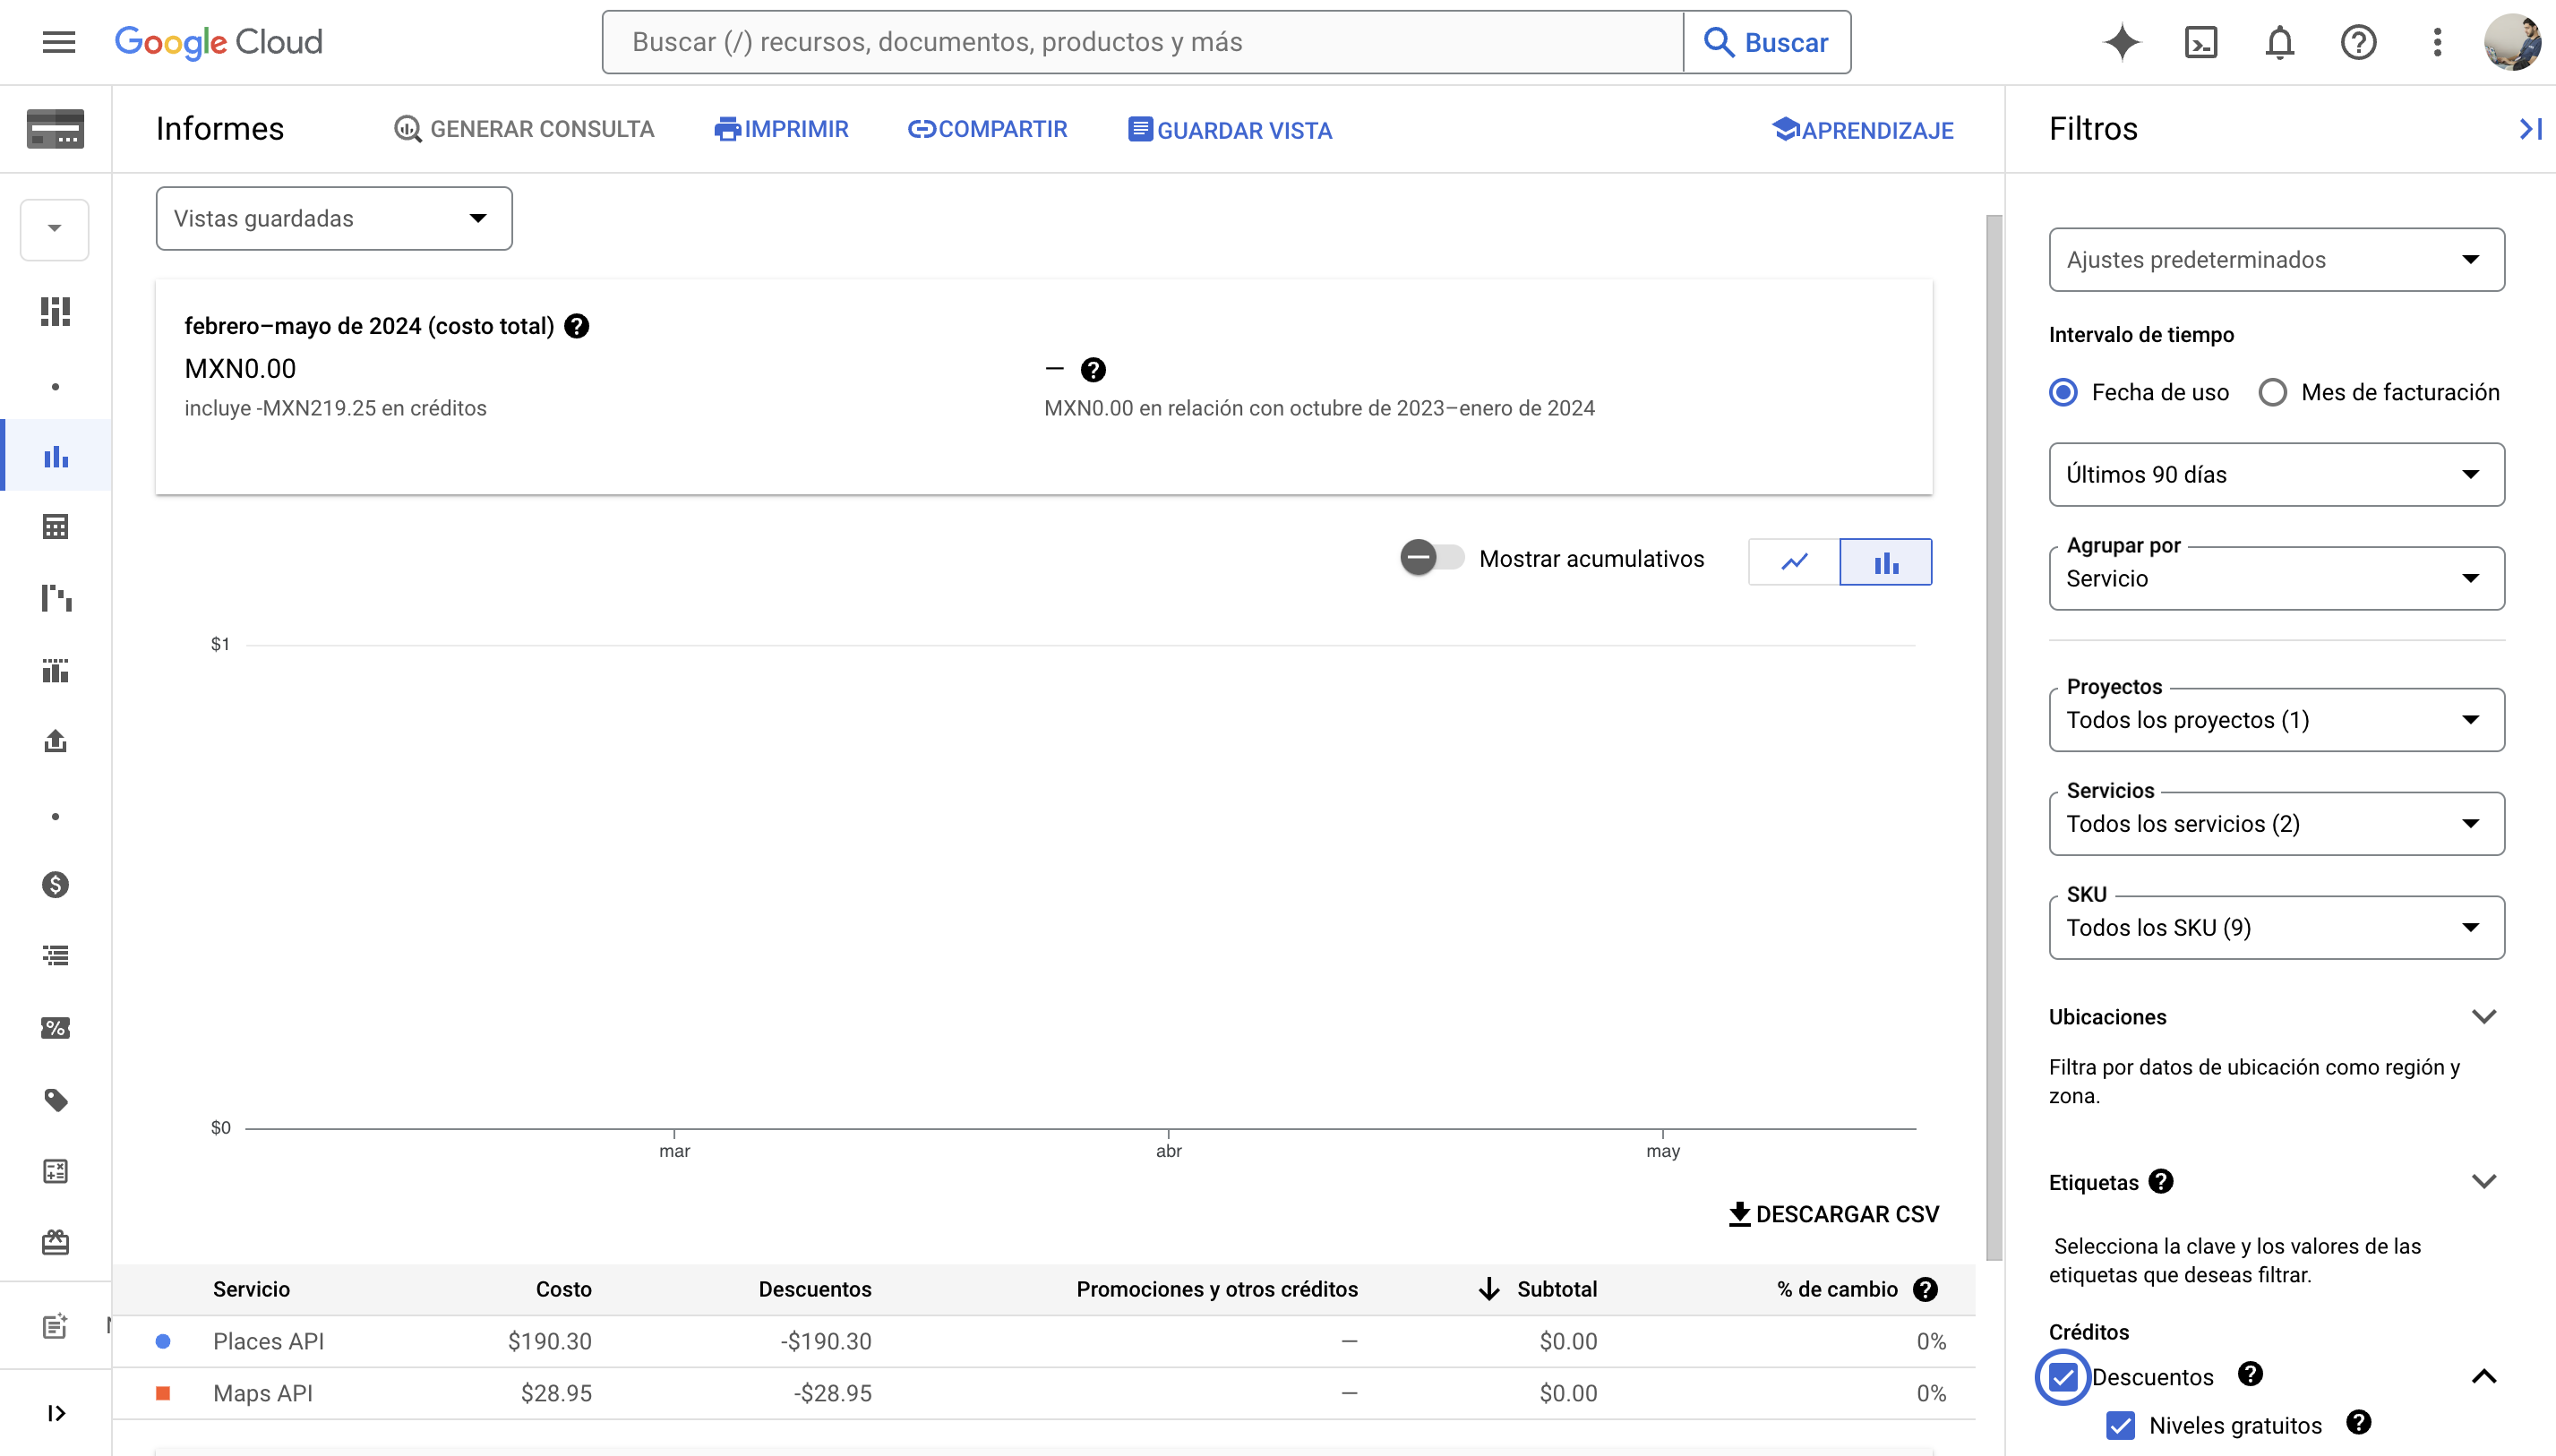
\includegraphics[width=1.0\textwidth]{imagenes/05-implementacion/costos/costos-google-maps.png}
    \caption{Costos de la API de Google Maps para la geocodificación de direcciones.}
    \label{fig:costos-google-maps}
\end{figure}

Se puede observar que el coste total de la API de Google Maps es de \$0.00 USD,
lo cual se debe al crédito inicial de \$300 USD que se ha utilizado para cubrir
los costes de las peticiones de geocodificación de direcciones.

\subsection{ExchangeRate-API}
ExchangeRate-API utiliza un modelo de precios basado en paquetes, para nuestro
proyecto se empleó el paquete gratuito que ofrece 1500 peticiones mensuales sin
coste adicional. En la figura \ref{fig:costos-exchangerate-api}
se muestra el coste registrado desde el día 23 de Abril del 2024 que es el día en
que se realizó el despliegue de la aplicación con la integración de la API de
ExchangeRate-API.

\begin{figure}[H]
    \centering
    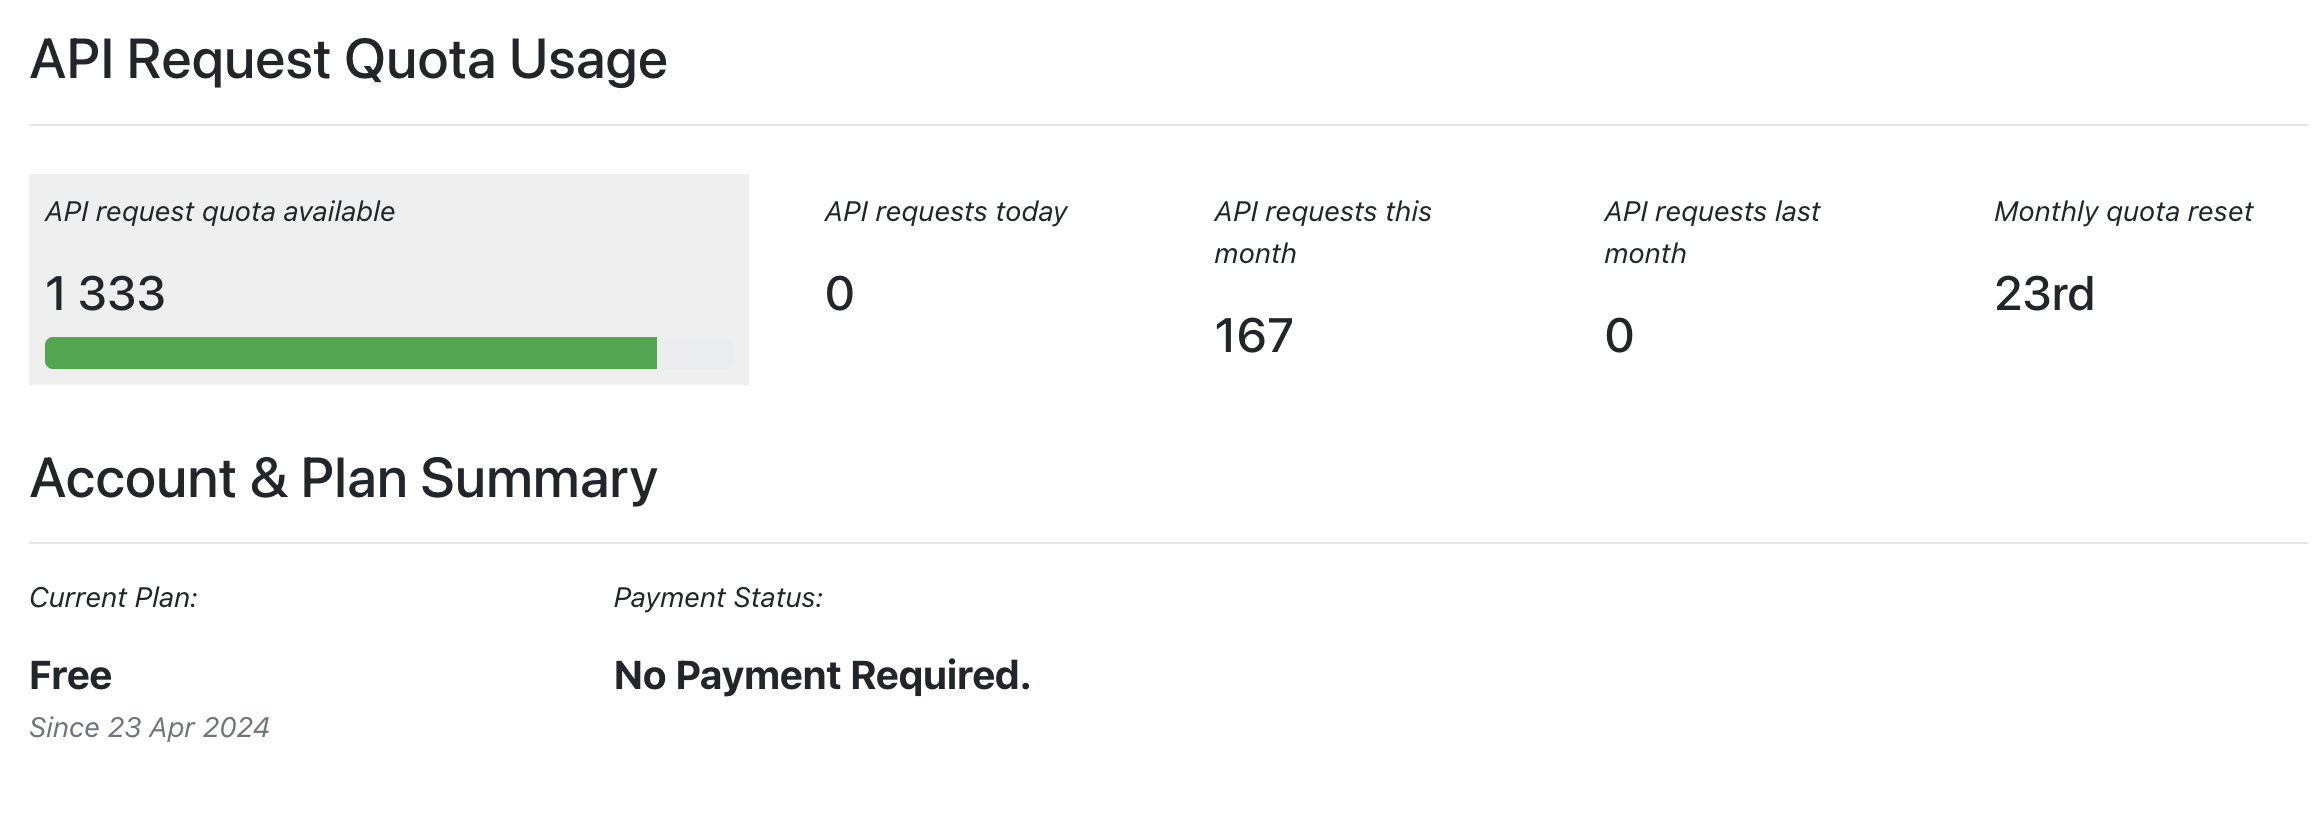
\includegraphics[width=1.0\textwidth]{imagenes/05-implementacion/costos/costos-exchangerate-api.png}
    \caption{Costos de la API de ExchangeRate-API para la conversión de monedas.}
    \label{fig:costos-exchangerate-api}
\end{figure}

Se puede osbservar que se disponen de 1333 peticiones mensuales restantes al momento
de la captura, lo cual indica que se ha utilizado un total de 167 peticiones de
conversión, lo cual nos deja con un umbral aceptable sin coste adicional.

